%---------------------------------------------------------------------------%
%-                                                                         -%
%-                           LaTeX Template                                -%
%-                                                                         -%
%---------------------------------------------------------------------------%
%- Copyright (C) Huangrui Mo <huangrui.mo@gmail.com> 
%- This is free software: you can redistribute it and/or modify it
%- under the terms of the GNU General Public License as published by
%- the Free Software Foundation, either version 3 of the License, or
%- (at your option) any later version.
%---------------------------------------------------------------------------%
%->> Document class declaration
%---------------------------------------------------------------------------%
\documentclass[twoside]{Style/ucasthesis}%
%- Multiple optional arguments:
%- [<oneside|twoside|print>]% oneside eprint, twoside eprint, or paper print
%- [fontset=<adobe|none|...>]% specify font set instead of automatic detection
%- [scheme=plain]% thesis writing of international students
%- [draftversion]% show draft version information
%- [standard options for ctex book class: draft|paper size|font size|...]%
%---------------------------------------------------------------------------%
%->> Document settings
%---------------------------------------------------------------------------%

\usepackage[super,list,table,math]{Style/artratex}
%- usage: \usepackage[option1,option2,...,optionN]{artratex}
%- Multiple optional arguments:
%- [bibtex|biber]% set bibliography processor and package
%- [<numbers|super|authoryear|alpha>]% set citation and reference style
%- <numbers>: textual: Jones [1]; parenthetical: [1]
%- <super>: textual: Jones superscript [1]; parenthetical: superscript [1]
%- <authoryear>: textual: Jones (1995); parenthetical: (Jones, 1995)
%- <alpha>: textual: not available; parenthetical: [Jon95]
%- [geometry]% reconfigure page layout via geometry package
%- [lscape]% provide landscape layout environment
%- [xhf]% disable header and footer via fancyhdr package
%- [color]% provide color support via xcolor package
%- [background]% enable page background
%- [tikz]% provide complex diagrams via tikz package
%- [table]% provide complex tables via ctable package
%- [list]% provide enhanced list environments for algorithm and coding
%- [math]% enable some extra math packages
%- [xlink]% disable link colors
\usepackage{Style/artracom}% user defined commands
%---------------------------------------------------------------------------%
%->> Document inclusion
%---------------------------------------------------------------------------%
%\includeonly{Tex/Chap_1,...,Tex/Chap_N}% selected files compilation
%---------------------------------------------------------------------------%
%->> Document content
%---------------------------------------------------------------------------%
%-
%-> Titlepage information
%-

%---------------------------------------------------------------------------%
%->> Titlepage information
%---------------------------------------------------------------------------%
%-
%-> 中文封面信息
%-
\confidential{}% 密级:涉密论文或延迟公开论文填写
\schoollogo[scale=0.095]{ucas_logo}% 校徽
\title{中国科学院大学学位论文 LaTeX 模板 }% 论文中文题目
\author{论文作者}% 论文作者
\advisor{李四~教授~中国科学院xxx研究所\\}% 指导教师:姓名 专业技术职务 工作单位
%\advisor{指导教师一\\指导教师二\\指导教师三}% 多行指导教师示例
\degree{博士}% 学位:学士、硕士、博士
\degreetype{工学}% 学位类别:理学、工学、工程、医学等
\major{计算机应用技术}% 一级/二级学科专业名称,领域名称需要与学籍信息一致
\institute{中国科学院xxx研究所}% 院系名称
%\institute{中国科学院力学研究所\\流固耦合实验室}% 多行院系名称示例
\date{2023~年~6~月}% 毕业日期:夏季为6月、冬季为12月
%-
%-> 英文封面信息
%-
\TITLE{LaTeX Thesis Template of UCAS}% 论文英文题目
\AUTHOR{Author Name}% 论文作者
\ADVISOR{Supervisor: Professor LI Si}% 指导教师
\DEGREE{Doctor}% 学位:Bachelor, Master, Doctor, Postdoctor。封面据英文学位名称自动切换,需确保拼写准确
\DEGREETYPE{Philosophy}% 学位类别:Philosophy, Natural Science, Engineering, Economics, Agriculture 等
\MAJOR{Computer Application Technology}% 二级学科专业名称
\INSTITUTE{Institute of xxx, Chinese Academy of Sciences}% 院系名称
\DATE{June, 2023}% 毕业日期:夏季为June、冬季为December
%---------------------------------------------------------------------------%
%
\begin{document}
%-
%-> Frontmatter: title page, abstract, content list, symbol list, preface
%-

\frontmatter% initialize the environment
%---------------------------------------------------------------------------%
%->> Frontmatter
%---------------------------------------------------------------------------%
%-
%-> 生成封面
%-

\maketitle% 生成中文封面
\MAKETITLE% 生成英文封面
%-
%-> 作者声明
%-
\makedeclaration% 生成声明页
%-
%-> 中文摘要
%-
\intobmk\chapter*{摘\quad 要}% 显示在书签但不显示在目录
\setcounter{page}{1}% 开始页码
\pagenumbering{Roman}% 页码符号

% 背景
% 问题
% 解决方式

混合部署是当前数据中心提升资源利用率的有效手段,通过应用对延迟的敏感度差异,可以将应用区分为延迟敏感型与尽力交付型,并部署到同一台服务器中。混合部署允许任务的并发,从而能在一定程度上提升整体资源的利用率,但由于服务器整体资源有限,并发通常会导致资源竞争,此时可以牺牲尽力交付型应用,来优先保障延迟敏感型应用的服务质量。而要实现上述目标,就依赖一定的资源隔离手段与调度机制。

本文首先对数据中心典型应用进行画像分析,分析不同应用的资源使用特征与干扰敏感度,了解应用对于运行环境的需求,以及可能存在的资源竞争场景,协助制定混部方案。其次,从内核配置与资源感知两个方面设计了针对不同场景的定制调度方案,来解决不同混部场景下的QoS保障问题。最后,为解决不同内核配置以及不同调度器在服务器上并存的需求,设计实现了Control Zone,一种面向混部场景的沙箱系统。

Control Zone基于虚拟机实现,提供了丰富的资源隔离配置,来对混部应用所需的资源进行充分的隔离与保护,同时,Control Zone支持运行时可变的调度器,通过将内核调度器容器化,能够方便地针对不同的混部方案进行选择与动态更新。而针对典型的混部场景,本文设计实现了资源感知调度策略,能根据CPU、网络等资源的使用情况来自动地进行任务调度,实现对高优先级应用的QoS保障。最后,本文还设计实现了一套围绕虚拟机的可观测性系统,能够实时地采集丰富的虚拟机指标数据,辅助进行性能分析。

% 具体数字

通过对内核以及虚拟机运行时的优化,Control Zone虚拟机启动事件能够控制在380ms以内,达到了与CloudHypervisor相近的水平。而通过响应度优先与吞吐量优先的两种内核配置,使得LC应用延迟降低了?, BE应用吞吐量提高了?。而在资源感知调度策略中,使用较为激进的调度方案,能够在保障整体CPU资源使用率的同时,使得高优先级应用的资源使用率接近其单独部署下的水平。


\keywords{数据中心,混合部署,内核调度,eBPF,服务质量}% 中文关键词
%-
%-> 英文摘要
%-
\intobmk\chapter*{Abstract}% 显示在书签但不显示在目录



\KEYWORDS{}% 英文关键词

\pagestyle{enfrontmatterstyle}%
\cleardoublepage\pagestyle{frontmatterstyle}%

%---------------------------------------------------------------------------%
% title page, abstract
\fancypagestyle{figureheader}{
  \fancyhf{}
  \fancyhead[C]{\footnotesize 图表目录}%此处填写中文标题
  \fancyfoot[C]{\footnotesize \thepage}% page number
    \renewcommand{\headrulewidth}{0.8pt}% header rule
    \renewcommand{\footrulewidth}{0pt}% footer rule
}
{% content list region
\linespread{1.2}% local line space
\intobmk*{\cleardoublepage}{\contentsname}% add link to bookmark
\tableofcontents% content catalog

\intobmk*{\cleardoublepage}{图表目录}
\thispagestyle{noheaderstyle}
{
\renewcommand*{\addvspace}[1]{}
\let\oldnumberline\numberline%
\renewcommand{\numberline}{\figurename~\oldnumberline}%
\listoffigures%
}
{
\let\cleardoublepage\relax
\let\clearpage\relax
\renewcommand*{\addvspace}[1]{}
\let\oldnumberline\numberline%
\renewcommand{\numberline}{\tablename~\oldnumberline}%
\listoftables%
}

\thispagestyle{figureheader}
}
\intobmk\chapter*{符号列表}% 显示在书签但不显示在目录

\section*{缩写}
\nomenclatureitem{AVX}{Advanced Vector Extensions}
\nomenclatureitem{BE}{Best Effort}
\nomenclatureitem{CNI}{Container Network Interface}
\nomenclatureitem{CPI}{Cycle Per Instruction}
\nomenclatureitem{CloudHP}{CloudHypervisor}
\nomenclatureitem{CZ}{Control Zone}
\nomenclatureitem{CO-RE}{Compile Once Run Everywhere}
\nomenclatureitem{eBPF}{Extended Berkeley Packet Filter}
\nomenclatureitem{FC}{Firecracker}
\nomenclatureitem{HT}{HyperThreading}
\nomenclatureitem{K8s}{Kubernetes}
\nomenclatureitem{LC}{Latency Critical}
\nomenclatureitem{LLC}{Last Level Cache}
\nomenclatureitem{NUMA}{Resource Director Technology}
\nomenclatureitem{MBA}{Memory Bandwidth Allocation}
\nomenclatureitem{QoS}{Quality of Service}
\nomenclatureitem{RDT}{Resource Director Technology}
\nomenclatureitem{SLO}{Service-level objective}
\nomenclatureitem{SIMD}{Single instruction, multiple data}
\nomenclatureitem{DSQ}{Dispatch Queue}
\nomenclatureitem{KVM}{Kernel-based Virtual Machine}
\nomenclatureitem{SIG}{Special Interest Group}
% symbol list, preface content
%-
%-> Mainmatter
%-
\mainmatter% initialize the environment
\renewcommand{\labelenumi}{(\arabic{enumi}) }
\renewcommand{\labelenumii}{(\arabic{enumi}).\arabic{enumii}}
\renewcommand{\labelenumiii}{(\arabic{enumi}).\arabic{enumii}.\arabic{enumiii}}
\renewcommand{\labelenumiv}{(\arabic{enumi}).\arabic{enumii}.\arabic{enumiii}.\arabic{enumiv}}
%---------------------------------------------------------------------------%
%->> Main content
%---------------------------------------------------------------------------%
\renewcommand{\thefigure}{\thechapter-\arabic{figure}}
\renewcommand{\thetable}{\thechapter-\arabic{table}}
\renewcommand{\theequation}{\thechapter-\arabic{equation}}
\chapter{引言}\label{chap:introduction}

\section{研究背景与意义}

% 问题 -> 
% - 数据中心规模不断扩大
% - 提升利用率的重要性
% 解决方式 -> 混部技术
% - LS 和 BE 应用天然具备混部
% - 通过混部的确解决了问题
% 局限 -> QOS
% 本质 -> 混部共享资源的竞争
% - CPU\Cache\Memory\IO\Net
% - AVX
% 研究现状
% - 劣化监测
% - 调度
% 本文

云计算提供了使用计算资源的便捷方式,其所具备弹性、安全等特征能够减轻云用户的管理负担。随着轻量级虚拟化技术的发展,LXD(Linux Container Daemon)、Docker等容器技术让应用的分发与部署更加方便,加速了应用上云的进程。同时随着容器编排技术的发展,Kubernetes、OpenShift等提供了更便捷、灵活的运维方式,催生出DevOps(Development and Operations)概念并逐渐推广。企业与普通用户越来越倾向在云平台上部署应用,不断扩张的需求催生了巨大的云计算市场。而满足庞大的市场需求,云厂商不断扩大数据中心规模,据中国信息通信研究院中国算力发展指数白皮书(2023年)显示,2022年国内数据中心机架规模超过650万个标准机架,基础算力规模达到180EFlops,位居全球第二\citep{chinaict2023}。

数据中心的庞大规模带来了巨大的治理挑战。微软Azure在其内部调研中发现,数据中心每减少1\%的资源分配碎片率,每年就能节省近1亿美元\citep{hadary2020protean}。在数据中心规模不断扩张的背景下,高效利用数据中心计算资源、提高整体资源利用率成为云厂商关注的核心问题。

将互补类型的应用部署到相同物理机上,实现数据中心资源利用率的提升是混部技术的主要方式。依据应用对延迟的敏感度,通常将应用划分为延迟敏感性(Latency Critical)与尽力交付型(Best Effort)两类。其中,LC应用通常为交互型应用,这类应用对延时十分敏感,且需要保持运行,如在线购物等。BE应用通常为离线应用,这类应用对延迟几乎没有要求,允许中断和重新运行,如大数据处理等。LC应用负载具有明显潮汐特征,向LC应用的各个空闲时段填充BE应用是混部技术提升资源利用率的核心。阿里云在实践中利用混部技术分别将集群的平均CPU利用率和内存资源利用率提升到了38.2\%和88.2\%\citep{guo2019limits}。

\begin{figure}[!htbp]
    \centering
    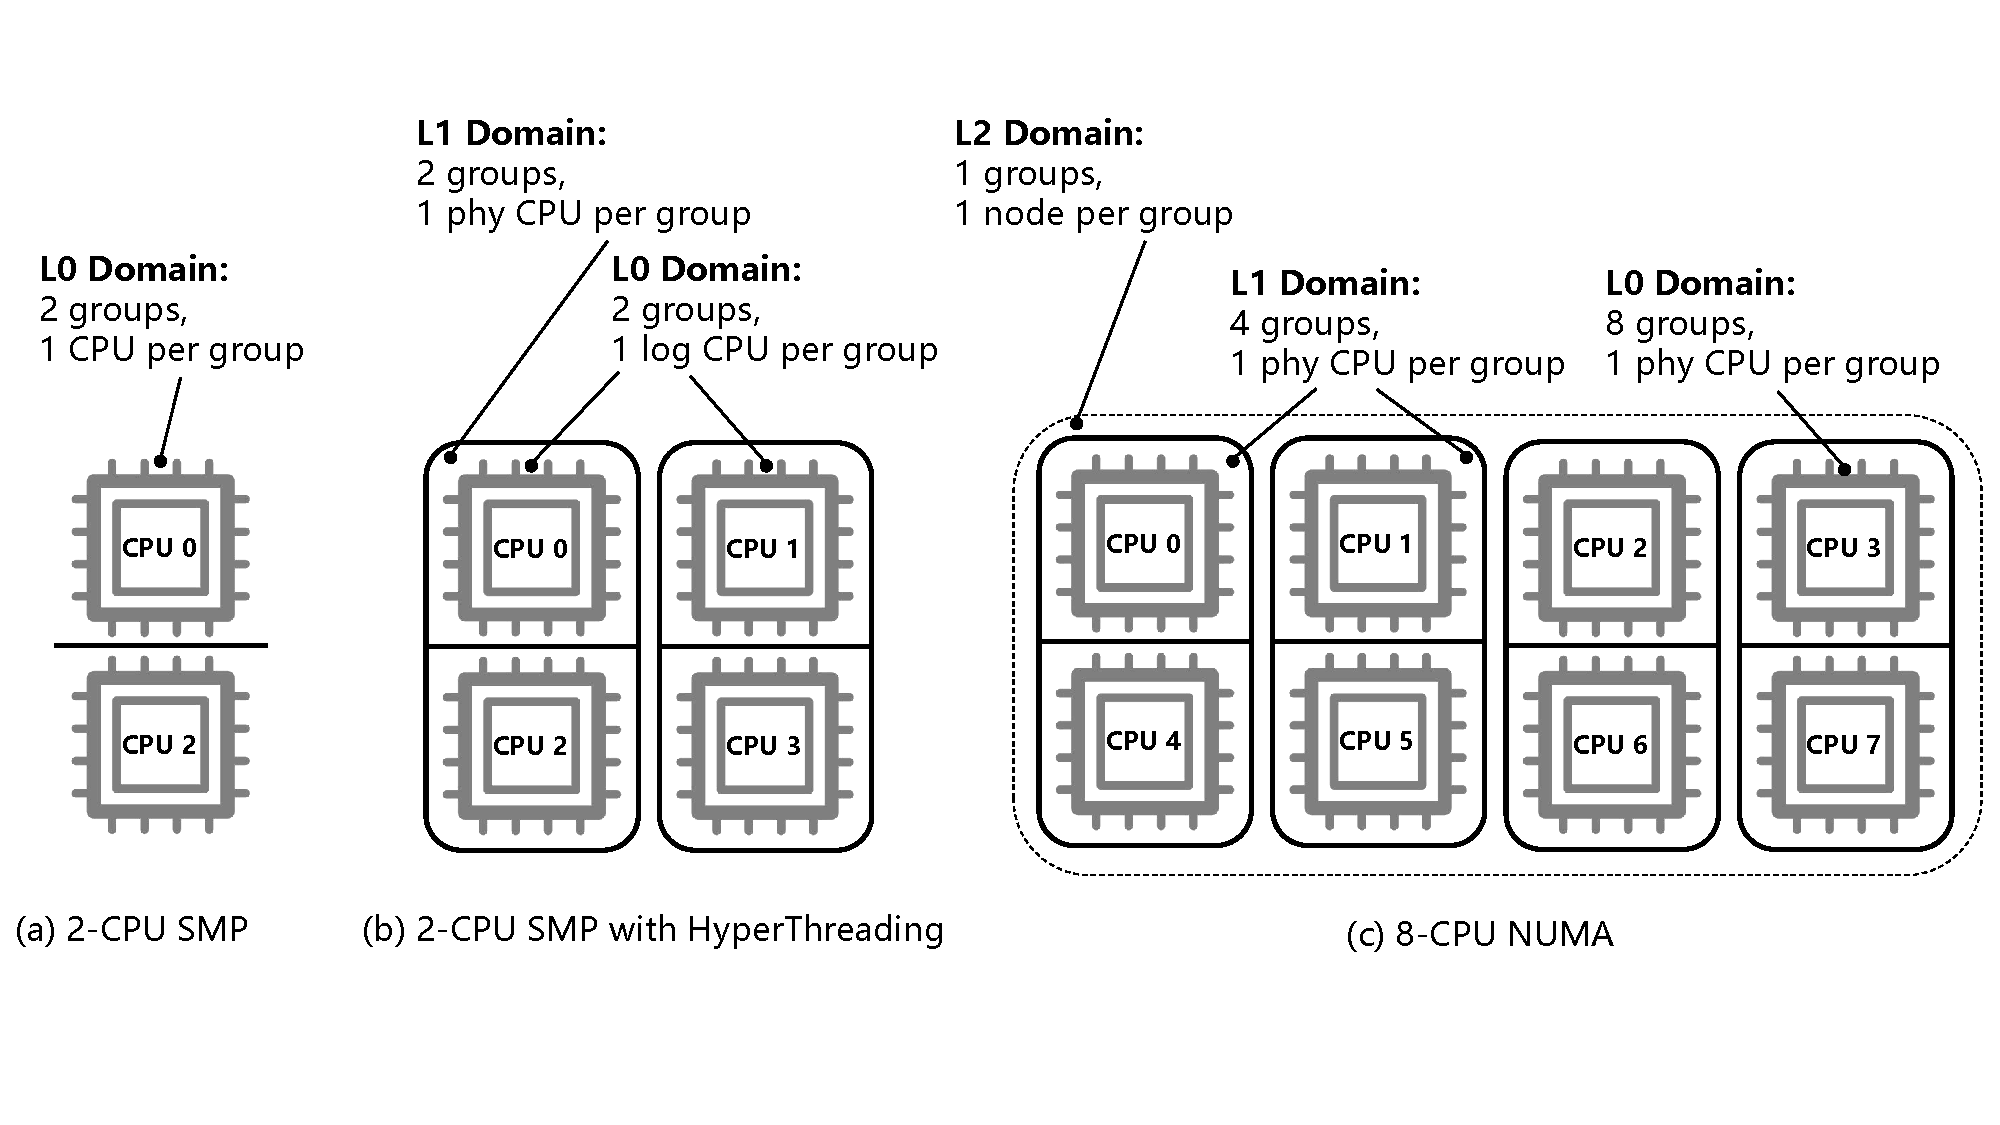
\includegraphics[width=0.85\textwidth]{scheduling_domain}
    \bicaption{\quad CPU拓扑}{\quad CPU Topology}
    \label{fig:scheduling_domain}
\end{figure}

资源竞争是混部技术下不可忽略的问题,分析这一问题首先需要了解资源的共享性与有限性。应用运行在不同的CPU上,CPU拓扑描述了核心之间的物理连接和组织方式,并反映出CPU资源的共享关系。随着CPU设计与制造技术的不断进步,当前出现如超线程技术(Hyper-threading)、非同一内存访问架构(NUMA)、大小核心架构等新特性,CPU拓扑也越来越复杂。常见的CPU拓扑如图~\ref{fig:scheduling_domain}所示,逻辑核位于CPU拓扑的最低一层,任务分时复用逻辑核资源,某一时刻仅有一个任务在运行,彼此几乎没有影响。超线程技术最早于2002年由Intel提出,通过增加部分片上资源使得一个物理核上能够运行多个逻辑核。超线程技术下的片上资源分布如图~\ref{fig:cpu_topology}所示,兄弟核心拥有各自独立的寄存器组与中断控制器,但彼此共享了执行单元、Cache和总线等其他资源。NUMA(非一致存储器访问)架构中存在多个CPU模块,每个CPU模块可包含多个CPU,这些CPU拥有自己的本地内存与IO接口,但彼此共享了相同的内存总线与LLC,且在IO资源上相互竞争。

\begin{figure}[!htbp]
    \centering
    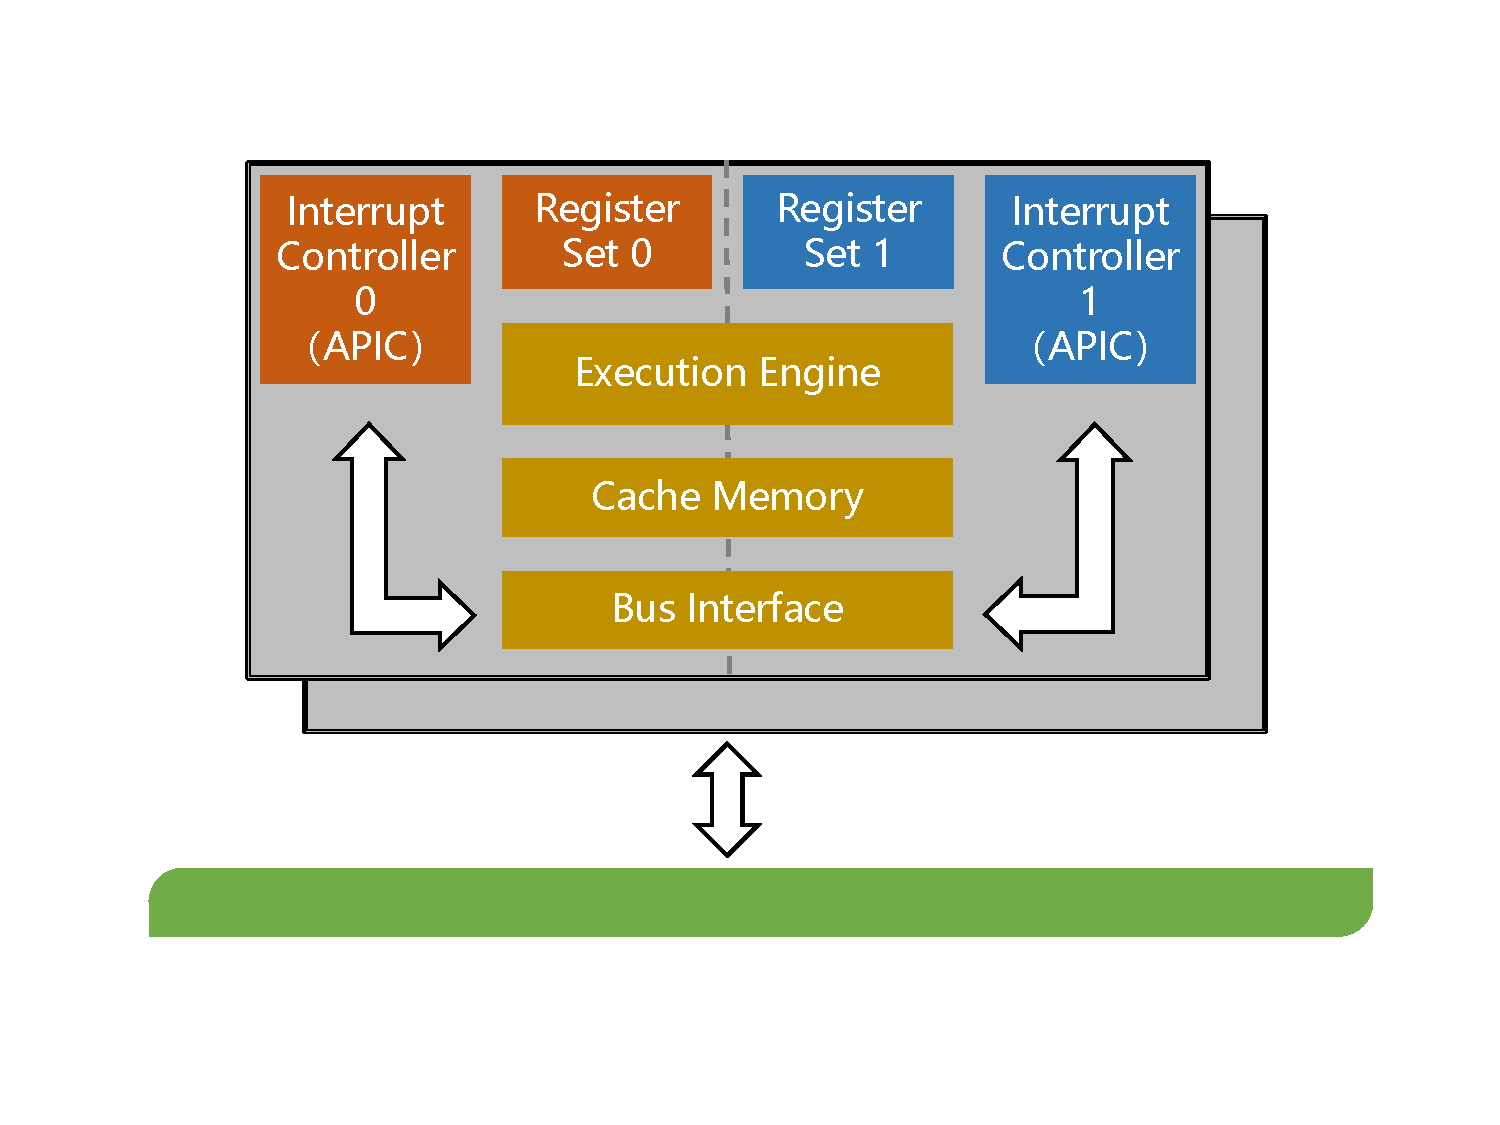
\includegraphics[width=0.5\textwidth]{cpu_topology}
    \bicaption{\quad Siblings片上共享资源 }{\quad Siblings on-chip shared resources}
    \label{fig:cpu_topology}
\end{figure}

现代服务器计算资源丰富,支持大量应用同时运行,然而服务器局部硬件资源有限,如片上资源、LLC、内存带宽、网络带宽等都存在明确的限制。混部技术向单一物理机上部署了更多的任务,增大了局部硬件资源竞争的概率,并容易造成应用QoS的劣化。如在网络子系统中,没有竞争到足够网络带宽的任务会在队列中积压,并导致应用延迟的激增。数据中心应用数量多、软件环境复杂,不同应用对资源的需求各不相同,一方面应用间存在隐含的资源竞争,另一方面应用竞争不同资源所引发的QoS劣化程度也存在差异。

资源竞争引发的QoS劣化体现在应用的性能指标上。云厂商提供了SLO来允许用户定义云应用的期望状态。SLO包含服务可用性、带宽等基础指标,以及每秒请求数量、尾延迟等业务性能指标。云厂商通过与用户协商SLO来提供云产品QoS的保证,并在违反SLO时进行补偿。应用的QoS劣化不仅会为云厂商带来经济损失,还会引发用户的流失,因此保障应用QoS是混部场景下云厂商核心需求。混部场景下QoS保障相关研究通常从三个方向展开:

\begin{enumerate}

    \item 利用可观测性技术监测应用的QoS,并收集数据进行画像分析。云厂商依赖可观测性基础设施来对数据中心进行持续监测。可观测性基础设施围绕不同的软件环境设计,如面向虚拟机、面向容器编排系统等。通过全面地指标监测实时收集数据,不仅可以及时发现应用的QoS劣化并进行预警,还能够利用丰富的指标数据来进行细致的画像分析,挖掘更多的混部机会。Google在2011年公布了混部集群监控数据集,阿里云也在2017年公开了一部分混部集群的监控数据集\citep{guo2019limits},这些来自生产环境的脱敏数据集,大大促进了基于数据分析的QoS劣化监测研究。

    \item 围绕资源隔离的混部场景QoS保障研究。资源隔离即通过软硬件手段来强化混部场景下应用在共享资源上的隔离性,防止因敏感资源竞争导致的应用QoS劣化。不同资源隔离技术的区别在隔离资源的类型与粒度上,如使用Cgroup技术对CPU资源隔离,或使用Traffic Control技术\citep{hubert2002linux}对网络带宽隔离。同时,基于硬件级资源隔离技术能实现更细粒度的隔离效果,如隔离末级缓存与内存带宽。组合这些隔离技术来制定不同的调度策略是基于资源隔离混部研究的主要方式。

    \item 围绕任务调度的混部场景QoS保障研究。任务在被调度到CPU上时才能执行,并进一步申请其他的硬件资源,因此CPU资源是大部分硬件资源分配的起点。相关研究从任务调度延时与灵活性上展开。其中微秒级调度机制通过远低于应用延迟要求的调度延时,及时分配CPU资源来避免QoS劣化。灵活的任务调度机制通过修改任务调度的逻辑,针对混部场景应用与硬件特性进行适量身定制,从而更好地进行QoS保障。

\end{enumerate}

% 而了解应用的状态变化,实施精准的调度是解决混部场景中QoS保障问题的核心

\section{国内外相关研究}

\subsection{数据中心可观测性与劣化监测研究现状}

% 可观测性技术
% - 定义
% - 实践

可观测性技术指通过指标监控、日志记录、链路追踪和其他数据收集手段来描述系统的状态,协助理解和诊断系统的行为和性能。在指标监控上,开源社区Prometheus\citep{brazil2018prometheus}定义了一种时序数据结构Metric,以及围绕Metric的高效的编解码机制、灵活的数据存储方式和便捷的PromQL查询语言。此外,Prometheus社区还提供了采集系统的标准实现,包含Promethues Server、Node Exporter等核心组件,并与Grafana社区协作推出开源的数据展示服务。Promethues完全开源且致力于完善多语言库支持。在各云厂商及开源社区开发者的共同参与下,Prometheus社区发展迅速,并逐渐成为指标采集领域的现行标准。

随着软件架构的迭代,可观测性技术也在不断进步。微服务是数据中心常见的软件架构,其中一次请求调用链路往往跨越多个进程与服务器。传统的进程观测手段难以有效地对微服务进行观测,而为解决这一问题,Google在2010年提出了分布式链路追踪系统Dapper\citep{sigelman2010dapper},用于对微服务应用进行性能分析。Dapper的设计如图~\ref{fig:dapper_trace}所示,其中Trace用来记录一次完整的链路追踪,Span用来记录链路中的单个操作。单个操作可以是一次函数的调用或者一段代码块,Dapper需要在代码插桩以指示Span的生成。在函数调用的过程中,Span会作为上下文的一部分传递,并自动地构建调用关系。而微服务中一次函数调用也可以是一次远程过程调用(RPC),此时Dapper会将Span注入到网络报文的载荷中,让Span跨进程、服务器地传递下去。Span最终发送到Dapper的分析系统,并根据树形关系重建得到完整的Trace,实现一次链路追踪过程。OpenTracing和OpenTelemetry等开源项目吸收了Dapper的核心思想,并在云原生社区中迅速推广。链路追踪依赖代码插桩,对编译型语言来说需要修改源代码,因此接入十分不便。而在容器编排系统中则通过Overlay Network来实现无侵入的微服务性能观测。Kubernetes中提供了CNI(Container Network Interface)\citep{k8s-network-plugins},允许开发者自定义容器网络模型。开源CNI项目Cilium\citep{cilium}基于eBPF、Envoy等技术\citep{ebpf,envoyproxy}实现集群的Overlay Network,提供从L3、L4到L7的网络观测能力,并无需侵入用户代码。

\begin{figure}[H]
    \centering
    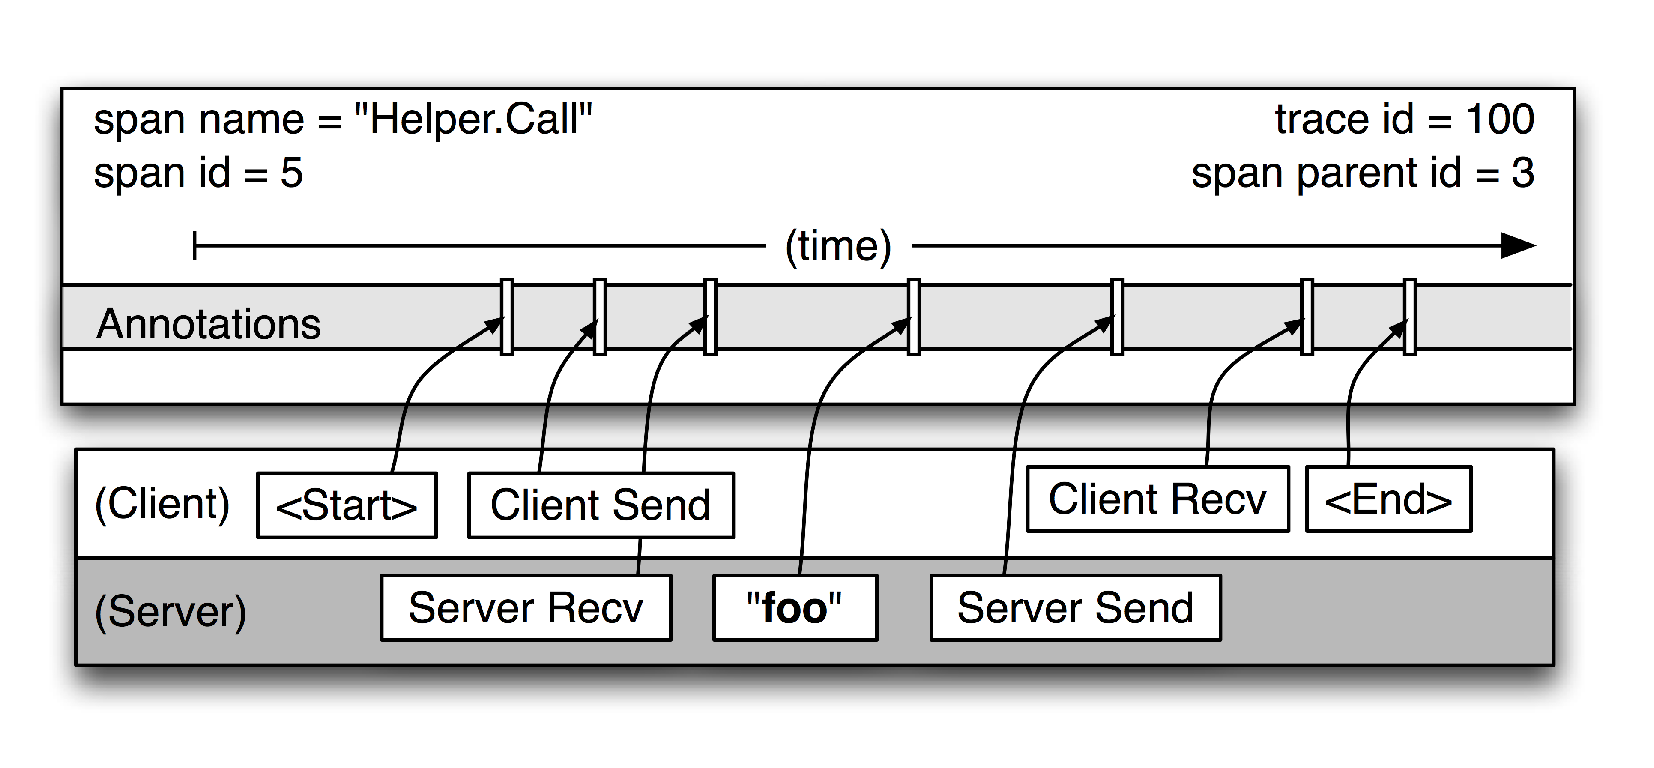
\includegraphics[width=0.6\textwidth]{dapper_span}
    \bicaption{\quad Dapper链路追踪流程(图片引用自文献\citep{sigelman2010dapper})}{\quad Dapper tracking process (picture quoted from paper\citep{sigelman2010dapper})}
    \label{fig:dapper_trace}
\end{figure}

近年来随DevOps技术的发展,可观测性技术在云服务中占据了越来越重要的地位。而基于采集得到的指标分析应用性能劣化情况是可观测性技术的主要应用场景。云厂商在早期实践中倾向一些简单的指标。如Google就使用CPI(Cycle Per Instruction)\citep{zhang2013cpi2}来反映应用的性能。CPI本身用于度量微观体系结构下的性能。应用正常运行时CPI通常会在一个小范围内波动。而当应用性能劣化时,CPI波动范围则会显著变化。CPI作为一个简单指标在许多场景都有效,但在CPU频率较低时会出现一定误差。Li Yi等人\citep{yi2020cpi}观察到这一现象,在CPI基础上优化得到RCPI,并修正了误差。

数据中心的监控数据数量多、维度广,支持多样的手段来进行数据分析。近年来随AI技术的发展, 结合AI技术和数据中心QoS劣化监测的研究不断展开。相关研究的核心在于如建立AI模型来预测应用的QoS劣化,从而实现提交发现和预先调度\citep{qiu2020firm, zhou2022aquatope, wang2022deepscaling, gan2021sage, ghafouri2020survey,zheng2020web,wu2019posterior}。其中
FIRM\citep{qiu2020firm}面向Kubernetes集群设计了一种两级的机器学习模型,能精准预测集群中应用的QoS劣化。Di Wu\citep{wu2020data}则提出了一种数据特性感知潜在因素(DCALF)模型来实现高精度的QoS预测,同时能针对不同数据的特点区别地处理。以上研究在调度延时不敏感、应用变化相对慢的集群取得了相当显著的QoS劣化监测与调度效果。

\subsection{围绕资源隔离的混部场景QoS保障研究现状}

% 集群维度: 放置策略
% 单点维度: 细粒度分配

数据中心的资源通常可划分为集群资源与节点资源。其中,集群资源天然通过不同的机器、机架隔离开,相关研究侧重于解决应用的放置问题。集群中各节点都部署了可观测性基础设施,能汇总各节点的资源使用情况。当应用需要调度时,集群调度器通过评估各节点的资源使用情况和应用的资源需求,来选择合适的节点进行部署。集群调度器算法能否给应用分配足够的资源是影响应用QoS的关键。Protean\citep{hadary2020protean}是微软Azure的集群调度器,主要负责用户虚拟机的调度。Protean的决策过程包括地域、地区、机柜三个层次。每一层都设置独立的算法,依据当前层的资源分配情况进行决策,并逐层求解出最优位置。Protean最终选定的位置能够确保为虚拟机提供足够的资源,从而保障虚拟机的QoS。

节点资源有一定的隔离性,同时存在丰富的软硬件手段来进一步强化隔离性。软件上,Linux各资源子系统提供了丰富的资源隔离机制,包括Cgroup、Traffic Control等。硬件上,芯片制造厂商通过在硬件上引入额外特性,实现更细粒度的隔离机制。如针对内存带宽、末级缓存等资源,各大CPU厂商均提供了相关的硬件调控技术,包括Intel Resource Director Technology(Intel RDT)\citep{guide2011intel}、AMD Platform Quality of Service Extensions(AMD PQoS)\citep{amdpqos}、ARM Memory System Resource Partitioning and Monitoring(ARM MPAM)\citep{armmpam}等。节点上更细粒度的资源隔离手段能够有效协助解决"吵闹邻居"问题\citep{xu2018dcat, maricq2018taming, rzadca2020autopilot, kwon2020dc}。

\begin{figure}[!htbp]
    \centering
    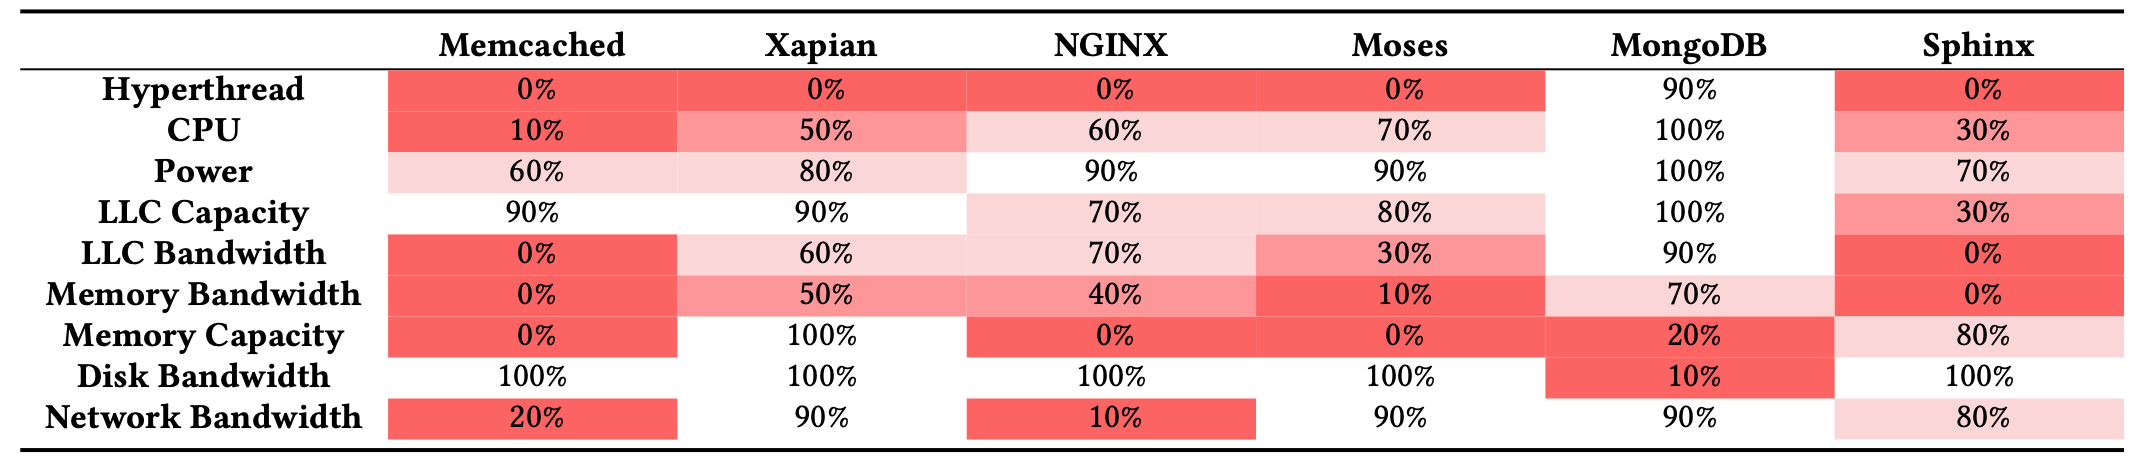
\includegraphics[width=0.85\textwidth]{parties_app_dif}
    \bicaption{\quad 不同资源干扰对应用性能的影响(图片引用自文献\citep{chen2019parties})}{\quad diferent resource interference on application performance(quoted from paper\citep{chen2019parties})}
    \label{fig:parties_app_dif}
\end{figure}

基于节点资源的隔离性,部分研究围绕放置策略展开。Paragon\citep{delimitrou2013paragon}将推荐系统中常用的协同过滤技术(Collaborative filtering technique)引入到放置问题中,通过预测应用对节点上其他应用的影响以及应用能够承受的干扰,来进行应用的放置决策,实现了大多数工作负载场景下的QoS保障。而结合丰富的节点资源隔离手段,部分研究通过避免应用在关键资源上的竞争来实现应用的QoS保障。Quasar\citep{delimitrou2014quasar}预先对应用进行画像分析,并建立分类模型。随后通过分类模型快速确定新应用的资源需求以及干扰的敏感度,并利用资源隔离技术来调整资源分配。Heracles\citep{lo2015heracles}从应用资源敏感度的角度入手,分析了不同应用在不同负载下对于多种资源的敏感度,并依据分析结果优先保证敏感资源供给,从而实现应用的QoS保障。Parties\citep{chen2019parties}则进一步分析了如图~\ref{fig:parties_app_dif}所示更丰富的资源种类。在调度上,不同于Heracles,Parties利用应用间的资源拆借,实现保障应用QoS的同时整体资源利用率也得到提升。CLITE\citep{patel2020clite}利用贝叶斯优化构建资源隔离模型,将多个LC应用与BE应用进行混部,并利用Intel MBA技术对内存带宽进行控制以保障LC应用的QoS。LIBRA\citep{zhang2021libra}则基于一种新型硬件节流机制,实现内存带宽的动态调控,并根据应用的需求变化动态调整,及时地保障内存带宽资源供给。

\subsection{围绕任务调度的混部场景QoS保障研究现状}

% 内核任务调度
% 微秒级调度

围绕任务调度的QoS保障研究聚焦于CPU资源的分配,相关研究围绕调度机制的设计展开。调度机制的核心在于调度延时与调度策略,其中调度延时通常与Runtime的实现相关,而调度策略则取决于不同混部场景的调度目标。

CFS调度器\citep{pabla2009completely}于2009年提出,用来解决交互式应用与非交互式应用在调度上的公平性问题。CFS的核心在于CPU vruntime的计算与维护。CFS调度器为Run Queue中的每一个调度实体维护一个时间记账,并在每个时钟中断处理中更新。而在每个调度循环中,CFS会调度Run Queue中vruntime最小的任务执行。CFS调度器长期以来都是Linux的默认调度器,但存在灵活性的不足,难以满足当前数据中心应用的需求。为解决CFS的灵活性问题,Linux 6.6版本中引入了EEVDF(Earliest Eligible Virtual Deadline First)调度器。EEVDF调度器\citep{stoica1995earliest}于1995年提出,其中调度器会为每个进程维护一个虚拟截止时间,并在每次调度时选择最早截止时间的任务执行。不同于CFS,EEVDF调度器的优先级设计考虑到了应用对时间片的不同需求,并增加了latency-nice机制。如图~\ref{fig:eevdf_scheduling}所示,为任务设置较高的latency-nice值会让任务总是获得长而少的时间片,这样能够减少上下文切换的次数,对于计算密集型的应用而言有利于提高吞吐。而为任务设置较低latency-nice值则会让任务总是获得短而多的时间片,这样能够让CPU资源更快地分配,从而提升应用的响应度。

\begin{figure}[!htbp]
    \centering
    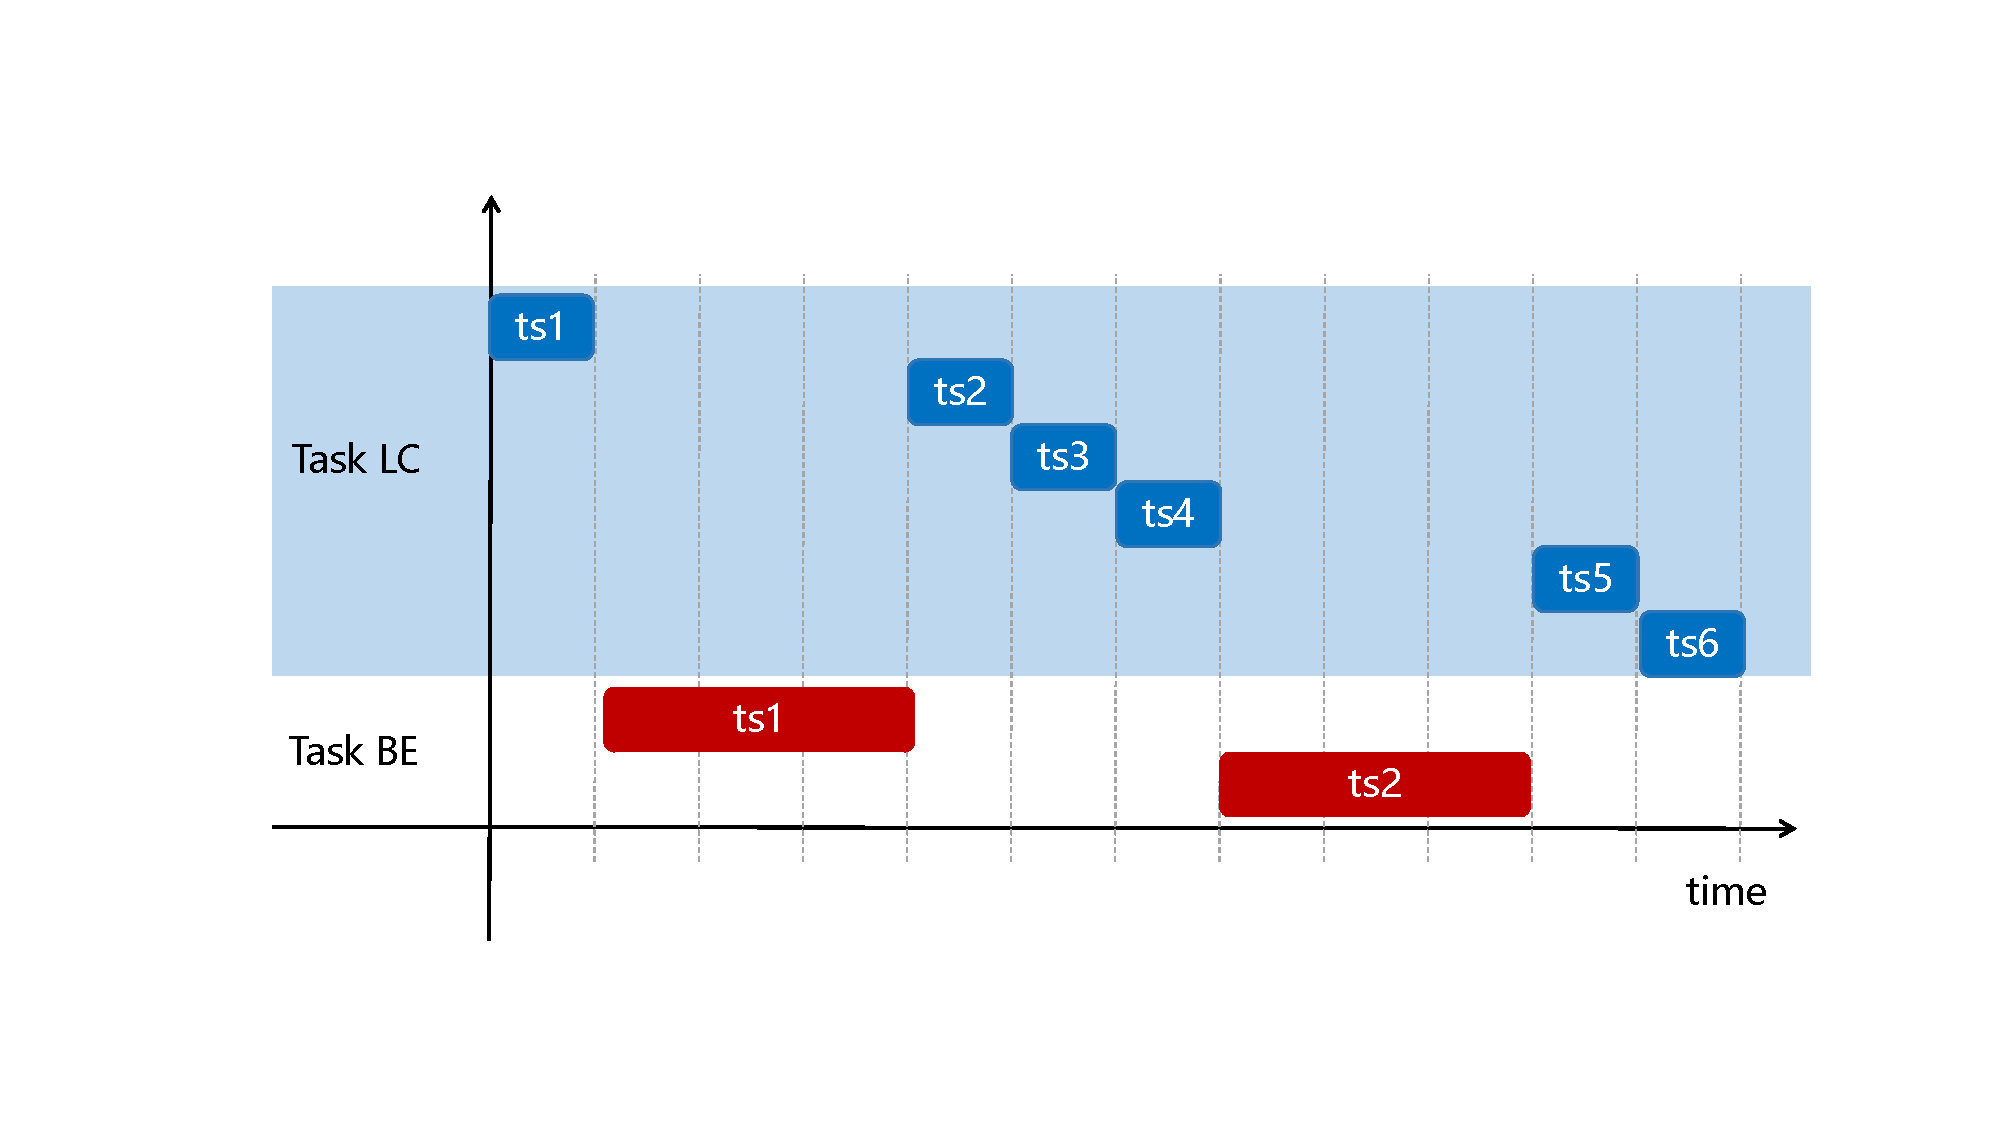
\includegraphics[width=0.65\textwidth]{eevdf_scheduling}
    \bicaption{\quad EEVDF可变时间片机制}{\quad EEVDF Variable Time Slice Mechanism}
    \label{fig:eevdf_scheduling}
\end{figure}

针对CPU拓扑,Linux 2.6中引入了调度域(Scheduler Domains)\citep{schedulerdomains},用来协助处理多核处理器上的调度。如表~\ref{tab:resourcesharing}所示,不同调度域充分反映了对于CPU拓扑上的资源共享信息。而调度子系统可基于调度域这层抽象来了解CPU间的差异性,进而针对性地进行调度。然而Linux任务调度机制在处理不同调度域时仍有不足:

\begin{itemize}
    \item 超线程调度域中兄弟核心存在如表~\ref{tab:resourcesharing}所示的共享资源,部署在兄弟核心上的应用存在竞争的可能。Elfen\citep{yang2016elfen}设计了一种新的内核调度机制,首先提供了一种全新的系统调用nanonap,允许进程快速地释放CPU资源但保留对CPU的所占有状态。同时,Elfen通过向BE应用插入探测代码,使得BE应用在运行过程中能够快速的探测兄弟核心上任务的运行并及时调用nanonap释放资源。通过以上设计,Elfen实现了LC应用与BE应用在部署到兄弟核心时的交替执行,从而避免因资源竞争导致的QoS劣化。 

    \begin{table}[!htbp]
        \bicaption{\quad 调度域与共享资源}{\quad scheduler domains and resource sharing}% caption
        \label{tab:resourcesharing}
        \footnotesize% fontsize
        \setlength{\tabcolsep}{4pt}% column separation
        \renewcommand{\arraystretch}{1.5}% row space 
        \centering
        \begin{tabular}{lc}
            \hline
            %\multicolumn{num_of_cols_to_merge}{alignment}{contents} \\
            %\cline{i-j}% partial hline from column i to column j
            调度域 & 共享资源\\
            \hline
            Core & 几乎隔离\\
            SMT & 执行单元、缓存、总线\\
            NUMA & 末级缓存、内存带宽、IO\\
            \hline
        \end{tabular}
    \end{table}

    \item 部分片上资源存在隐含的竞争破坏了调度域的隔离性。AVX(Advanced Vector Extensions)指令属于SIMD的一部分,旨在提高CPU的浮点运算性能,最早由Intel提出并于2011开始在实际产品中加入。AVX指令涉及到CPU中加速单元的使用,而使用加速单元意味着更高的能耗。为防止过热,现代CPU通常会在加速单元工作时降低运行频率。这就引发了两个Linux任务调度上的公平性问题\citep{gottschlag2020avx}。首先,由于CPU频率的恢复需要一定的时间,当同一Core调度域中的任务切换发生在恢复过程中时,就存在相互影响的可能。其次,兄弟核心共享了同一个物理核,物理核心的频率会使得所有兄弟核心受到影响。为解决这两个公平性问题,Gottschlag\citep{gottschlag2021fair}对现有调度机制进行了修改。首先,Gottschlag设计了一种监测手段,能够通过向量寄存器的使用情况来判断是否有AVX指令的执行。随后,Gottschlag在任务调度机制中增加了vruntime补偿逻辑,通过调整受影响的Core调度域与SMT调度域上的任务的vruntime来解决公平性问题。
\end{itemize}

另一种通过任务调度保障混部应用QoS的思路是微秒级调度\citep{ousterhout2019shenango,fried2020caladan,prekas2017zygos},其核心在于将调度延时降低到LC应用允许的延迟范围内,及时分配CPU资源来避免应用QoS劣化。Caladan\citep{fried2020caladan}实现了一种用户态的任务运行时,并通过DPDK(Data Plane Development Kit)、SPDK(Storage Performance Development Kit)解决硬件驱动问题。Caladan将操作系统的大部分功能实现到用户态,一方面去除了地址空间隔离,能够大大减少上下文切换的开销。另一方面打破Linux调度子系统的限制,能够更灵活地开发调度策略。Caladan使用集中式的调度模式,在负责调度的核心上基于高精度时钟实现微秒级调度延时。同时,Caladan能够从DPDK、SPDK中读取硬件资源的分配状况,这些额外信息能够有效辅助进行调度决策。

为特定工作负载量身定制调度策略能够显著改善如延时、吞吐量、能效等关键指标,然而在大型数据中心设计、实施和部署新的任务调度策略是一项艰巨的任务\citep{humphries2021ghost}。首先,调度子系统涉及Linux内核中的许多复杂机制,如复杂的同步原语及P-state(Processor State)控制等,独立开发的难度较大。其次,Linux内核开发不同于普通用户程序,可用程序库较少,且对代码编写有严格的限制与规范。部署新调度策略时,由于Linux无法在运行时重载调度子系统,因此通常需要重新启动。而服务器的重启意味着反复的任务迁移,这在生产环境是难以接受的。最后,Linux社区在调度子系统的迭代上相对保守,并期望实现普适的调度策略,一个高质量的调度器通常需要数十年的时间来不断完善\citep{agache2020firecracker},如EEVDF调度器从提出到正式并入主线内核就花费了29年。

为解决内核调度器在设计、实施和部署上的问题,加速内核调度机制迭代,Google提出了ghOSt\citep{humphries2021ghost}用户态调度器框架。ghOSt框架中包含三部分:内核调度类、用户态调度器及调度信息协议。其中,内核调度类在内核侧不断地更新任务状态,并按协议生成调度事件。用户态调度器通过特殊的系统调用消费事件并进行调度决策。而决策同样以事件的形式通过特殊系统调用提交到内核调度类,并进行真正地实施。ghOSt调度框架在一定程度上解决了内核调度的灵活性问题,但由于频繁系统调用所引发的上下文切换开销,难以实现较低的调度延时。eBPF技术提供了一种对Linux现有功能动态修改的思路,但仅在网络子系统中有较成熟的实践。Meta与内核社区的开发者共同创建了Sched Ext项目,提供了一种使用eBPF技术定制Linux调度机制的方式。相较于ghOSt,Sched Ext完全运行在内核中,能够实现更低的调度延时。同时,Sched Ext能够借助eBPF在其他子系统中的探测能力获取丰富的信息来辅助调度决策,实现更好地应用QoS保障。

\section{论文的研究内容}

本文主要研究单点混部场景QoS保障问题,综合以上相关理论研究能够发现:

\begin{enumerate}

    \item \textbf{数据中心传统应用划分形式单一,容易忽略应用在资源上的倾向性与敏感性}。这一方面容易引发混部应用在隐含资源上竞争,另一方面也不利于系统资源的充分利用。在观测指标上,相关研究表明单一指标在部分场景中有效,但同时也依赖多维度、广泛的数据采集来对应用进行充分性能分析。最后,AI技术在集群调度上能够很好的发挥作用,但对于节点侧尤其是内核调度上,AI技术存在实施与部署上困难的问题。
    
    \item \textbf{任务调度机制是解决单点混部场景QoS保障问题的核心}。数据中心LC应用大部分为服务型应用,其资源使用倾向与敏感度随负载变化而变化。负载的动态性要求调度机制能够迅速的做出反应。基于资源隔离的调度程序一般在用户态实现,依赖系统调用来获取资源分配信息和进行资源隔离。同时,资源隔离机制存在一定的生效延迟。这都限制了调度程序的调度频率,不利于应用的QoS保障。不同于资源隔离,任务调度则通过CPU资源分配来间接地控制应用的资源使用。尽管调控粒度较粗,但由于在调度速度上的优势,任务调度能够更好地在单点上保障混部应用的QoS。
    
    \item \textbf{应用动态特性要求更灵活的任务调度机制,且单一的任务调度机制无法在各个混部场景有效}。Linux内核追求普适的调度机制,并存在大量的启发式逻辑,难以针对特定混部场景进行调整与定制。其次,Linux调度机制在编译时确定且无法在运行时修改,在软硬件环境发生变化时不能快速调整。微秒级任务调度机制虽然QoS保障效果优秀,但由于绕过内核的设计与高度的定制,存在兼容性问题,无法在生产环境中大规模使用。最后,服务器资源丰富,能够同时运行大量应用,这些应用构成多样的混部场景。而相关研究通常针对特定的混部场景,无法保证在各个混部场景下有效。

\end{enumerate}

综合上述对混部场景QoS保障研究的分析,本文总结了如下挑战并开展相应工作:

\begin{enumerate}

    \item \textbf{针对数据中心的软件环境复杂性挑战,展开典型应用监测与画像分析研究}。首先,结合对数据中心软件栈分析以及与云厂商的合作经验,选择了一批典型应用作为画像目标,并采用虚拟机作为应用的运行环境。随后,设计实现了黑匣子(Black Box)观测系统,围绕虚拟机在Host、Hypervisor与App等多重维度,采集丰富的指标信息。最后,在Black Box观测系统的基础之上,展开针对典型应用的资源倾向与敏感度实验并给出画像结论。

    \item \textbf{针对当前任务调度机制在不同混部场景下的不足,展开混部场景导向的定制任务调度机制研究}。首先,从内核任务调度的相关配置上针对不同应用的需求,设计了响应度优先与吞吐量优先两种基础内核配置。随后,在Ext调度类的基础上设计了塔台(Control Tower)任务调度框架,并在此基础上,结合eBPF技术的监测能力进一步实现CPU资源感知与网络资源感知的任务调度策略。

    \item \textbf{针对单一调度机制与多样混部场景的挑战,设计实现受控空域(Control Zone),一种面向混部场景的调度动态可定制沙箱}。Control Zone基于KVM虚拟机实现,如图~\ref{fig:arch_dif}所示,相较于Firecracker\citep{agache2020firecracker},Control Zone允许将Control Tower调度策略与混部应用协同部署。一方面,能够针对不同混部场景自由地选择合适的Control Tower调度策略。另一方面,能够随混部应用的变化在运行时对Control Tower调度器动态修改。同时,还支持通过软硬件手段来隔离不同Control Zone的资源。

\end{enumerate}

\begin{figure}[!htbp]
    \centering
    \begin{subfigure}[b]{0.4\textwidth}
        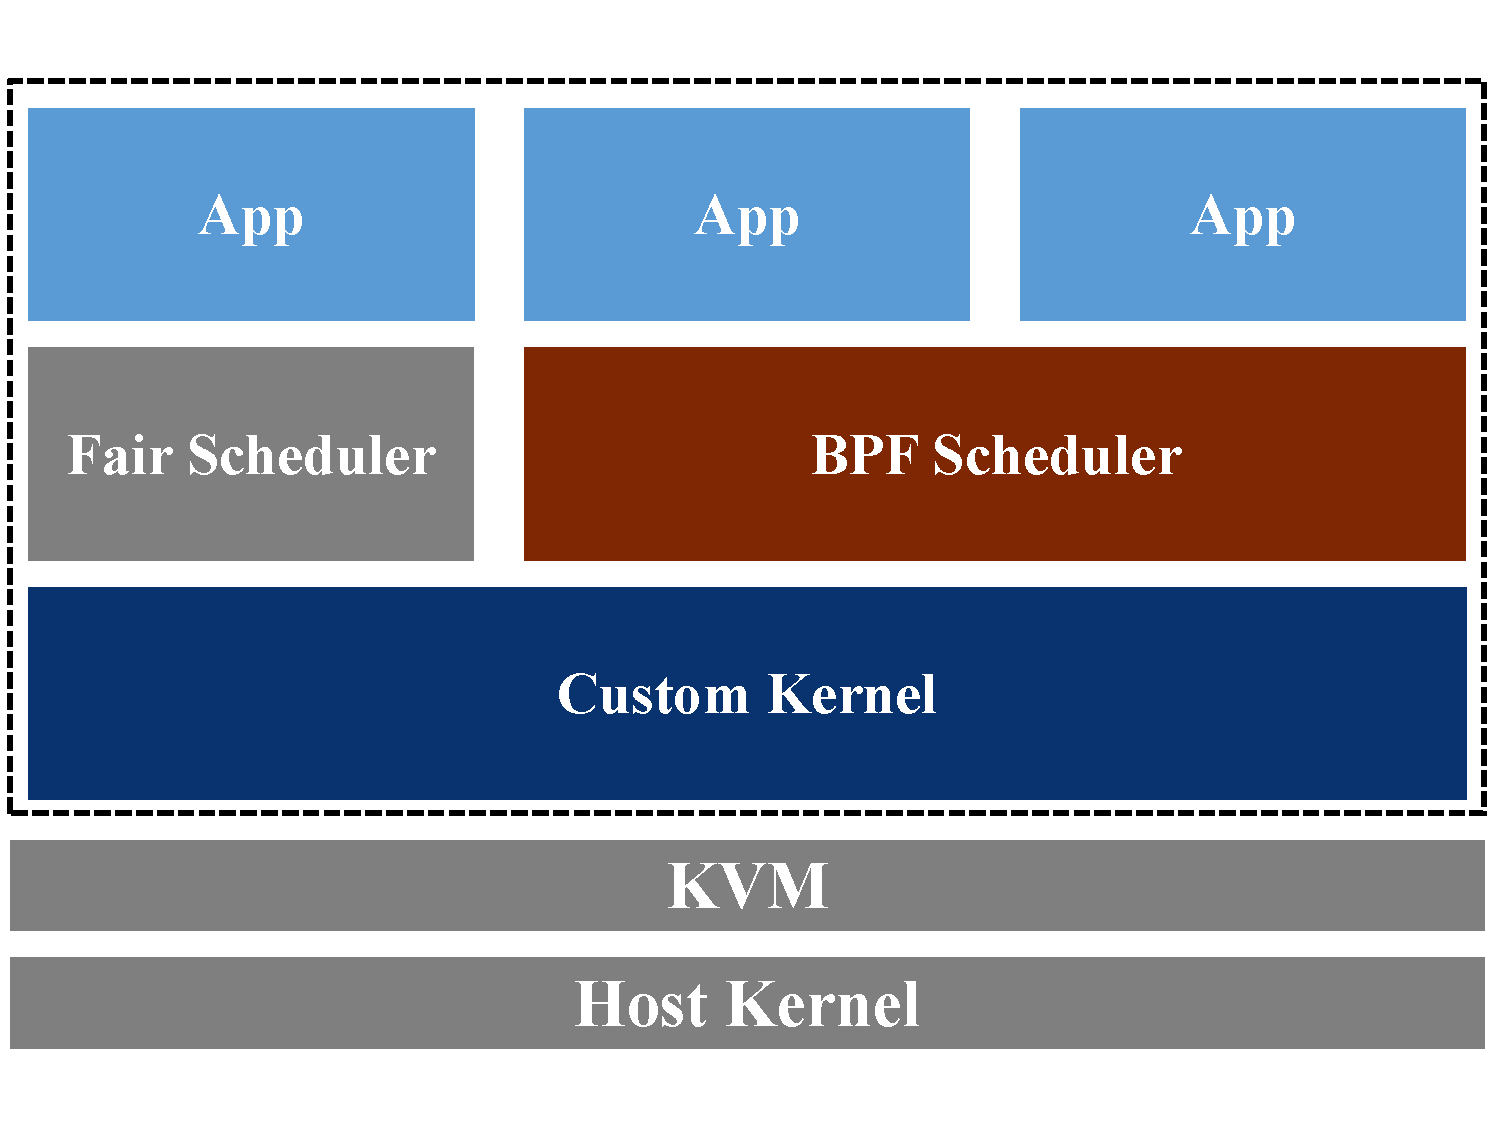
\includegraphics[width=\textwidth]{arch_dif_cz}
        \caption{Control Zone}
        \label{fig:arch_dif_cz}
    \end{subfigure}
    \hspace{0.5cm}
    \begin{subfigure}[b]{0.4\textwidth}
        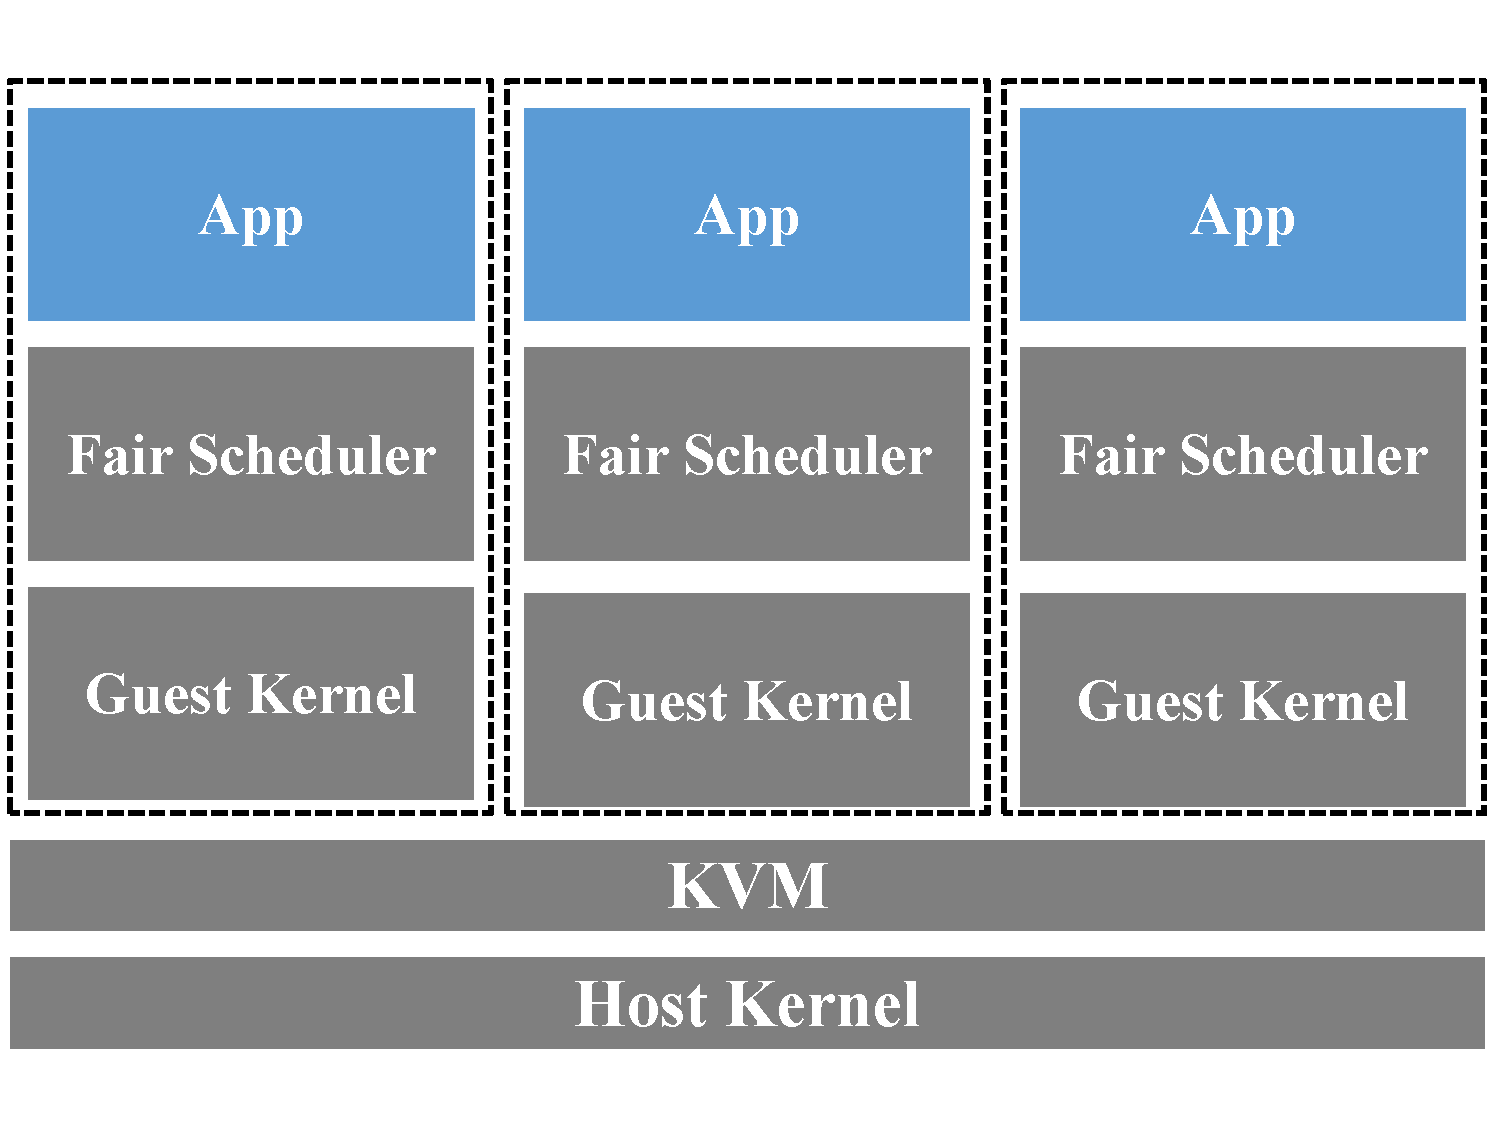
\includegraphics[width=\textwidth]{arch_dif_fc}
        \caption{Firecracker}
        \label{fig:arch_dif_fc}
    \end{subfigure}
\bicaption{\quad 沙箱结构差异}{\quad Sandbox Structure Differences}
\label{fig:arch_dif}
\end{figure}

\section{论文结构安排}

本文的主要内容分为六章,总体结构如图~\ref{fig:paper_organization}所示:

\begin{figure}[!htbp]
    \centering
    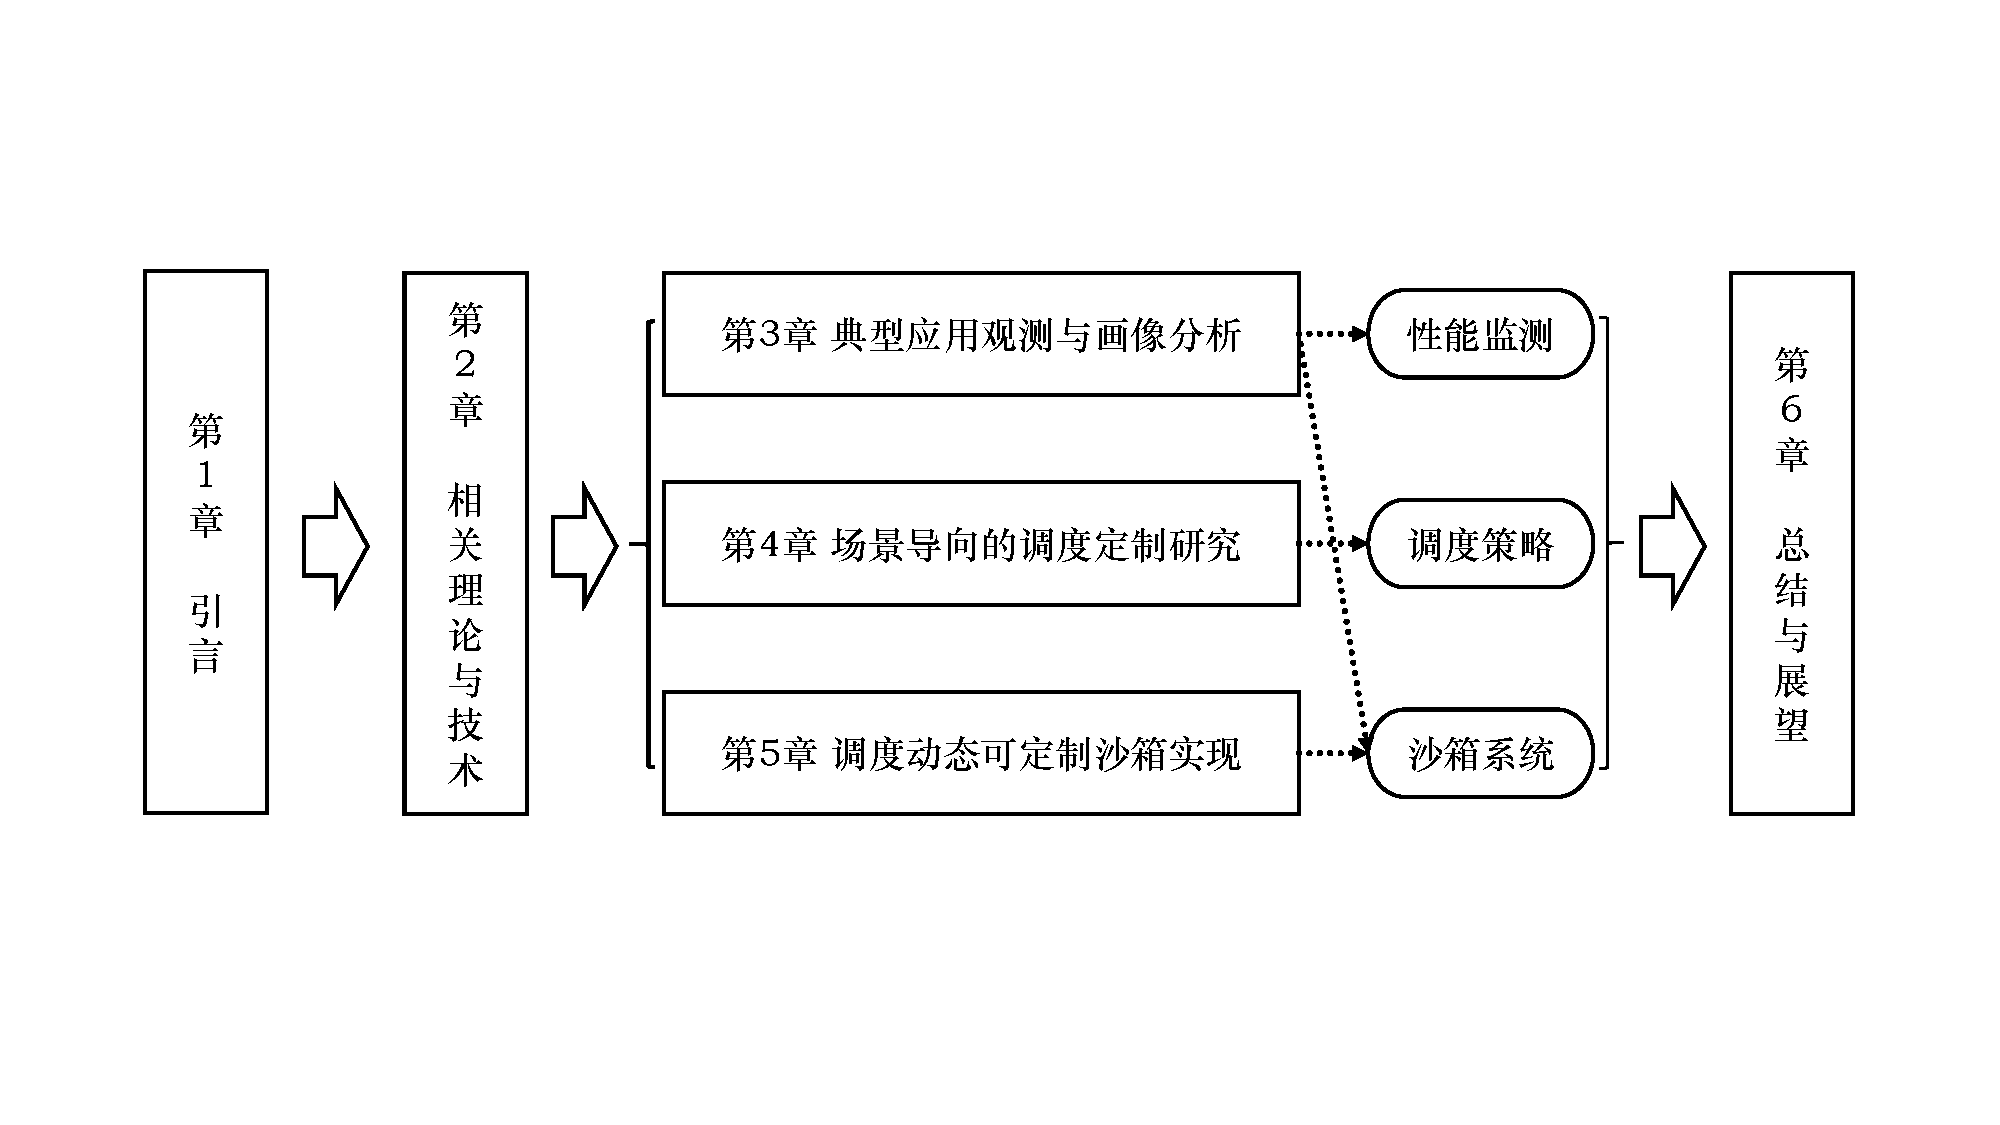
\includegraphics[width=0.8\textwidth]{paper_organization}
    \bicaption{\quad 本文组织架构}{\quad Paper Organization}
    \label{fig:paper_organization}
\end{figure}

第1章,相关背景说明。首先,阐述了本文的主要背景,以及面向混部场景的QoS保障问题。随后,从可观测性与劣化监测、围绕资源隔离的混部场景QoS保障、围绕任务调度的混部场景QoS保障三个方面分析了国内外研究现状。最后,阐述了本文研究所面临的挑战以及要展开的各项工作。

第2章,本文中所使用到的技术说明。首先,分析了经典的Linux调度子系统的构成以及任务调度的决策过程。其次,介绍了本文中使用到的eBPF技术,阐述其核心特点,以及相较于内核模块等传统内核功能扩展技术的差异。随后,介绍了Sched Ext项目,一种插件化内核调度器补丁集,说明了其实现的原理。最后,介绍了沙箱技术以及相关的实现。

第3章,典型应用观测与画像分析。首先,介绍了云场景典型应用以及应用运行环境的选择。其次,阐述了针对KVM虚拟机的多维度指标采集Black Box观测系统的设计与实现。最后,分别对基准性能实验与干扰敏感度实验进行实验设计的阐述与最后的画像结果分析。

第4章,混部场景导向的任务调度机制定制,包含内核配置定制、Control Tower任务调度框架两个方面。在内核调度配置上,设计了响应度优先与吞吐量优先两种内核配置。在Control Tower任务调度框架上,首先阐述了设计目标和实现原理,以及CPU资源感知与网络资源感知两种调度策略的实现。最后,设计实验验证场景导向的调度机制在应用QoS保障上的效果。

第5章,Control Zone的设计与实现。在第3、4章的基础上,设计实现了一种调度动态可定制沙箱。一方面能够通过内核调度定制与Control Tower任务调度框架,针对混部场景选择合适的任务调度机制。另一方面基于虚拟化,实现不同调度机制在同一物理机上共存。最后,设计实验说明沙箱的开销以及在混部场景下保障应用QoS的效果。

第6章,总结与展望。首先对于本文针对混部场景QoS保障问题的三个工作进行总结,分析了本文工作的效果与不足之处。随后,对利用eBPF观测能力与Ext调度类灵活性在更多混部场景定制Control Tower调度策略进行了展望。
\chapter{相关理论与技术}\label{chap:theories_tech}

% \section{可观测性}

\section{BPF技术}

eBPF(Extended Berkeley Packet Filter)是Linux内核中的一个轻量级、快速的64位的类RISC虚拟机\citep{sharaf2022extended}。当前eBPF当前已经成为在Linux内核运行时执行不可信的、由用户定义的专用代码的最佳实践与事实标准。其强大的性能、可移植性、灵活性与安全性得到了工业界和学术界的认可,并被广泛地用于更多的领域。

eBPF的前身是BPF(Berkeley Packet Filter),最早由McCanne和Jacobson设计并提出\citep{mccanne1993bsd},起初BPF如其名称所示,用于在Linux网络子系统中对网络包进行灵活处理,而因其本身优异的设计,被Linux内核社区的贡献者扩展到内核的各个子系统中,来对内核功能进行定制化,为了与旧BPF技术进行区分,内核社区将早期的BPF技术成为cBPF(Classic Berkeley Packet Filter),而BPF和eBPF均指代最新的BPF技术,本文在后续说明中也采用这种做法。

BPF本身是一种指令集,最初设计时考虑到安全性与易用性,允许开发者使用C语言的子集进行编写,并能作为一种编译器后端指令集,由GCC等常用编译器编译为字节码\citep{ebpfguidence}。BPF采用字节码的处于两种原因,其一是方便内核验证器对代码进行验证,其二则与Java思想类似,即利用字节码与语言虚拟机的组合提升可移植性。BPF虚拟机运行在内核中,Linux提供了相关的BPF系统调用来将字节码加载到内核中,并附加到代码中声明的钩子函数处,当对应函数触发时,内核态的BPF虚拟机就会执行附加的BPF字节码。整个过程中为了防止加载非法代码,内核首先会在加载BPF代码前对BPF字节码进行验证,判断是否符合在内核中执行的规范,如不允许死循环等,而在内核BPF虚拟机中执行时,会利用JIT技术将字节码映射到本机机器码,从而实现最佳的运行性能。

同作为对内核功能的扩展,BPF技术经常会与内核模块进行比较。相较于内核模块,BPF技术具有更高的安全性,BPF程序安全性体现在三个方面。首先不同于内核模块,BPF程序在编写时所有的对内核数据、地址的访问都需要通过BPF Helper函数来实现,同时,部分BPF Helper函数设计时就考虑到并发性,极大减少了不安全代码的数量。其次,BPF代码在加载时会被内核验证,同时由于运行在虚拟机中,也增强了安全性。最后,BPF代码所能执行的位置由内核提供,这样也大大缩小了危险代码的影响范围。

\begin{figure}[!htbp]
    \centering
    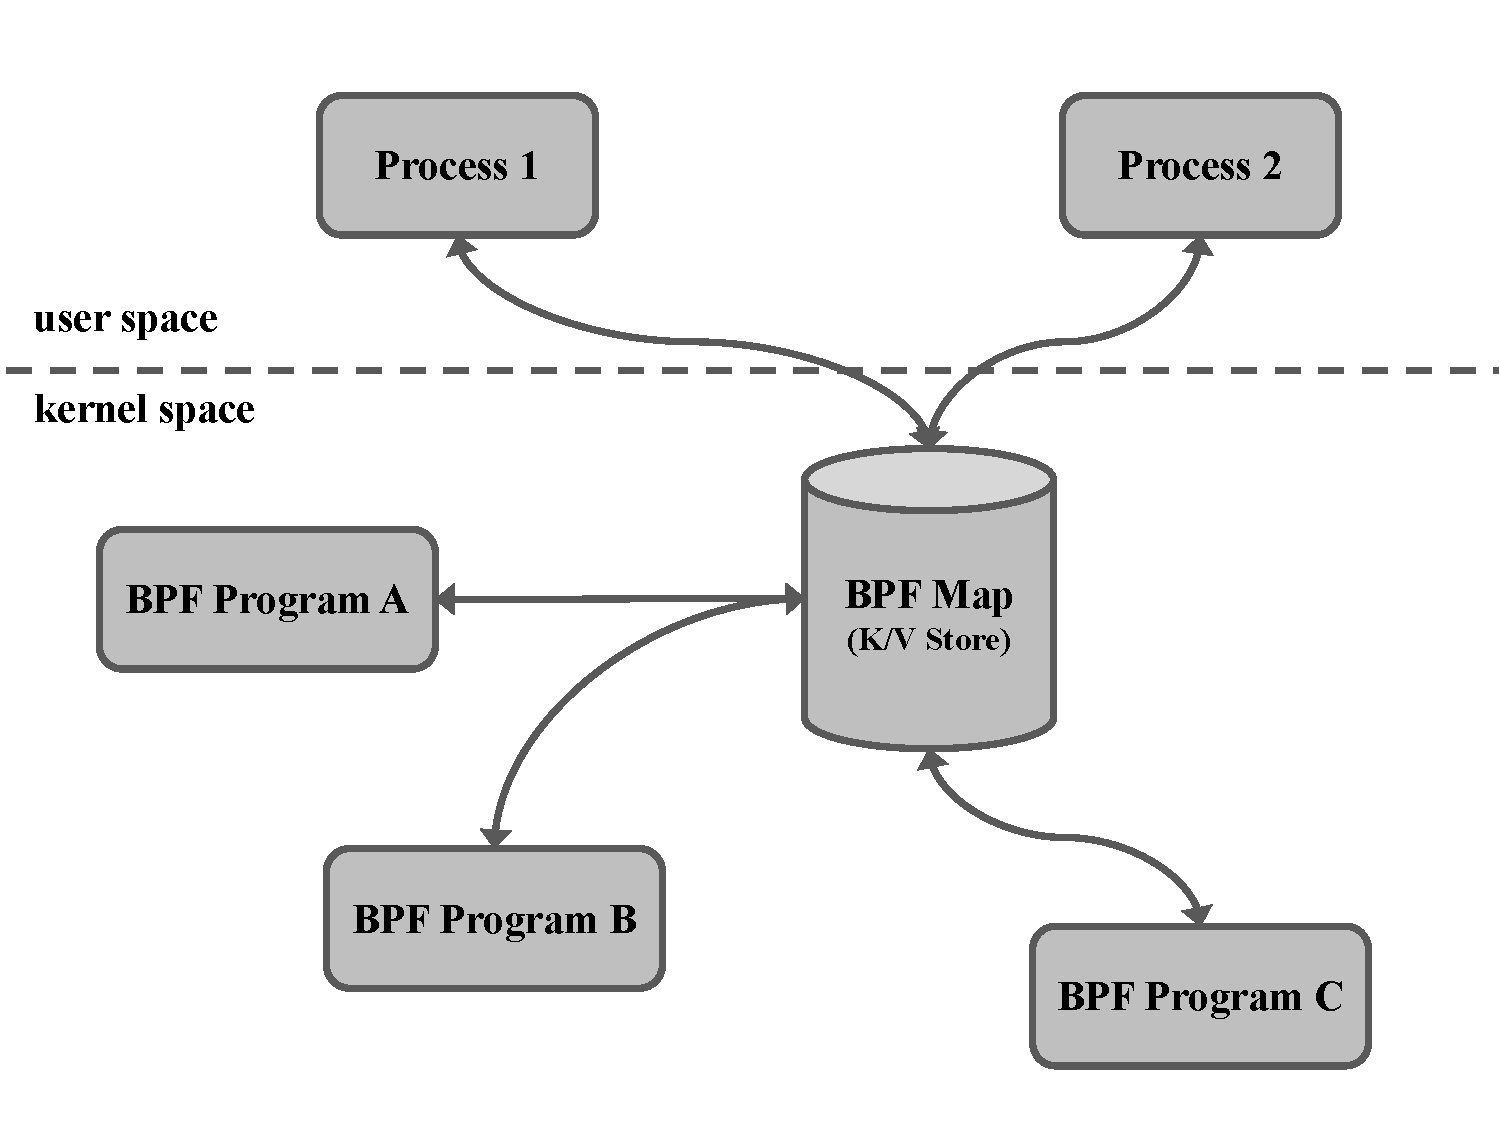
\includegraphics[width=0.6\textwidth]{bpf_user_kernel}
    \bicaption{\quad BPF中用户态与内核态的交互}{\quad Interaction between user mode and kernel mode in BPF}
    \label{fig:bpf_user_kernel}
\end{figure}

同时,BPF技术也具备高度的灵活性。这种灵活性体现在两个方面,首先对于用户态与内核态的交互,BPF技术运行由用户态的程序来加载BPF代码,由于BPF本身是字节码,因此能够借助libbpf等工具来对代码中的部分进行修改,这大大增强了BPF代码的灵活性。其次,如图~\ref{fig:bpf_user_kernel}所示,BPF技术允许通过BPF Map来实现用户态与内核的逻辑交互,一方面,内核态BPF程序所收集到的数据,能够借助BPF Map反馈给用户态程序进行处理,另一方面用户态程序也能通过BPF系统调用操作内BPF Map,对其中的内容进行读写,从而影响内核态BPF程序的行为。其次,BPF技术还允许BPF程序之间的交互,除上述通过BPF Map的交互外,如图~\ref{fig:bpf_to_bpf}所示,BPF程序还能够相互进行调用,从而进行数据传递,或通过多个BPF程序的调用,来突破内核对单个BPF函数的限制,从而实现更加复杂的代码逻辑。

\begin{figure}[!htbp]
    \centering
    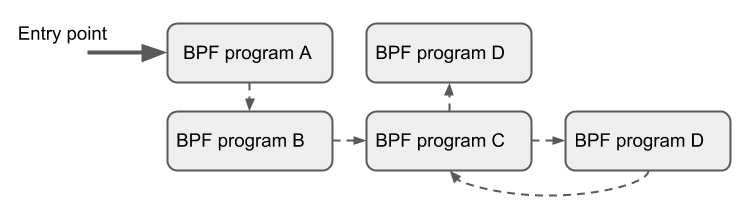
\includegraphics[width=0.7\textwidth]{bpf_to_bpf}
    \bicaption{\quad BPF程序之间的调用}{\quad Interaction between BPF programs}
    \label{fig:bpf_to_bpf}
\end{figure}

然而BPF技术也存在设计上的不足。由于在设计时首要考虑的是安全性,因此BPF程序在编写受到了种种限制,实际上,编写BPF程序所能使用的C语言子集是非图灵完备的,同时BPF程序在栈空间上也有严格的要求。这些限制都极大削弱了BPF程序的表达能力,使得其能够编写的逻辑十分有限。内核社区关注到这一点,并在近期的版本更新中逐步地减少对BPF程序的限制。

\section{Sched Ext}

Sched Ext是一种可扩展的内核调度器设计\citep{schedext},由Meta以及内核社区的工程师共同设计实现,并已经在Meta的集群中运行与测试。Sched Ext最早提出于2022年,当前尚未合并入内核主线,但Meta与内核社区开发者十分活跃,Sched Ext当前仍然正在积极更新并持续地向内核社区提交Patch。

Sched Ext启发自ghOSt\citep{humphries2021ghost},其同样考虑到内核调度器在开发与部署上的困难,与当前数据中心对于定制调度器的需求的不匹配,因此以设计一种插件化的调度器,来提升内核调度器开发的灵活性。然而不同于ghOSt,Sched Ext在设计初就尽可能地保持与Linux现有调度就机制的兼容性,这点在Sched Ext调度类的优先级上就有所体现,如图~\ref{fig:sched_ext_priorty}所示,开发者有意将Sched Ext调度类的优先级定义在Sched Normal之下,这就使得常规应用仍然可以由Sched Normal处理,从而最大地与当前Linux的调度机制兼容。

\begin{figure}[!htbp]
    \centering
    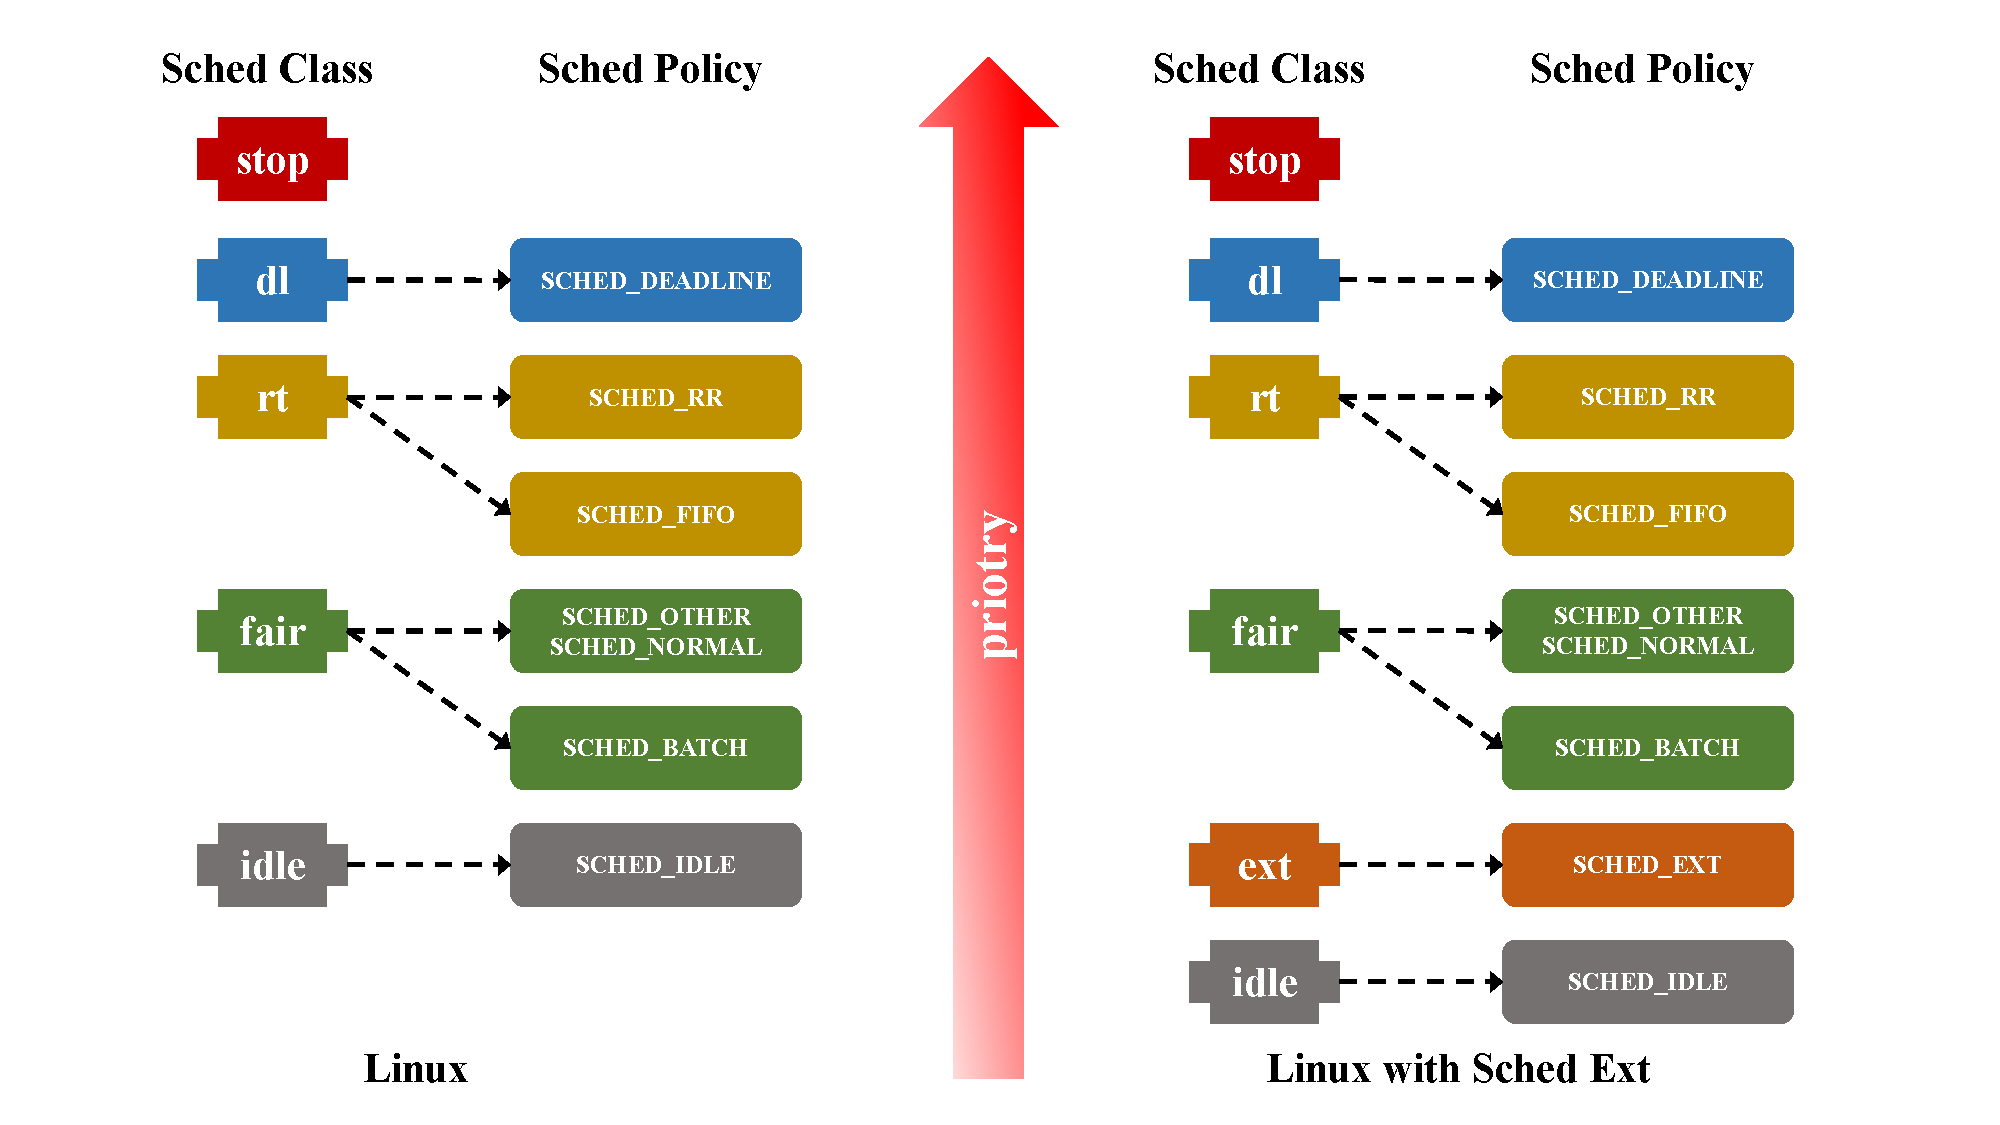
\includegraphics[width=0.7\textwidth]{sched_ext_priorty}
    \bicaption{\quad Sched Ext 调度优先级}{\quad Sched Ext Priorty}
    \label{fig:sched_ext_priorty}
\end{figure}

Sched Ext调度类实现了所有调度类方法,但是在每个方法的实现中,仅进行了函数开头的设置与结尾时资源的回收,所有调度相关的核心实现都依赖BPF函数中的实现:

1)enqueue_task,当一个任务需要被加入到调度器的就绪队列时被调用,从而将进程加入到就绪队列,准备进行调度。

2)dequeue_task,当一个任务不再需要调度(如被挂起或完成)时被调用,从就绪队列中移除进程。

3)yield_task,当一个任务主动放弃CPU时间时,通常是在执行了yield系统调用后被调用,从而允许其他进程使用当前未使用的时间片。

4)check_preempt_curr,在每次任务唤醒时检查是否需要抢占当前运行的任务,从而确定当前运行的任务是否应该被新唤醒的任务抢占。

5)pick_next_task,选择下一个要运行的任务,一般从就绪队列中选择下一个要执行的任务。

6)put_prev_task,当前运行的任务停止运行时被调用,通常需要更新该任务的调度信息,并在其还有继续运行时放回就绪队列。

7)set_curr_task,每次切换到新任务时被调用,通常用于更新调度器的指示当前任务的curr指针。

8)task_tick,每次系统时钟中断发生时被调用,一般时更新当前任务的调度信息,同时也包括当任务时间片使用完时执行抢占。

9)task_fork,当一个新的任务被创建(fork)时被调用,通常用于处理新任务的调度相关设置。

10)task_dead,当一个任务彻底结束并且要被移除时被调用,用于清理该任务的调度相关资源。


\begin{figure}[!htbp]
    \centering
    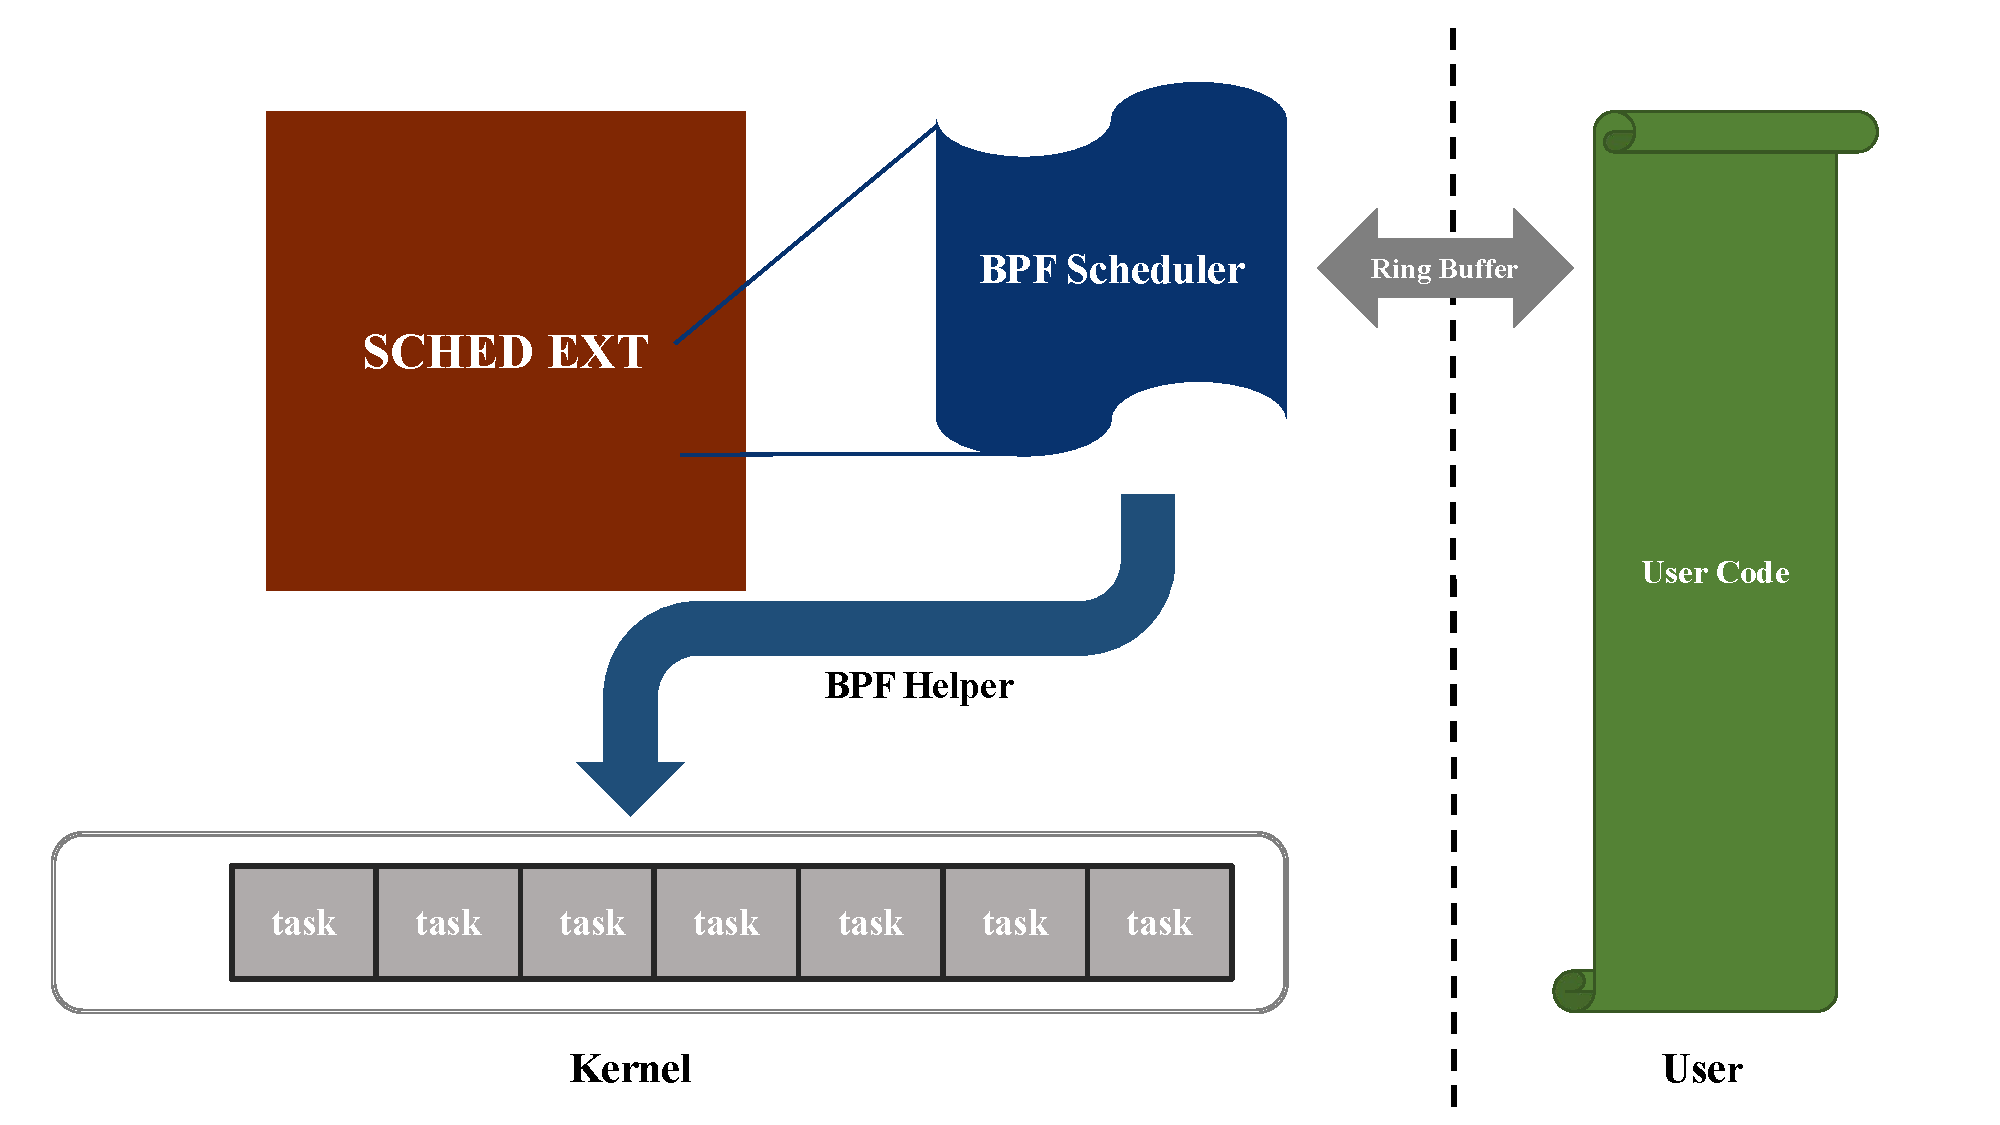
\includegraphics[width=0.7\textwidth]{sched_ext_arch}
    \bicaption{\quad Sched Ext架构}{\quad Sched Ext Arch}
    \label{fig:sched_ext_arch}
\end{figure}

如图~\ref{fig:sched_ext_arch}所示,Sched Ext基于BPF的可编程设计提供了丰富的手段来定制化调度过程。首先最直接的就是通过BPF代码定制调度逻辑,,这种方式的好处就在于所有的调度过程仍然在内核中进行,因此不会有用户态与内核态频繁切换的开销,而开发者仅需要提交BPF代码。其次,开发者可以直接操作任务队列来控制调度过程,Sched Ext将调度中核心的任务队列暴漏了出来,并允许通过BPF Help函数直接操作任务队列,这使得在调度程序完全能够在用户态进行实现,同时Sched Ext还提供了基于C与Rust语言的库函数,方便了开发者进行调度器设计,这种方式虽然引入了地址空间切换的开销,但也极大增加了调度器设计的灵活性。

默认情况下仅由Sched Ext类的任务会被BPF调度程序处理,而如果BPF调度程序尚未加载,Sched Ext调度类的任务仍然会交给Sched Normal进行处理,以避免任务得不到执行。同时,Sched Ext还允许通过特殊的BPF Helper函数,将SCHED NORMAL即以下的任务全部交给SCHED EXT进行处理,这种情况下,Sched Ext调度类就能够参与系统中核心的调度过程。

\section{本章小结}

本章主要介绍了eBPF技术以及Sched Ext可扩展内核调度机制。其中eBPF技术提供了一种集性能、灵活性于安全性于一体的扩展内核方式,利用eBPF技术能够方便地从内核中获取更多细致的数据,同时也能够在一些支持相对丰富的内核子系统中对内核功能进行定制。而Sched Ext提供了一种内核主线之外扩展内核调度的方式,其本身基于eBPF技术,因而能够利用到eBPF本身所具备的优势,同时其在调度子系统中展开了许多工作,使得通过eBPF程序定制调度逻辑成为可能,而其在设计上对于兼容性的考量,也方便了其在生产环境中的部署于测试。如上技术为本论文对应用进行细粒度监控,构造Control Zone与为不同混部场景设计不同的调度策略奠定了基础。


\chapter{典型应用观测与画像分析}\label{chap:profiling}

\section{云场景典型应用选择}

% 软件环境复杂 -> 应用需求不同 -> 软件架构复杂 -> 存在共性的基础应用 -> 基础应用的性能是整体性能的关键 -> 选取典型应用进行分析

数据中心软件环境复杂,同时托管的应用种类较为丰富,为画像分析带来了许多挑战。首先,数据中需要根据用户的使用需求,提供不同的软件环境,如针对虚拟机,需要提供虚拟化环境,而对于容器,则需要提供如K8s等,本研究结合与云厂商的合作经验,选择云场景中使用较普遍的虚拟机作为目标场景,在该场景中,应用的运行环境由宿主机系统、虚拟化运行时及Guest操作系统共同完成。其次,数据中心托管应用丰富的主要原因是需求的差异,然而当前随软件架构的不断进步及开源、云原生等理念的推广,应用在设计时会使用到许多相同的公共组件,如数据库、消息中间件等,这些公共组件构成了现代软件的基石,同时也是应用性能的关键,因此在本研究中,结合与云厂商的合作经验,从传统数据库、键值存储、消息中间件、大数据、媒体处理等领域中选择了如表~\ref{tab:typical_application}所示的7种典型应用进行画像分析。

\begin{table}
    \bicaption{\quad 云场景典型应用}{\quad Typical Applications in Cloud Scenarios}% caption
    \label{tab:typical_application}
    \footnotesize% fontsize
    \setlength{\tabcolsep}{4pt}% column separation
    \renewcommand{\arraystretch}{1.5}% row space 
    \centering
    \begin{tabular}{lc}
        \hline
        %\multicolumn{num_of_cols_to_merge}{alignment}{contents} \\
        %\cline{i-j}% partial hline from column i to column j
        类型 & 应用\\
        \hline
        SQL & mysql\\
        NoSQL & elasticsearch\\
        Web Server & nginx\\
        K-V Store & redis、memcached\\
        Message Queue & kafka\\
        Media & render\\
        \hline
    \end{tabular}
\end{table}

这些应用在领域上的差异,决定了其在功能实现上的不同,并会使用到不同的资源,因此各自对调度有不同的需求:

1)数据库类型的应用,如Mysql,传统的关系型数据库提供了完善了数据存储、检索查询及事务管理等功能,实现中原始数据通常保存在磁盘上,在进行大量数据查询时,不仅会使用到较多的CPU资源,同时也会占用相当的IO资源,因此需要调度器保障其CPU资源,并避免IO上的干扰。

2)键值存储类应用,如Redis、Memcached,通常作为信息缓存服务,提供快速的数据存储与查询,由于数据存储在内存中,因此对内存资源存在较高要求,对调度的需求主要体现在两方面,一方面需要足够的内存资源,另一方面则需要避免在内存带宽上的干扰。

3)网络服务类型应用,如Nginx,网络页面通常都具有交互属性,而延迟会极大影响用户的使用体验,因此这类应用要求调度能够在网络请求到达时,及时的为网络服务分配CPU,以尽早地对连接进行处理。

4)媒体处理应用,如ffmjpeg,通常是离线应用,运行时会占用大量的CPU资源,来进行编解码操作,这类应用需要调度分配足够长的时间片,同时希望能减少上下文地切换,以便更好地利用局部性来加快执行速度。

\section{观测系统设计与指标收集}

\subsection{面向虚拟机的多维指标采集设计}

% 分解虚拟机: Host侧 -> Hypervisor侧 -> 应用侧
% 分解采集系统:
% - 采集侧
% - 查询、存储、分析侧

本研究中使用KVM虚拟机作为混部应用基本软件环境。而结合第二章中对于虚拟化沙箱技术的分析,本研究设计了一种如图~\ref{fig:virtualmachine}所示的面向虚拟机的多维度指标采集机制。

\begin{figure}[!htbp]
    \centering
    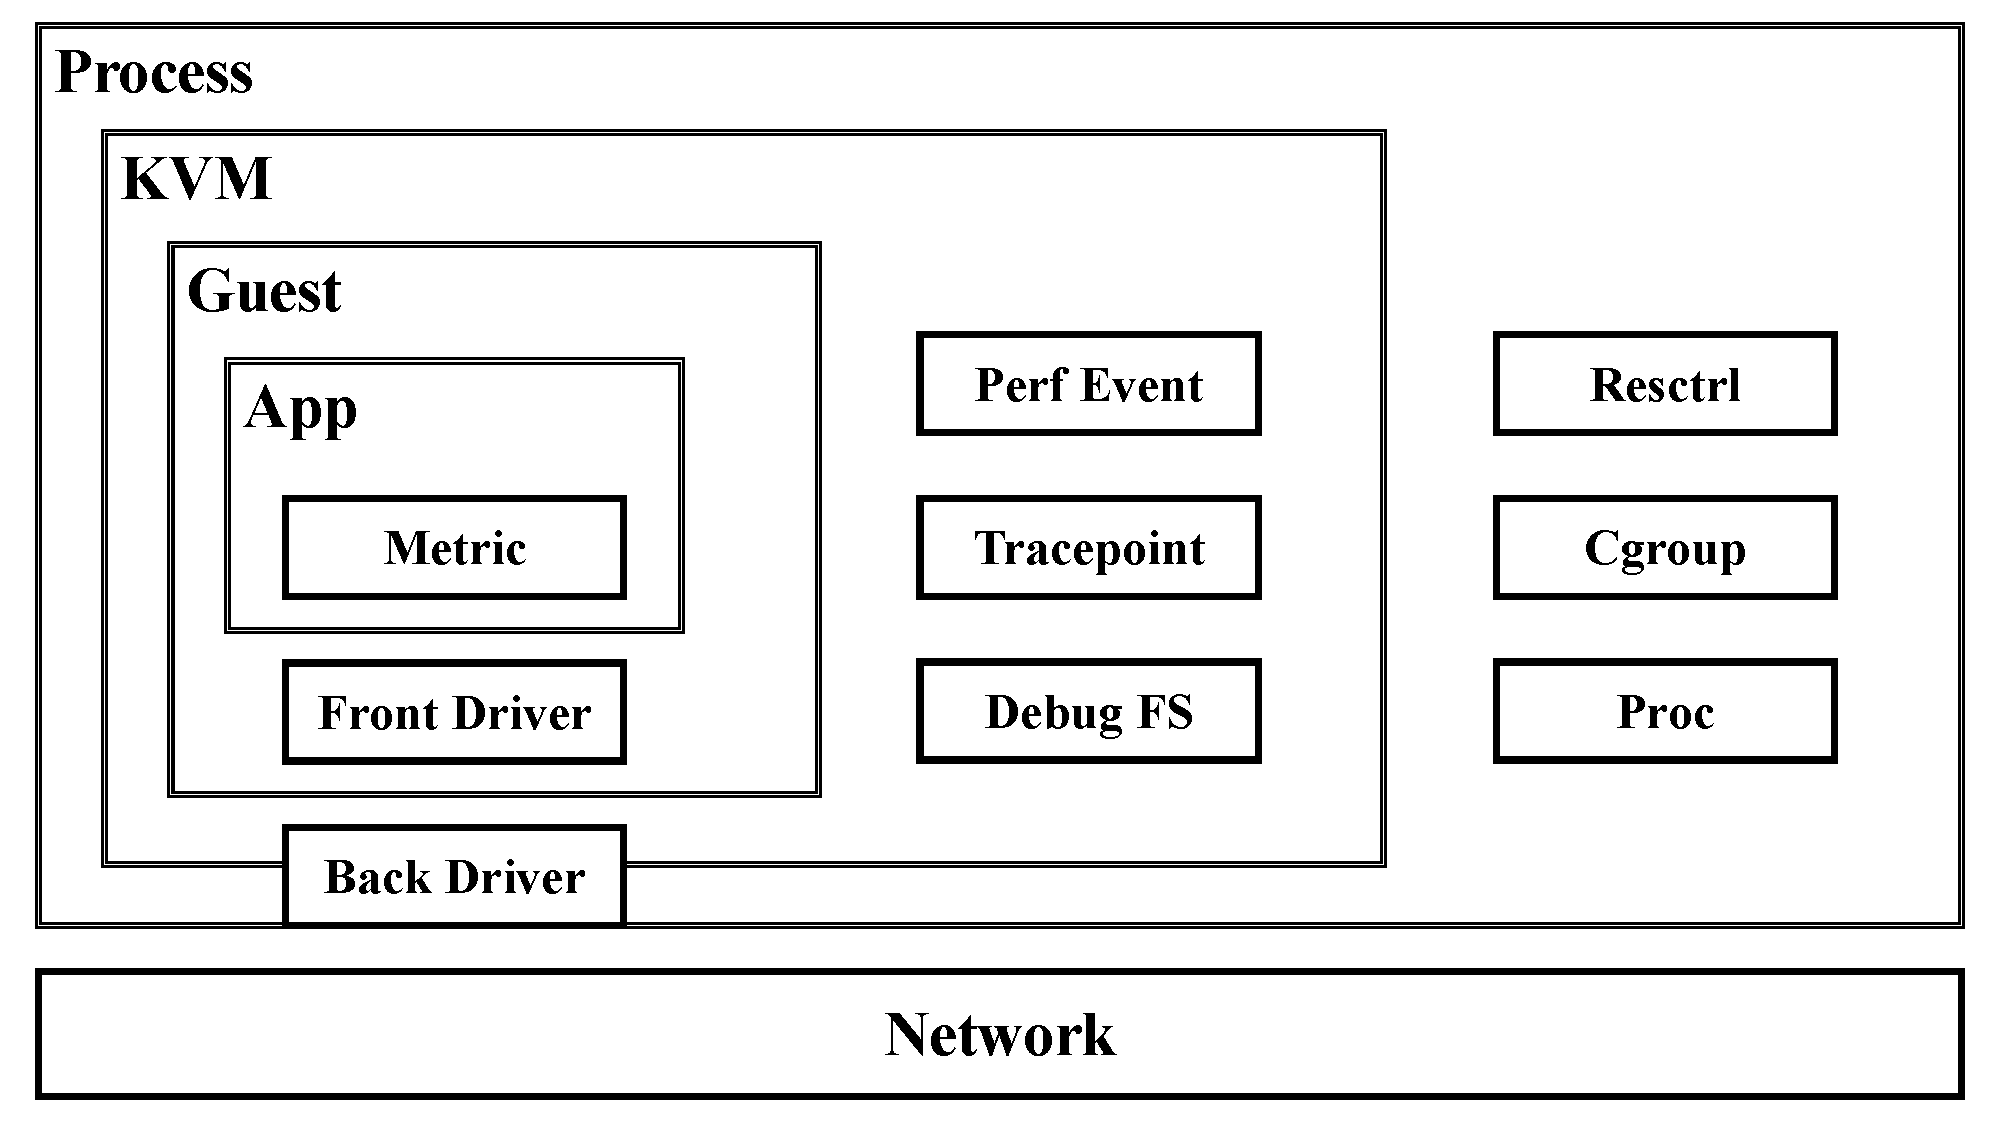
\includegraphics[width=0.7\textwidth]{virtualmachine}
    \bicaption{\quad 虚拟机多维度指标采集}{\quad Multi-dimensional metrics from virtual machines}
    \label{fig:virtualmachine}
\end{figure}

首先,在宿主机上,KVM虚拟机由多个进程组成,因此在这一维度,可以利用宿主机Kernel提供的多种进程监测机制,如/proc内核文件系统中记录的进程信息,以及cgroup子系统中对进程的记账信息,来评测虚拟机进程的性能。其次,虚拟机由各个模拟硬件组成,这些设备由Hypervisor进行模拟,在此维度,能够利用Hypervisor提供的丰富接口,来获取虚拟机的各个虚拟机设备的性能信息,以vCPU为例,本研究中KVM内核模块负责虚拟机的vCPU模拟,而KVM内核模块通过debug文件系统提供了丰富的vCPU监测信息,如包括IO、挂起、中断等在内的陷出计数,以及MMU缓存缺失计数等。最后,虚拟化环境最终需要为应用的运行提供服务,应用级指标能够体现出应用的真实性能,而针对这一维度的指标采集,主要从两个方面入手,对于Client-Server类的服务型应用,可以在外部通过Overlay网络建立对延迟、吞吐量的追踪,部分应用也内置了观测接口,提供性能信息的采集。

而为更深入地探测虚拟机性能,本研究还基于eBPF设计了一种在内核侧监测的机制。首先,在宿主机维度,进程对于硬件资源的使用通常都需要通过系统调用完成, 如使用网络资源时,需要使用send或recv系统调用,使用IO资源时,需要进行read、write系统调用,对虚拟机而言,这种方式能够监测陷出到用户态之后的设备模拟过程。其次,在Hypervisor维度,为追求设备模拟的效率,一些模拟硬件的后端实现并不要求虚拟机陷出到用户态,而直接在内核态完成整个模拟过程,如图~\ref{fig:vhost_net}所示,vHost net作为一种内核态实现的模拟网络设备后端,其网络发送的过程就直接在内核中通过函数调用进行,而这些函数的执行状态能够反映出模拟网络设备后端的性能。

\begin{figure}[!htbp]
    \centering
    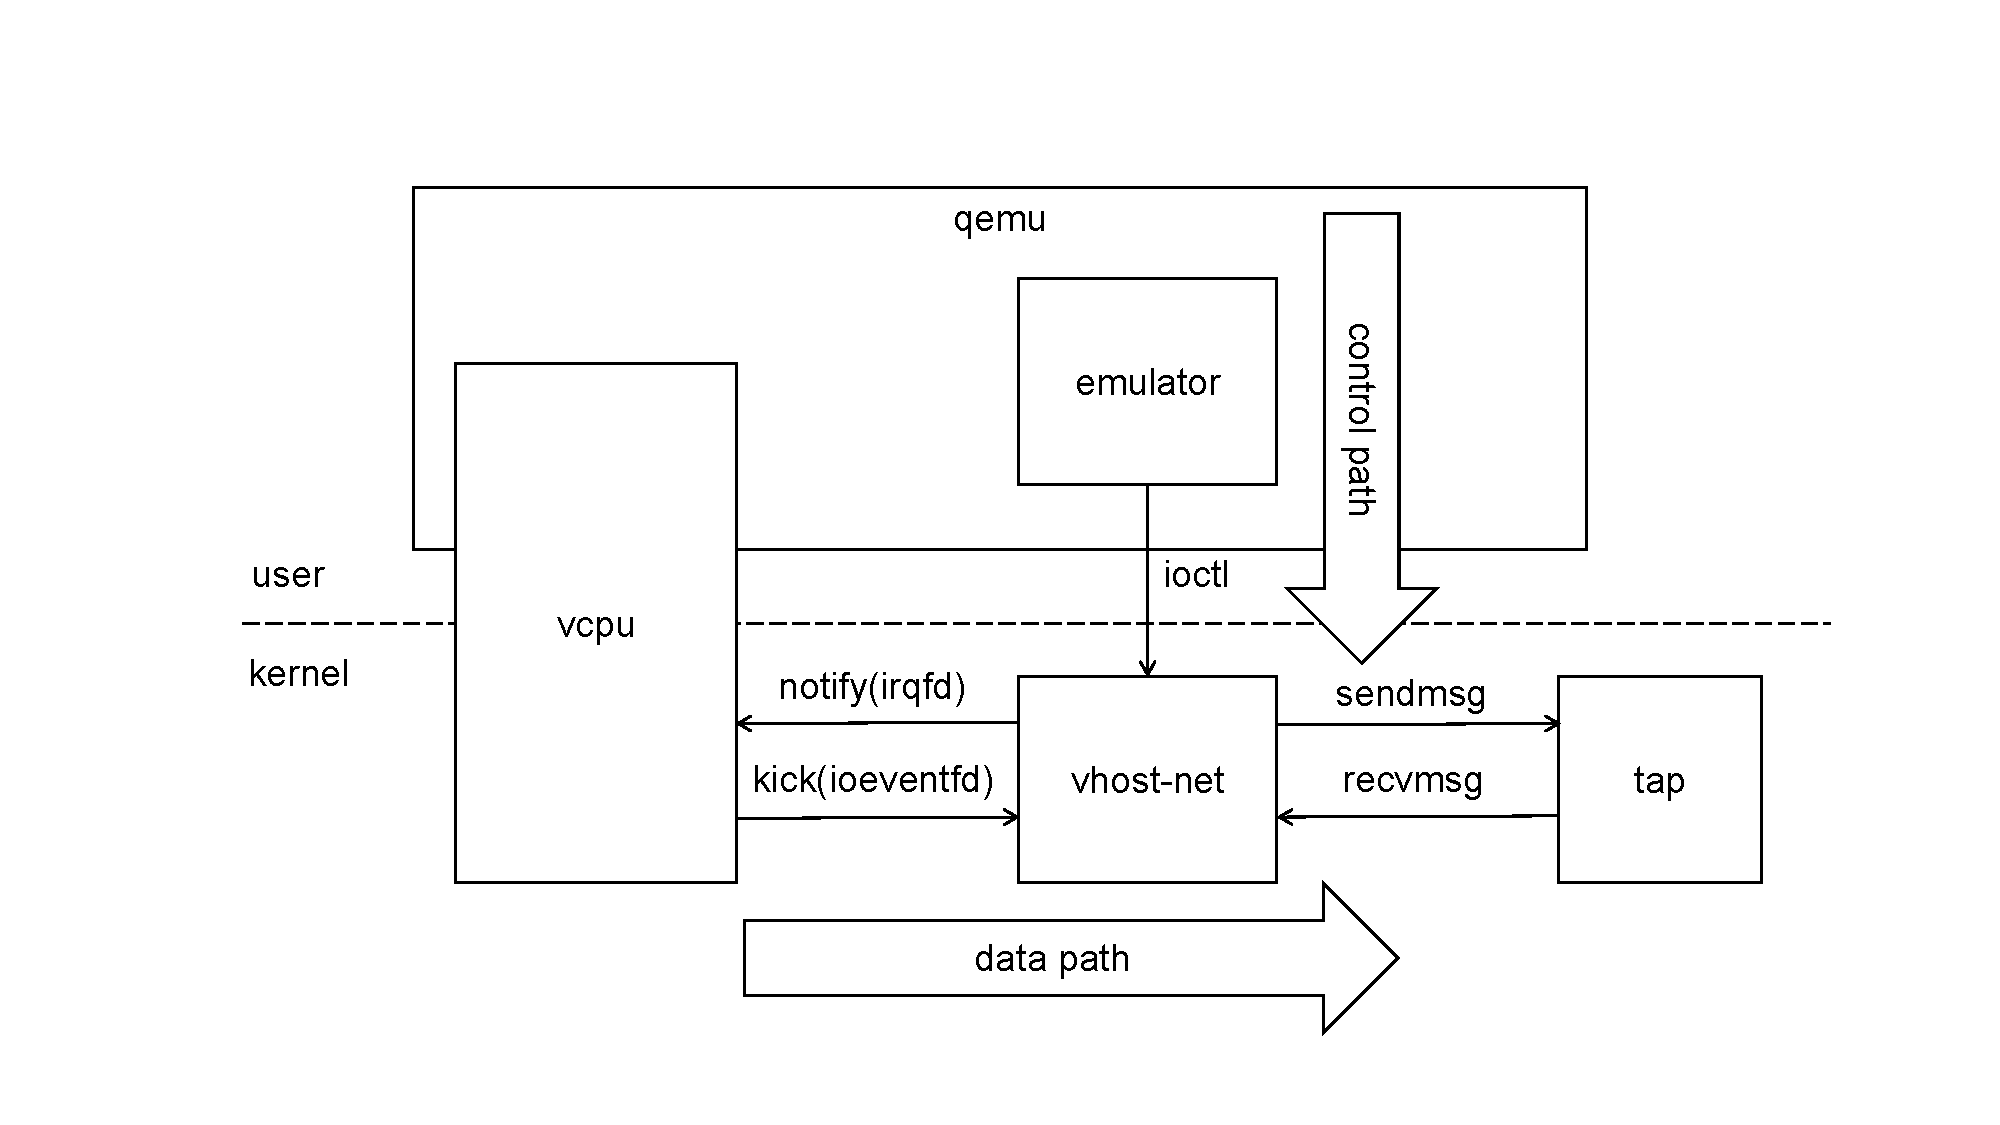
\includegraphics[width=0.7\textwidth]{vhost_net}
    \bicaption{\quad vHost Net模拟网络设备后端}{\quad vHost Net Simulate network device backend}
    \label{fig:vhost_net}
\end{figure}

综合以上分析,本研究设计了一种实时指标采集分析系统,能从上述维度以虚拟机为粒度机进行指标采集,同时能够提供指标的存储、查询与分析服务。系统中定义了Observer与Observed两种角色,首先,Observer与Observed以统一的格式对指标进行编解码,随后,Observed中部署监控组件以对外部提供监控服务,最后,Observer周期性地轮询各个Observed,并将收集到的原始指标按标签进行区分存储,并根据预定义的规则对指标进行聚合处理,同时对外提供查询与分析服务。系统中可以有多个Observer来分摊采集压力,并且每个节点可以按需要同时承担Observer与Observed两种角色。

\subsection{实时可观测性系统实现}

% Observer实现
% - Prometheus、Grafana、Collector Utils
% Observed实现
% - Exporter的实现细节
%   - Ebpf Exporter
%       - Syscall 追踪
%       - vHost Net 追踪

\begin{figure}[!htbp]
    \centering
    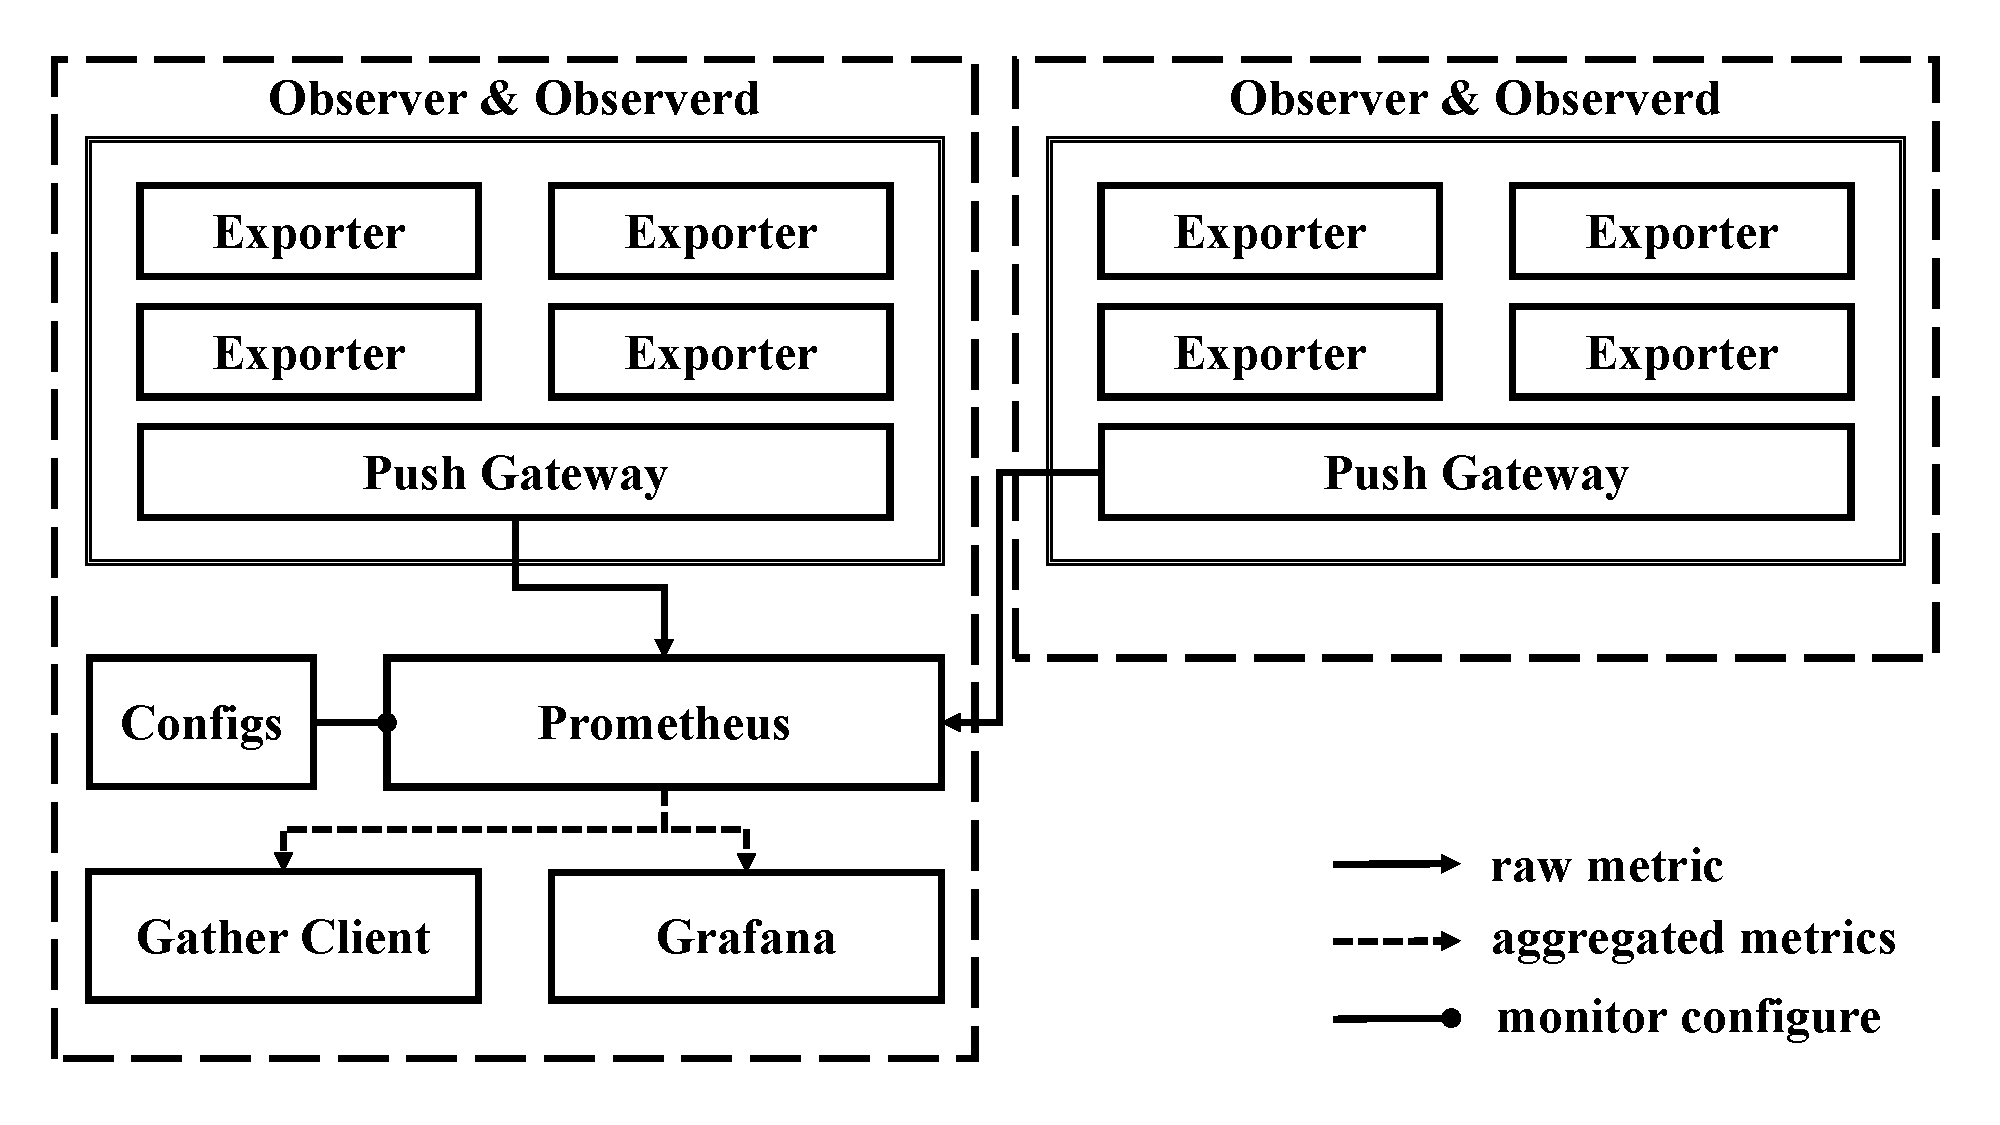
\includegraphics[width=0.8\textwidth]{monitor_arch}
    \bicaption{\quad 采集系统架构}{\quad Metric Collection System Architecture}
    \label{fig:monitor_arch}
\end{figure}

本研究结合云原生的实践经验,选择基于Prometheus来实现可观测性系统。Prometheus\citep{prometheus}是云厂商中广泛使用的一种指标监测系统,具有可扩展性强、灵活性好、生态丰富、部署便捷等特点,Prometheus的核心贡献在于提供了一种扩展性强的时序数据结构Metric以及围绕Metric的PromQL向量查询语言、向量数据存储方式以及编解码机制,在此基础上,Prometheus还实现了一套采集系统,提供了Promethues Server、Grafana及Node Exporter等核心组件,由于Promethues完全开源并提供了各种语言的Metric采集基础库,因此吸引了大量开发者及云厂商的参与,催生出丰富的组件生态。当前Prometheus已经成为指标采集的主要标准,并随DevOps的发展被越来越广泛地使用。

基于Prometheus生态的实时可观测性系统架构如图~\ref{fig:monitor_arch}所示,其中Observer的基于Prometheus Server与Grafana标准组件实现,在向量数据存储上,将原生的TiDB替换位InfluxDB,InfluDB使用以Rust语言编写,性能更强、扩展性更好。在采集上,Observer中虚拟机各维度数据的采集组织为一个服务发现配置文件,基于Prometheus的服务发现规则编写。而在数据聚合上,各维度原始数据首先需要进行初步处理以生成有效数据,Observer提供了PromQL编写了基本的聚合规则,实现对于标量数据的变化速率、99分位数据等的统计,同时这些规则会转化为Grafana中的Dashboard以进行实时监测。

可观测性系统中Observed的实现则包含了各个维度的Exporter的开发与配置。如图~\ref{fig:exporters}所示,Observed中包含了6种Exporter,能够在Host、Hypervisor、App三个维度围绕虚拟机提供丰富的数据采集,原始指标如表~\ref{tab:metric_list}所示,包含CPU、Cache、Memroy、IO、Network等各个子系统,总数量达到344个。

\begin{figure}[!htbp]
    \centering
    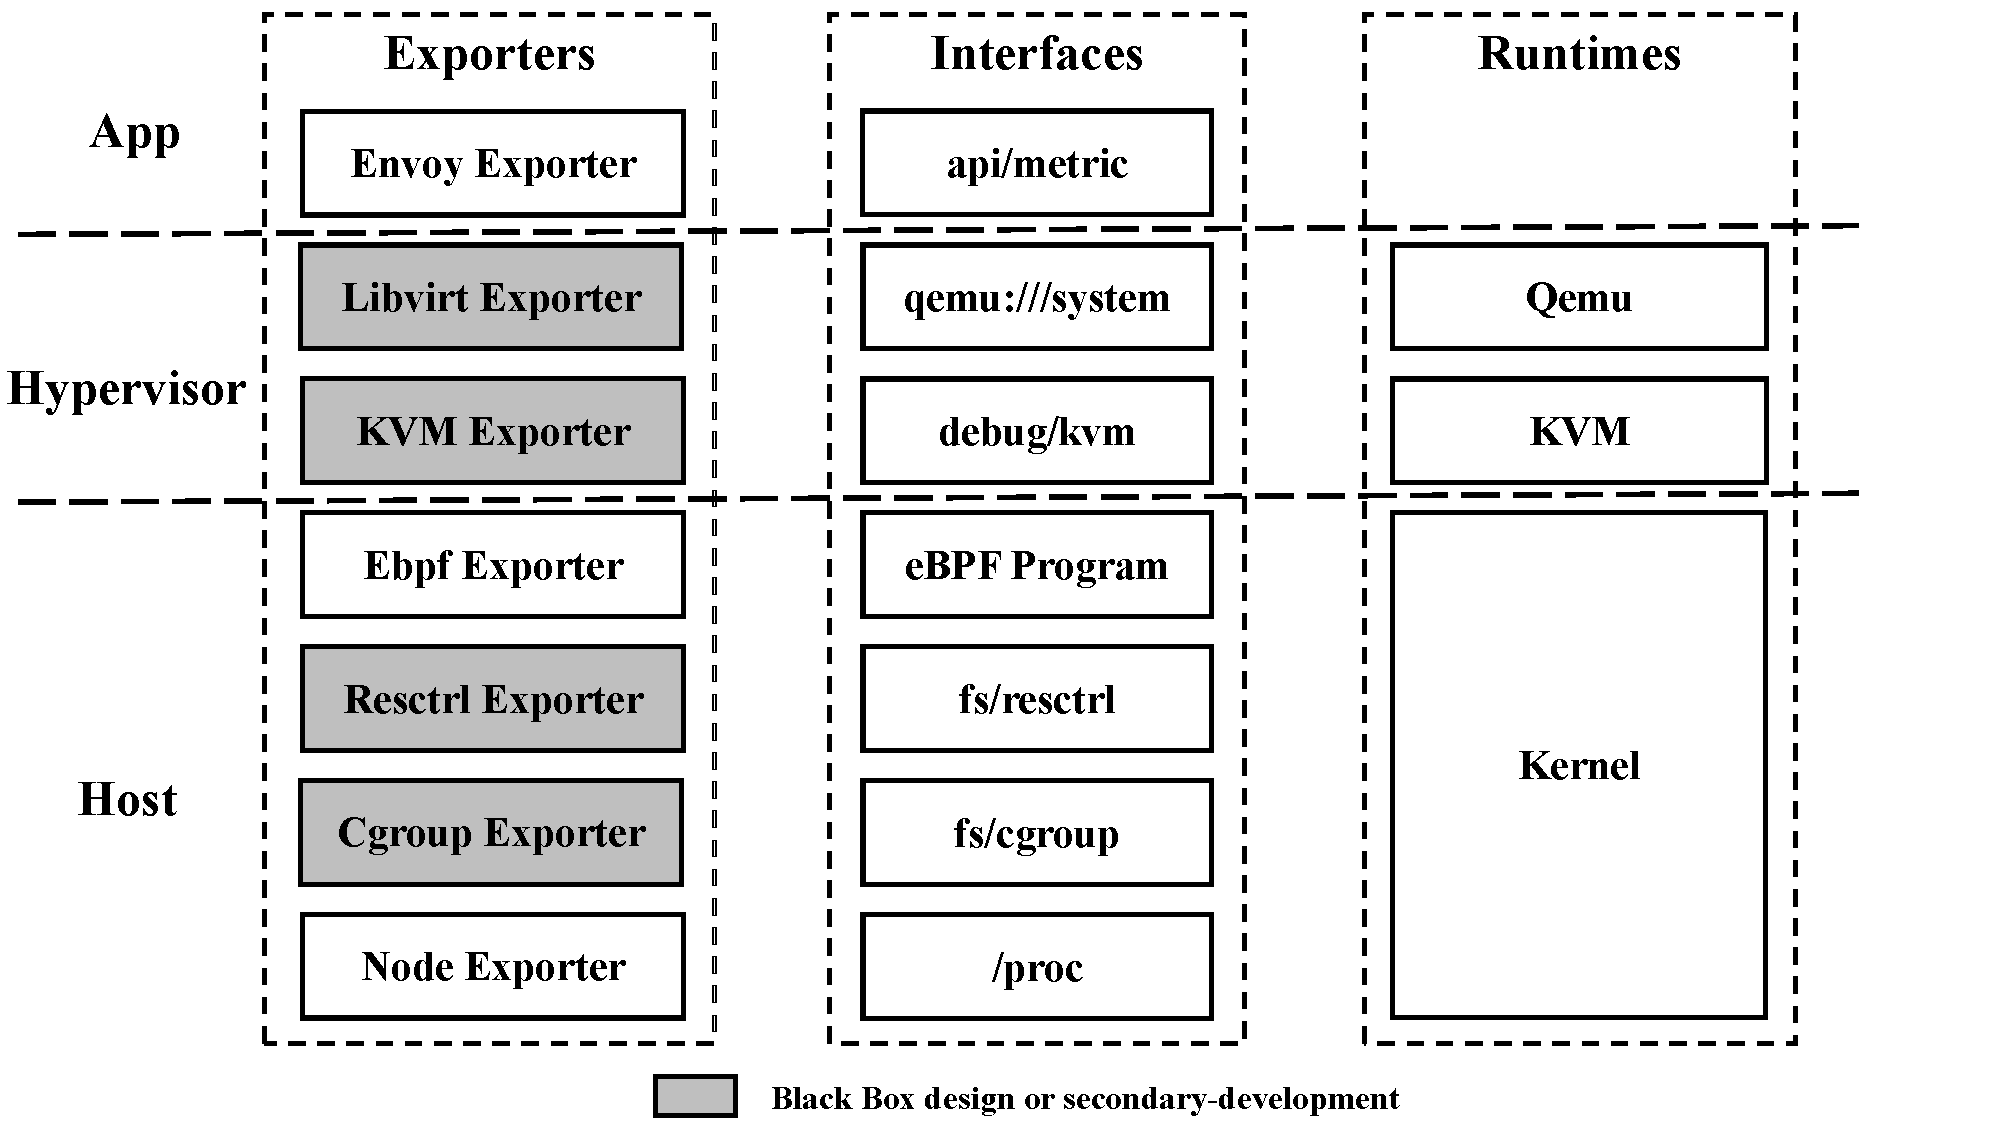
\includegraphics[width=0.9\textwidth]{exporters}
    \bicaption{\quad Exporters设计}{\quad Exporters Design}
    \label{fig:exporters} 
\end{figure}

1)Node Exporter是Prometheus提供的基础监控组件,提供Host维度的基础指标采集。其实现中主要利用了Linux Kernel提供的交互结果,来获取Host各个子系统中的运行状态信息,如通过/proc内核文件系统,获取运行时间、内存信息等。Observed实现中使能了NodeExporter的Perf Event监测模块,模块支持采集Host上的性能事件,包括cycles、instruction及cache miss等。

2)Resctrl Exporter实现了Resctrl子系统的指标采集。Intel RDT等硬件技术提供了进程粒度的CPU末级缓存与内存带宽的监测能力,Linux Resctrl作为这类技术的软件接口,提供了一个内核文件系统,用户可以通过在此文件系统中创建文件夹的形式来创建Monitor Group,而将进程加入到其中之后,Resctrl子系统就会开始为进程记录LLC与内存带宽信息。Resctrl Exporter基于Resctrl子系统实现, 通过扫描子系统中的Monitor Group来生成相关的指标信息,并将Monitor Group作为标签以便于后续聚合。

3)KVM Exporter实现了Hypervisor维度的指标采集。KVM内核模块提供了一个Debug文件系统,在最顶层的目录中,记录了内核模块的运行信息,如虚拟机陷出的总计数等,同时,对于每个虚拟机进程,还会创建对应的子目录,并以单个虚拟机为粒度记录内核模块的运行数据,最后,在每个虚拟机目录中,还会为每个vCPU创建一个目录,记录vCPU的时钟源相关信息。KVM Exporter基于上述机制实现,通过扫描Debug系统中的目录,并为遍历每个虚拟机条目来生成相关的指标信息,默认情况下使用虚拟机进程号作为标签,也允许传入一个配置文件,来实现虚拟机进程号与虚拟机名称之间的转化。

4)Libvirt Exporter是社区开发的一个监控组件,提供了Hypervisor维度的指标采集。Libvirt是一个统一的虚拟化接口层,提供了丰富的虚拟机管理选项,Libvirt Exporter基于Libvirt Monitor接口实现,能够采集虚拟机的各个设备的性能指标,如vCPU时间片、内存使用量、网络设备的吞吐量及IO设备的吞吐量等。Observed实现中为Libvirt Exporter增加的Perf Event监测功能,从而能够提供虚拟机粒度的性能事件指标信息,如cycles、instruction及cache miss等。

\begin{figure}[!htbp]
    \centering
    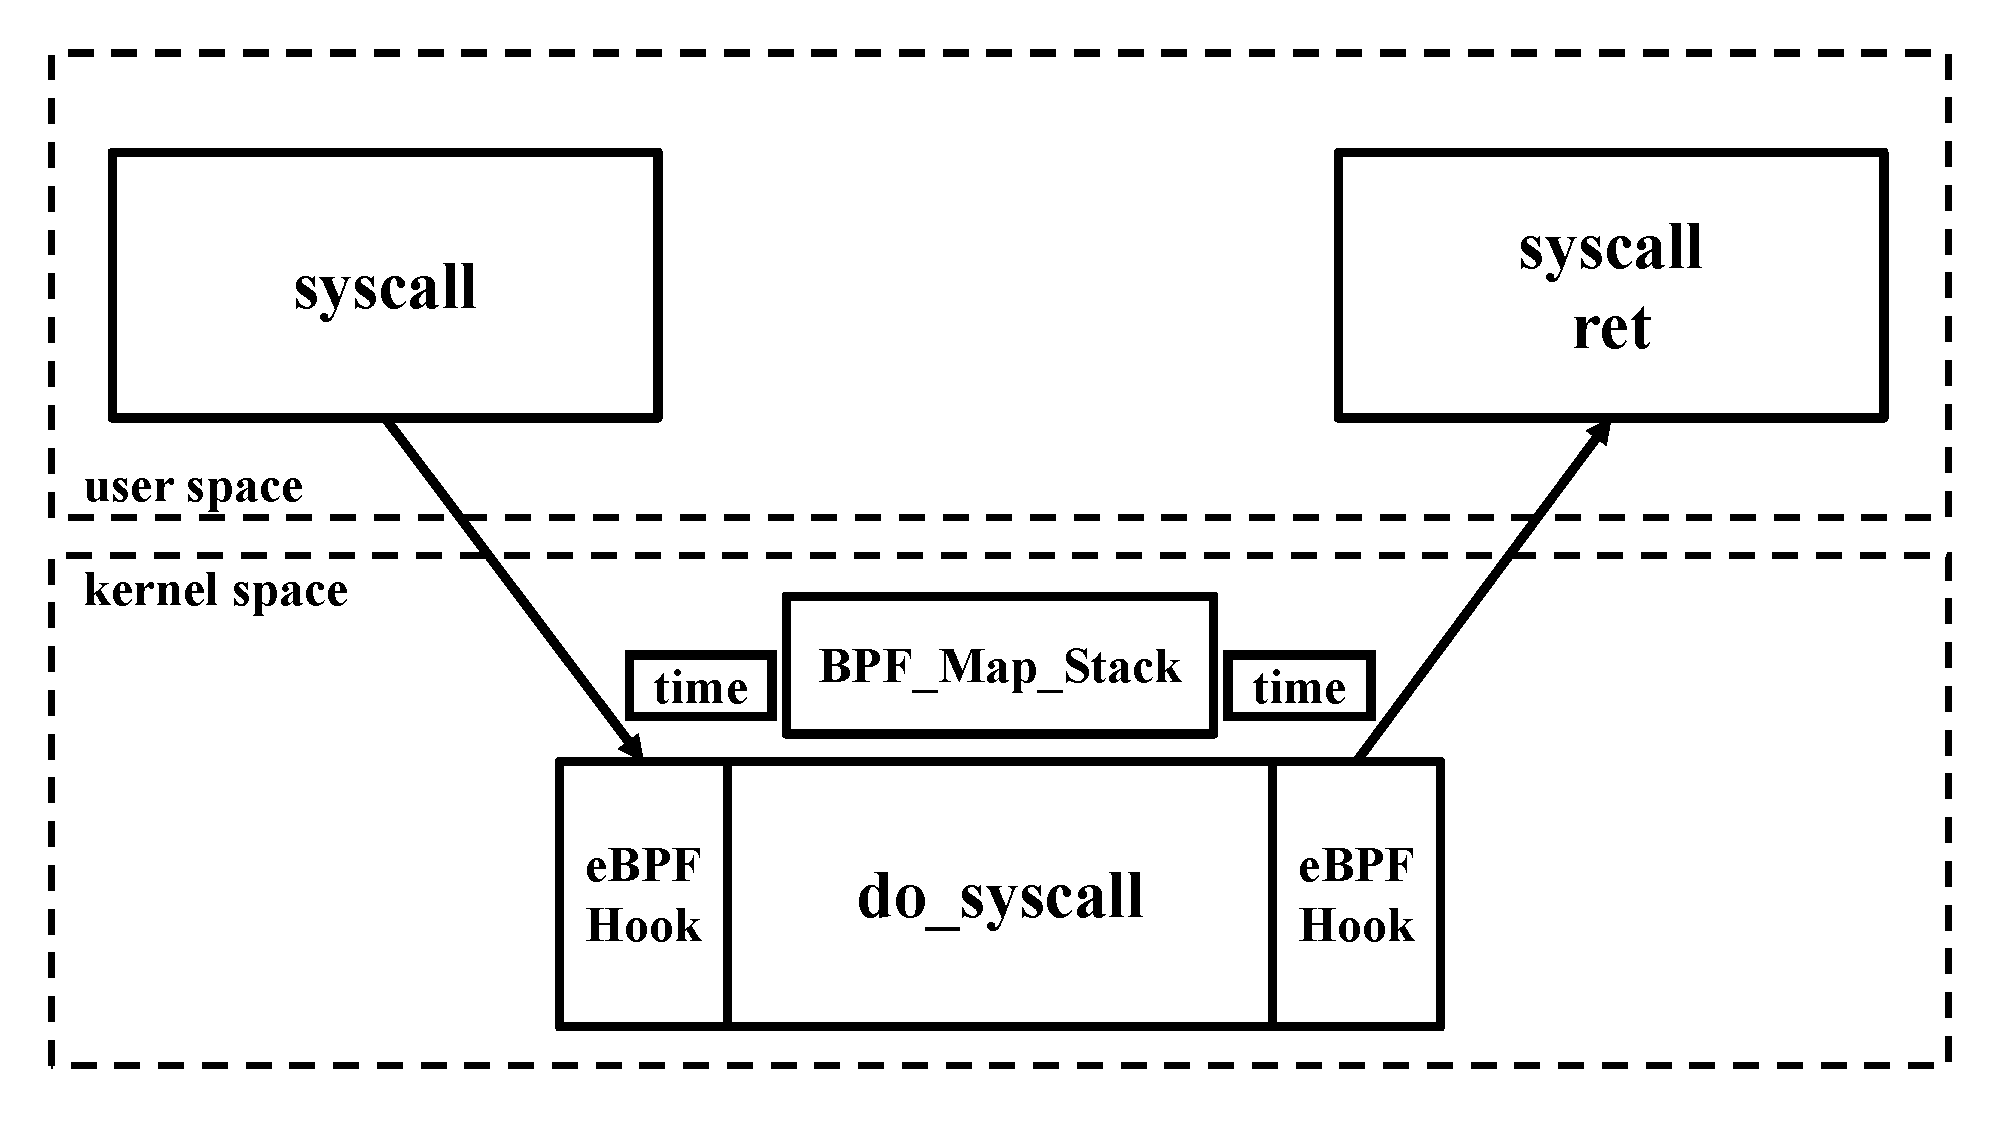
\includegraphics[width=0.7\textwidth]{syscall_hook}
    \bicaption{\quad eBPF Syscall插桩}{\quad eBPF Syscall Hooking}
    \label{fig:syscall_hook}
\end{figure}

5)eBPF Exporter是社区开发的一个监控组件, 提供了内核侧的自定义指标采集。eBPF Exporter能够加载用户编译为字节码的eBPF程序,并通过RingBuffer收集内核侧eBPF程序采集的数据转化为指标。Observed中实现了系统调用及vHost Net内核模块两个eBPF采集程序。内核中系统调用分布在各个子模块中,并通过注册系统调用的方式加入到系统调用表中,用户态应用发起的系统调用会触发一次中断,并最终进入系统调用分发函数,因此可以利用raw tracepoint机制在系统调用分发函数的开始与结束处进行eBPF插桩,如图~\ref{fig:syscall_hook}所示,每当进程进入系统调用中时,首先可以通过BPF Helper函数获取当前task结构体指针,并读取进程号等标识信息,其次通过读取系统调用上下文中的ax寄存器,来获取当前的系统调用号,这两个信息提供了基本的指标标签,基同时,利用BPF Stack来记录时间戳信息,就能够在系统调用返回时计算整个系统调用的执行时间,从而实现对于而对进程每个系统调用吞吐、延迟的监测。vHost Net内核模块的监测则围绕worker内核线程展开,如图~\ref{fig:vhost_net}所示,worker线程中可能执行4种不同的回调函数,分别用于虚拟机的网络发送与接受,通fentry机制过在这些函数的入口与出口出进行插桩,就能够统计出各个函数执行频率以及延时等信息。

\begin{table}[H]
    \bicaption{\quad 指标列表}{\quad Metric list}% caption
    \label{tab:metric_list}
    \footnotesize% fontsize
    \setlength{\tabcolsep}{4pt}% column separation
    \renewcommand{\arraystretch}{1.5}% ro w space 
    \centering
    \begin{tabular}{lcc}
        \hline
        %\multicolumn{num_of_cols_to_merge}{alignment}{contents} \\
        %\cline{i-j}% partial hline from column i to column j
        层级 & 来源 & 指标\\
        \hline
        Host & Kernel(271) & [cpu] sys\_time、user\_time、freq ... \\
        & & [mem] usage、avail、swapfree、bounce、hugepage ...\\
        & & [network] transmit、netstat、sockstat、ip、speed ...\\
        & & [disk]flush requests、flush request time、read、write ...\\
        & & ...\\
        & eBPF(2) & [syscall] count、duration\\
        & Resctrl(3) & llc cap、mem b/w local、mem b/w total\\
        Hypervisor & Libvirt(68) & [vcpu] sys\_time、user\_time、wait、delay...\\
        & & [mem] usable、avail、dick cache、rss ...\\
        & & [perf] cycle、instruction、cache miss ...\\
        & & [block] flush request、flush time、read、write ...\\
        & & [interface] receive、transmit ...\\
        & & ...\\
        & KVM(59) & vm\_exit、io\_exit、irq\_exit、irq\_inject、halt\_poll ...\\
        App & Log/Envoy & qos, latency, rate, score ...\\
        \hline
    \end{tabular}
\end{table}

\section{实验设计}

\subsection{基准性能实验}

实验中使用两台C6服务器作为Client和Server,服务器具体配置如表~\ref{tab:c6_info}所示,其中Client服务器额外承担实验管理的功能,同时作为Observer角色部署Prometheus Server等组件,而Server主要承载具体的应用,同时作为Observed角色部署上述设计实现的6种Exporter,并为Exporter设置Numa亲和性以避免对应用产生干扰。基准性能实验测试无干扰情况下各个应用的基础性能,对于每个典型应用,使用华为云提供的竖亥Benchmark中的模拟负载多样的负载来监测不同场景下的基准性能。

\begin{table}[H]
    \bicaption{\quad C6服务器信息}{\quad C6 Information}% caption
    \label{tab:c6_info}
    \footnotesize% fontsize
    \setlength{\tabcolsep}{4pt}% column separation
    \renewcommand{\arraystretch}{1.5}% row space 
    \centering
    \begin{tabular}{lc}
        \hline
        类型 & 信息 \\
        \hline
        OS & Ubuntu 22.04 ( Kernel 5.15.0) \\
        CPU & Intel Xeon Gold 6151 (18 cores) * 2 \\
        Processor Core Frequency & 3GHz,Turbo 3.4GHz \\
        L1 Caches & 32KB *,  8-way set associative, split D/I \\
        L2 Caches & 1024KB, 16-way set associative \\
        L3 Caches & 25344KB, 11-way set associative \\
        Main Memory & 32GB * 12, 2666MHz DDR4 \\
        Storage & Avago MegaRAID, 2.18T SAS RAID0, 87.322T SATA RAID0 \\
        NIC & Intel Corporation Ethernet Connection X722 for 10GbE SFP+(10Gbit) \\
        \hline
    \end{tabular}
\end{table}

% 1)Redis、Memcached。使用memtier_benchmark来产生负载,负载的模型由华为云提供,包括Normal、Random两类模拟负载

% 2)Mysql。使用TPCC作为基准实验负载

% 3)Elasticsearch。使用YCSB作为基准负载

% 4)Kafka。

% 5)Nginx。

% 6)Render。使用华为内部的模拟负载。

\subsection{性能劣化实验}

% 干扰应用
% - 干扰有效性
% - 噪声控制

性能劣化实验通过增加目标应用与干扰应用的混部场景,分析应用对于不同干扰类型的敏感程度。在干扰应用的选择上,使用stress-ng来产生不同类型的干扰。stress-ng是Linux系统中常用的压力测试工具,能够模拟各种资源的压力场景,而实验中则利用其模拟各种压力场景的特性来制造干扰,并观测目标应用的性能劣化情况。stress-ng提供了丰富的配置参数,本课题选用如表~\ref{tab:arg_list}所示的参数配置,来制造CPU、Cache、内存、IO、Network上的干扰。

\begin{table}[H]
    \bicaption{\quad stress\_ng 实验参数列表}{\quad stress\_ng args list}% caption
    \label{tab:arg_list}
    \footnotesize% fontsize
    \setlength{\tabcolsep}{4pt}% column separation
    \renewcommand{\arraystretch}{1.5}% row space 
    \centering
    \begin{tabular}{lcc}
        \hline
        %\multicolumn{num_of_cols_to_merge}{alignment}{contents} \\
        %\cline{i-j}% partial hline from column i to column j
        子系统 & 参数 & 说明\\
        \hline
        CPU	    & --cpu & 循环执行sqrt(rand())的线程数量\\
	            & --cpu-load & 线程负载的比率\\
        Cache	& --cache & cache抖动线程数量\\
	            & --cache-level	&测试指定等级的Cache\\
	            & --icache	&指令cache抖动的线程数量\\
        IO	    & --io	&循环执行sync()的线程数量\\
	            & --iomix	&执行混合I/O操作的线程数量\\
	            & --hdd	&循环执行write()/unlink()的线程数量\\
	            & --seek	&执行随机seek I/O的线程数量\\
        Memory	& --vm	&循环执行匿名mmap的线程数量\\
	            & --vm-bytes	&执行vm操作的buffer大小\\
	            & --memrate	&执行read/writes的线程数量\\
	            & --memrate-bytes	&执行内存操作的buffer大小\\
	            & --malloc	&执行malloc/realloc/free的线程数量\\
	            & --memcpy	&执行memory copy的线程数量\\
        Network	& --sock	&执行Socket I/O的线程数量\\
	            & --epoll	&执行epoll处理的线程数量\\
        \hline
    \end{tabular}
\end{table}

正式干扰实验之前,首先需要验证干扰的效果。测试实验使用一个4 CPU 8G Memory虚拟机,并在其中按照上述配置运行stress-ng干扰应用。干扰强度的定义与配置的stress-ng线程相关,对于CPU干扰,采用线性的干扰强度,即干扰强度正比于CPU负载,而对于其他干扰则使用指数映射,即干扰强度与线程数量呈指数关系,以便于快速探测干扰峰值。具体实验的结果从可观测性系统中获取,每种干扰选择一个表征指标用以说明,具体结果如图~\ref{fig:interference}所示。

1)CPU干扰选择CPU Usage作为表征指标,干扰效果如~\ref{fig:cpu_interference}所示,可见随干扰强度的不断提升,干扰应用逐渐能够占用所有的核心资源。

2)Cache干扰选择Cache Usage作为表征指标,干扰效果如图~\ref{fig:cache_interference}所示,可见随干扰强度的不断上升,干扰应用逐渐能够占用全部的LLC。同时,当干扰强度上升至5之后,Cache Usage就几乎稳定在峰值。

3)IO干扰选择IO Input Bytes作为表征指标,干扰效果如图~\ref{fig:io_interference}所示,在前段,随干扰强度的上升,干扰应用占用越来越多的IO带宽,但当干扰强度超过5之后,干扰应用占用的IO带宽反而开始减少。由于IO干扰强度与干扰线程数量指数相关,高干扰强度下会产生大量的IO线程,这些线程彼此之间会相互竞争,因此导致整体的IO带宽下降。

\begin{figure}[H]
  \centering
  \begin{subfigure}[b]{0.45\textwidth}
    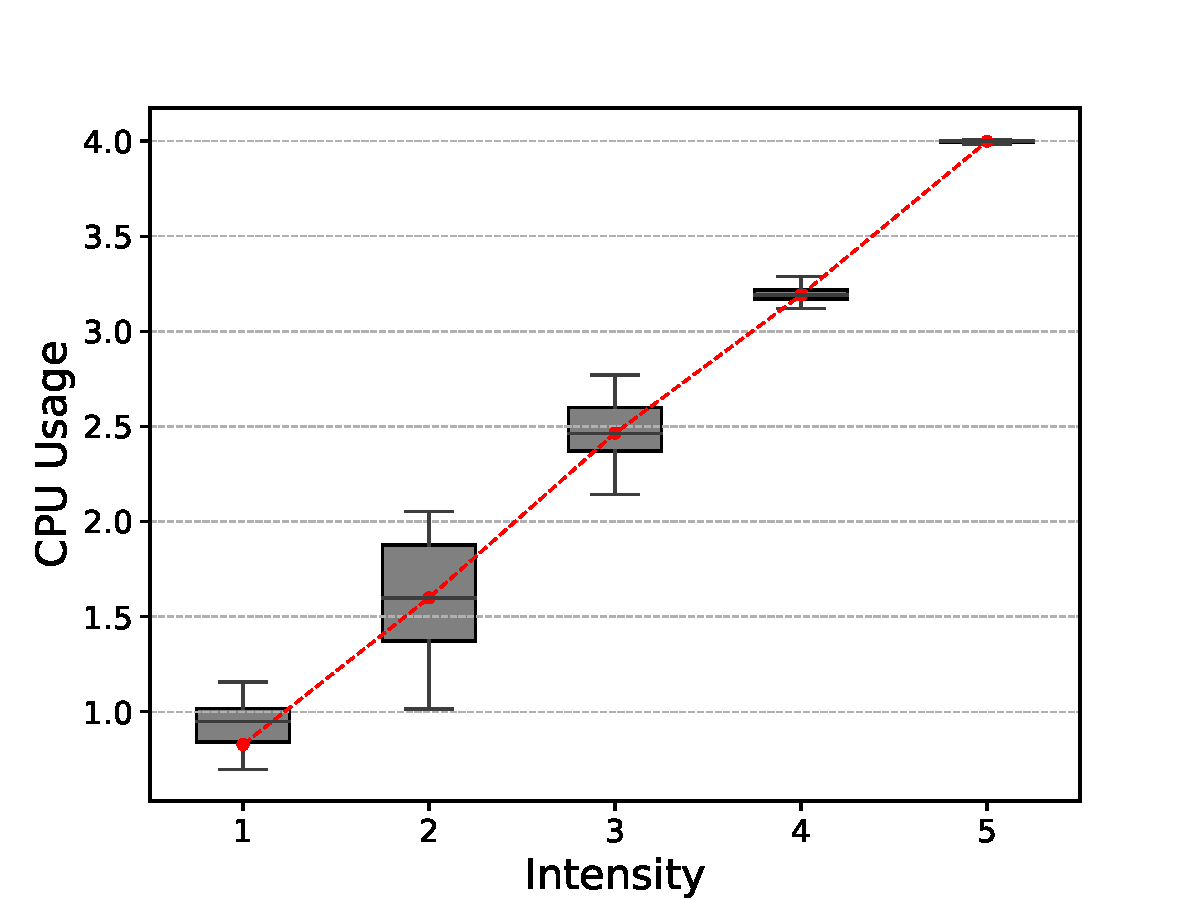
\includegraphics[width=\textwidth]{cpu_interference}
    \caption{cpu干扰效果}
    \label{fig:cpu_interference}
  \end{subfigure}
  \begin{subfigure}[b]{0.45\textwidth}
    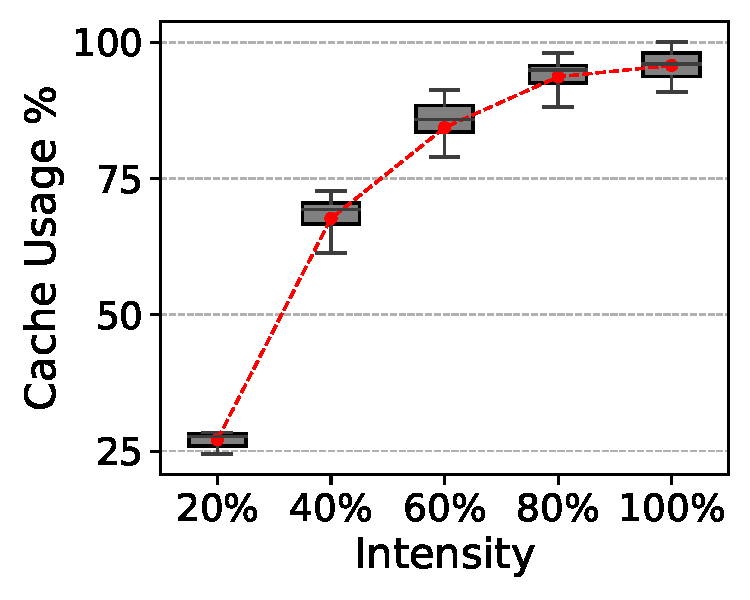
\includegraphics[width=\textwidth]{cache_interference}
    \caption{cache干扰效果}
    \label{fig:cache_interference}
  \end{subfigure}
  \begin{subfigure}[b]{0.45\textwidth}
    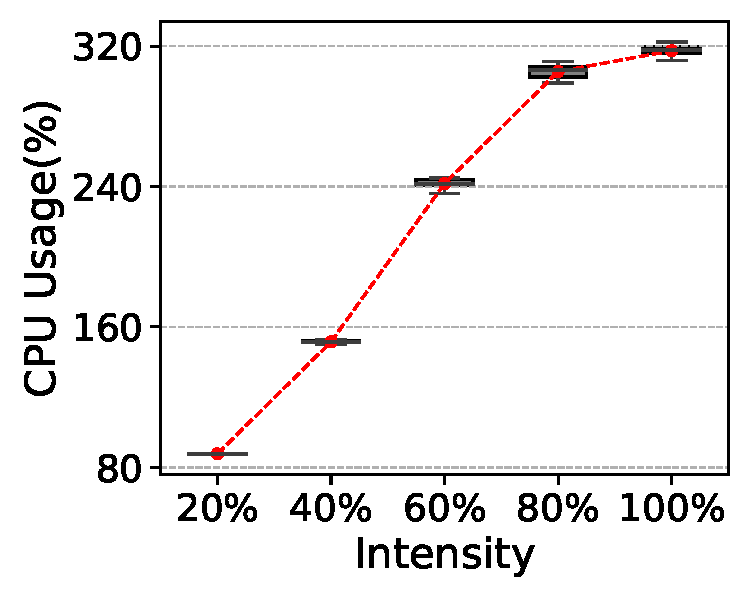
\includegraphics[width=\textwidth]{io_interference}
    \caption{io干扰效果}
    \label{fig:io_interference}
  \end{subfigure}
  \begin{subfigure}[b]{0.45\textwidth}
    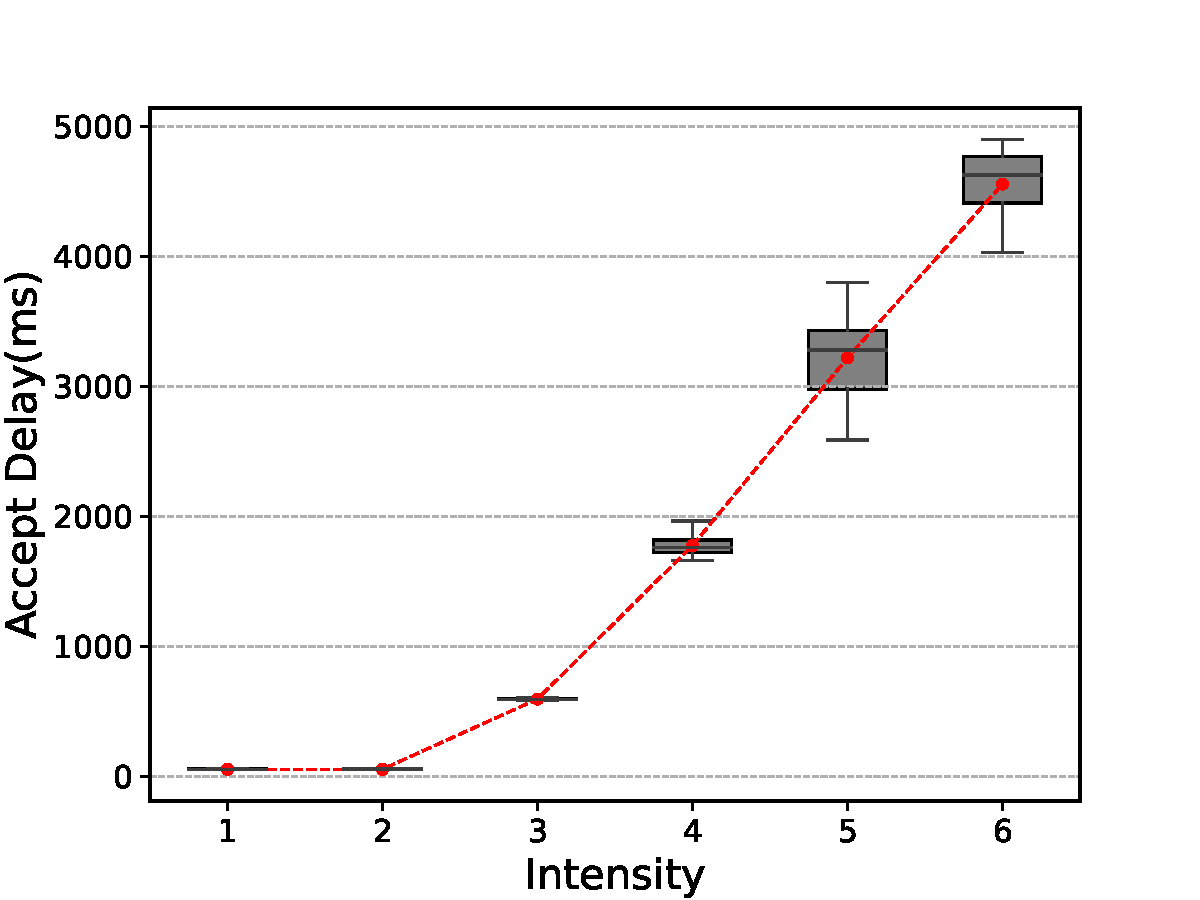
\includegraphics[width=\textwidth]{net_interference}
    \caption{net干扰效果}
    \label{fig:net_interference}
  \end{subfigure}
  \begin{subfigure}[b]{0.45\textwidth}
    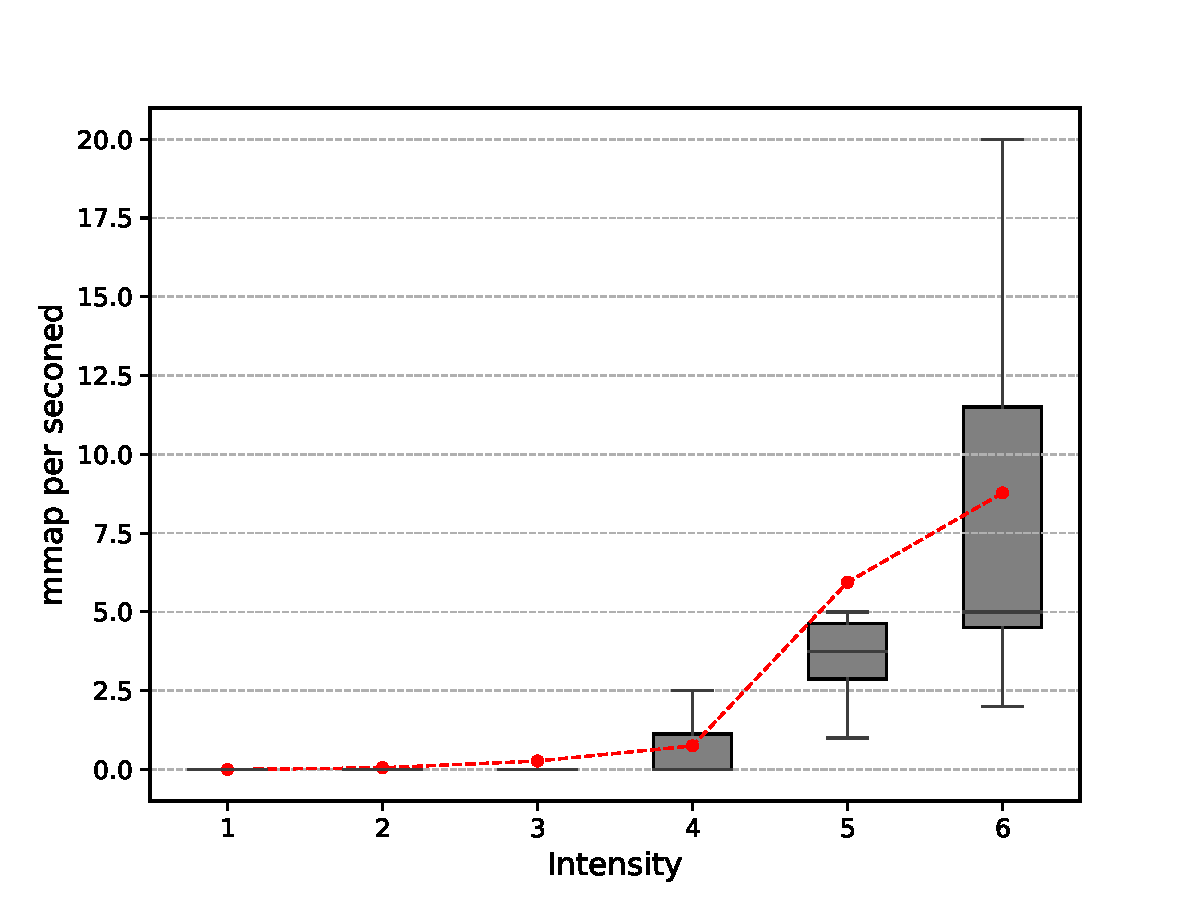
\includegraphics[width=\textwidth]{vm_interference}
    \caption{内存干扰效果}
    \label{fig:vm_interference}
  \end{subfigure}
  \bicaption{\quad 干扰效果分析}{\quad Interference Effects Analysis}
  \label{fig:interference}
\end{figure}

4)Net干扰选择Accept系统调用延迟作为表征指标。Accept系统调用通常发生在Server类应用中,用于与Client建立连接,Accept系统调用变慢通常意味着连接排队延迟与客户端超时,而具体的干扰效果如图~\ref{fig:net_interference}所示,可见随干扰强度的不断上升,Accept系统调用的延迟逐渐变大,由于延迟指标可以无限增加,实验中根据应用延迟范围来确定干扰强度。

5)Memory干扰使用每秒的mmap系统调用次数作为表征指标。stress-ng通过频繁地调用mmap来产生内存干扰,如图~\ref{fig:vm_interference}所示,随干扰强度的上升,每秒的mmap系统调用数量也在不断上升,并在干扰强度为6时出现较大的波动。

考虑到干扰效果评测结果中,Net干扰实际上使用的是本地回环网络,因此并不能实质性地在网络流量上产生干扰,导致类似于CPU或Cache干扰,因此在后续的
没有采用Net干扰项作为测试项,而是根据典型应用的类型,如是否是网络应用来判断应用的网络敏感性。

\section{画像分析与结论}

\subsection{典型应用资源使用倾向分析}

无干扰实验中计算各个监测指标的变异系数,得到不同应用对应的资源指标如图~\ref{fig:resource_affinity}所示。

\begin{figure}[H]
    \centering
    \begin{subfigure}[b]{0.49\textwidth}
      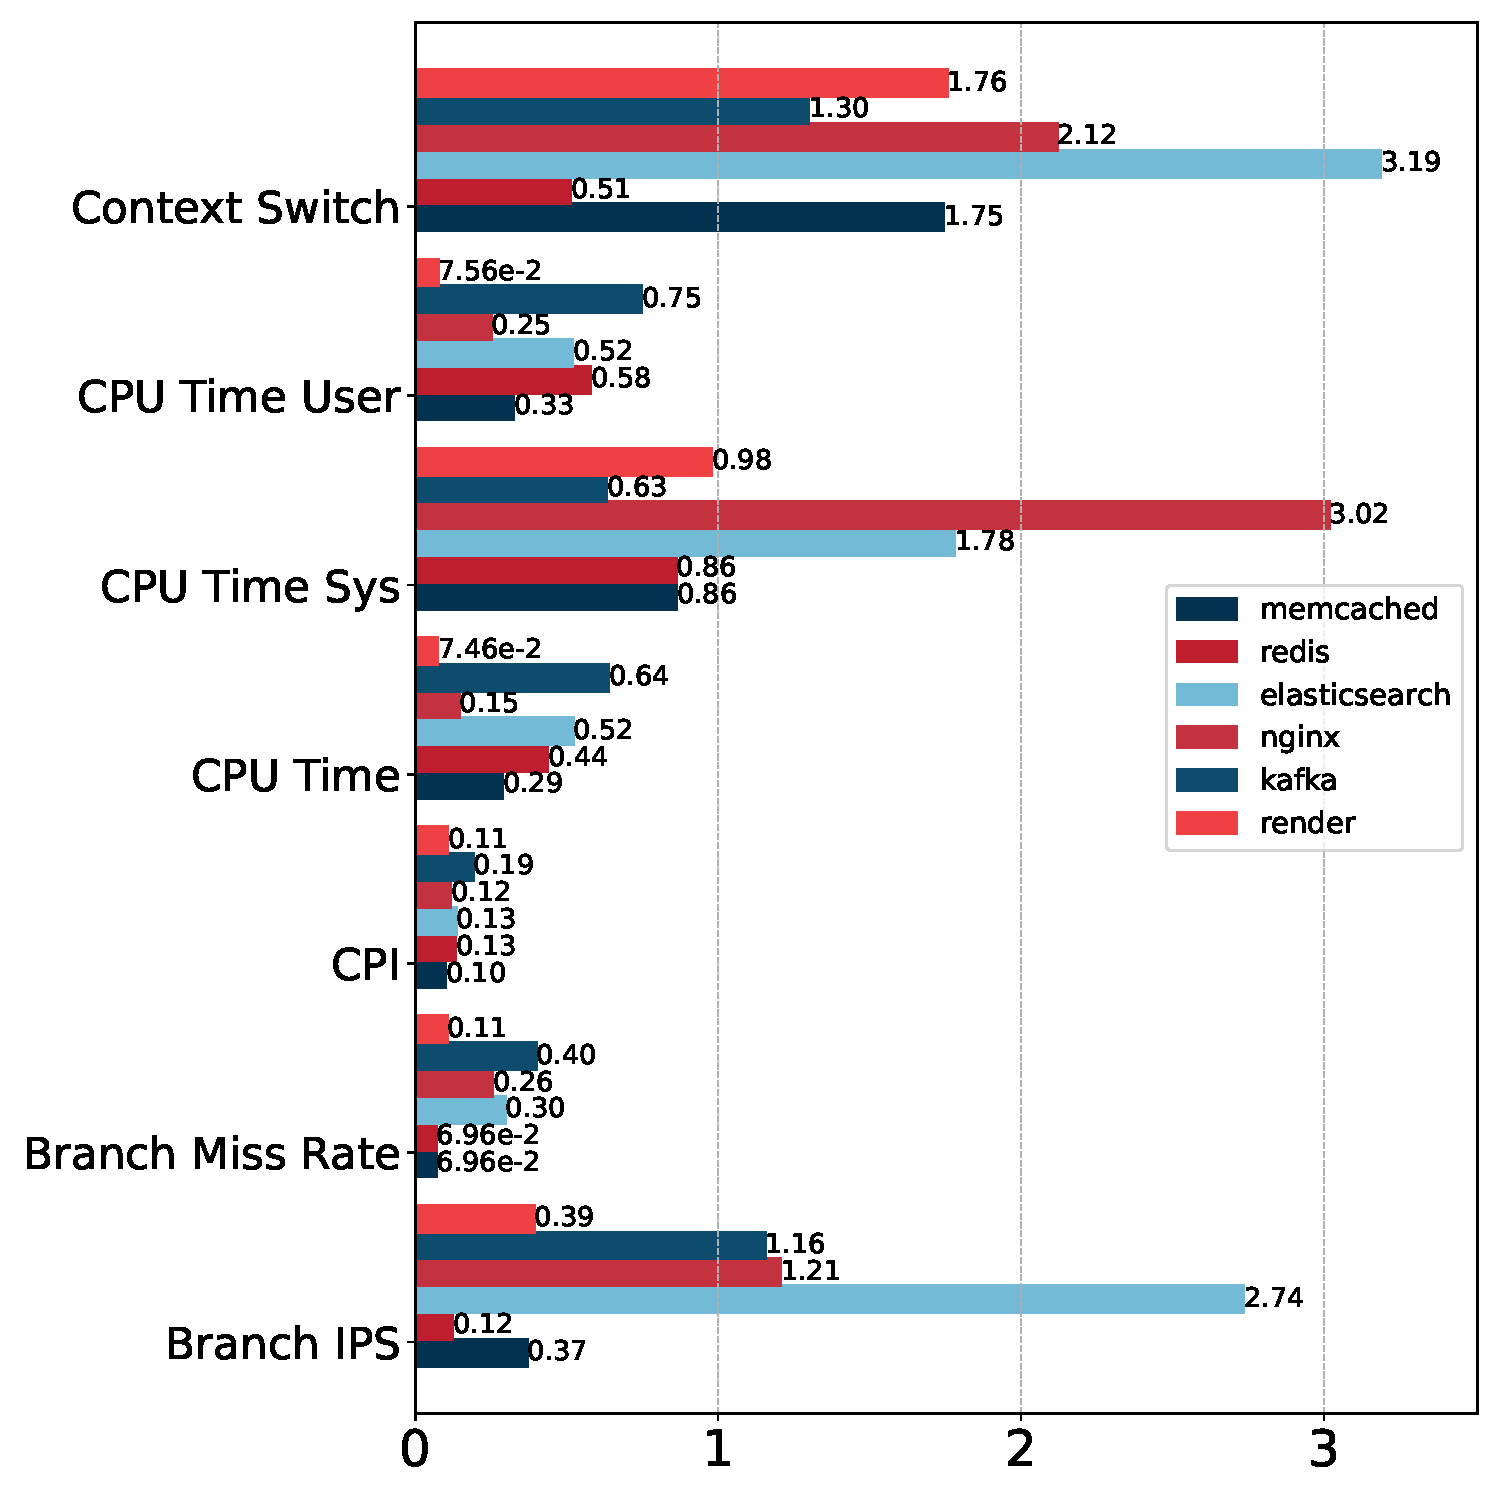
\includegraphics[width=\textwidth]{cof_cpu}
      \caption{CPU资源指标}
      \label{fig:cof_cpu}
    \end{subfigure}
    \begin{subfigure}[b]{0.49\textwidth}
        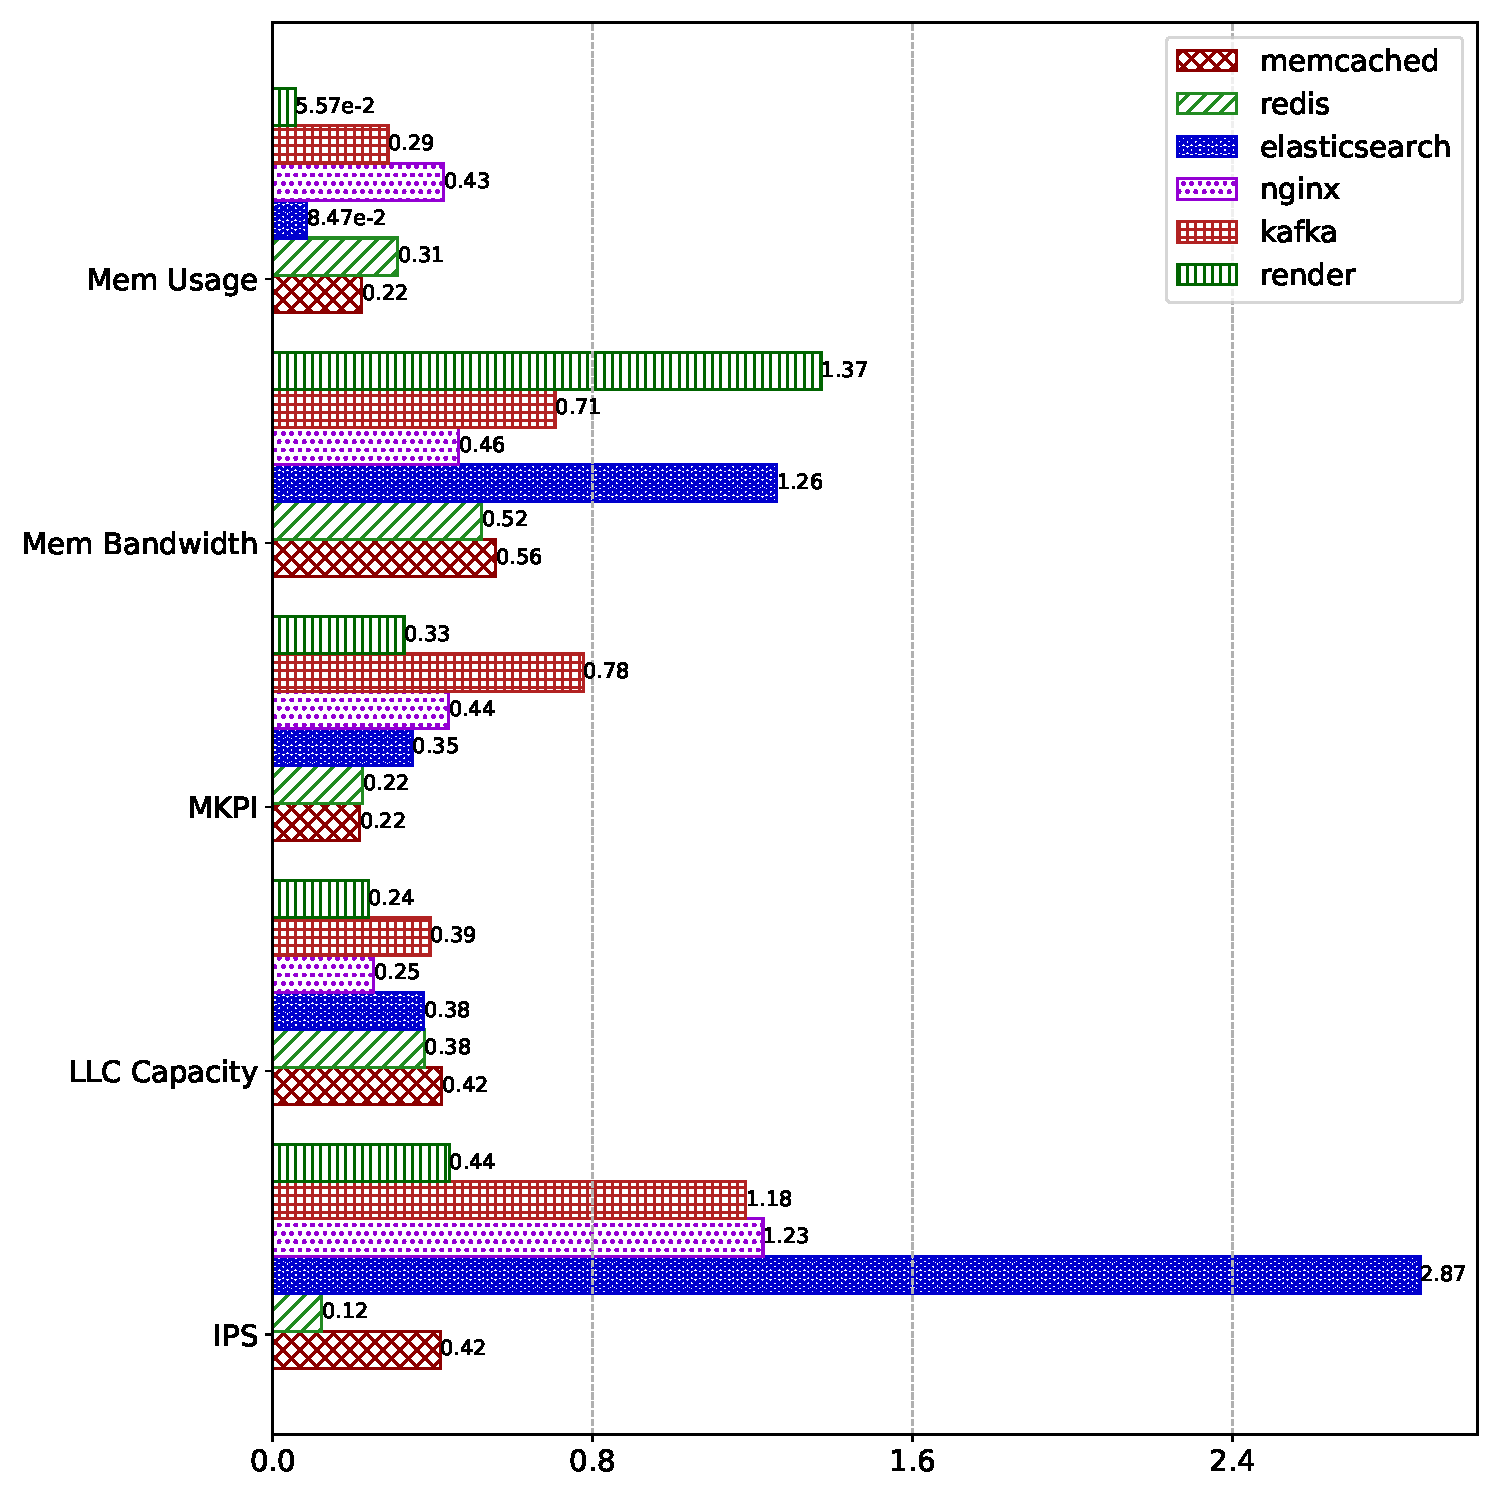
\includegraphics[width=\textwidth]{cof_mem}
        \caption{Cache、内存资源指标}
        \label{fig:cof_mem}
    \end{subfigure}
    \begin{subfigure}[b]{0.49\textwidth}
        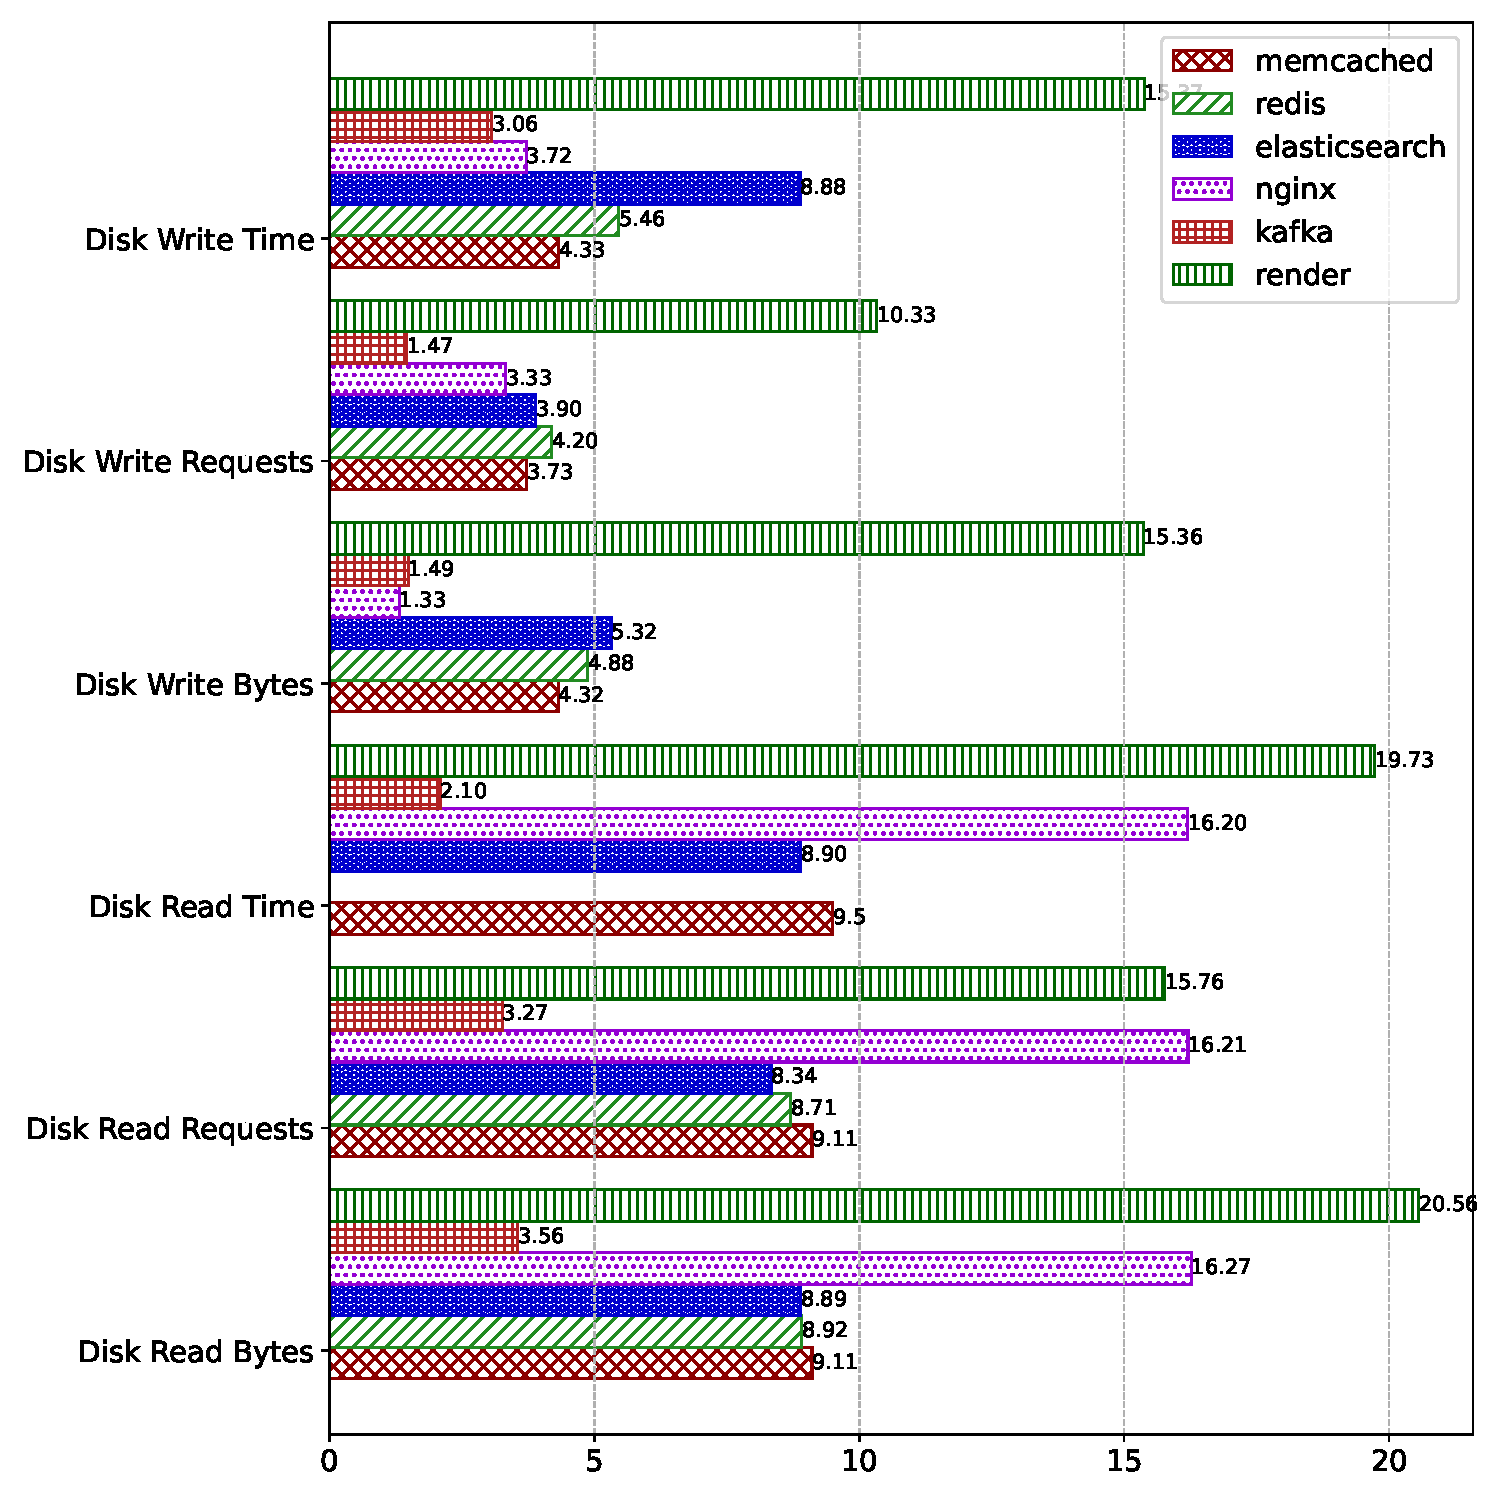
\includegraphics[width=\textwidth]{cof_io}
        \caption{IO资源指标}
        \label{fig:cof_mem}
    \end{subfigure}
    \begin{subfigure}[b]{0.49\textwidth}
        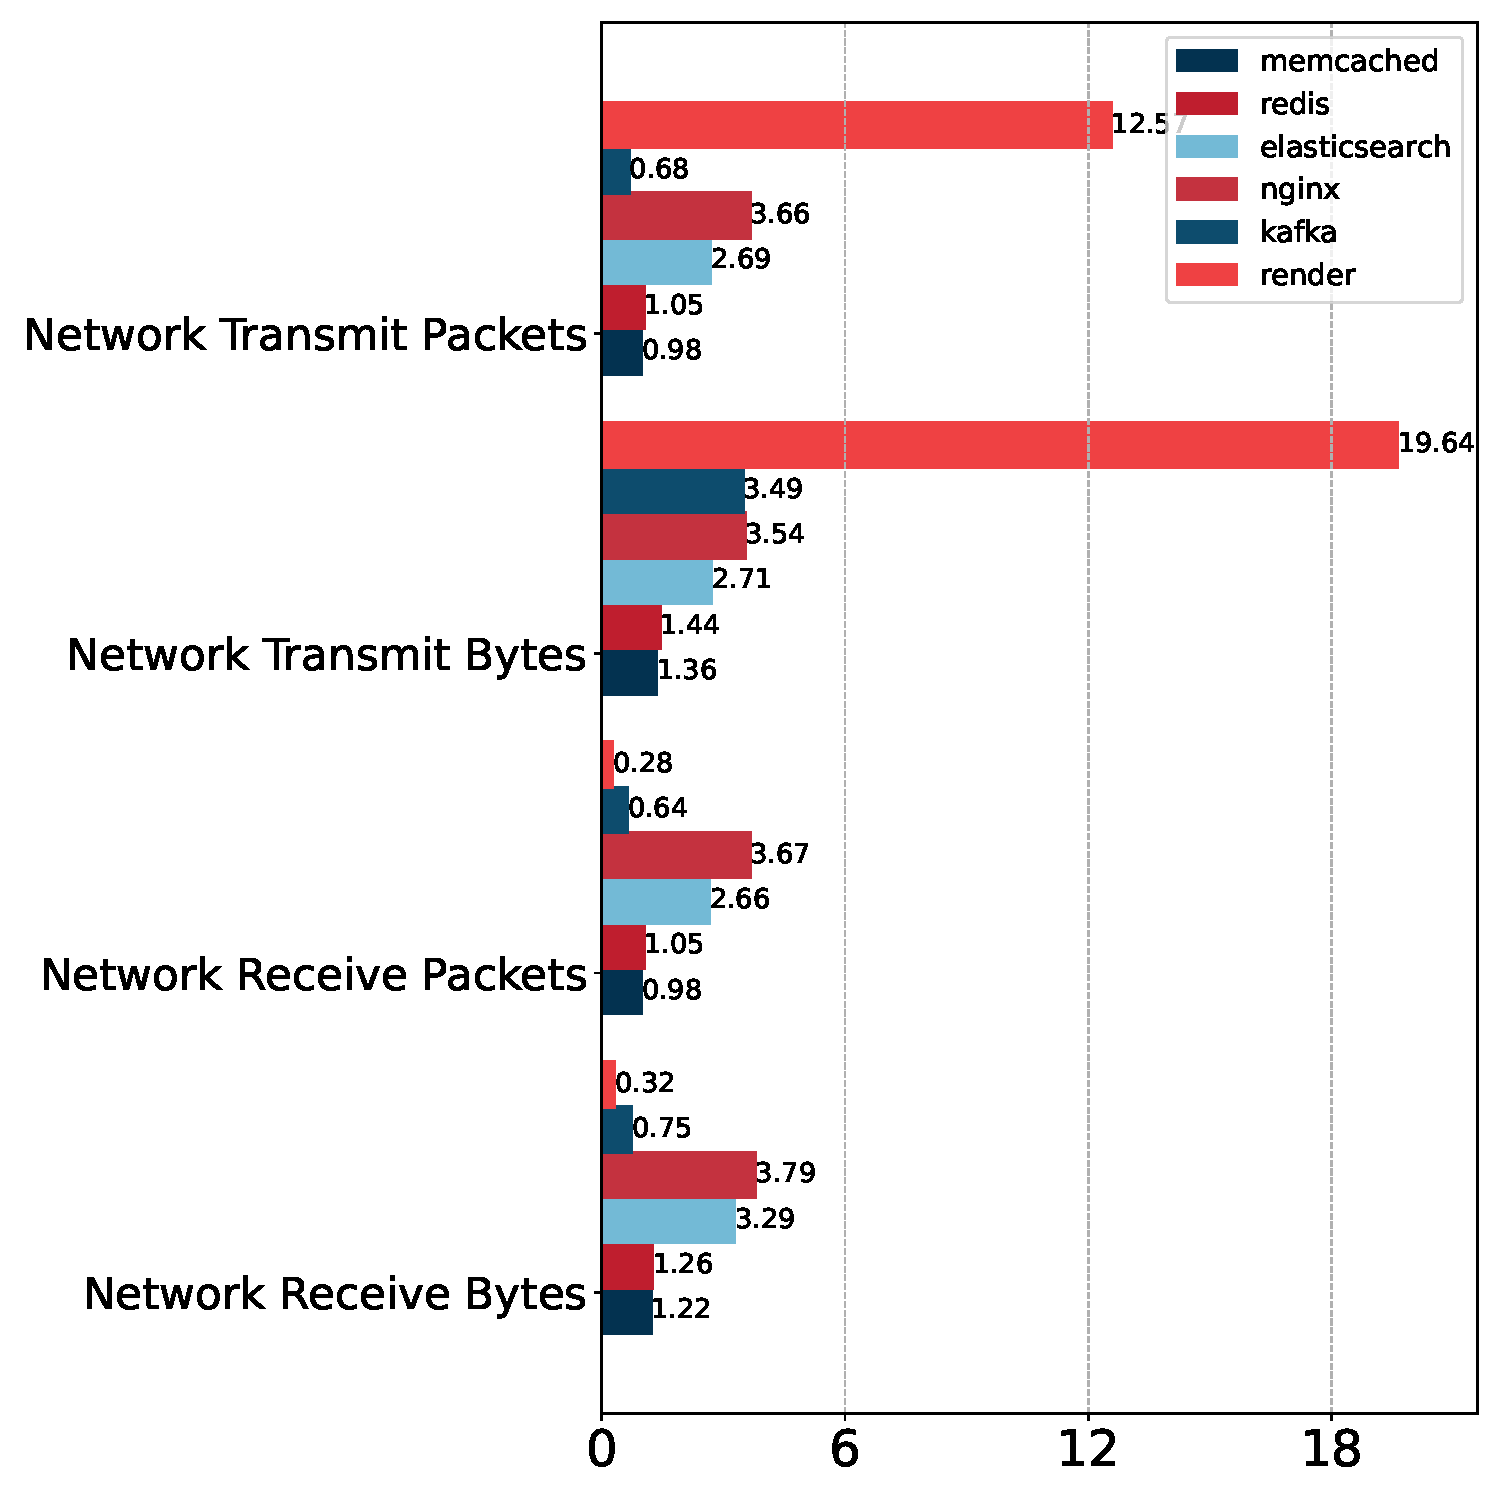
\includegraphics[width=\textwidth]{cof_network}
        \caption{网络资源指标}
        \label{fig:cof_mem}
    \end{subfigure}
\bicaption{\quad 总资源变异系数}{\quad Coefficient of Variation of Total Resources}
\label{fig:resource_affinity}
\end{figure}

从整体上看,Block I/O与Network I/O两类指标在不同应用之间呈现出较大的差异,相同指标在不同应用中的极大值与极小值差异可达$10^4$--$10^5$倍,而其余指标的差异通常不会超过20倍,这就导致图中一部分应用I/O相关指标非常高,而另一部分应用的相同指标则始终为一个较低的值。而在其他指标上则没有体现明显的差异度,这有如下两方面原因,首先,对于"利用率"类型的指标,这些指标存在明确的上下界,同时数值上的差异度难以直接体现,如对于CPU利用率,80\%与90\%利用率仅有约12\%的数值差异,但计算空闲CPU占比,则前者是后者的200\%,对于这些指标不能简单地使用差异度度量。其次,一些与硬件相关的指标波动不明显,如CPI,其波动通常受到流水线周期、指令阻塞和回退的数量等因素影响,在优化较好的现代处理器平台上,通常只会在一个较小的范围内波动。

\begin{figure}[H]
    \centering
    \begin{subfigure}[b]{0.9\textwidth}
      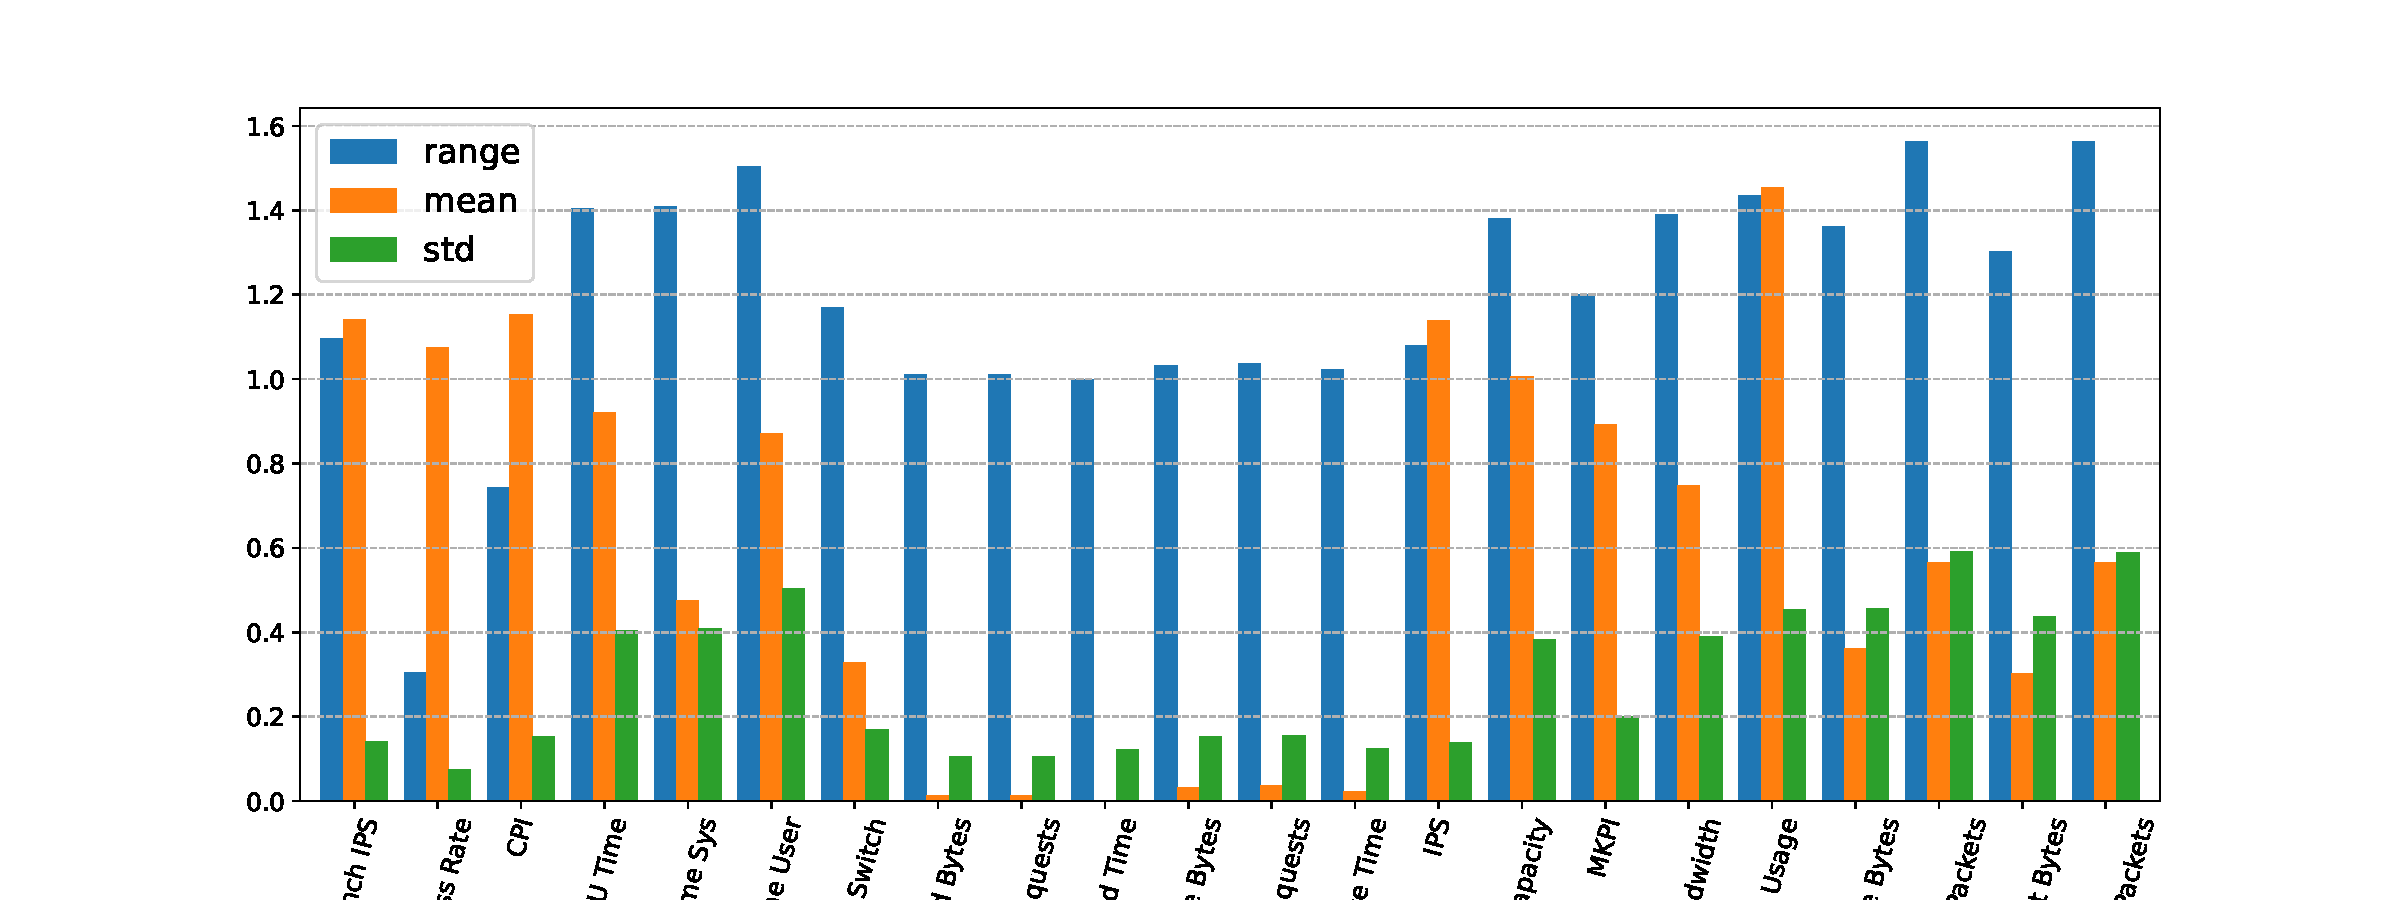
\includegraphics[width=\textwidth]{profile_redis}
      \caption{Redis资源使用}
      \label{fig:profile_redis}
    \end{subfigure}
    \begin{subfigure}[b]{0.9\textwidth}
        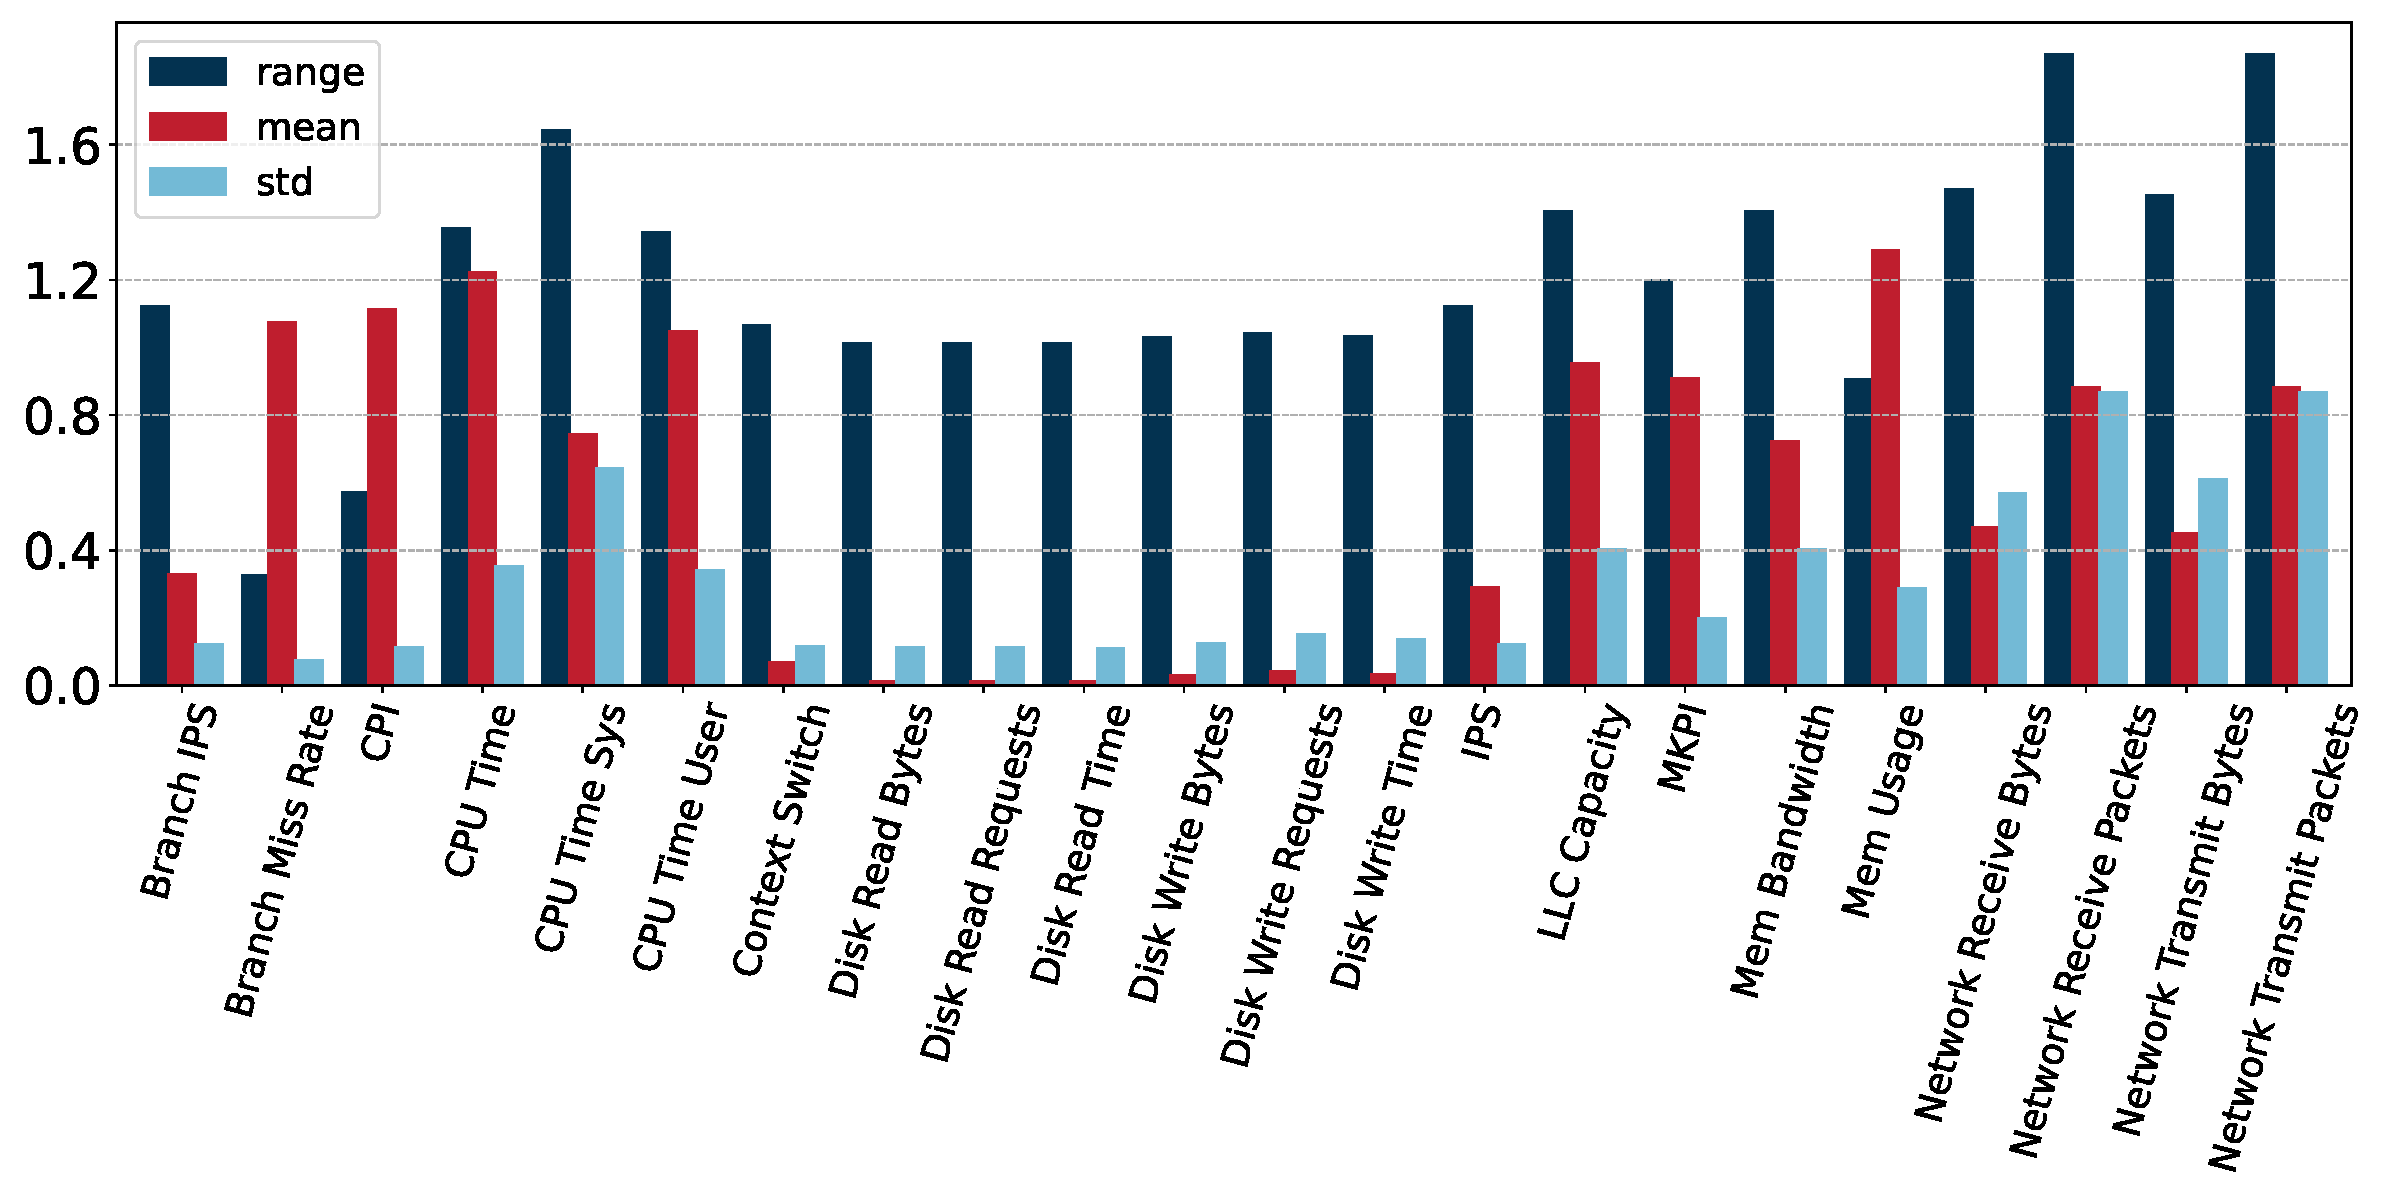
\includegraphics[width=\textwidth]{profile_memcached}
        \caption{Memcached资源使用}
        \label{fig:profile_memcached}
    \end{subfigure}
\bicaption{\quad Redis与Memcached资源使用情况}{\quad Resource Usage of Redis and Memcached}
\label{fig:resource_affinity_0}
\end{figure}

具体到应用的差异性如图~\ref{fig:resource_affinity_0}所示,不同应用对于主要的5种系统资源的需求呈现处较大的差异:

1)CPU资源:应用的运行都需要CPU资源, 而不同应用对于CPU资源的使用上存在差异。Kafka运行时需要较多的CPU资源,体现在较高的IPS指标上。Redis、Memcached同样对于CPU资源有较高需求,从较多的平均CPU时间片占用能够看出,但不同之处在于,Redis、Memcached对于CPU资源的使用与请求强相关,在请求量较低时,由于频繁的睡眠与唤醒,此时不仅CPU资源需求少,同时CPI也较高,而当请求量足够多时,由于都基于epoll实现,因此密集的请求使得两者总是能够保持CPU的占用,而相较于Redis,Memcached在默认配置下更能够利用多核优势。Render应用同样需要较多的CPU资源,但与上述应用不同的是,Render在CPU资源使用上相当稳定,这一特点反映在较低的Branch IPS及Context Switch指标上。

\begin{figure}[H]
    \centering
    \begin{subfigure}[b]{0.9\textwidth}
      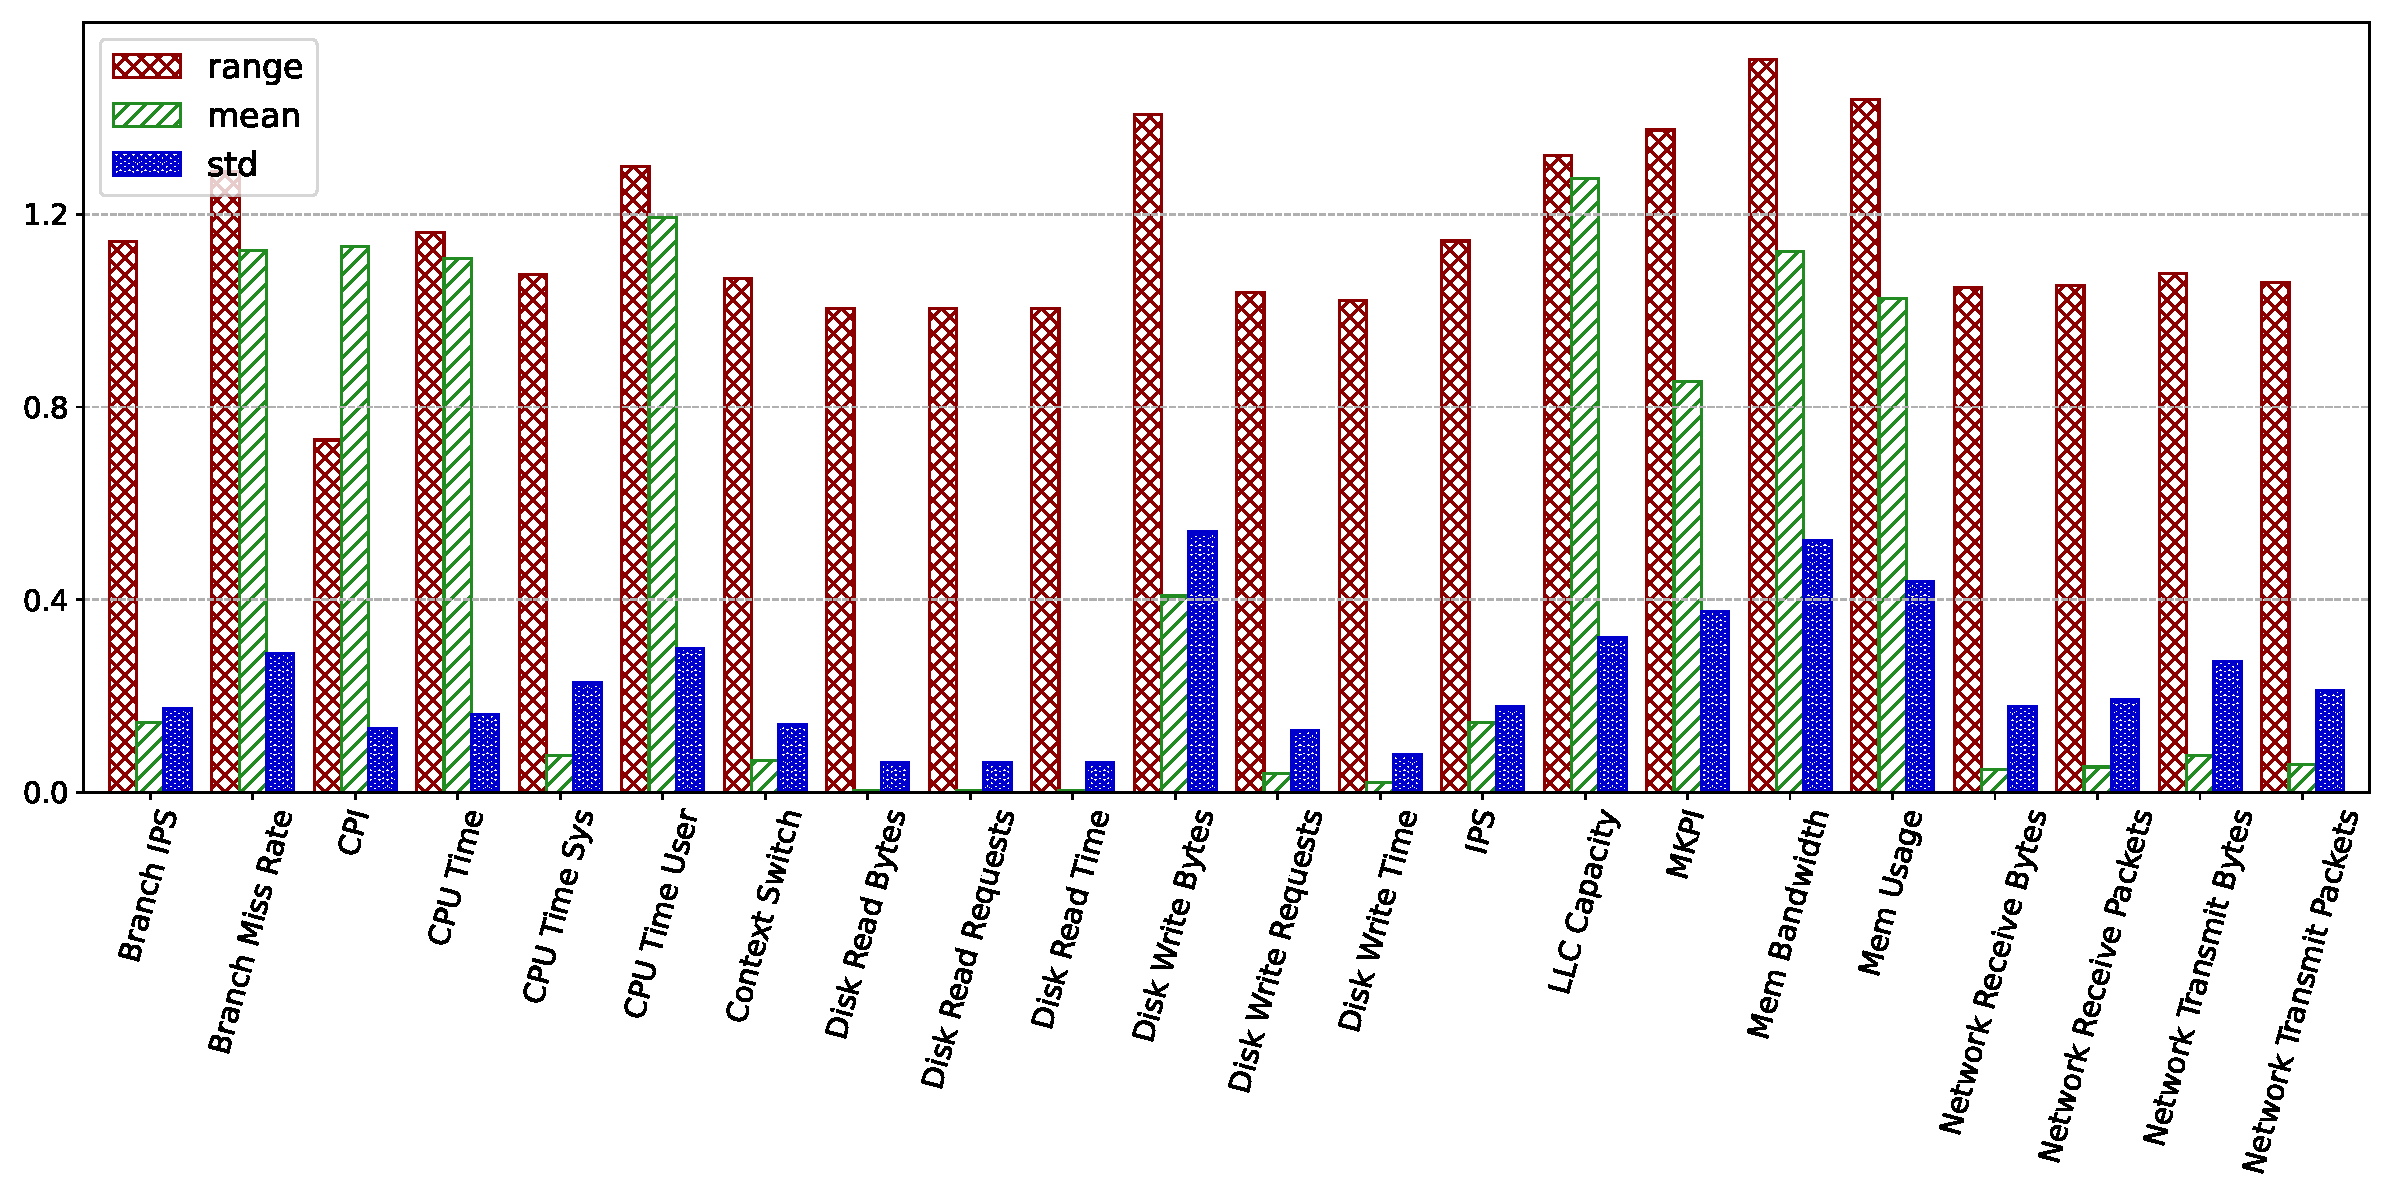
\includegraphics[width=\textwidth]{profile_nginx}
      \caption{Nginx资源使用}
      \label{fig:profile_nginx}
    \end{subfigure}
    \begin{subfigure}[b]{0.9\textwidth}
        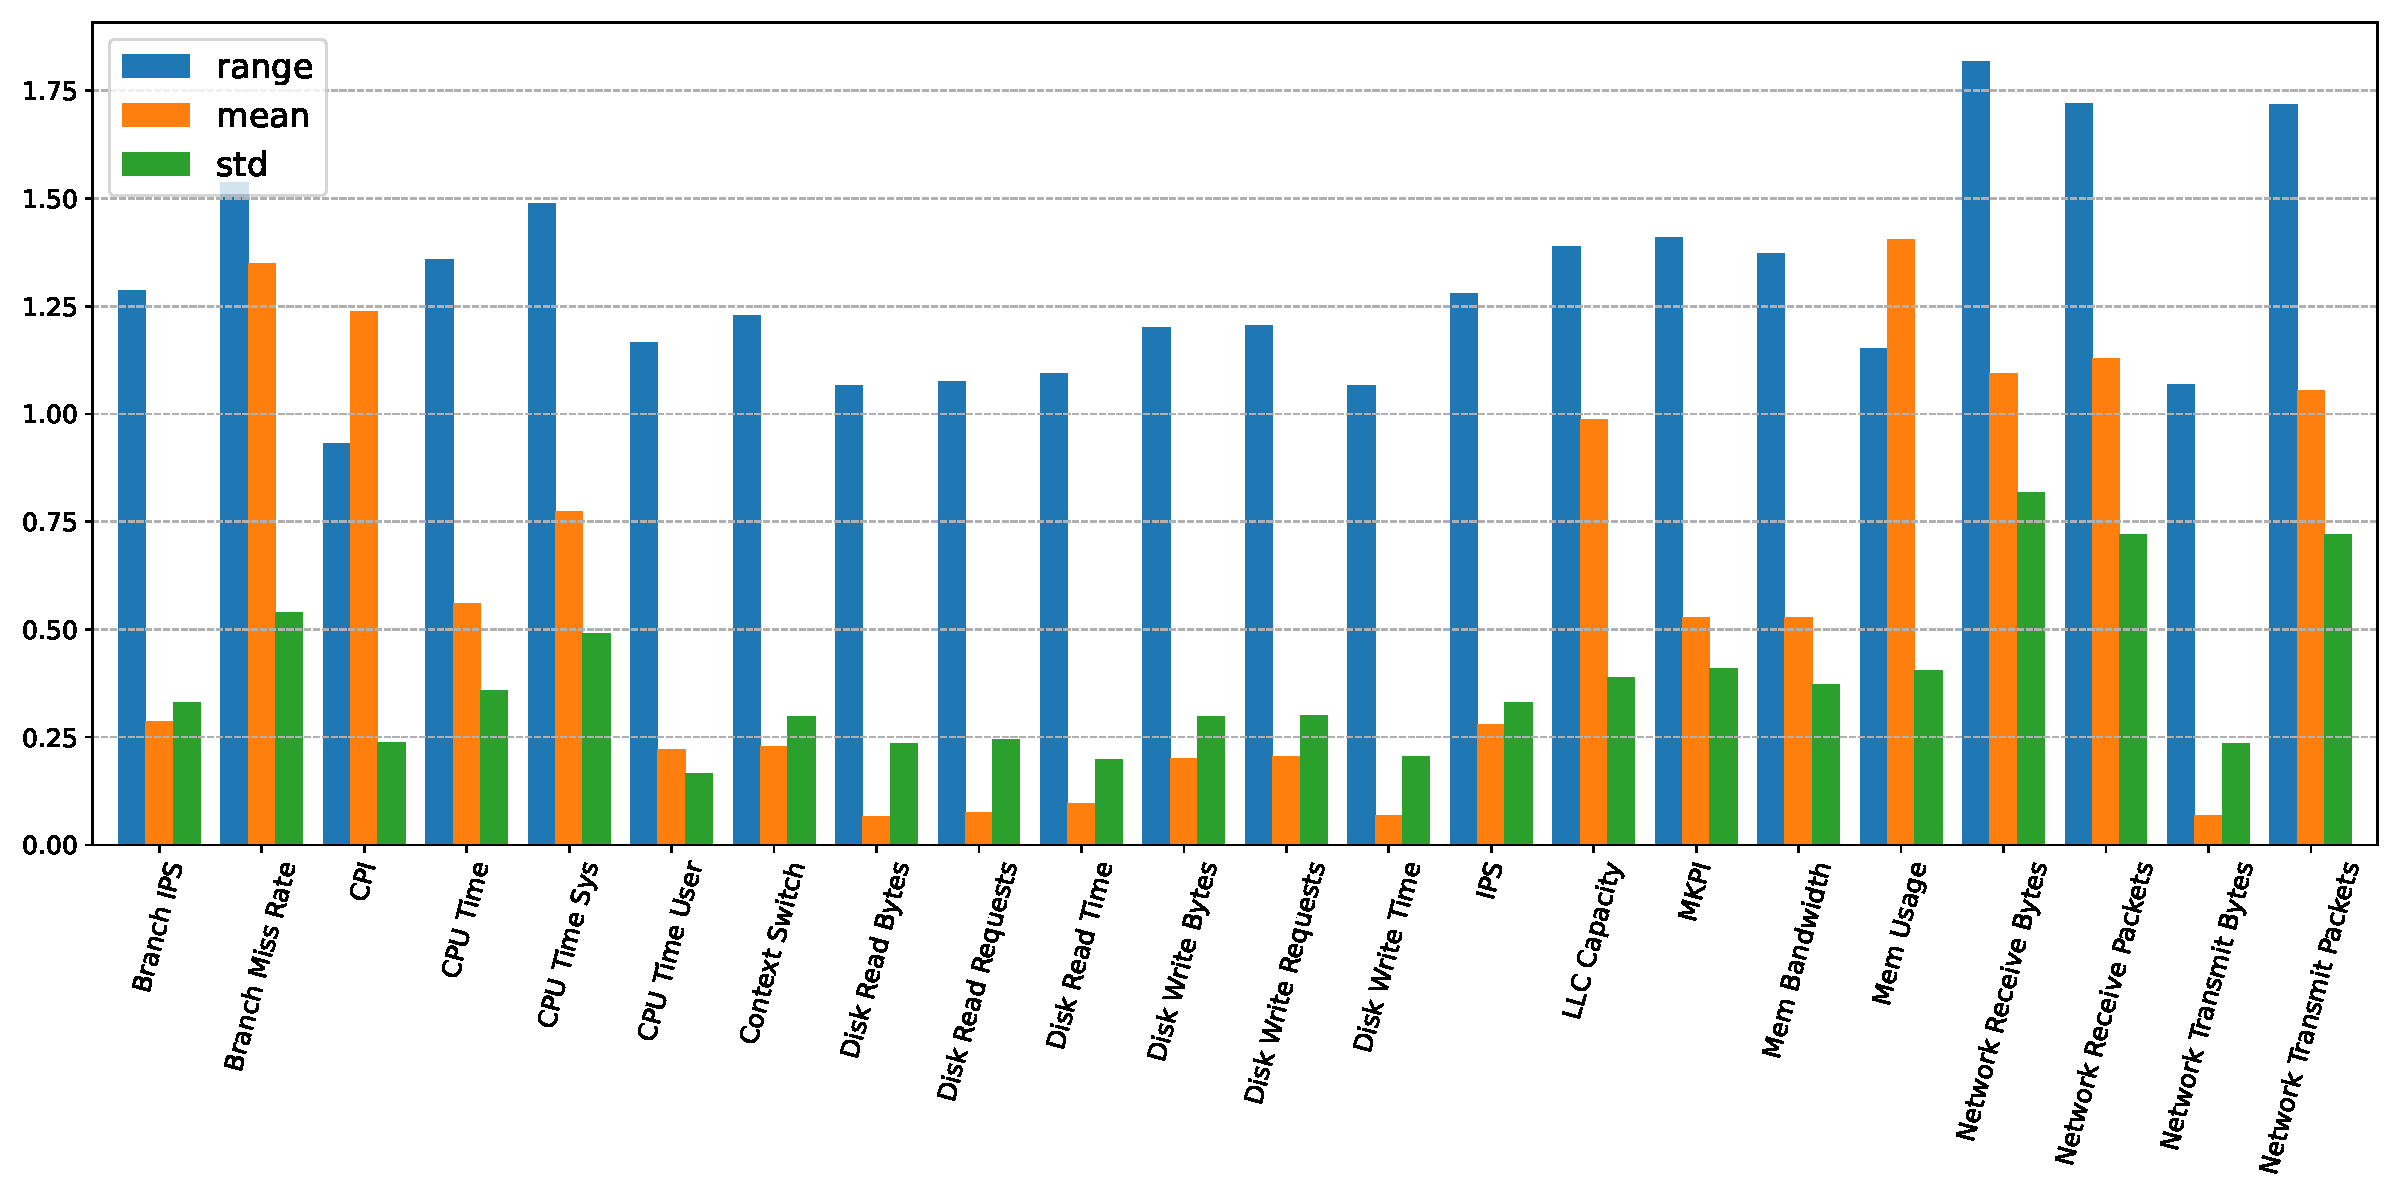
\includegraphics[width=\textwidth]{profile_kafka}
        \caption{Kafka资源使用}
        \label{fig:profile_kafka}
    \end{subfigure}
\bicaption{\quad Nginx与Kafka资源使用情况}{\quad Resource Usage of Nginx and Kafka}
\label{fig:resource_affinity_1}
\end{figure}

2)Cache资源:末级缓存资源与内存访问强相关,分析不同应用的LLC相关指标,可以将应用按访存局部性进行划分,其中Niginx属于局部性较好的应用,其在运行过程中LLC使用率波动不明显,并且LLC Miss数量较少。而对于Redis、Memcached这类键值存储型应用,局部性则与工作负载相关,在随机负载下局部性表现较差,而在模拟负载下局部性则相对较好。

3)Memory资源:内存资源区分带宽与使用量。典型应用中,Nginx在模拟负载下对内存带宽的需求较高,这点与其在Cache资源需求上的表现一致,而其余应用则采用间歇与分批的内存读取,因此不会占用过多的内存带宽。而在内存使用量上,典型应用的内存占用除自身所需外,都与工作负载相关,而在华为云的默认负载下,各个应用都会占用一定量的内存而并没有特别的规律性。

\begin{figure}[H]
    \centering
    \begin{subfigure}[b]{0.9\textwidth}
      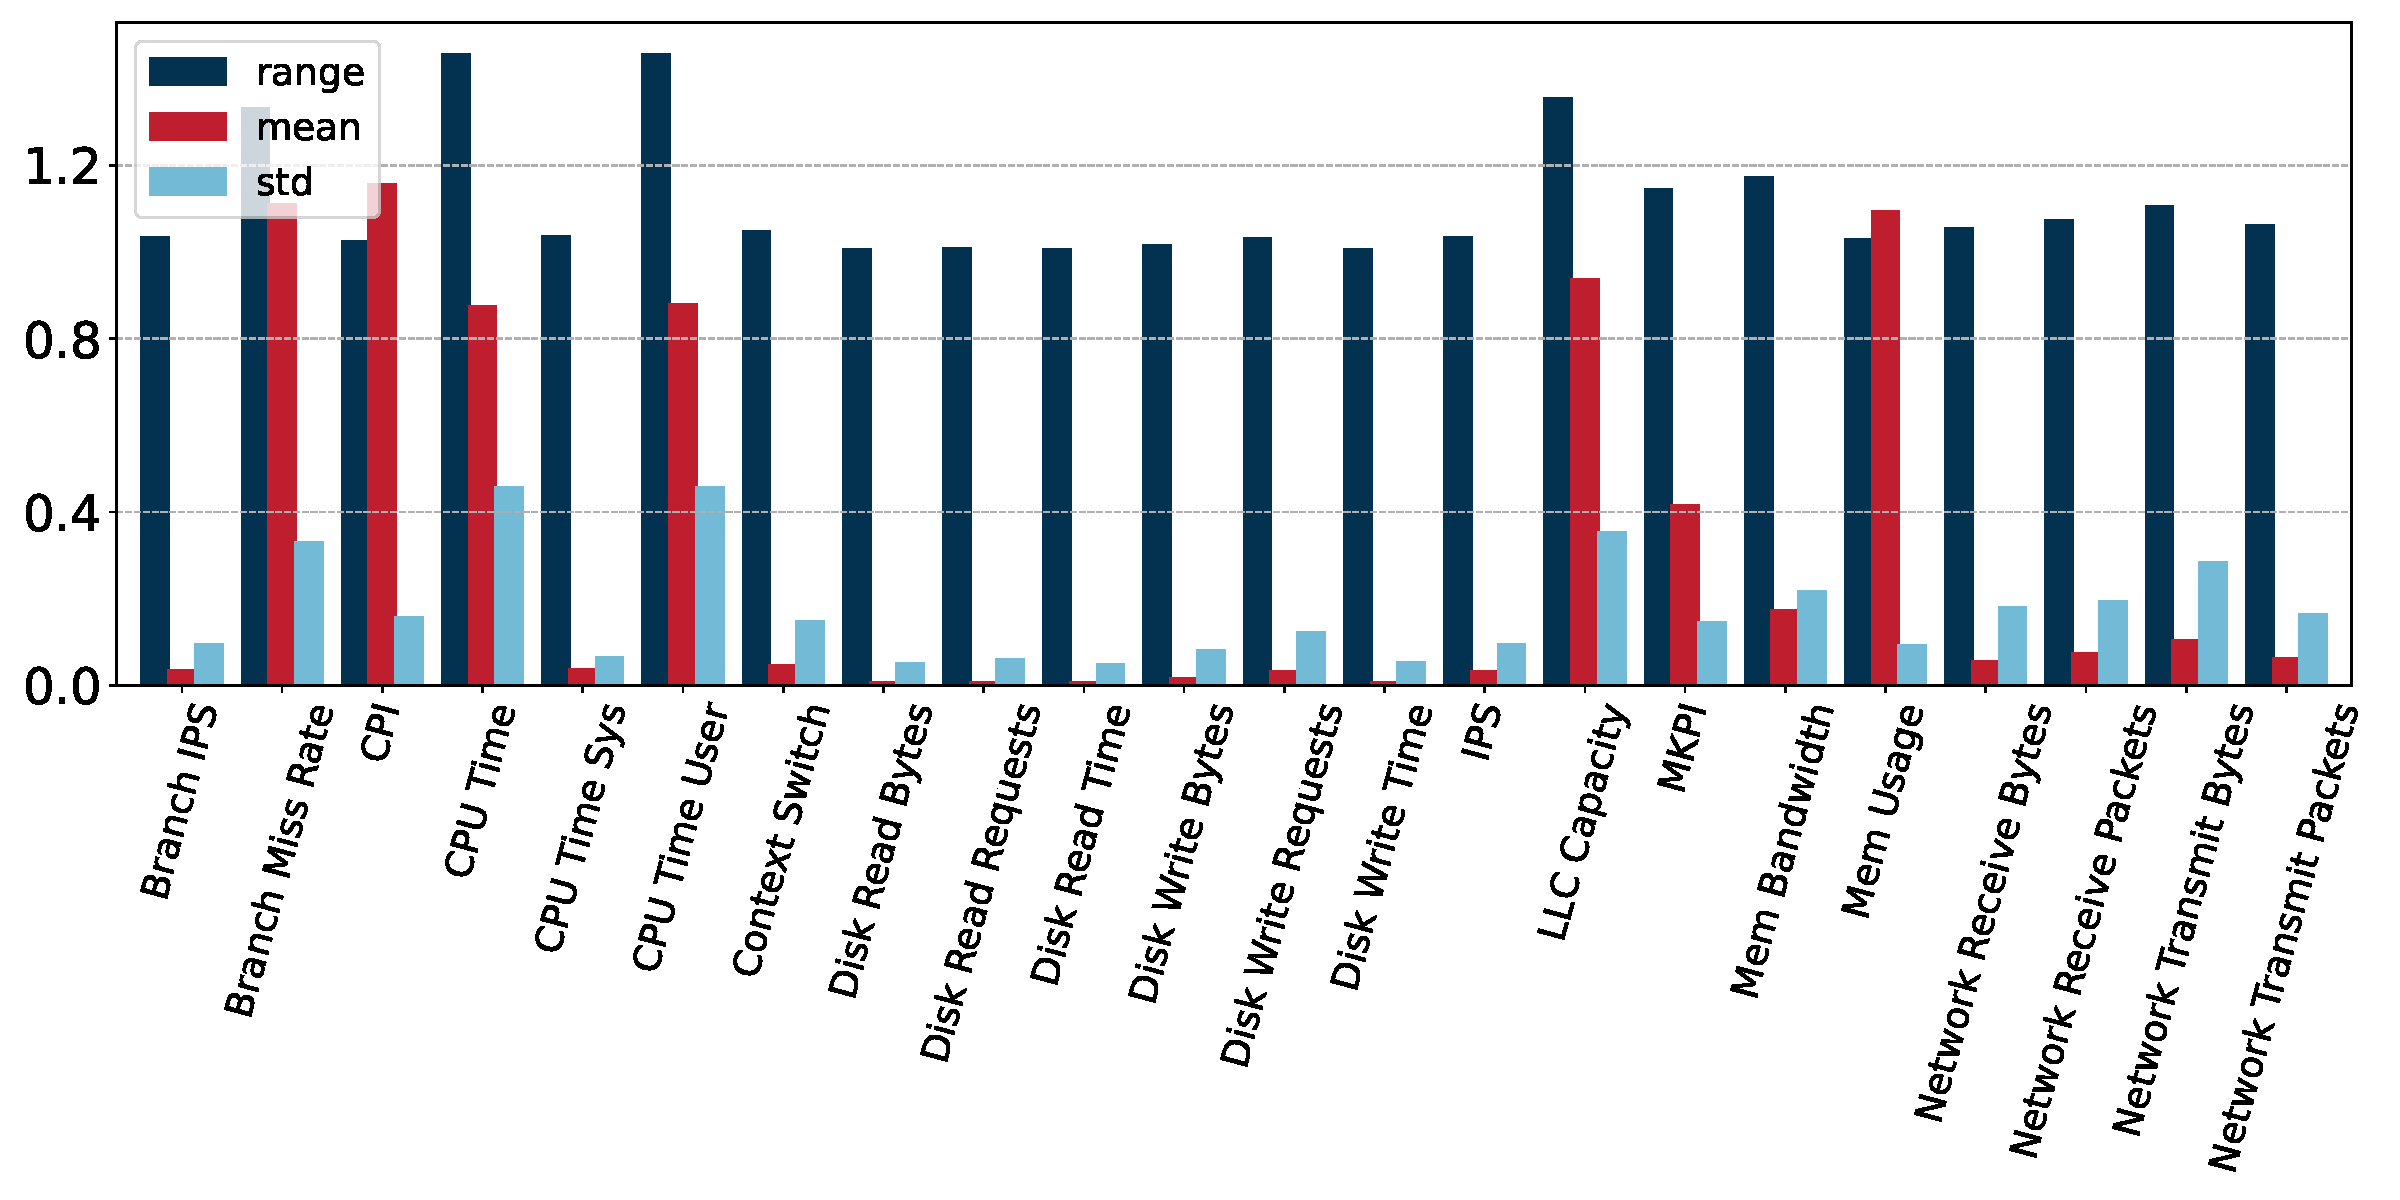
\includegraphics[width=\textwidth]{profile_elasticsearch}
      \caption{Elasticsearch资源使用}
      \label{fig:profile_elasticsearch}
    \end{subfigure}
    \begin{subfigure}[b]{0.9\textwidth}
        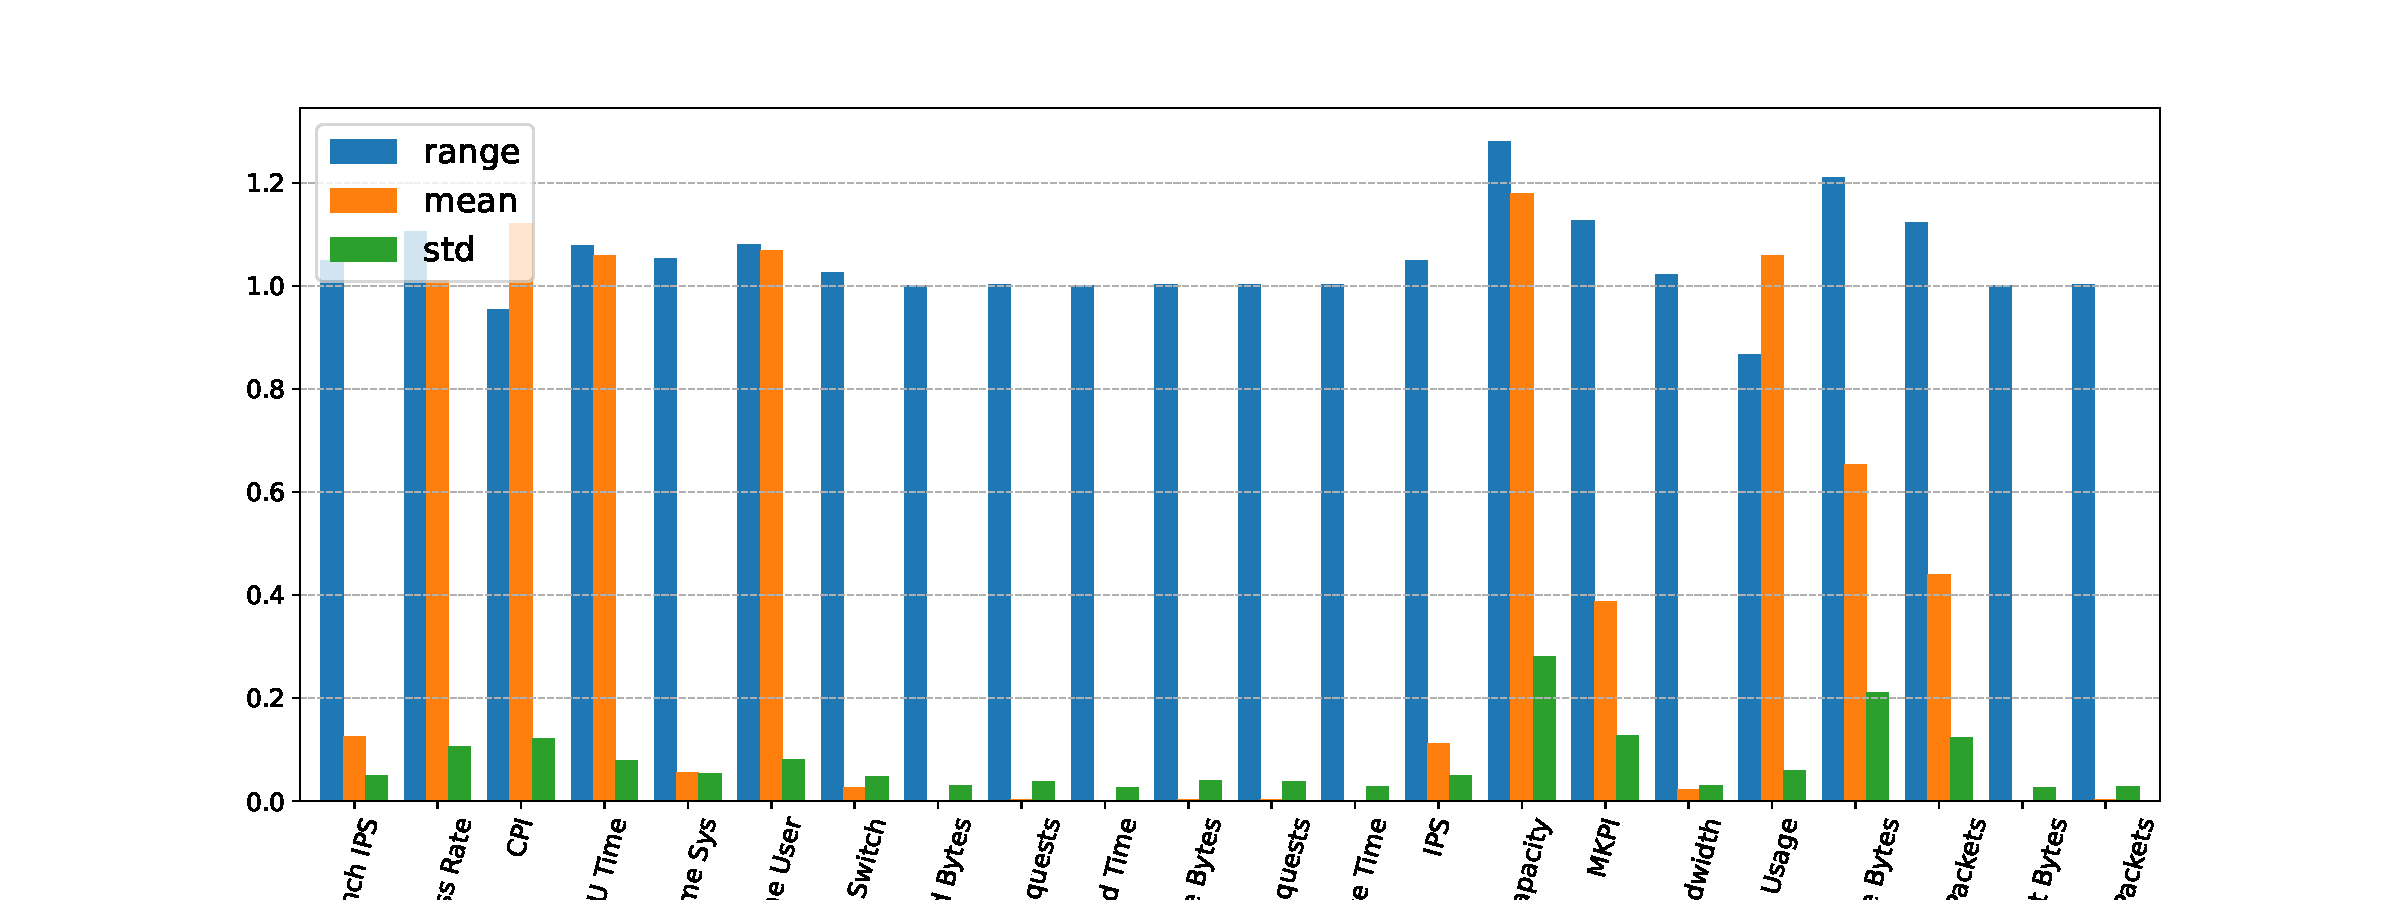
\includegraphics[width=\textwidth]{profile_render}
        \caption{Render资源使用}
        \label{fig:profile_render}
    \end{subfigure}
\bicaption{\quad Elasticsearch与Render资源使用情况}{\quad Resource Usage of Elasticsearch and Render}
\label{fig:resource_affinity_2}
\end{figure}

4)Network资源:在网络资源上,不同的应用使用需求差异很大,其中Redis、Memcached、Kafka表现出极高的网络需求,事实上这些应用都是服务型应用或自身就是网络消息中间件。而Elasticsearch、Render等在网络资源的需求上则相对较少,其中Elasticsearch并非不使用网络,而因为工作负载中并没有长时间且持续性的请求,Render则因为是离线应用,因此几乎不会使用到网络资源。

5)I/O资源:在I/O资源上,不同应用的使用需求差异同样十分大。其中Elasticsearch、Kafka和Mysql由于涉及到存储内容的持久化,因此会大量地使用I/O资源。而类似Redis等应用,虽然存在数据持久化的配置,但实际运行中持久化频率较低,因此通常只会有周期性的少量I/O资源占用。

\subsection{典型应用资源敏感度分析}

资源敏感度主要分析典型应用与不同配置下的干扰进行混部后的性能劣化情况,其中应用性能使用竖亥Benchmark提供的白盒指标进行评价。白盒指标中既有经过加权计算后的统一评分,也有对于每个应用单独的评价指标,在性能劣化中,主要选择劣化程度与干扰程度较为相关的指标进行分析。

\begin{figure}[H]
    \centering
    \begin{subfigure}[b]{0.45\textwidth}
        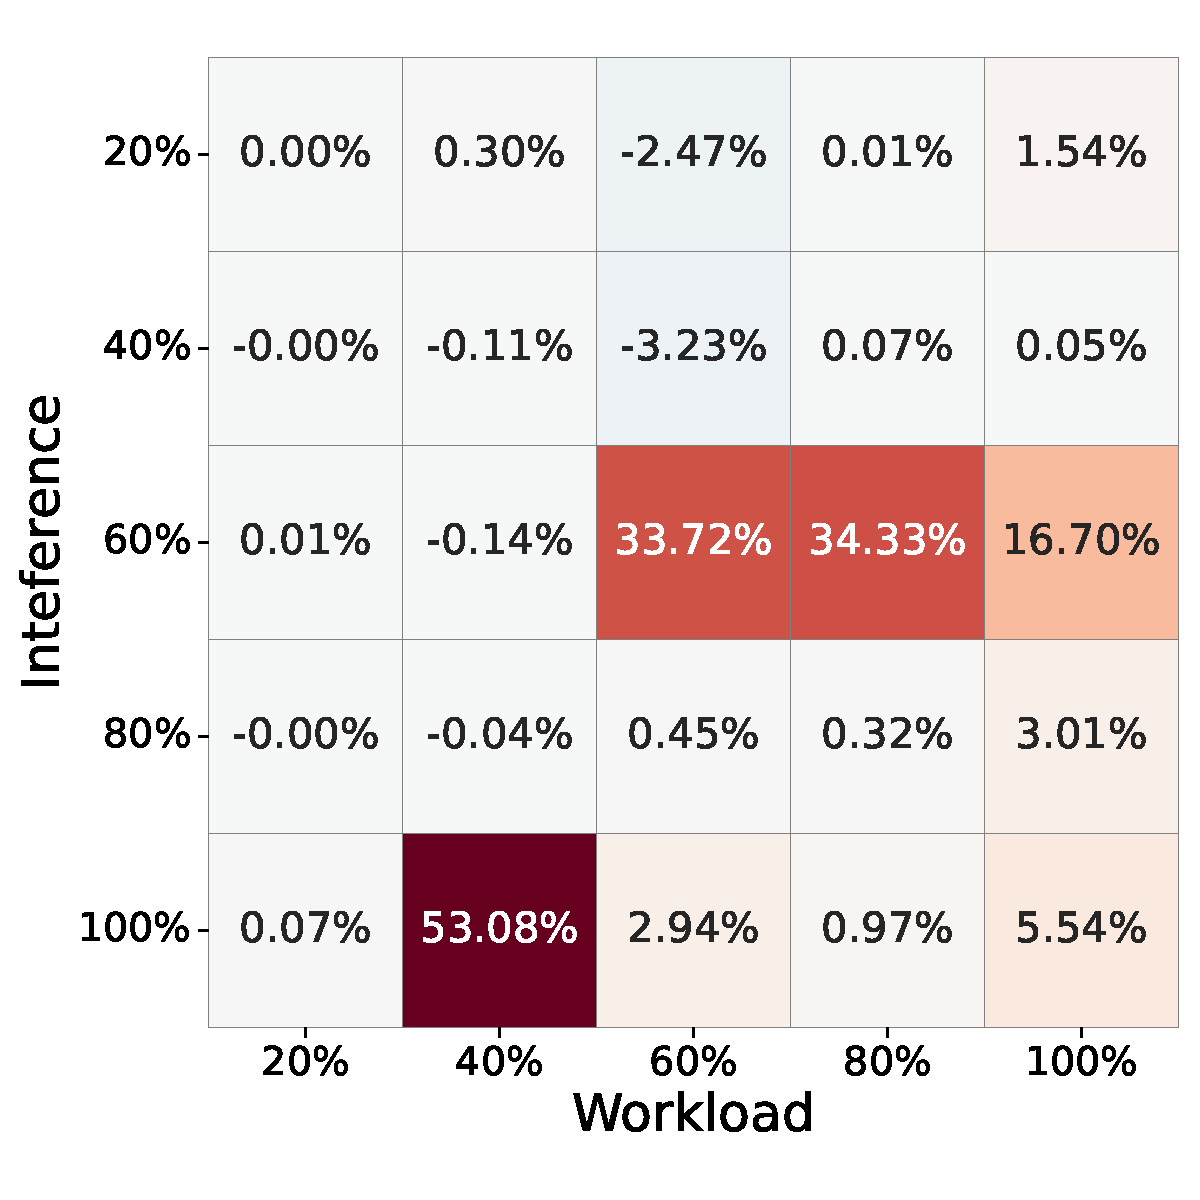
\includegraphics[width=\textwidth]{interfer_cpu}
        \caption{CPU干扰下的性能劣化情况}
        \label{fig:interfer_cpu}
    \end{subfigure}
    \begin{subfigure}[b]{0.45\textwidth}
      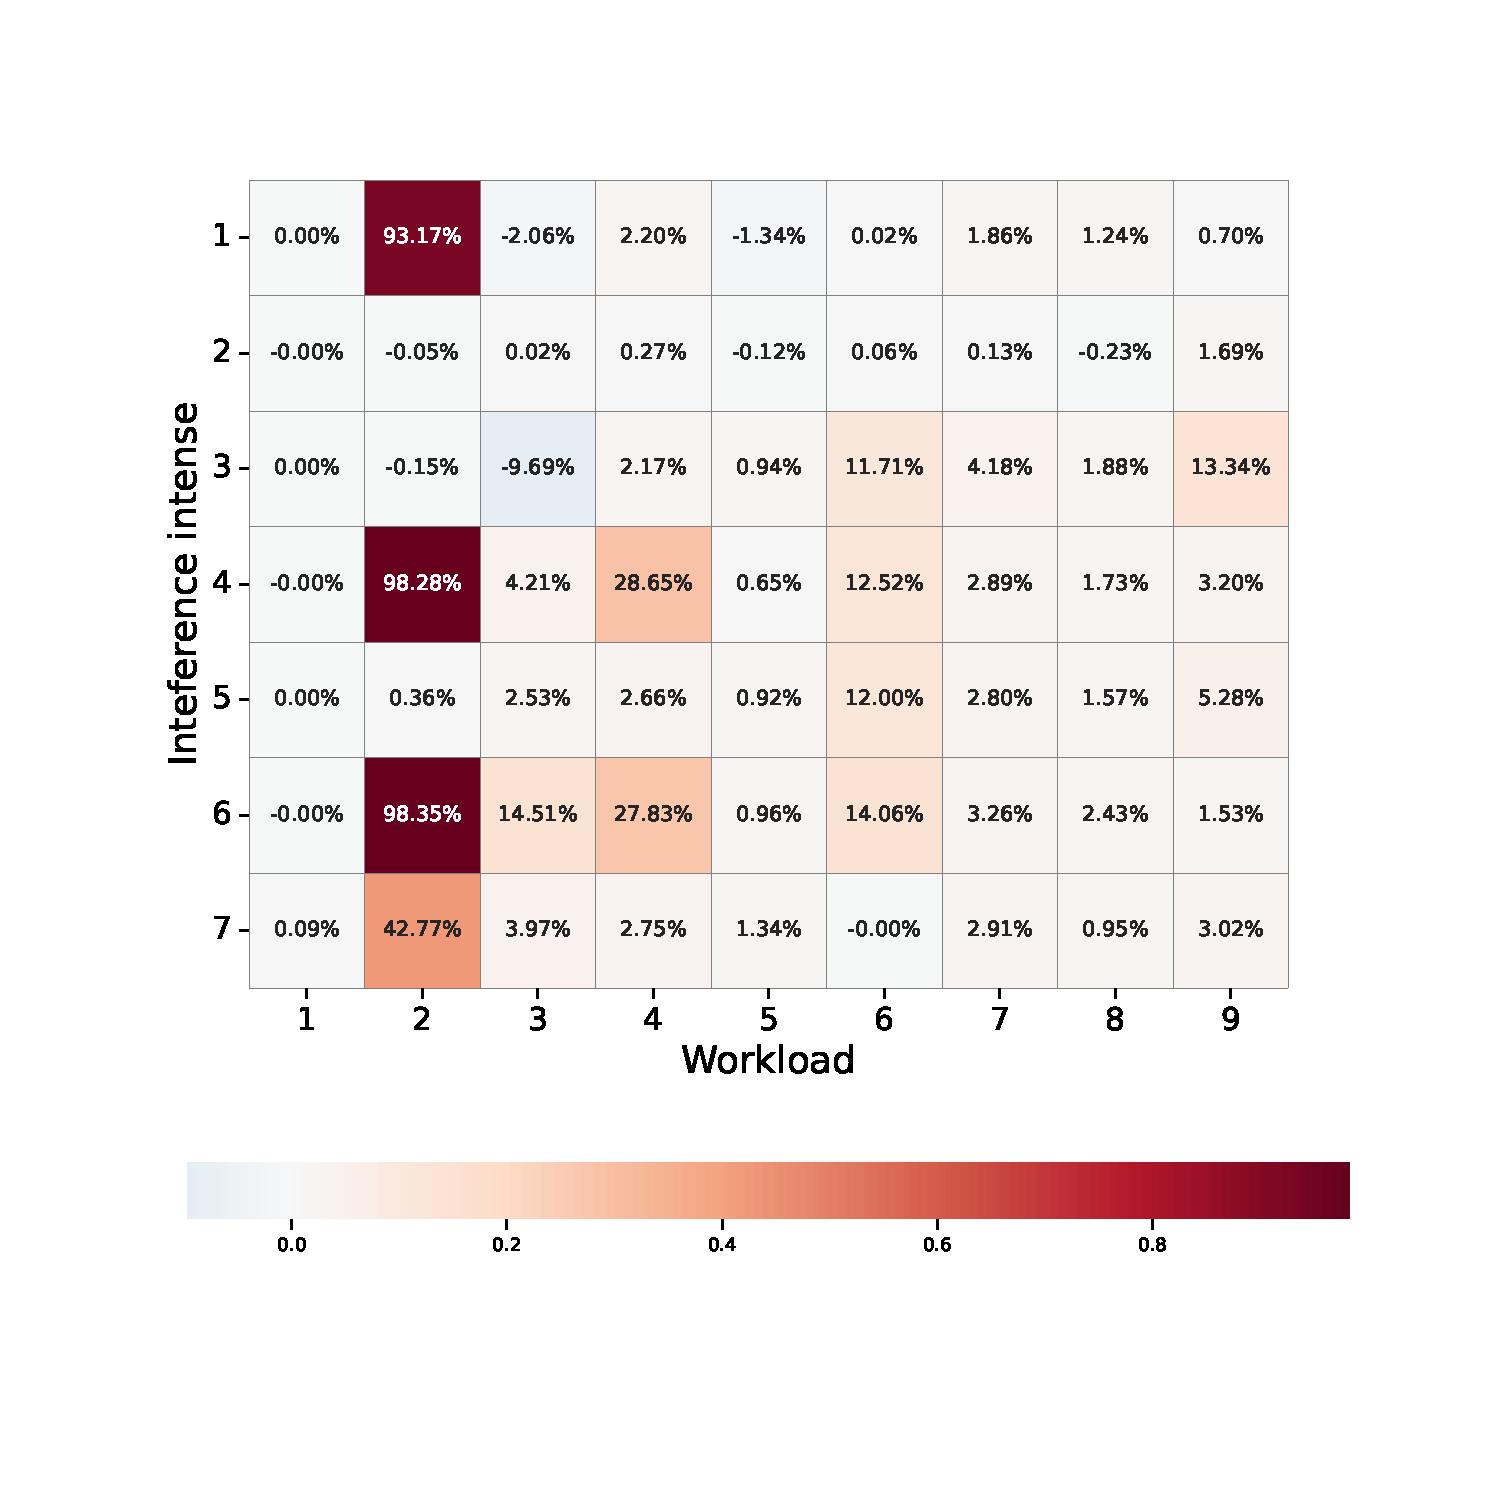
\includegraphics[width=\textwidth]{interfer_cache}
      \caption{Cache干扰下的性能劣化情况}
      \label{fig:interfer_cache}
    \end{subfigure}
    \begin{subfigure}[b]{0.45\textwidth}
        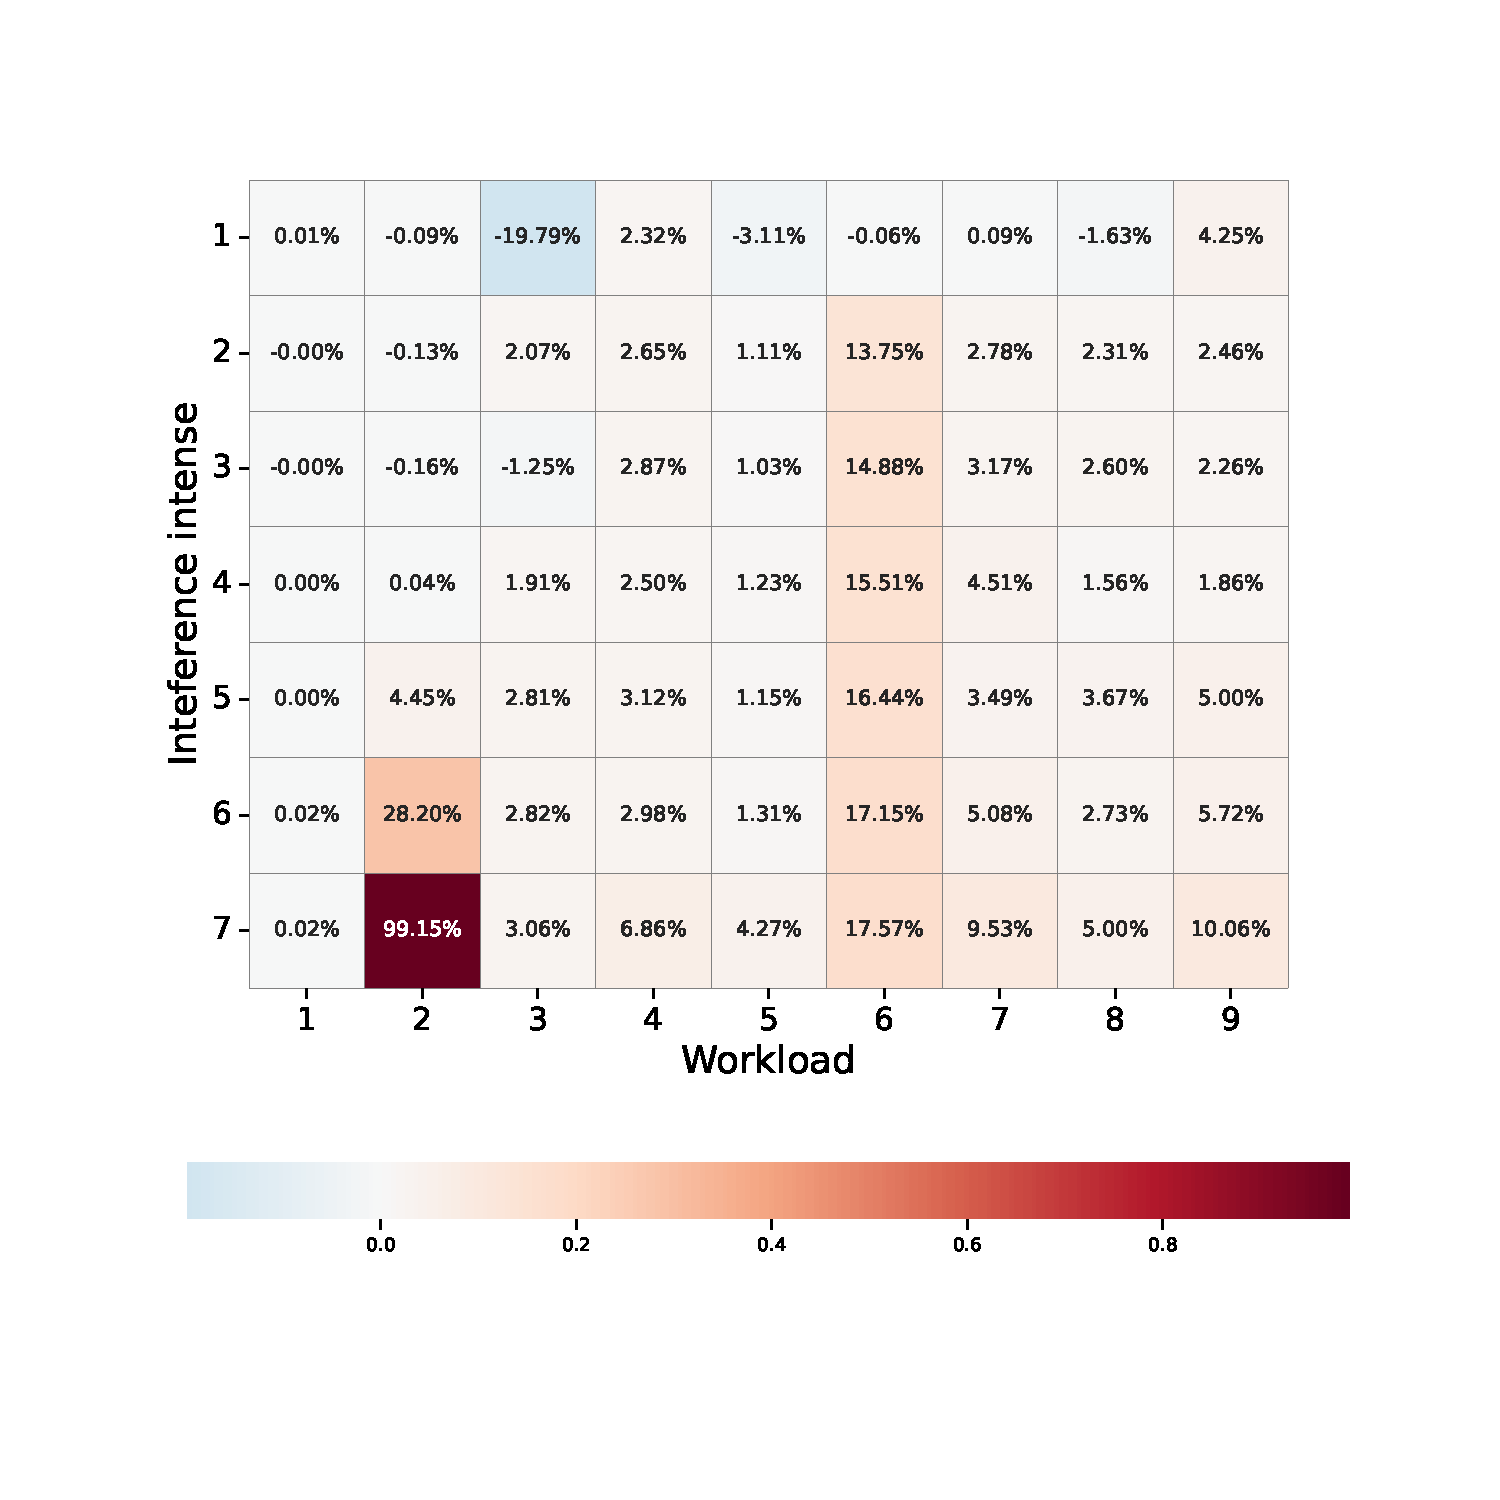
\includegraphics[width=\textwidth]{interfer_io}
        \caption{IO干扰下的性能劣化情况}
        \label{fig:interfer_io}
    \end{subfigure}
    \begin{subfigure}[b]{0.45\textwidth}
        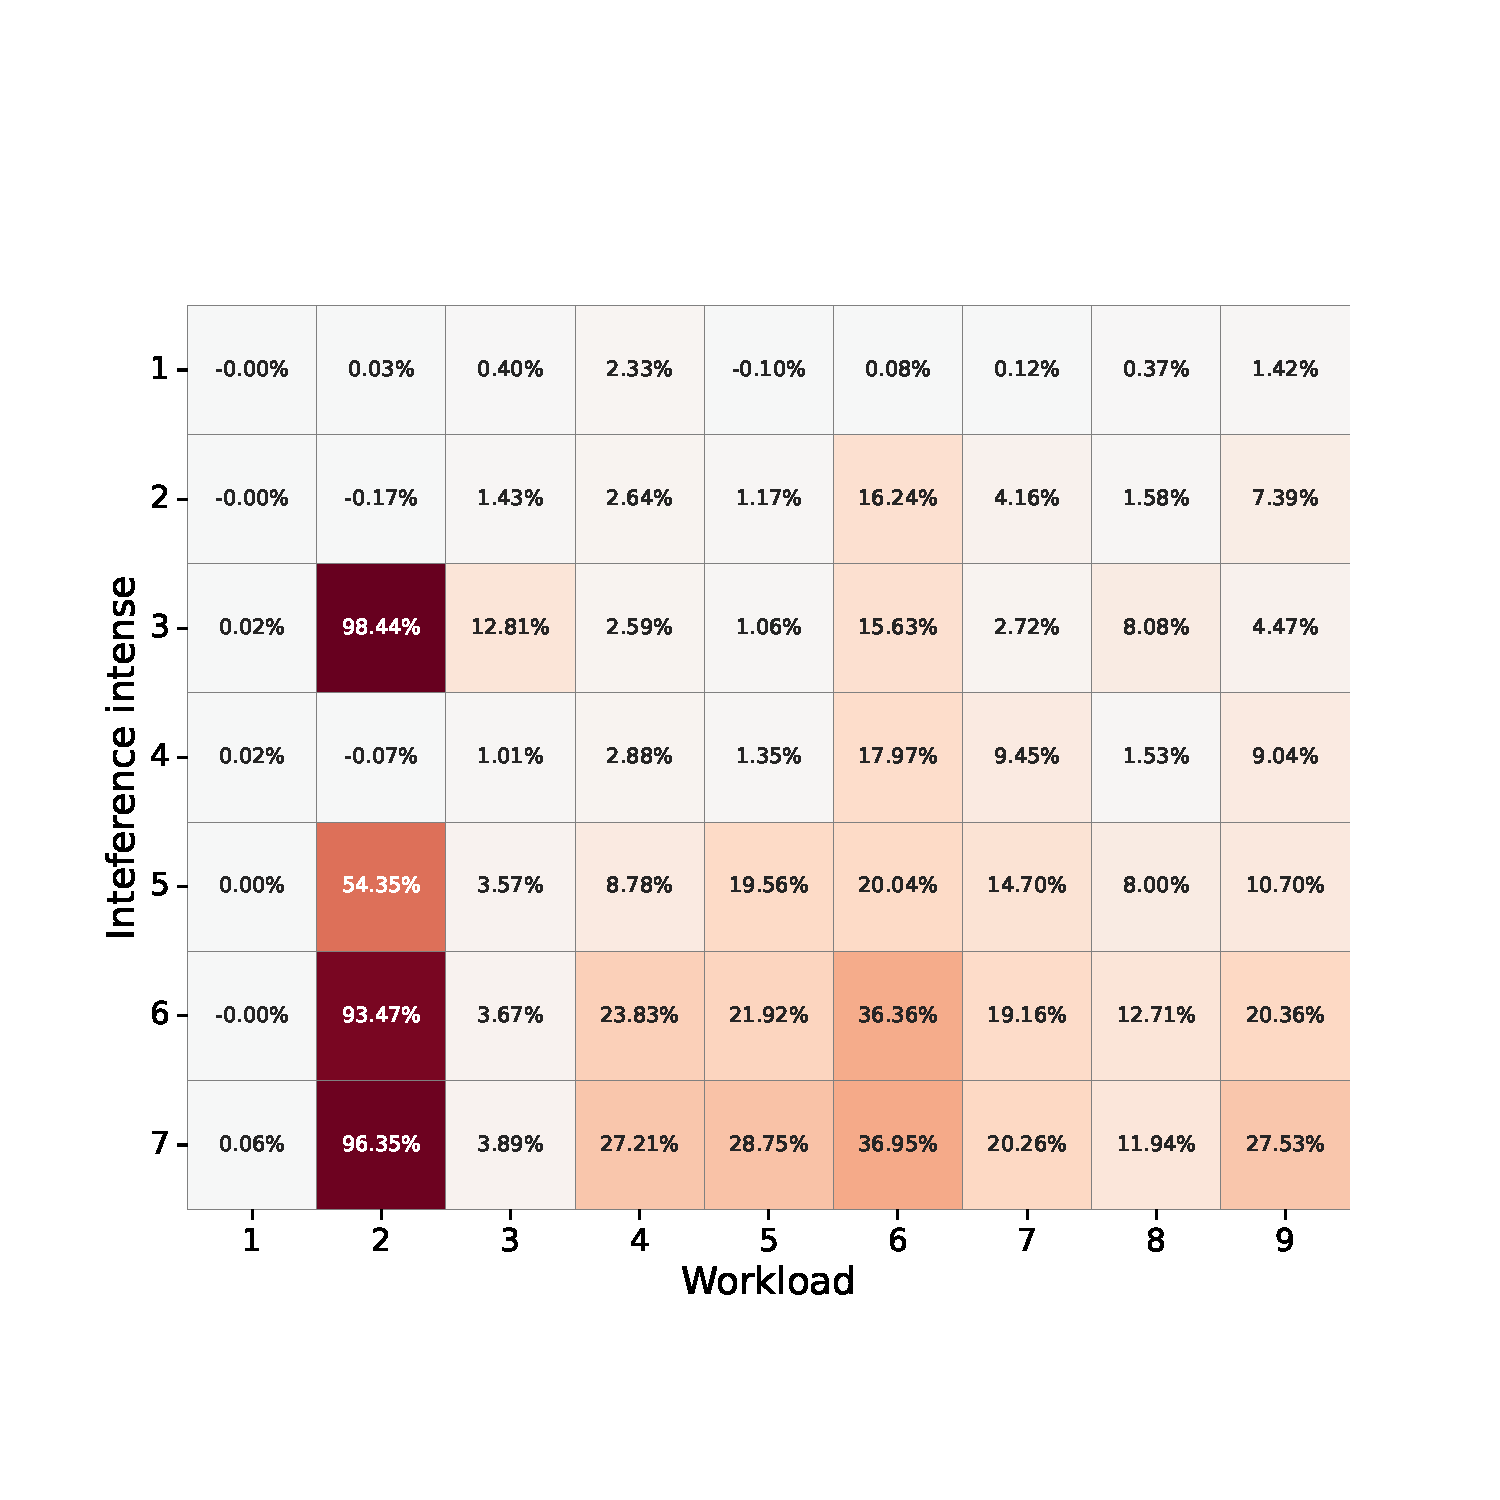
\includegraphics[width=\textwidth]{interfer_mem}
        \caption{Memory干扰下的性能劣化情况}
        \label{fig:interfer_mem}
    \end{subfigure}
\bicaption{\quad Redis干扰敏感度}{\quad Redis interference sensitivity}
\label{fig:redis_interf_sensitivity}
\end{figure}

以Redis为例,使用redis操作延迟作为性能评价指标,计算有无干扰下的指标变化百分比用于描述劣化程度,综合不同干扰及不同负载下的实验结果如图~\ref{fig:redis_interf_sensitivity}所示。

结合其他应用的资源敏感性分析,可在资源的角度对典型应用进行初步划分,主要为如下3类:

1)单纯CPU敏感型:此类应用对于CPU干扰最为敏感,而受其他干扰影响的程度则明显更低。如Memcached,其在受到CPU资源干扰后产生了近50\%的性能劣化,而对于在其他干扰下的劣化程度则在10\%内,同样的情况也在Kafka的实验数据中出现。

2)CPU与Cache敏感型:此类应用同时受CPU与Cache干扰明显,且通常对CPU干扰更加敏感。如Redis,与Memcached类似,对CPU干扰十分敏感,而同时由于Redis没有开启多线程支持,因此在Cache资源上的竞争能力弱于Memcached,从而更容易受到Cache干扰的影响。Elasticsearch情况则更为复杂,竖亥Benchmark中提供了不同的白盒指标来表征Elasticsearch的性能,主要分为吞吐量与延迟,以吞吐量作为标准,则Elasticsearch符合CPU敏感型,而以延迟作为标准,则Elasticsearch则更倾向于CPU和Cache敏感型,这种现象在其他典型应用中也有出现,而对于Elasticsearch,其使用场景中更注重吞吐量,因此在本研究中将其归类为CPU与Cache敏感型。

3)资源不敏感型:此类应用对于所有干扰的敏感度都偏低。实验中Render在各个干扰下都没有出现较为明显的劣化,这主要有两个原因。一方面,在性能指标上,Render应用使用了完成时间作为性能评价指标,而与其他应用的性能指标不同,完成时间这一指标更偏向于整个运行过程的总体性能述而不是单一处理过程的性能,一些突发的性能劣化不会体现在这一指标上,另一方面,内核调度机制上在未作限制时倾向于公平地分配时间,因此干扰程序会因调度的影响向Render出让CPU时间,而当CPU资源总和足够满足Render使用时,性能指标就不会出现较大变化。

\section{本章小结}

本章主要论述了对应用进行画像分析的过程,首先结合与云厂商的合作经验,确定了在以虚拟机为沙箱环境运行有限个应用的场景,并选取了云场景中常见的7种应用作为画像分析的对象。

然后对场景进行拆解分析,并提出了一种从Host、Hypervisor到App三个层次的协同监控机制设计,利用虚拟机本身作为进程的特殊性,串联三个维度的指标,并创新性地提出了一种基于eBPF对虚拟机监测的方式,对于本身为进程的虚拟机,监测其在系统调用上的吞吐与延时,而针对虚拟机的特殊性,则通过在虚拟化设备后端的关键路径上进行监测,实现更丰富的指标采集。

随后根据上述设计,设计实现了一套可观测性系统,除利用到开源的Promethues、Node Exporter外,还根据监控需要,实现了Libvirt Exporter、KVM Exporetr、Resctrl Exporter以及Kernel Exporter,完成所有的设计需求。

在可观测性基础设施实现完毕后,本章继续讨论实验的设计,实验围绕8种常见应用展开,并设计了有干扰实验与无干扰实验,在有干扰实验中,利用资源限制手段来减少干扰中的噪声,通过制造CPU、Cache、Memory及IO四种干扰,来分析应用对于干扰的敏感程度,而通过无干扰实验,来分析应用的资源使用倾向

最后在所有实验完成之后,分析从Prometheus中采集得到数据,来为应用进行画像分析,提供了应用的资源使用倾向及干扰敏感度评级,并探讨了除LC与BE外更多的混部机会。
% \chapter{混部场景导向的调度定制}\label{chap:sched_policy}

% Core调度框架定制(静态) -> Control Tower任务调度框架定制(动态) -> 资源感知调度机制定制(动态) -> 资源感知调度策略定制(动态) 

为解决不同混部场景下任务调度机制的不足,本章主要展开混部场景导向的定制任务调度机制研究。首先,从内核任务调度的相关配置上,针对不同应用的需求,设计了响应度优先与吞吐量优先两种基础内核配置,随后,在Sched Ext项目的基础上设计场景导向的Control Tower任务调度框架,并在此基础上结合eBPF的监测能力,进一步设计了CPU资源感知与网络资源感知的任务调度策略。

\section{内核调度配置定制}

Linux调度子系统提供了一些编译配置选项,用以针对场景进行优化,相关配置选项围绕时钟中断与抢占模型展开。

时钟中断是驱动Linux抢占式调度的核心机制,如表~\ref{tab:config_hz}所示,Linux内核提供了时钟中断频率与时钟中断处理模式两方面的配置。其中,中断的频率配置决定了调度滴答的周期,Linux提供了从100、250、300到1000四种不同的中断频率配置,一方面,越高的时钟中断频率意味着系统的整体响应度更好,另一方面,因此越高的时钟中断频率意味着更准确的时间记账。Linux在时钟中断处进行时间记账,但实际运行过程中,由于中断间隔可能存在任务切换,因此时间记账并不一定准确。时钟中断频率决定了时间片的最小粒度,而越高的时钟中断频率意味着越小的时钟中断间隔,同时在间隔中发生任务切换的概率也会越小,从而能够实现更准确的时间记账。

\begin{table}[H]
    \bicaption{\quad 内核时钟中断配置}{\quad Kernel Clock Interrupt Configuration}% caption
    \label{tab:config_hz}
    \footnotesize% fontsize
    \setlength{\tabcolsep}{4pt}% column separation
    \renewcommand{\arraystretch}{1.25}% row space 
    \centering
    \begin{tabular}{lc}
        \hline
        配置名称 & 描述 \\
        \hline
        HZ\_100  & 配置时钟中断频率为100  \\
        HZ\_250  & 配置时钟中断频率为250 \\
        HZ\_300  & 配置时钟中断频率为300 \\
        HZ\_1000 & 配置时钟中断频率为1000 \\
        HZ\_PERIODIC & 永远不要忽略时钟中断 \\
        NO\_HZ\_IDLE & 忽略空闲CPU上的时钟中断 \\
        NO\_HZ\_FULL & 忽略空闲CPU,以及只有一个可运行任务CPU上的时钟中断 \\
        \hline
    \end{tabular}
\end{table}

时钟中断会打断当前任务的执行,并产生上下文切换的开销,为此Linux内核提供了如表~\ref{tab:config_hz}所示的不同时钟中断处理模式,来减少特定场景中不必要的时钟中断开销。相关配置的核心时NO\_HZ配置。在开启NO\_HZ选项之后,Linux内核允许指定部分CPU核心为NO\_HZ核心,这些CPU核心会根据不同的时钟中断处理模式,在如CPU空闲等特定场景下,忽略时钟中断以实现节能、减少对任务干扰的目的。

抢占通常指高优先级任务打断低优先级任务的执行。Linux内核中,用户态任务总是会被中断抢占,而对于内核态任务,则处理手段有所不同。在早期Linux内核实现时,通常会在内核态任务执行时屏蔽中断,此时一些较长的内核处理路径中就会引发系统整体的响应度下降。为此内核提供了如表~\ref{tab:config_preempt}所示的四种抢占模型,用于配置内核代码执行时对中断的处理模式。不同抢占模式的主要区别在于内核代码中可被抢占位点,内核代码中可被抢占的位点越多,系统的实时性通常就会越好,但也意味着任务的执行更容易被频繁地打断,因此需要根据不同应用的需要来进行选择。

\begin{table}
    \bicaption{\quad 内核抢占模式配置}{\quad Kernel Preemption Configuration}% caption
    \label{tab:config_preempt}
    \footnotesize% fontsize
    \setlength{\tabcolsep}{4pt}% column separation
    \renewcommand{\arraystretch}{1.25}% row space 
    \centering
    \begin{tabular}{lc}
        \hline
        配置名称 & 描述 \\
        \hline
        PREEMPT\_NONE  & 内核代码保持执行直到主动放弃CPU  \\
        PREEMPT\_VOLUNTARY  & 开启了内核代码中的抢占位点 \\
        PREEMPT  & 提供更多的内核代码抢占位点,实现完全抢占 \\
        PREEMPT\_RT & 进一步修改内核代码的实现,如锁机制,实现实时可抢占性 \\
        \hline
    \end{tabular}
\end{table}

时钟中断和抢占模式配置共同决定了Linux调度子系统的整体响应度,根据应用的不同需求,本文设计了响应度优先与吞吐量优先两种基本调度子系统内核配置。其中,响应度优先配置采用更高的HZ与激进的抢占模式来提升整体响应度,满足应用对于延迟与实时性的需求。吞吐量优先配置则采用较低的HZ与保守的抢占模式,让CPU在有限的时间内更多的执行任务而不是处理时钟中断,从而满足应用对于局部性和CPU资源的需求。

\section{Control Tower任务调度框架设计}

% 混部Linux优先级机制的问题
% - 调度队列优先级问题: 
%  - 优先级机制用于限制不同任务对CPU时间的使用,并不能保证高优先级的应用一定能够比低优先级应用优先调度
% - 调度类优先级问题:
%  - 运行在实时调度类中的LC任务如配置不当,一方面不利于应用性能,另一方面容易造成系统崩溃
%  - 将低优先级的任务允许在Idle类是嵌入式领域的常用做法,但不够灵活,且违背Linux设计语义
% 解决方式
% - 引入Ext调度类,使能调度队列隔离
% - 利用BPF Scheduler的灵活性
% 调度器架构
% - User Input: Task define, Resource define
% - eBPF Input: Task status, Resource status
% - Control Signals: BPF Map、BPF Prog: rodata\bss
% - BPF Scheduler: Select Eligible Task to Eligible CPU
% - Control: BPF Helper \ User Define Command \ eBPF Define
% 调度模式
%  - 全局调度
%  - Per-CPU调度
% 调度策略
%  - FIFO
%  - RR
%  - Vtime

混部场景中使用优先级机制来保障高优先应用QoS是常用的手段,Linux提供了调度类与调度队列两层的优先级定义,然而在应用的QoS上保障上两层优先级的机制都存在一定的不足。

在调度类层,利用调度类的优先级差异能够保证高优先就绪时总是能够抢占低优先应用,从而实现高优先应用的QoS保障。优先级差异可以通过将高优先应用添加到较高优先级的调度类,或者将低优先应用添加到低优先级调度类实现。将高优先应用添加到高优先级调度类时,需要充分考虑应用的特点与高优先级调度类的配置,不恰当的配置一方面会影响应用本身的性能,另一方面也有可能引发整个系统性能下降。将低优先任务添加到低优先级调度类,如Idle调度类时也存在风险。首先,将常规任务放置到Idle调度类破坏了Idle调度类的设计语义,不利于系统能耗。其次,Idle调度机制十分基础,无法满足不同低优先任务的调度需求。

在调度队列层,以默认的CFS调度为例,CFS提供从-20到20的静态优先级,能够影响应用vruntime的积累速度。高优先应用的vruntime相对增加得缓慢,通常能够得到更多的调度机会,但是随高优先应用的vruntime不断累积,在CFS公平调度的机制实现下,存在在被低优先应用抢占的可能。同时,CFS调度器中包含了许多不利于高优先应用QoS保障的启发式逻辑。CFS的执行过程中会为每个调度队列维护一个基准的vruntime,通常是调度队列中vruntime的最小值,新创建和刚唤醒的进程会被赋予基准vruntime值,并在CFS调度算法下得到优先执行。然而,这一启发式逻辑没有考虑到进程之间的优先级,当低优先级大量唤醒或创建时,高优先应用反而会被频繁抢占并产生QoS劣化。其次,调度队列层优先级无法跨CPU地产生作用,这一方面导致高优先应用与运行在其他CPU上的低优先应用争抢资源,另一方面使得高优先应用在不同CPU上迁移时相对优先级变化而导致优先性丧失。

为解决混部场景下Linux任务调度在QoS保障上的问题,本文设计了Control Tower任务调度框架,能够在保障高优先任务全局优先性的同时支持灵活的调度策略。Control Tower任务调度框架基于Sched Ext项目设计。引入Ext调度类的目标首先在于解决Linux任务调度机制中的优先级问题。Ext调度类处于Fair调度类与Idle调度类之间,将低优先任务添加到Ext调度类中可构建调度类优先级差异,从而实现高优先应用就绪时总是能够抢占低优先应用。同时,由于调度类优先级是系统全局的,因此能够在各个CPU以及跨机器迁移时生效。

其次,针对不同混部场景下应用的不同需求,Control Tower任务调度框架能够针对性地设计调度策略,从而根据实际情况更好地进行高优先任务的QoS保障。Control Tower任务调度框架如图~\ref{fig:bpf_scheduler_arch}所示,框架的核心是BPF调度策略,基于Ext提供的接口实现,能够定制Ext调度类的任务调度行为。除此之外,本文向BPF调度策略引入了额外的数据输入源,包括用户与其他子系统的数据输入。额外的输入数据通过BPF Map等机制提供给BPF调度策略,用以辅助进行调度决策。同时BPF调度策略也能够通过共享内存的方式将数据提供给用户态程序,并借助与用户态程序的协作实现更灵活的任务调度。

\begin{figure}[H]
    \centering
    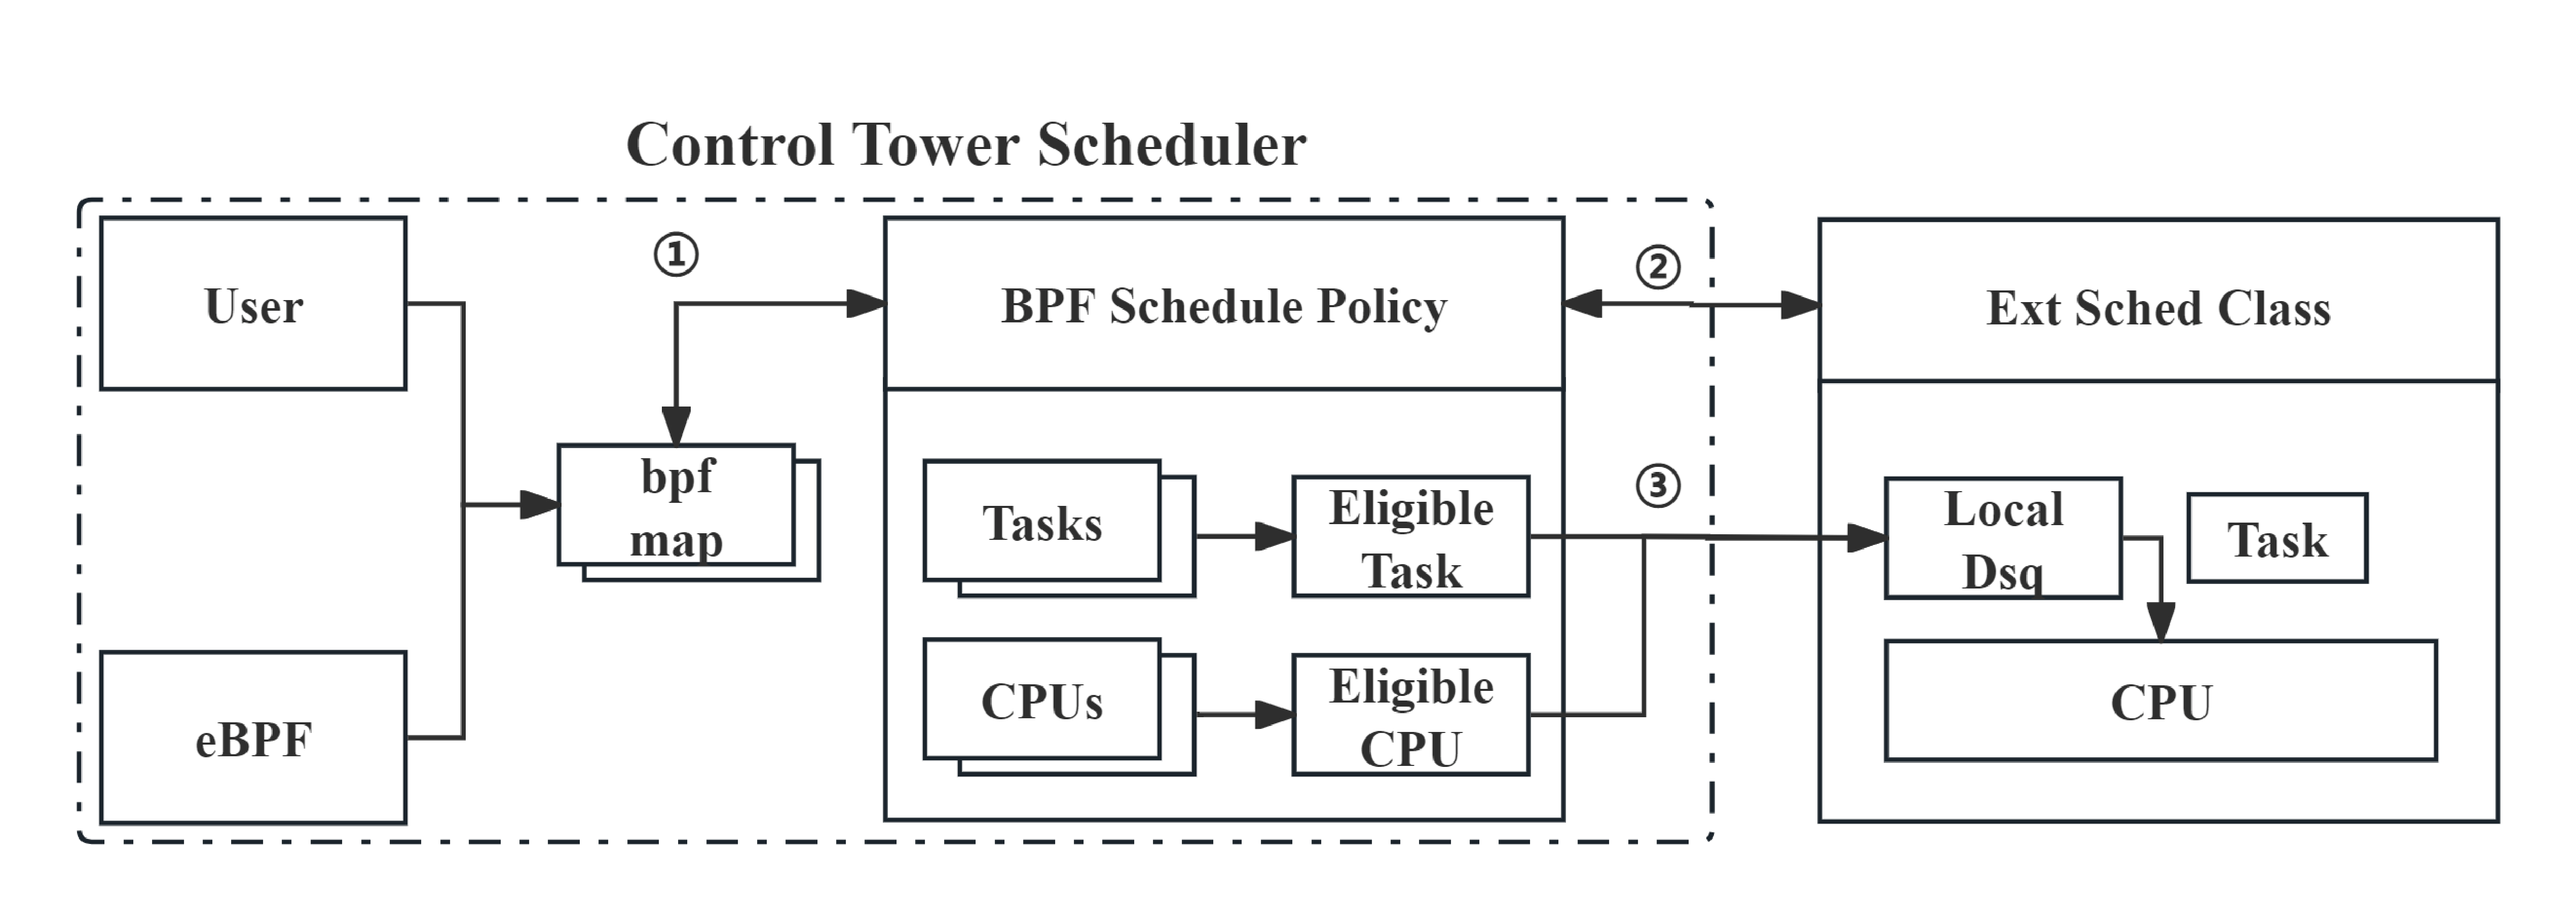
\includegraphics[width=0.9\textwidth]{bpf_scheduler_arch}
    \bicaption{\quad Control Tower任务调度框架}{\quad Control Tower scheduling framework}
    \label{fig:bpf_scheduler_arch}
\end{figure}

Control Tower任务调度框架支持用户与eBPF外部数据源。区别于Ext调度类提供的调度信息,外部数据源的信息可以由用户自定义或从其他子系统中采集。其中,用户数据源作用在BPF调度策略初始化和运行时。初始化时,用户可定义CPU资源拓扑、BPF调度策略参数等,并通过修改BPF程序的rodata、bss段来将静态信息传递给BPF调度策略。策略运行时,用户程序可以通过读写BPF调度策略预先声明BPF Pin Map来与BPF调度策略交互,如传递用户对进程、Cgroup的优先级、类型、资源需求等声明。eBPF外部数据源基于其他子系统中插桩实现,包括内核资源分配、系统调用等关键路径上,这些数据可以直接通过BPF Map共享给BPF调度策略,同时,在不同的混部场景中,eBPF插桩也可以根据需要自由选择与定制。

BPF调度策略既可以直接定制Ext调度行为,也可以在调度过程中利用上述的额外数据源来针对性地调整调度行为,同时,BPF调度策略也可以通过BPF Map来将调度信息共享给用户程序与其他子系统,从而利用用户程序的灵活性以及eBPF对如网络子系统的定制能力。Control Tower任务调度框架提供了两种基本调度模式和三种可选的调度策略。

% TODO: 调度模式图 a \ b

\begin{figure}[!htbp]
    \centering
    \begin{subfigure}[b]{0.49\textwidth}
        
\includegraphics[width=\textwidth]{bpf_per_cpu}
        \caption{Per-CPU调度模式}
        \label{fig:bpf_per_cpu}
    \end{subfigure}
    \begin{subfigure}[b]{0.49\textwidth}
        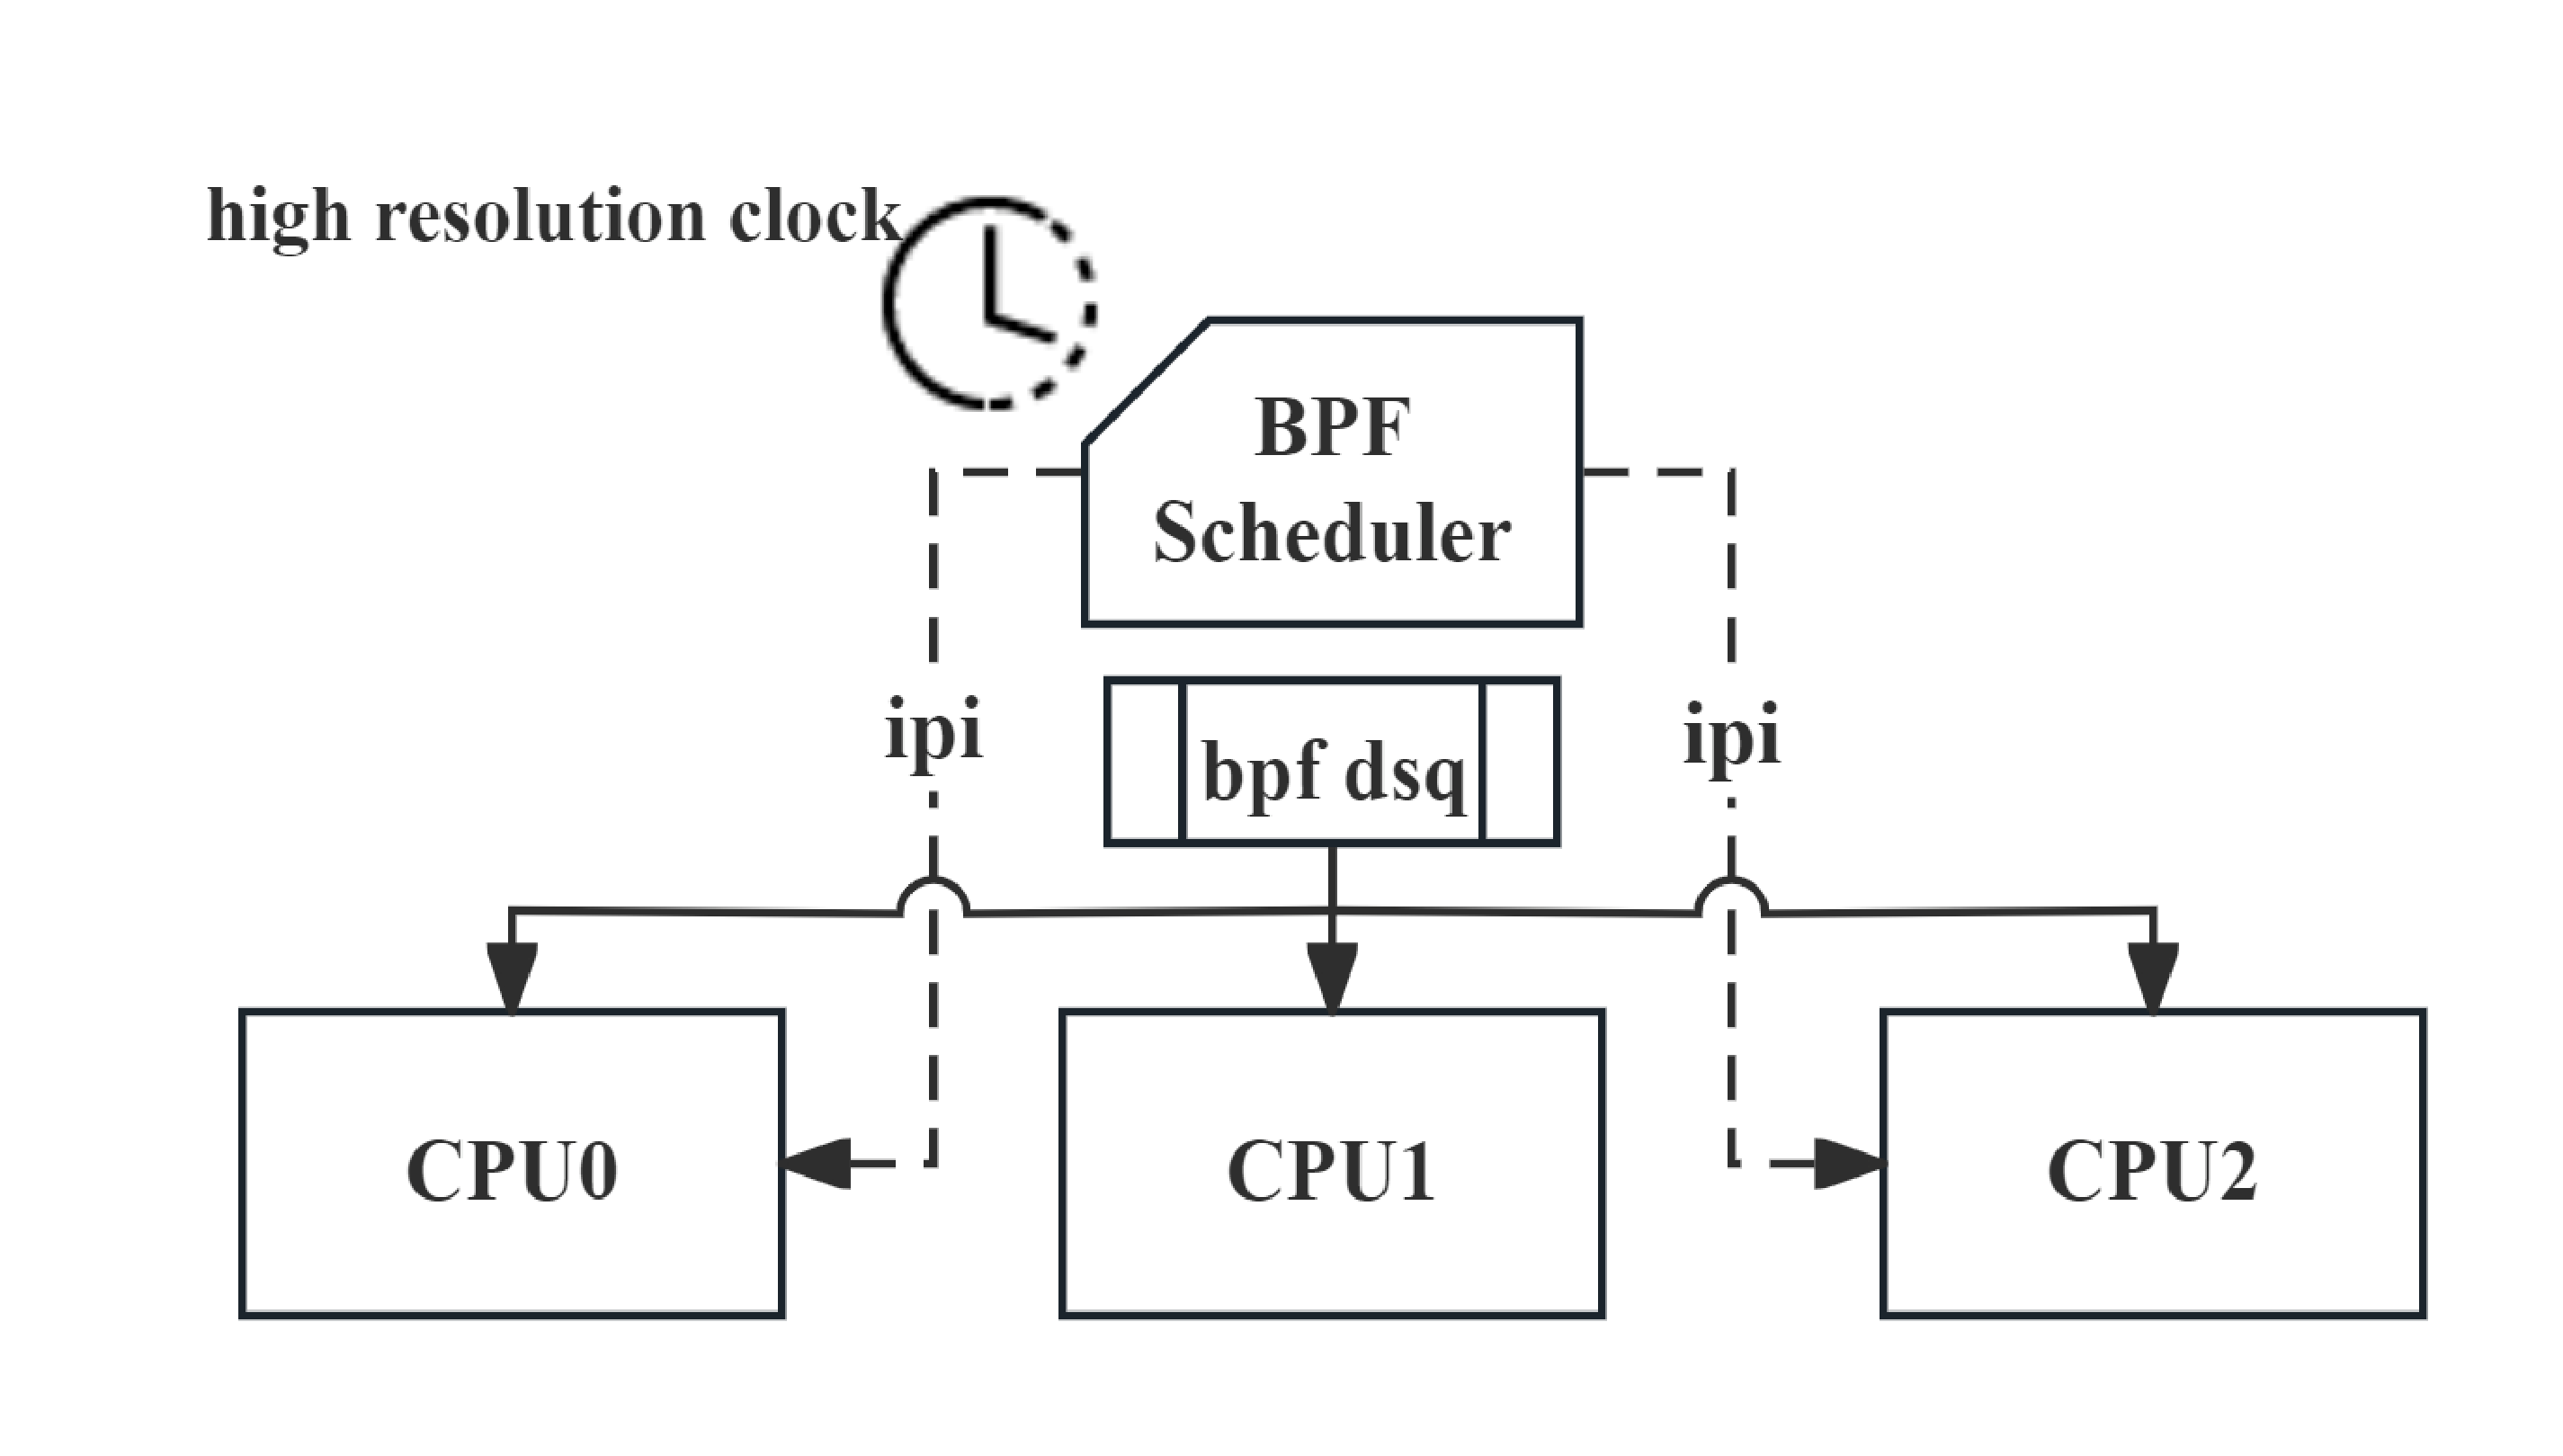
\includegraphics[width=\textwidth]{bpf_global}
        \caption{全局调度模式}
        \label{fig:bpf_global}
    \end{subfigure}
\bicaption{\quad BPF任务调度模式}{\quad BPF task scheduling mode}
\label{fig:bpf_sched_mode}
\end{figure}

在调度模式上,如图~\ref{fig:bpf_sched_mode}所示,Control Tower任务调度框架支持Per-CPU调度与全局调度两种调度模式。其中,Per-CPU调度是Linux中常用的调度模式,核心在于将调度卸载到各个CPU上来避免共享内存导致的竞争。如图~\ref{fig:bpf_per_cpu}所示,BPF调度框架中通过为每个CPU创建一个BPF DSQ,并将调度策略限制在本地CPU的BPF DSQ上来实现Per-CPU调度。Per-CPU调度模式适用于CPU数量较多且对调度开销要求较高的场景。在延时敏感的混部场景中,将调度延时降低到应用的延时阈值内是保障QoS的一种方式,受限于内核的HZ配置,Per-CPU调度延时最小为1ms(1000HZ),同时,由于Linux HZ配置是全局的,而较高的时钟中断会导致整个系统中时钟中断处理的资源使用增大,影响CPU敏感任务的执行。而为解决调度延时的问题,Control Tower任务调度框架提供了全局调度模式。如图~\ref{fig:bpf_global}所示,全局调度模式基于全局调度队列与高精度时钟实现,与其他研究类似,首先选择一个CPU作为调度核心,并在这个CPU上创建全局的DSQ。同时,在调度核心上设置一个BPF Timer,利用高精度时钟实现ns级的调度周期。全局调度模式的调度过程中,首先将新创建的任务加入到全局DSQ上,每次BPF Timer的回调中,调度核心会更新任务的记账信息并尝试调度任务,并抢占时间片耗尽的任务,其中调度核心与其他核心的交互通过IPI实现。

在调度策略上,为适应不同混部应用的调度需求,BPF调度框架提供了三种基本的调度策略实现:

\begin{enumerate}
    \item \textbf{基于FIFO的非抢占式调度}:BPF调度策略中使用FIFO DSQ(分发队列),并设置每个入队任务的时间片为无限,任务运行直到主动退出,随后BPF调度策略取出下一个任务执行。
    \item \textbf{基于RR的抢占式调度}:BPF调度策略中使用FIFO DSQ, 并按照配置设置每个入队任务的时间片,每次时钟滴答时检查当前任务的剩余时间片,抢占时间片耗尽的任务并切换到下一个任务执行。
    \item \textbf{基于vtime的抢占式调度}:BPF调度策略中使用vtime DSQ,vtime DSQ按照vtime大小对任务进行排序,初始时设置每个入队任务的初始vtime,并在每个时钟滴答里根据任务的静态优先级更新vtime,并进行抢占判断。当抢占发生时,vtime越小的任务越优先被调度。
\end{enumerate}

相较于Linux任务调度机制,Control Tower任务调度框架能够提供更灵活的任务调度机制与调控手段,并通过定制和组合不同的外部数据来源、调度模式与调度策略来满足不同混部场景应用对调度机制的需求,从而更好地保障高优先应用的QoS。

\section{Control Tower资源感知任务调度}

% 对于CPU资源的隔离,常见的方式是显示地隔离不同应用能够使用的CPU,这种静态的划分方式并不能有效的使用资源,而在本章中提出了基于BPF调度器的调度队列隔离,高低优先级的应用在调度队列优先级机制之上共享相同CPU,使得高优先级应用运行时总是能够优先地使用CPU资源。

% 其次,相较于常见的调度类隔离,本章基于BPF调度器实现更为灵活,通过结合eBPF强大的监测能力,让BPF调度器感知高优先级应用CPU资源、网络资源的使用,而通过设置相关的资源约束,从而结合不同高优先级应用的资源使用特征与调度目标,更充分的利用资源。

\subsection{CPU资源感知的任务调度} 

% 进行CPU资源隔离的原因
% CPU Set静态资源划分的问题
% CPU资源感知机制的实现
% - 用户定义的CPU拓扑
% - Ext调度类eBPF hook
% CPU资源感知策略的实现
% - 保守调度场景
% - SMT场景 

CPU拓扑描述了CPU之间的资源共享情况,而CPU之间的资源共享是混部场景中“吵闹邻居”的核心原因,这要求调度需要考虑CPU间的拓扑关系。使用CPU Affinity机制将不同应用划分到不同的CPU集合中是常用方式,然而这种方式存在一些缺陷。首先,CPU Affinity隔离粒度较粗,划分不当容易造成CPU资源浪费。其次,静态的CPU集合划分没有考虑到应用CPU资源使用的动态特性,较保守的策略容易造成资源浪费,而激进的策略则容易引发QoS劣化。

造成上述问题的核心在于划分CPU集合时并没有考虑到不同应用对CPU资源的实际使用情况,而为解决这一问题,本文设计了CPU资源感知的任务调度策略,调度逻辑如伪代码~\ref{alg:cpu_aware_sched}所示,通过增加外部数据源的方式,让低优先任务感知高优先应用使用CPU资源的情况,并结合用户输入的CPU拓扑判断是否需要出让CPU资源,从而实现高优先应用的QoS保障。

CPU资源感知的任务调度策略基于Control Tower任务调度框架实现。首先,在BPF程序初始化时,用户需要传入当前系统CPU拓扑以及低优先任务所能使用的CPU数量。随后,BPF程序初始化过程中会创建一个全局数组记录Ext调度类所管理的CPU状态,并通过在Ext调度类cpu\_acquire与cpu\_release处的插桩动态更新。任务调度时,BPF调度策略读取全局数组,计算得到当前低优先任务能够使用的CPU数量,并与阈值进行比较。当不满足CPU阈值时,拒绝进行任务调度,而目标CPU会在Local DSQ没有任务执行时,出让CPU并被Idle调度类抢占。而当CPU满足阈值时,BPF调度策略首先将任务调度到目标CPU的Local DSQ上,并根据目标CPU的状态来决定是否需要发送IPI。

\begin{algorithm}[H]
    \caption{Pseudocode for Enhanced Task Scheduling Isolation Mechanism}
    \label{alg:cpu_aware_sched}
    \begin{algorithmic}[1]
    
    \Function{cpuAcquire} {cpu}
    \State Insert cpu to CPU\_Map;
    \EndFunction
    
    \Function{cpuRelease} {cpu}
    \State Remove cpu from CPU\_Map;
    \EndFunction
    
    \Function {schedule}{}
        \While{True}
            \If{$\text{CPU\_Acquired + CPU\_Idle} < \text{CPU\_Available}$ }
                \State Set Exclusive Flag;
                \For{each no\_hz core C}
                    \State Send an IPI to envoke target CPU rescheduling.
                \EndFor
                \State Yield to higher priority scheduler class;
            \EndIf
            \State Remove Exclusive Flag;
            \State Dispatched tasks;
        \EndWhile
    \EndFunction
    \end{algorithmic}
\end{algorithm}

Control Tower任务调度框架提供了以调度队列为粒度的CPU资源划分,相较于CPU Affinity粒度更细。借助调度类优先级差异,低优先任务能够在高优先任务运行时及时出让CPU资源,从而实现动态的CPU资源分配。然而这种资源的出让没有考虑CPU的拓扑关系,在如SMT作为底层硬件的混部场景中,无法有效地保障高优先应用的QoS。而CPU资源感知任务调度策略通过用户输入以及CPU资源的eBPF探测弥补了这一缺陷,能够更好地在SMT以及激进的高优先任务QoS保障场景中发挥作用。

\subsection{网络资源感知的任务调度}

% 网络资源感知的目标
% - 现有问题
% 网络资源感知机制的实现
% - Epoll系统调用eBPF hook
% - LC应用划分
% 网络资源感知策略的实现
% - LC应用低负载,高负载,负载高时,基于Epoll的LC应用特征变化(CPU敏感),要求吞吐量
% - 交还eevdf, 动态时间片

混部场景中LC应用通常为网络服务应用,在画像分析中发现,网络服务应用的资源使用倾向与敏感度在不同负载下存在差异。在负载较低时,由于请求量少、处理时间快,因此对资源的需求不高,且受到干扰影响不明显。而在负载较高时,对资源的需求激增,同时干扰会导致处理请求的速度变慢,而待处理请求的积压会引发较大QoS劣化。

高性能网络应用通常使用epoll作为底层的网络机制。epoll允许进程同时监听多个连接,并在连接就绪时进行批量处理,相较于阻塞型网络系统调用,使用epoll能够在大量请求时减少频繁地阻塞唤醒过程,从而支持更高的并发量。epoll机制涉及到多个系统调用,而其中最为核心的是epoll\_wait系统调用,进程在注册等待事件之后,就能够通过epoll\_wait系统调用来获取当前的就绪事件,当存在就绪事件时,epoll\_wait系统调用会返回就绪的事件数量,而当没有事件就绪时,epoll\_wait仍然会阻塞进程。

实际生产环境中,网络服务应用的负载更加具有波动性,然而,Linux任务调度机制并不考虑混部应用在不同负载对于调度需求,同时也缺乏有效的应用负载感知机制。为解决上述问题,本文设计了网络资源感知的任务调度策略,调度逻辑如伪代码~\ref{alg:network_aware_sched}所示,通过eBPF插桩获取应用的实时负载,并从用户输入获取目标应用在不同负载下的调度需求,并针对性地实施不同的调度策略,在低负载下以系统吞吐为目标,而在高负载时以高优先应用的QoS保障为目标。

\begin{algorithm}[H]
    \caption{Pseudocode for Network Resource Constraints Scheduling Strategy}
    \label{alg:network_aware_sched}
    \begin{algorithmic}[1]

    \Function {do\_epoll\_wait\_return}{$nr\_event$}
        \State Write timestamp of current epoll wait;
        \State Write $nr\_event$ of current epoll wait;
        \State Update total event count;
        \State Update count of epoll wait;
    \EndFunction

    \Function {schedule}{}
        \While{True}
            \State Read epoll wait delta from bpf map;
            \If{$\text{EPOLL\_WAIT\_DELTA} < \text{EPOLL\_WAIT\_THRESHOLD}$ }
                \State Set Exclusive Flag;
                \For{each no\_hz core C}
                    \State Send an IPI to envoke a rescheduling;
                \EndFor
                \State Yield to higher priority scheduler class;
            \EndIf
            \State Remove Exclusive Flag;
            \State Dispatched tasks;
        \EndWhile
    \EndFunction
    \end{algorithmic}
\end{algorithm}

网络资源感知调度策略增加了基于epoll\_wait系统调用探测的eBPF数据源。具体eBPF代码中,首先创建两个Per-CPU BPF Map,分别记录Per-CPU上epoll\_wait系统的频率与事件数量,同时在key的选择上,支持pid、Cgroup以及系统三种监测粒度。而在eBPF插桩位点上,选择do\_epoll\_wait内核函数的返回位点,此处不仅表示一次epoll\_wait系统调用的完成,也能够通读取返回值,获取此次epoll\_wait系统调用所得到的epoll事件数量。每次计数完毕后,都会更新此次计数的时间戳,结合计数与时间戳数据,就能够计算应用的负载量。

网络资源感知调度策略在Control Tower调度框架中的实现也有多种方式。首先,BPF调度策略可以在调度时,参考高优先应用的负载情况,在低负载时,直接调度任务而不考虑CPU拓扑上的资源竞争,并调节时间片大小,在满足高优先低负载时的基本延时需求的同时,实现更高的系统吞吐。而在高负载时,采用避让的原则,减少与高优先应用的资源竞争,从而实现高优先应用的QoS保障。其次,也可以将探测逻辑与BPF调度策略分离,如在低负载时,关闭BPF调度策略,此时低优先任务会被Fair调度类调度,并与高优先应用处在相同的调度队列中,通过分时复用进一步提高吞吐,而在高负载时,加载CPU资源感知的BPF调度策略,并设置较为保守的参数来优先保障高优先应用的QoS。

% \subsection{基于PMU实现的其他资源感知策略}

\section{实验设计与分析}

\subsection{响应度优先内核性能}

% redis \ memcached

响应度优先任务调度配置使用HZ\_1000配置时钟中断频率,并配置PREEMPT抢占模式。实验在4 CPU、1024MB内存的虚拟机上展开,选择Redis、Memcached、Nginx和Mysql四种延迟敏感应用来分别与stress\_ng CPU干扰应用进行混部,并与HZ\_250和VOLUNTARY抢占模式的CloudHV默认Linux内核比较。

混部实验结果如图~\ref{fig:perf_response}所示,响应度优先内核配置几乎在所有混部场景下都实现了更好的应用QoS保障。对于业务逻辑较简单的LC应用,如Redis、Memcached与Nginx,响应度优先内核分别实现降低99分位尾延迟最高39.2\%、36.9\%、35.2\%的效果。高响应度的配置能够及时地为LC应用分配CPU资源,避免请求的积压从而保障应用的延时需求。MySQL混部实验中响应度优先内核能在一定程度上提升MySQL的事务处理能力。但由于MySQL线程数多、业务逻辑复杂,在较高负载时,由于NO\_HZ核心配置多线程下失效,频繁的时钟中断也导致执行有效任务的时间减少,使得MySQL的延时上升。

\begin{figure}[H]
    \centering
    \begin{subfigure}[b]{0.32\textwidth}
      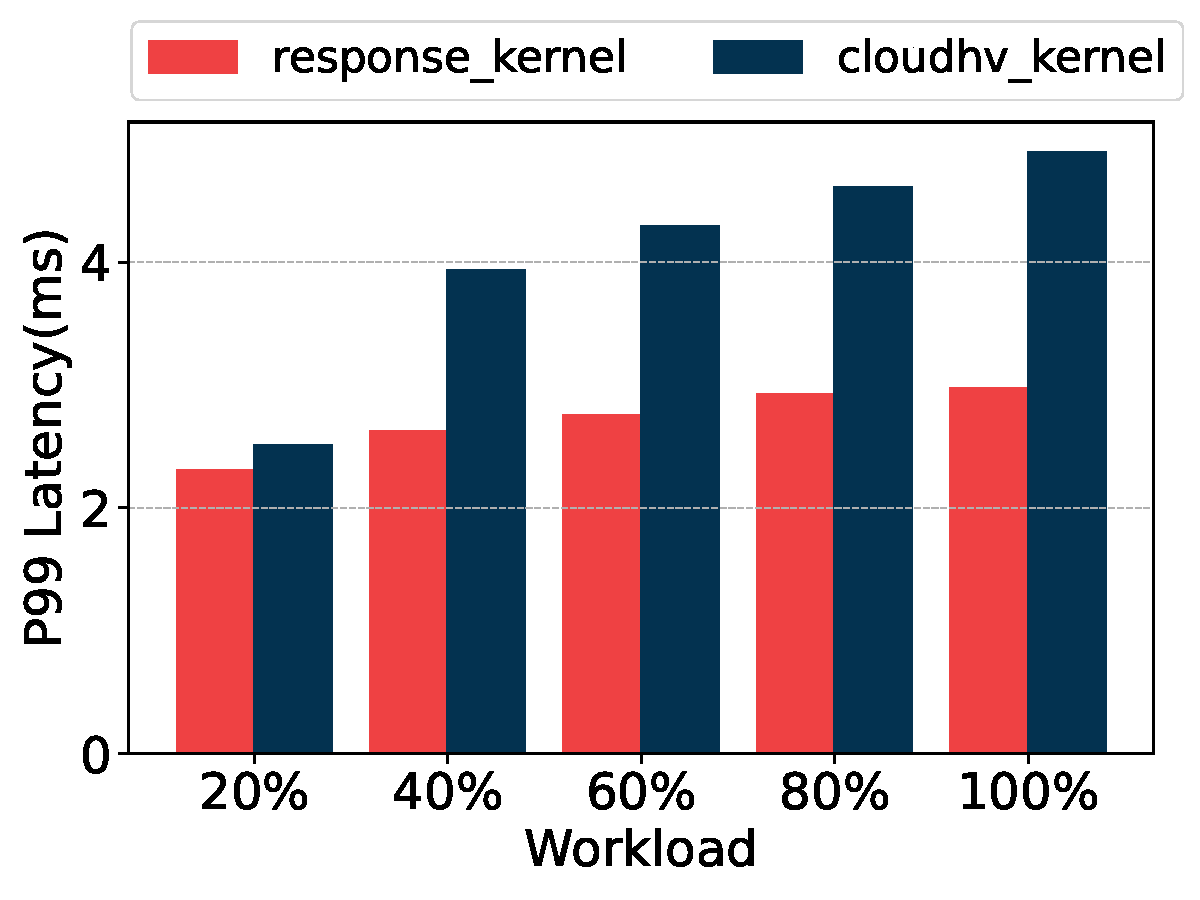
\includegraphics[width=\textwidth]{response_kernel_redis}
      \caption{Redis请求延迟}
      \label{fig:response_kernel_redis}
    \end{subfigure}
    \begin{subfigure}[b]{0.32\textwidth}
      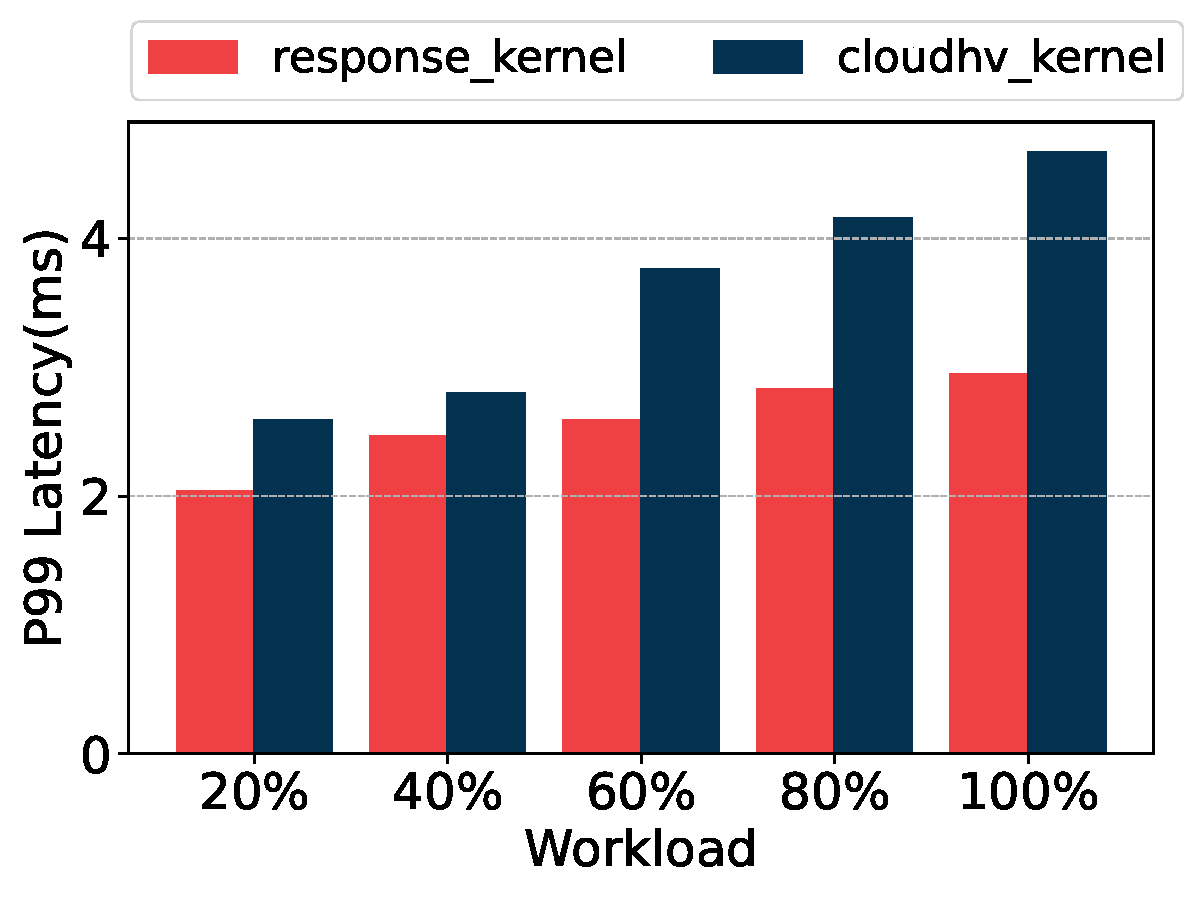
\includegraphics[width=\textwidth]{response_kernel_memcached}
      \caption{Memcached请求延迟}
      \label{fig:response_kernel_memcached}
    \end{subfigure}
    \begin{subfigure}[b]{0.32\textwidth}
        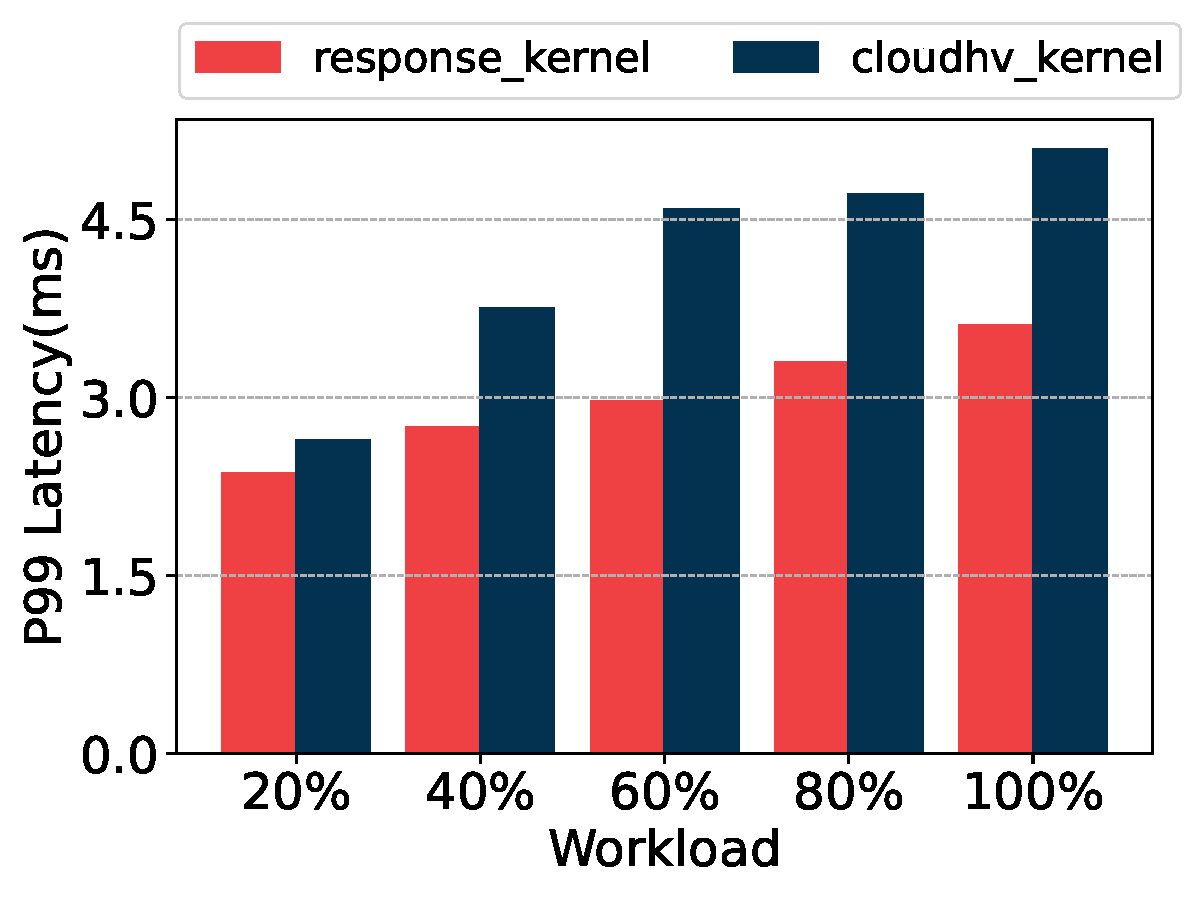
\includegraphics[width=\textwidth]{response_kernel_nginx}
        \caption{Nginx请求延迟}
        \label{fig:memcached_response}
      \end{subfigure}
      \begin{subfigure}[b]{0.32\textwidth}
        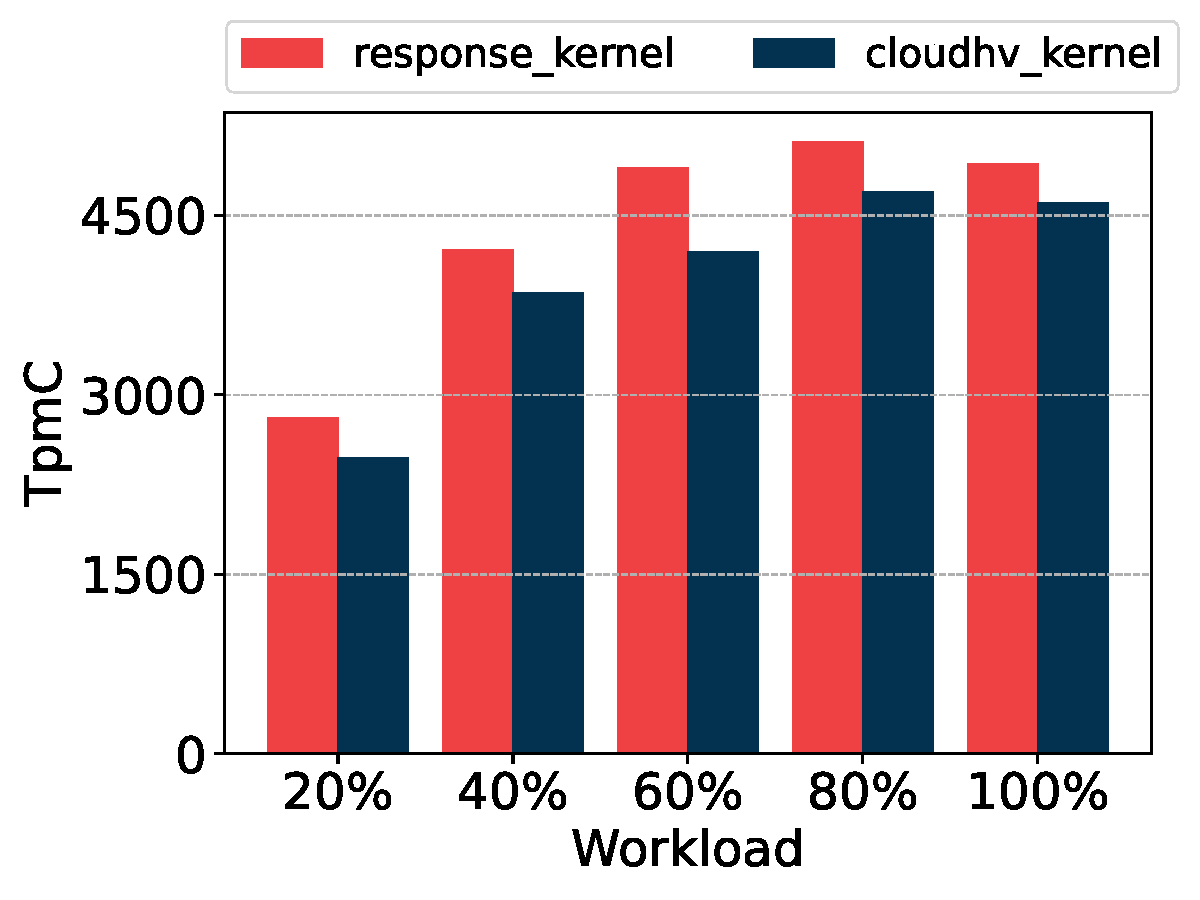
\includegraphics[width=\textwidth]{response_kernel_mysql}
        \caption{\quad MySQL每秒事务数量}
        \label{fig:memcached_response}
      \end{subfigure}
      \begin{subfigure}[b]{0.32\textwidth}
        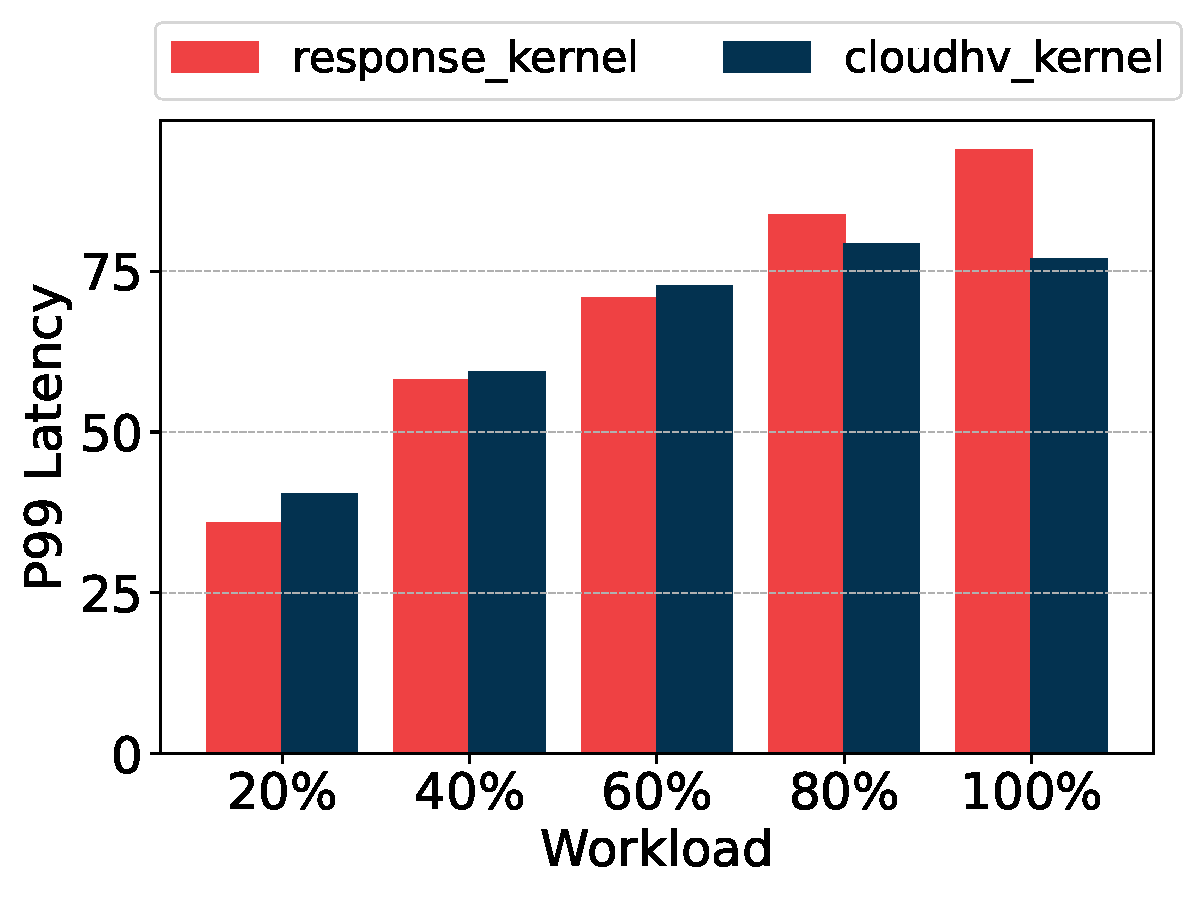
\includegraphics[width=\textwidth]{response_kernel_mysql_latency}
        \caption{MySQL请求延迟}
        \label{fig:memcached_response}
      \end{subfigure}
    \bicaption{\quad 响应度优先内核在LC混部场景下的效果}{\quad The effect of response-first kernel in LC Co-Location scenario}
    \label{fig:perf_response}
\end{figure}

\subsection{吞吐量优先内核性能}

% graph500(time) \ ffmjpeg 

吞吐量优先任务调度配置使用HZ\_100配置时钟中断,并开启PREEMPT\_NONE抢占模式。实验在4 CPU、1024MB内存的虚拟机上展开,选择Graph500、ffmjepg两种CPU敏感型应用分别与stress\_ng CPU干扰应用混部,并与使用HZ\_250和VOLUNTARY抢占模式的CloudHypervisor默认Linux内核进行比较。Graph500主要执行图计算算法,因此执行时间是其重要的性能指标,实验中使用time工具记录进程在用户态与内核态耗费的时间,并将平均每分钟能够执行的Graph500计算数量作为性能指标。FFmjpeg是主流的媒体处理工具,实验中使用vBench模拟负载并同样记录进程在用户态与内核态耗费的时间,而对于媒体处理应用而言,每秒处理帧数是其重要的性能指标。

\begin{figure}[H]
    \centering
    \begin{subfigure}[b]{0.35\textwidth}
        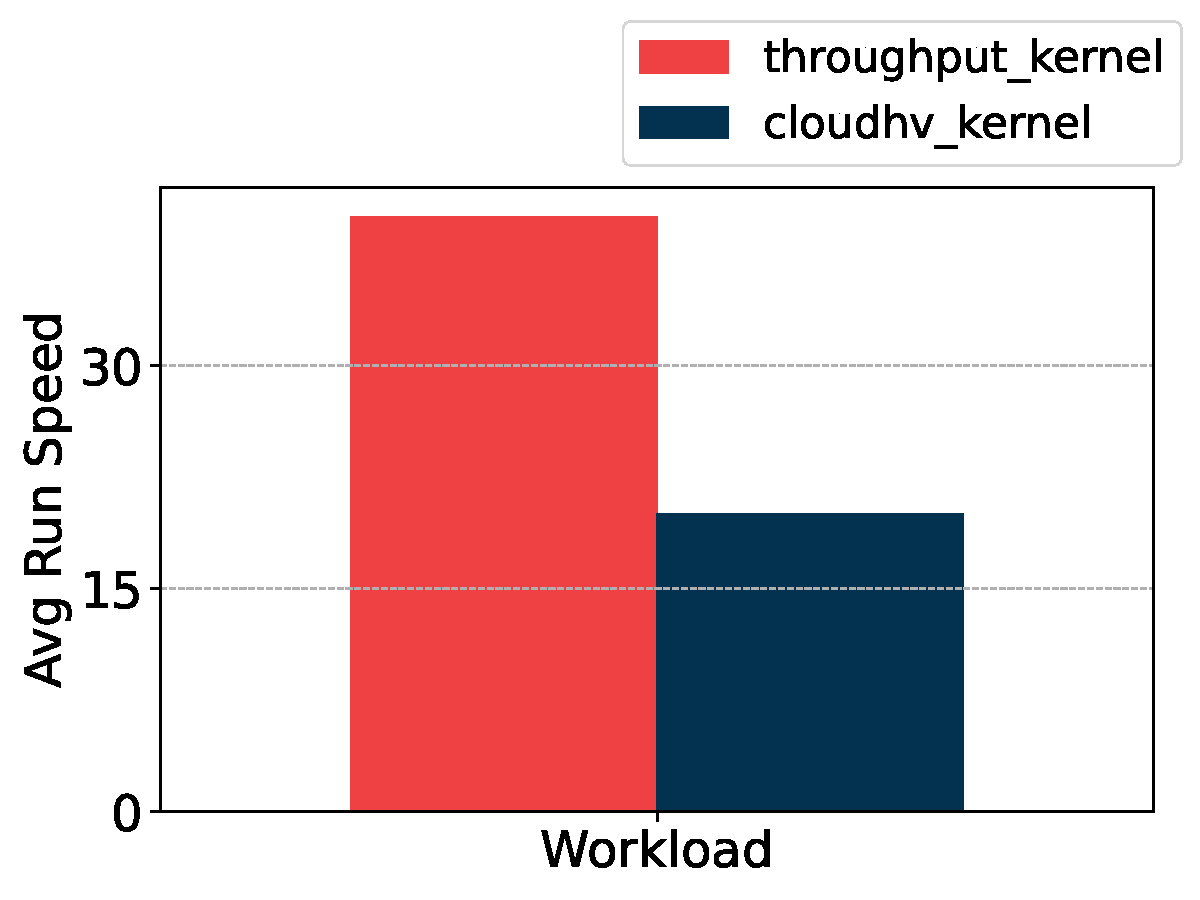
\includegraphics[width=\textwidth]{throughput_kernel_graph500_speed}
        \caption{\quad Graph500每分钟执行数量}
        \label{fig:throughput_kernel_graph500_speed}
    \end{subfigure}
    \begin{subfigure}[b]{0.35\textwidth}
        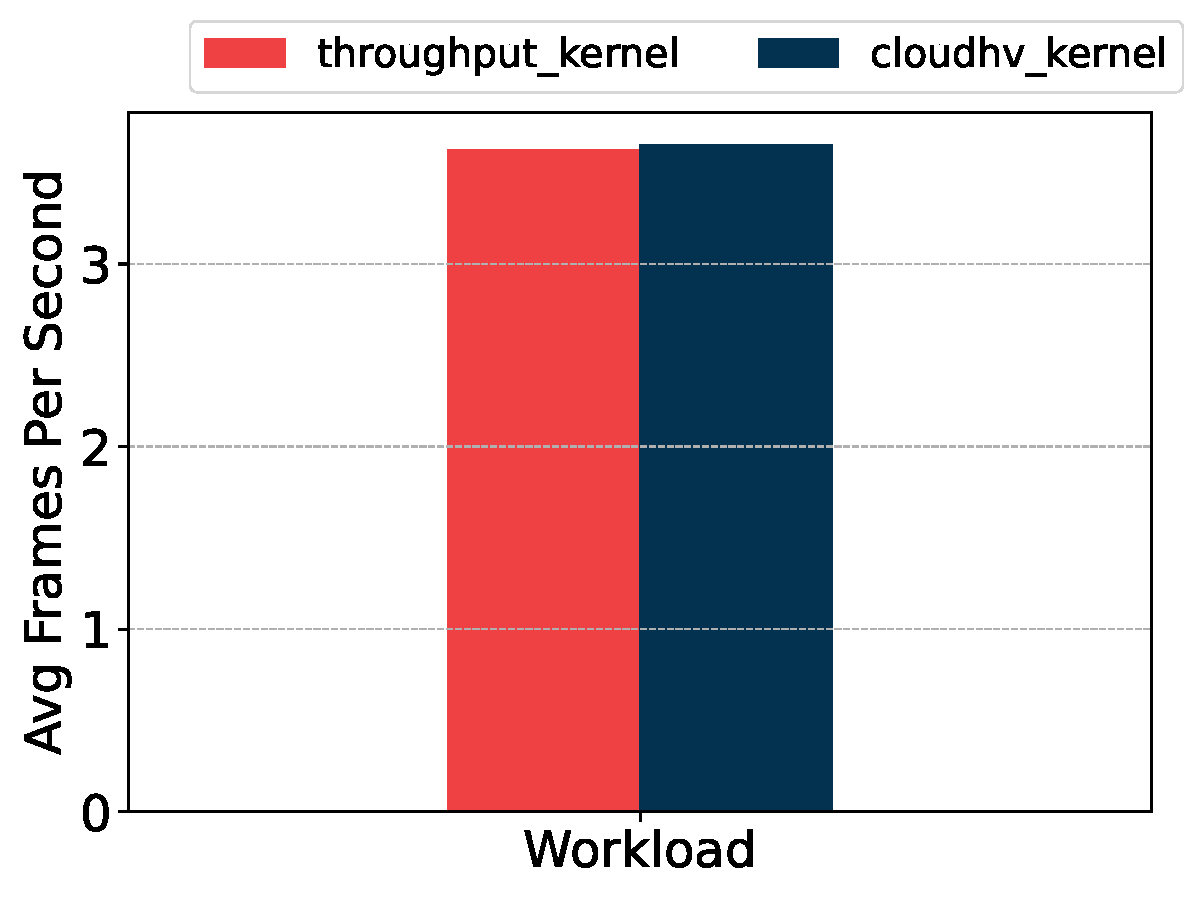
\includegraphics[width=\textwidth]{throughput_kernel_ffmpeg_speed}
        \caption{\quad FFmpeg每秒处理帧数量}
        \label{fig:throughput_kernel_ffmpeg_speed}
    \end{subfigure}
    \bicaption{\quad 吞吐量优先内核在BE混部场景下的效果}{\quad The effect of throughput-first kernel in BE Co-Location scenario}
    \label{fig:perf_throughput}
\end{figure}

混部实验结果如图~\ref{fig:perf_throughput}所示。对于Graph500,吞吐量优先内核实现了平均执行速度提升165.2\%的效果。而在如图~\ref{fig:perf_throughput_time}所示的运行时间分布上可以看出,Graph500在吞吐量优先内核下,得益于保守的抢占模式与较低的时钟中断频率,使得在内核态运行的时间大大减少。同时,更少的上下文切换也提升了应用执行的局部性,使得Graph500在用户态的运行时间也有所减少。而对于FFmjpeg,吞吐量优先内核与CloudHV默认内核的差异并不明显。这是因为不同于Graph500,FFmjpeg在运行过程中需要频繁进行IO来读取媒体文件,因此等待IO的时间更多,此时即便设置更小的时钟中断频率,但对于提升应用性能上意义并不大。

\begin{figure}[H]
    \centering
    \begin{subfigure}[b]{0.35\textwidth}
        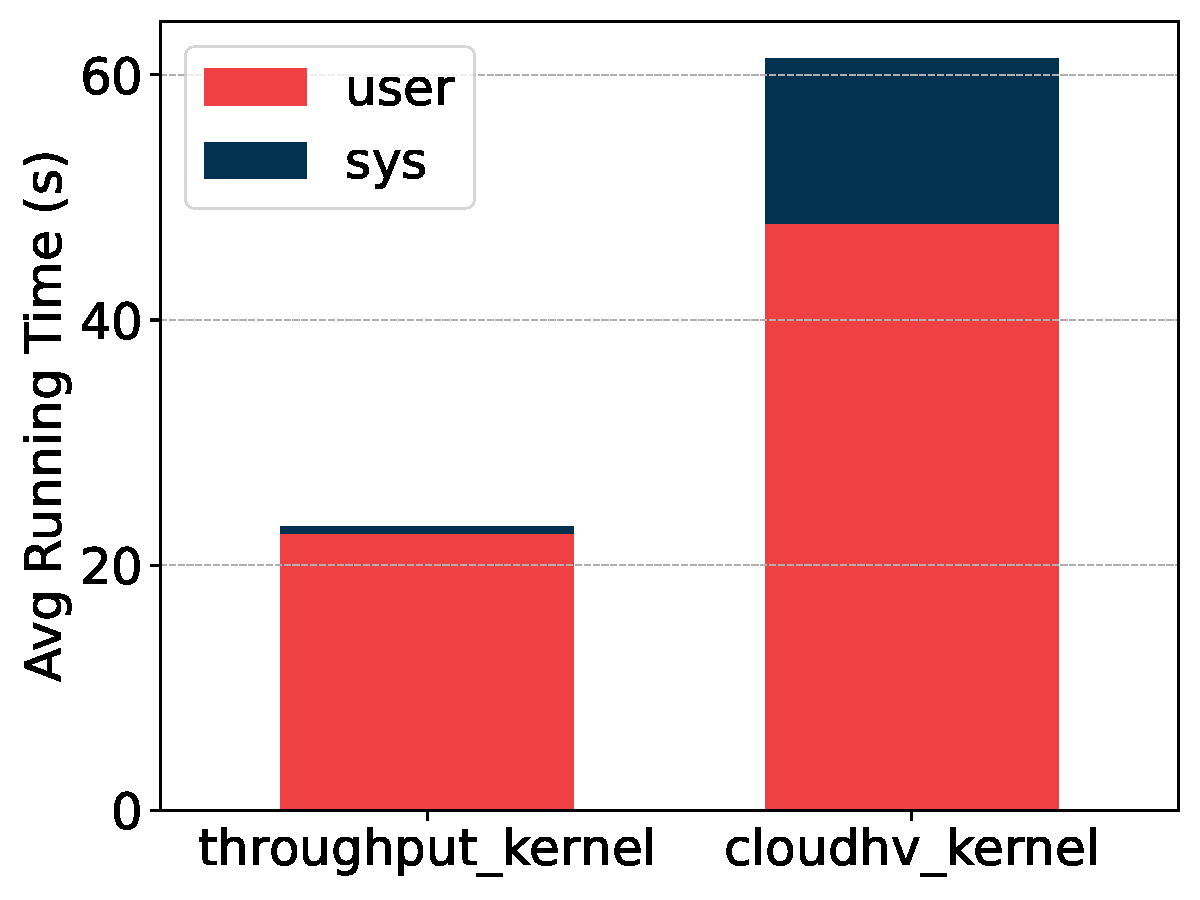
\includegraphics[width=\textwidth]{throughput_kernel_graph500}
        \caption{\quad Graph500平均运行时间分布}
        \label{fig:throughput_kernel_graph500}
    \end{subfigure}
    \begin{subfigure}[b]{0.35\textwidth}
        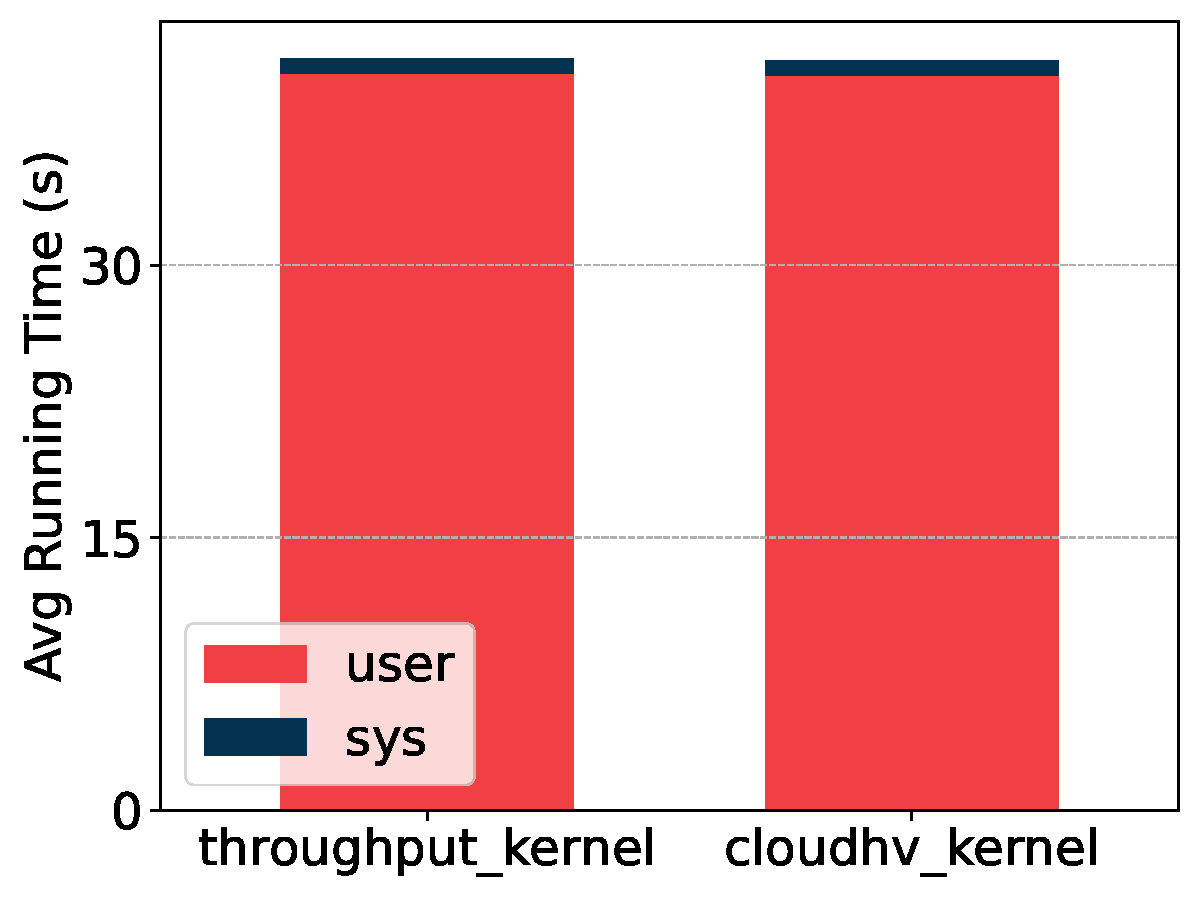
\includegraphics[width=\textwidth]{throughput_kernel_ffmpeg}
        \caption{\quad FFmpeg平均运行时间分布}
        \label{fig:throughput_kernel_ffmpeg}
    \end{subfigure}
    \bicaption{\quad 混部场景下BE应用时间分布}{\quad BE application time distribution in Co-Location scenario}
    \label{fig:perf_throughput_time}
\end{figure}

\subsection{CPU资源感知策略效果}

% 普通场景
% 硬件场景:SMT

Control Tower CPU感知调度策略首先验证调度策略对高优先级任务的QoS保障能力,实验在4 CPU、1024 MB内存的虚拟机中展开,选择Redis、Memcached、Nginx与MySQL作为高优先应用来与stress\_ng CPU干扰混部,内核采用与CloudHV默认内核相同的HZ与抢占模式,并与CloudHV默认内核进行比较。

混部结果如图~\ref{fig:lc_bpf_sched}所示,总体来看,CPU资源感知调度策略几乎总是能够让LC应用达到与未受干扰情况下相近的性能。对于常见的LC应用Redis、Memcached与Nginx,CPU资源感知调度策略分别实现降低99分位尾延迟最高90.4\%、61.1\%、63.3\%的效果,同时在各个负载强度下均能有效保障应用的QoS。而对于业务逻辑较复杂的MySQL,CPU资源感知调度策略也同样能够很好地进行QoS保障,如图~\ref{fig:bpf_sched_smp_mysql}所示,在MySQL不同负载强度中,CPU感知调度策略实现了MySQL平均事务处理数量提升最高60.8\%的效果,同时请求延迟也最高降低了68.3\%。

\begin{figure}[H]
    \centering
    \begin{subfigure}[b]{0.32\textwidth}
        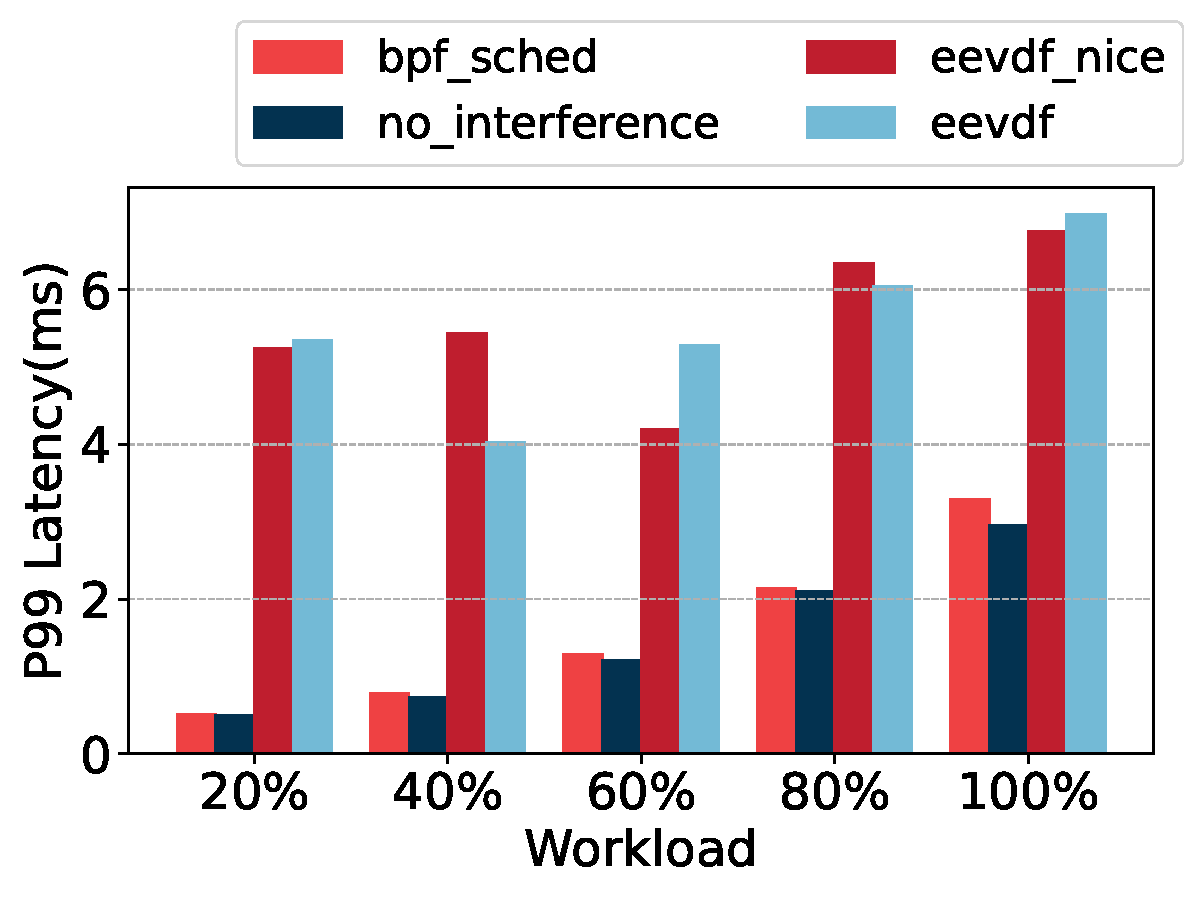
\includegraphics[width=\textwidth]{bpf_sched_smp_redis}
        \caption{\quad Redis请求延迟}
        \label{fig:bpf_sched_smp_memcached}
    \end{subfigure}
    \begin{subfigure}[b]{0.32\textwidth}
        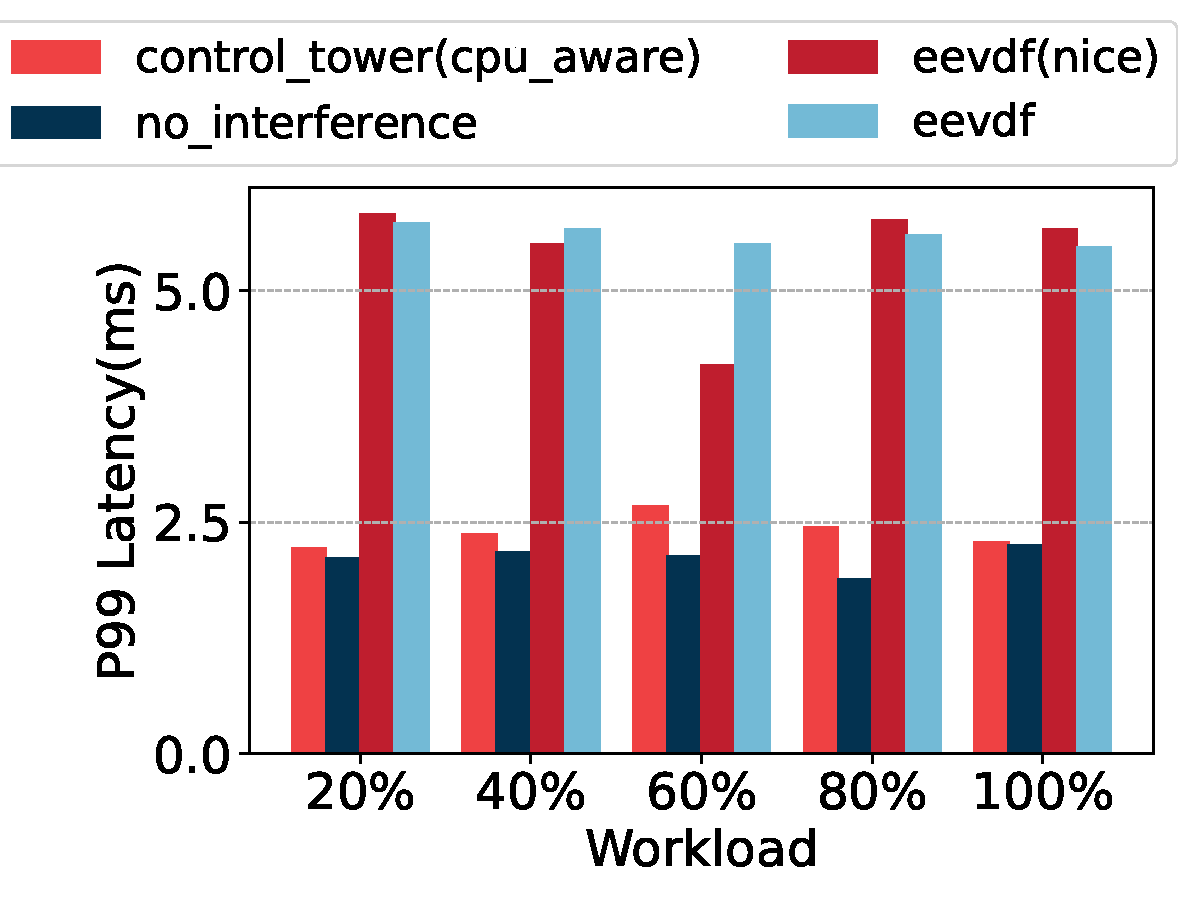
\includegraphics[width=\textwidth]{bpf_sched_smp_memcached}
        \caption{\quad Memcached请求延迟}
        \label{fig:bpf_sched_smp_memcached}
    \end{subfigure}
    \begin{subfigure}[b]{0.32\textwidth}
        \includegraphics[width=\textwidth]{bpf_sched_smp_nginx}
        \caption{\quad Nginx请求延迟}
        \label{fig:bpf_sched_smp_memcached}
    \end{subfigure}
    \begin{subfigure}[b]{0.32\textwidth}
        \includegraphics[width=\textwidth]{bpf_sched_smp_mysql}
        \caption{\quad MySQL每秒事务数量}
        \label{fig:bpf_sched_smp_mysql}
    \end{subfigure}
    \begin{subfigure}[b]{0.32\textwidth}
        \includegraphics[width=\textwidth]{bpf_sched_smp_mysql_latency}
        \caption{\quad MySQL请求延迟} 
        \label{fig:bpf_sched_smp_mysql_latency}
    \end{subfigure}

\bicaption{\quad 混部场景下CPU感知调度下的LC应用QoS保障效果}{\quad LC Application Latency Stability}
\label{fig:lc_bpf_sched}
\end{figure}

在总体吞吐上,不同调度算法下的系统CPU总体利用率如图~\ref{fig:cpu_usage}所示。其中,对于Redis、Memcached、Nginx而言,混部场景中总体CPU资源使用率几乎都完全占满。对比无干扰下的CPU资源使用率,能够发现额外的CPU资源占用由干扰应用产生,此时分配CPU资源的方式决定了混部场景下QoS保障的效果。

\begin{figure}[H]
    \centering
    \begin{subfigure}[b]{0.33\textwidth}
        \includegraphics[width=\textwidth]{cpu_usage_redis}
        \caption{Redis-干扰}
        \label{fig:cpu_usage_redis}
    \end{subfigure}
    \begin{subfigure}[b]{0.33\textwidth}
        \includegraphics[width=\textwidth]{cpu_usage_memcached}
        \caption{Memcached-干扰}
        \label{fig:cpu_usage_memcached}
    \end{subfigure}
    \begin{subfigure}[b]{0.33\textwidth}
        \includegraphics[width=\textwidth]{cpu_usage_mysql}
        \caption{MySQL-干扰}
        \label{fig:cpu_usage_mysql}
    \end{subfigure}
    \begin{subfigure}[b]{0.33\textwidth}
        \includegraphics[width=\textwidth]{cpu_usage_nginx}
        \caption{Nginx-干扰}
        \label{fig:cpu_usage_nginx}
    \end{subfigure}
\bicaption{\quad 混部场景CPU总使用率}{\quad Total CPU usage in co-location scenarios}
\label{fig:cpu_usage}
\end{figure}

相较于Linux任务调度机制,CPU感知调度策略能够做到更好的QoS保障效果,核心原因在于合理地CPU资源分配。CPU感知调度策略基于Control Tower任务调度框架设计,使得低优先任务总是能够在高优先应用需要时及时地出让CPU资源,并在高优先应用运行的过程中确保不进行抢占,从而实现更好的QoS保障效果。

混部场景中调度需要考虑硬件的特性,如SMT中兄弟核心之间存在片上共享资源,Linux任务调度策略中的措施是通过调度域名尽量避免将任务调度到SMT上,但这种做法并不能充分利用SMT资源。造成上述问题的核心在于缺少一种CPU感知的机制,让SMT调度时知道兄弟核心的运行情况,而CPU感知调度策略恰好能够解决这一问题。

混部实验在2 SMT CPU、1024 MB内存的虚拟机中展开,选择Redis、Memcached、Nginx、MySQL四种延时敏感应用与stress\_ng CPU干扰进行混部。实验结果如图~\ref{fig:lc_bpf_sched_smt}所示,相较于EEVDF,CPU感知调度策略能够在所测应用的各个负载下有效地对应用QoS进行保障。其中对于Redis、Memcached、MySQL,CPU感知调度策略分别实现了99分位尾延迟降低最高71.2\%、48.7\%、49.5\%的效果。特别地,Nginx在高负载时由于SMT场景的激烈资源竞争,Linux EEVDF调度器几乎无法进行有效调度,导致Nginx延时呈数量级的上升,而在该场景下,如图~\ref{fig:bpf_sched_smt_nginx}所示,CPU感知调度策略则仍然能够实现Nginx与无干扰类似的性能表现。

\begin{figure}[H]
    \centering
    \begin{subfigure}[b]{0.32\textwidth}
        \includegraphics[width=\textwidth]{bpf_sched_smt_redis}
        \caption{\quad Redis请求延迟}
        \label{fig:bpf_sched_smt_redis}
    \end{subfigure}
    \begin{subfigure}[b]{0.32\textwidth}
        \includegraphics[width=\textwidth]{bpf_sched_smt_memcached}
        \caption{\quad Memcached请求延迟}
        \label{fig:bpf_sched_smt_memcached}
    \end{subfigure}
    \begin{subfigure}[b]{0.32\textwidth}
        \includegraphics[width=\textwidth]{bpf_sched_smt_nginx}
        \caption{\quad Nginx请求延迟}
        \label{fig:bpf_sched_smt_nginx}
    \end{subfigure}
    \begin{subfigure}[b]{0.32\textwidth}
        \includegraphics[width=\textwidth]{bpf_sched_smt_mysql}
        \caption{\quad MySQL每秒事务数量}
        \label{fig:bpf_sched_smt_mysql}
    \end{subfigure}
    \begin{subfigure}[b]{0.32\textwidth}
        \includegraphics[width=\textwidth]{bpf_sched_smt_mysql_latency}
        \caption{\quad MySQL请求延迟}
        \label{fig:bpf_sched_smt_mysql_latency}
    \end{subfigure}
\bicaption{\quad SMT混部场景下,CPU感知调度下的LC应用QoS保障}{\quad LC Application Latency Stability}
\label{fig:lc_bpf_sched_smt}
\end{figure}

Control Tower CPU感知调度策略在保障延时的同时,同时也保障了延时的稳定度,这点对于LC应用而言也十分重要。以Redis为例,如图~\ref{fig:latency_box}所示,在CPU感知调度策略下,Redis的各个负载下的延时波动都几乎与无干扰状态下相同。

\begin{figure}[H]
    \centering
    \begin{subfigure}[b]{0.35\textwidth}
        \includegraphics[width=\textwidth]{cpu_aware_box_no_interference}
        \caption{无干扰场景}
        \label{fig:cpu_aware_box_no_interference}
    \end{subfigure}
    \begin{subfigure}[b]{0.35\textwidth}
        \includegraphics[width=\textwidth]{cpu_aware_box_bpf_sched}
        \caption{CPU感知调度策略}
        \label{fig:cpu_aware_box_bpf_sched}
    \end{subfigure}
    \begin{subfigure}[b]{0.35\textwidth}
        \includegraphics[width=\textwidth]{cpu_aware_box_eevdf}
        \caption{EEVDF调度器}
        \label{fig:cpu_aware_box_eevdf}
    \end{subfigure}
    \begin{subfigure}[b]{0.35\textwidth}
        \includegraphics[width=\textwidth]{cpu_aware_box_eevdf_nice}
        \caption{EEVDF高优先级}
        \label{fig:cpu_aware_box_eevdf_nice}
    \end{subfigure}
\bicaption{\quad Redis延迟稳定性}{\quad LC Application Latency Stability}
\label{fig:latency_box}
\end{figure}

实现这一延时保障效果的核心原因在于Control Tower任务调度框架中的eBPF数据源与BPF调度策略都完全运行在内核态,并借助内核提供的数据结构交互,因此在调度决策上速度上能够做到与内核调度周期同步,从而避免了许多用户态调度器存在的“乒乓效应”。

\subsection{网络资源感知策略效果}

Control Tower网络资源感知调度策略实验在一个4CPU、1024MB内存的虚拟机展开。首先,截取Redis、Memcached、Nginx与Mysql四个常见网络服务型应用在一段时间内的负载与epoll时间计数。如图~\ref{fig:epoll_request}所示,对于Redis、Memcached、Nginx三种应用而言,epoll wait返回的事件数量与请求量高度相关,而考虑epoll事件的统计发生在服务端,而请求数量的统计发生在客户端,因此两端序列在时间上存在一定的偏移。然而,对于没有使用epoll作为底层网络机制实现的MySQL,这种监测方式就不能反映应用的网络资源使用,需要依赖其他的手段。由此也反映出,在不同的混部场景下对监测手段的要求也不同。

\begin{figure}[!htbp]
    \centering
    \begin{subfigure}[b]{0.49\textwidth}
        \includegraphics[width=\textwidth]{epoll_memcached}
        \caption{Memcached请求数量与Epoll Wait事件数量}
        \label{fig:epoll_memcached}
    \end{subfigure}
    \begin{subfigure}[b]{0.49\textwidth}
        \includegraphics[width=\textwidth]{epoll_redis}
        \caption{Redis请求数量与Epoll Wait事件数量}
        \label{fig:epoll_redis}
    \end{subfigure}
    \begin{subfigure}[b]{0.49\textwidth}
        \includegraphics[width=\textwidth]{epoll_nginx}
        \caption{Nginx请求数量与Epoll Wait事件数量}
        \label{fig:epoll_nginx}
    \end{subfigure}
    \begin{subfigure}[b]{0.49\textwidth}
        \includegraphics[width=\textwidth]{epoll_mysql}
        \caption{Mysql请求数量与Epoll Wait事件数量}
        \label{fig:epoll_mysql}
    \end{subfigure}
\bicaption{\quad LC应用负载与Epoll事件}{\quad Requests and Epoll Events on LC}
\label{fig:epoll_request}
\end{figure}

网络资源感知策略下的混部实验选择Nginx作为LC应用,并将其最大负载的20\%作为调度的临界值。混部结果如图~\ref{fig:network_aware_cpu_usage}所示,其中红色虚线部分标注了调度策略的负载临界值。时序图中,Nginx负载不断增加,同时CPU占用率也有所上升,在临界值之前,由于调度策略较宽松,整体调度以吞吐量为目标,因此系统总CPU利用率接近100\%,而随负载的不断增加,应用间CPU资源争抢越来越激烈,整体CPU资源波动较大。临界值之后,调度策略转变为以保障LC应用延时为目标,并开始严格限制低优先任务的CPU资源使用。此时虽然整体CPU利用率随Nginx负载增大而有所降低,但整体CPU利用率波动变得更小,同时也保障了Nginx的QoS。

\begin{figure}[H]
    \centering
    \includegraphics[width=0.9\textwidth]{network_aware_cpu_usage}
    \bicaption{\quad Nginx混部场景CPU利用率}{\quad CPU utilization in mixed deployment scenario of Nginx}
    \label{fig:network_aware_cpu_usage}
\end{figure}

% \subsection{内存资源感知策略}
% Redis

\section{本章小结}

本章主要首先针对画像分析中不同类型应用,基于内核中关于HZ与抢占模型的配置,设计了调度配置的定制优化,提供了吞吐量优先与响应度优先两种不同调度目标的内核配置。

随后,为解决混部场景下,Linux任务调度机制调节手段单一、优先性存在缺陷的问题,设计实现了Control Tower任务调度框架。框架基于Sched Ext项目实现,首先,框架允许通过用户输入与eBPF插桩,为调度策略提供丰富的决策信息。其次,框架借助Ext调度类的优先级特点,实现任务的全局高优先性。最后,框架利用BPF调度策略的灵活性,能够针对不同的混部场景,定制混部任务所需的调度方式。

在Control Tower任务调度框架的基础上,本文进一步设计了CPU感知的任务调度策略与网络资源感知的任务调度策略。其中,CPU感知任务调度策略通过感知高优先任务的CPU资源使用情况,结合用户定义的CPU阈值,在利用系统中的空闲CPU资源的同时,也能结合混部场景中CPU资源的不同特性来快速地向高优先任务出让CPU资源,从而实现有效的QoS保障。网络资源感知调度策略则通过监听epoll\_wait系统调用,了解系统中网络应用的负载情况,并适时地调整调度策略,以便于在网络应用的不同负载下进行区别性地管理。

本章实验中,首先围绕内核任务调度配置在虚拟化环境中展开实验。其中,响应度优先内核能够在混部场景下,能够最高降低LC应用39.2\%的延迟。吞吐量优先内核则能够在混部场景下,最高提升应用165.2\%的执行速度。随后,在Control Tower任务调度框架的实验中,CPU感知调度策略能够在混部实验中,相较于Linux任务调度实现90.4\%的延迟降低效果,并在混部任务的的各个负载下,是其接近于单独部署时的性能。除此之外,CPU感知调度策略也能够很好的解决SMT混部场景下的调度问题。
\chapter{运行时可定制调度的沙箱机制实现}\label{chap:control_zone}

\section{概述}

数据中心混合部署对调度提出了两大挑战。首先,在硬件上,现代服务器上拥有丰富的计算资源,能够支持大量的任务同时运行,同时硬件环境也相对复杂,因此调度需要充分考虑硬件的特性,从而避免如"吵闹邻居"等情况出现。其次,在软件上,数据中心运行的应用种类十分丰富,而通常依据应用对延迟的敏感性分为LC与BE两大类,前者要求调度足够迅速,从而满足交互式应用对响应度的要求,后者则希望长时间的运行,要求调度不能过于频繁,从而满足吞吐量的需求。

而根据第三章中的画像分析,不同应用各种资源的需求也有所不同,对于有相同资源需求的应用,混部时依赖隔离手段来避免关键资源上的竞争,而对于有不同资源需求的应用,可以进行混部来提升资源使用率,但同时也依赖调度机制来及时地保障高优先级应用的QoS。

\section{Control Zone设计}

% 概述 -> 设计思路

% 介绍 Control Zone 的概念
% - 面对什么场景
% - 存在哪些问题
%   - 复杂的硬件环境
%   - 复杂的软件环境
% - 针对每个问题的解决方式
% - 设计目标

本研究提出了Control Zone,一种面向混部的沙箱系统。在航空领域,Control Zone指受控空域的一部分,通常在机场的周围,保护进出机场的的空中交通,而在Control Zone之中,由塔台进行飞机的调度。本研究借用Control Zone概念设计沙箱系统,在外层提供足够强的隔离性,而在内层则提供运行时可定制的调度器,Control Zone包含如下特性:

1)轻量级虚拟机:Control Zone使用虚拟机来提供更强的隔离性,而轻量化体现在两方面,一方面采用轻量化的Hypervisor,提供更快的虚拟机启动速度与内存占用, 另一方使用最小化Guest内核及精简根文件系统,提供快速的系统引导与基本的系统功能。

2)运行容器化的任务:Control Zone包含一个最小化的容器环境与容器运行时,支持大量容器化应用的运行,同时享容器镜像与目录文件能够在不同的Control Zone之间共享,支持跨Control Zone的任务协作。

3)可定制的调度器:Control Zone支持Sched Ext可扩展调度类,能够运行BPF Scheduler。Control Zone提供基础的BPF Scheduler容器镜像模板,并提供了集中基础的BPF Scheduler容器,使得调度器能够与任务一样一起进行管理,并支持运行时热切换。

4)可观测基础设施:沙箱系统包含了一个围绕虚拟机的可观测性系统,能够从Host、Hypervisor、App三个层次以虚拟机为粒度采集丰富的指标,并提供实时监测与离线分析功能来全面地分析虚拟机及其中任务的性能。

\begin{figure}[!htbp]
    \centering
    \includegraphics[width=1.0\textwidth]{controlzone_arch}
    \bicaption{\quad Control Zone基本架构}{\quad Control Zone Architectural}
    \label{fig:controlzone_arch}
\end{figure}
 
运行时可定制调度的沙箱机制通过如图~\ref{fig:controlzone_arch}所示,管理器负责进行Control Zone的管理,提供隔离环境的定制能力,并可以根据混部任务的属性动态地对BPF Scheduler进行修改,可观测性基础设置则能够与各层次的系统组件交互,以采集全面的虚拟机指标信息。

对于硬件上的挑战,首先,参考Linux中调度域的划分,可以对Control Zone的硬件资源特征标注,运行在不同Control Zone中的任务可以借助Control Zone的隔离能力,最大程度并发运行并避免相互干扰,而在Control Zone之中,则可以根据硬件资源特征匹配合适的内核与BPF调度器,针对性地处理硬件存在的调度问题。

对于软件上的挑战,首先,对于不同类型的单个任务,可以匹配合适的Guest内核来满足响应度或吞吐量上的需求。而对于混部任务,可以选择合适的内核调度策略、BPF调度策略或自定义BPF调度策略,来满足优先级保障,同时借助可观测性基础设施提供的持续监测能力,在运行过程中发现Control Zone的性能问题,随后,一方面能够通过修改外层的资源隔离配置,为Control Zone分配更多的资源,另一方面也可以动态修改Control Zone之中的BPF调度策略,来保障高优先级任务的性能。

\section{Control Zone实现}

\subsection{Control Zone组成}

% 优化图例
% 使用中文名称,体现功能
% Control Zone组成,阐述各个组成部分所做的功能,希望实现的目标
% - czctrl: Control Zone管理
% - czdaemon: 容器管理
%   - chsd: 调度策略管理
% - observity: 可观测性

运行时可定制调度的沙箱包括Control Zone管理、应用管理及可观测性三个主要部分。如图~\ref{fig:cz_components}所示,用户通过czyaml配置文件来定义一个Control Zone,而Control Zone的管理主要czctrl、czmanager及虚拟化运行时三个组件协作完成。每个Control Zone都运行有一个czdaemon,并与czctrl、czmanager协作实现应用管理。可观测性沿用了第三章中设计的在线指标监测系统,通过与czmanager的协作完成对于虚拟机的监控。镜像存储服务负责管理OCI镜像,并在Control Zone管理的各个阶段提供镜像存储服务。

\begin{figure}[!htbp]
    \centering
    \includegraphics[width=0.9\textwidth]{cz_components}
    \bicaption{\quad Control Zone组件结构}{\quad Components of Control Zone}
    \label{fig:cz_components}
\end{figure}

1)czyaml:Control Zone定义。czyaml包含Meta、Guest、Resource三部分,其中Meta包含一些元数据,用以区分不同的Control Zone。Guest部分则用于声明运行环境,包括使用的系统、调度器及根文件系统。Resource部分用于声明隔离的资源,包括常见的CPU、Memory以及Intel RDT子系统中的LLC和内存带宽。

2)czmanager:Control Zone管理。czmanager负责Control Zone的实际管理, 包括创建、查看、启动、暂停、更新以及清除等完善的生命周期管理。过程中czmanager主要负责维护Control Zone的状态,并协同底层虚拟化运行时实现最终的虚拟机管理。而在可观测性上,czmanager利用了虚拟机各层次的信息生成监控配置,并与可观测性基础设施协作以实现Control Zone的持续监控。资源管理上,czmanager主要与虚拟化运行时、Linux Resctrl及Cgroup子系统交互,根据czyaml中的定义实现Control Zone的资源隔离。

3)czdaemon:Control Zone守护程序。czdaemon运行在每个Control Zone之中,在启动阶段主要用来信息获取与状态探测。而在启动完成之后,作为Control Zone内外沟通的桥梁,对外与czmanager交互,以接收命令,对内则直接与容器运行时交互,实现镜像及容器的管理。

4)czctrl:用户命令行工具。czctrl是所有请求的入口,能够解析用户输入的命令并验证czyaml配置,随后再与czmanager交互以达成用户管理Control Zone和任务的目的。

5)镜像存储服务:容器及其他静态资源管理。应用与BPF Scheduler都以OCI容器镜像的形式保存在镜像存储服务中,并通过容器的形式运行,同时为方便其他静态资源的管理,预编译内核及根文件系统也保存在精简容器镜像的中交给镜像存储服务管理。

\subsection{Control Zone流程}

% 要解决的问题,以及解决的问题的思路

% Control Zone Yaml
% Control Zone关键流程的执行过程
% - start
% - stop 
% - update
% - remove
% Control Zone容器的管理流程
% - add
% - delete
% Control Zone调度的流程
% - czctrl的资源限制
% - chsd的策略控制
% - sched ext的策略控制

Control Zone Yaml提供了丰富的资源隔离配置~\ref{tab:cz_config},隔离性围绕三个层次进行设计,首先,虚拟机本质上是一种特殊的进程,Linux中提供了Cgroup技术来隔离进程的资源,因此在配置文件中,允许声明Cgroup配置参数,来限制如虚拟机能够使用的CPU核心等,同时作为进程,也能够被Linux Resctrl子系统管理,从而构造LLC与内存带宽的隔离。其次,虚拟机本身还由Hypervisor管理,而大部分Hypervisor都提供了额外的资源隔离机制,主要体现在硬件模拟上,如对于CPU,可以限制提供给虚拟机使用的CPU feature,而对于其他设备,则提供了对virtio net设备的收发速度及virtio blk设备的读写速度的控制。最后,虚拟机内的guest os本身也能够提供一些隔离机制,在Control Zone中能够通过调度子系统来对不同的任务进行隔离,如将任务划分到不同优先级的调度队列中, 从而在相同调度队列上构造任务粒度的隔离性,这一配置通常与混部任务一同设置。

\begin{table}
    \bicaption{\quad Control Zone配置列表}{\quad Control Zone Config}% caption
    \label{tab:cz_config}
    \footnotesize% fontsize
    \setlength{\tabcolsep}{4pt}% column separation
    \renewcommand{\arraystretch}{1.5}% row space 
    \centering
    \begin{tabular}{lcc}
        \hline
        %\multicolumn{num_of_cols_to_merge}{alignment}{contents} \\
        %\cline{i-j}% partial hline from column i to column j
        类型 & 配置 & 说明\\
        \hline
        Meta & name & Control Zone名称 \\
        & workdir & Control Zone工作目录,存放日志及其他配置 \\
        & share\_folder(可选) & 额外共享给Control Zone的目录 \\
        & label & 标签,数个key-value对 \\
        & vrun & 虚拟机运行时,可选CloudHypervisor、Qemu或Libvirtd \\
        Guest & kernel(可选) & Control Zone使用的内核,从镜像存储拉取 \\
        & initramfs(可选) & 初始化内存文件系统,默认情况下不使用 \\
        & rootfs(可选) & Control Zone使用的根文件系统,从镜像存储拉取\\
        & kcmdline(可选) & 内核的运行命令 \\
        Resource & [cgroup] & 虚拟机Cgroup配置 \\
        & cpu.max & 最大CPU使用限制 \\
        & cpu.max.burst & 最大突发CPU使用限制 \\
        & cpuset.cpus & CPU亲和性 \\
        & cpuset.mems & 内存节点亲和性 \\
        & [hypervisor] & 虚拟机hypervisor配置 \\
        & cpu features& vCPU可用的特性\\
        & bw\_size & 设备带宽大小(byte/s)\\
        & bw\_one\_time\_burst & 设备突发带宽大小(byte/s)\\
        & bw\_refill\_time & 设备带宽恢复时间(ms)\\
        & ops\_size & 设备操作速度(op/s)\\
        & ops\_one\_time\_burst & 设备突发操作速度(op/s)\\
        & ops\_refill\_time & 设备操作速度恢复时间(ms)\\
        \hline
    \end{tabular}
\end{table}

运行时可定制调度的沙箱提供了create、start、stop、remove、update四种操作来管理Control Zone的生命周期,在不同操作下Control Zone的状态变化如图~\ref{fig:cz_state}所示,其中 sync 过程由czdaemon完成,而对于不能直接达到的状态,czmanager会试图进行多次状态切花以达到目标状态,而对于不可达的状态,czmanager将会提示操作非法。update操作对于状态的影响取决于所更新的参数,如对内核的修改将要求Control Zone进行重新启动。

\begin{figure}[!htbp]
    \centering
    \includegraphics[width=0.6\textwidth]{cz_state}
    \bicaption{\quad Control Zone状态迁移}{\quad State of Control Zone}
    \label{fig:cz_state}
\end{figure}

Control Zone的创建流程如图~\ref{fig:cz_create}所示,过程中首先进行配置的合法性监测,创建过程中的检测主要判断资源是否重复分配,如对于cpuset,czmanager会检查全局的cpu mask来判断cpuset的设置是否合法。随后进行工作目录的创建,用来单独保存每个Control Zone的关键数据,如根文件系统等。创建过程仅为虚拟机的启动做好准备,而并不会启动虚拟机,相当于为虚拟机的启动预留了空间。

\begin{figure}[!htbp]
    \centering
    \includegraphics[width=0.5\textwidth]{cz_create}
    \bicaption{\quad Control Zone创建流程}{\quad Create Control Zone}
    \label{fig:cz_create}
\end{figure}

Control Zone的启动流程如图~\ref{fig:cz_start}所示,过程中首先进行配置的合法性监测,如判断状态迁移是否合法、验证资源是否重复分配,对于一个已经创建的Control Zone,其预留的资源并不是严格进行保护的,因此在启动时其资源可能已经被占用,此时需要涉及重新更新Control Zone的资源配置。而在一切准备就绪以后,czmanager会按照配置要求,调用目标虚拟化运行时来启动虚拟机,而在虚拟机启动完毕之后,czdaemon会检测是否有已经提交的任务,并依次在后台进行执行,随后通知czmanager虚拟机状态的变化,czmanager在收到信号之后,Control Zone的启动过程就完成,而随后czmanager会根据配置来选择为Control Zone同步观测配置。

\begin{figure}[!htbp]
        \centering
        \includegraphics[width=0.6\linewidth]{cz_start}
        \bicaption{\quad Control Zone启动流程}{\quad Start Control Zone}
        \label{fig:cz_start}
\end{figure}

Control Zone的停止过程如图~\ref{fig:cz_stop}所示,考虑停止之后存在重新启动的可能,因此沙箱采用了较为保守的关闭策略。关闭过程中需要czmanager与czdaemon协同合作,在验证配置之后,czmanager首先会通知czdaemon进行关闭处理,而czdaemon在接收到关闭信号之后,会对当前系统的状态进行保存,如必要的信息、混部应用状态等,再将托管的任务关闭,随后再通知czmanager, 直到此时czmanager才会真正地调用执行器来关闭虚拟机,并在必要时通知可观测性基础设置停止监测。Control Zone停止之后仍然会保有相关的资源记录,便于后续重新启动。

\begin{figure}[!htbp]
    \centering
    \includegraphics[width=0.7\textwidth]{cz_stop}
    \bicaption{\quad Control Zone关闭流程}{\quad Stop Control Zone}
    \label{fig:cz_stop}
\end{figure}

Control Zone的更新过程如图~\ref{fig:cz_update}所示,Control Zone Yaml中的绝大部分字段都允许被更新,一些字段的更新由czmanager调用资源管理接口完成,如修改cgroup或resctrl等字段中的内容,czmanager发现只有这些字段被修改时,就会重新修改资源隔离配置,并调用各个资源管理接口来进行实施。 而部分字段则会涉及到Control Zone的重新启动,如对Guest中的内核、根文件系统等字段进行修改,czmanager检测到这些字段发生修改后,就会进如重新启动的流程,并在关闭虚拟机之后,实施相关更新内容,再启动虚拟机。更新完毕后,观测配置可能会过时,因此必要时czmanager还会与可观测性基础设施同步观测配置的变化。

\begin{figure}[!htbp]
    \centering
    \includegraphics[width=0.7\textwidth]{cz_update}
    \bicaption{\quad Control Zone更新流程}{\quad Stop Control Zone}
    \label{fig:cz_update}
\end{figure}

Control Zone的删除过程如图~\ref{fig:cz_remove}所示,通常只有已经停止的Control Zone能够被删除,而为简化操作,当Control Zone为其他状态时,此时进行删除操作时会首先将Control Zone的状态转化为停止状态,在进行删除操作。Control Zone的除了工作目录的销毁外,还会回收已经分配的资源。

\begin{figure}[!htbp]
    \centering
    \includegraphics[width=0.75\textwidth]{cz_remove}
    \bicaption{\quad Control Zone删除流程}{\quad Remove Control Zone}
    \label{fig:cz_remove}
\end{figure}

% 隔离性实现
% 内核裁切
% hypervisor选择
% 系统功能要求
% 镜像共享

% 1)czyaml: 定义一个Control Zone。完整的czyaml包含三个部分,第一个部分是Meta,其与Control Zone的管理密切相关,核心是Control Zone的ID、Name、Label、以及vRun,其中ID与Name用以区分不同的Control Zone,而标签由用户自定义,用来描述Control Zone的属性,最后VRun用来指定Control Zone所使用的虚拟化环境,默认使用轻量级虚拟化环境CloudHypervisor。第二个部分是GuestEnv,用来声明Control Zone所使用的运行环境,包括内核、BPF调度器、根文件系统、以及可选的initramfs,内核可以来自于镜像存储服务,也可以选择基于基准配置自行编译的本地内核,BPF调度器则来自于镜像存储服务,需要对其初始化参数进行相关的配置。第三个部分是Resource,用来声明Control Zone要占用的资源,除常规的虚拟机资源如CPU、Memory、BLK IO、Net IO之外,还包括了Resctrl子系统中的末级缓存路数以及内存带宽。

\subsection{Control Zone开销优化}

Control Zone中使用虚拟机作为沙箱底座,主要出于隔离性与安全性两个因素的考虑。首先,Control Zone需要一个较强的隔离环境,引入虚拟化一方面增强了隔离效果,同时也能够基于Hypervisor来提供更多的资源限制手段。其次,Control Zone中基于调度子系统来协调多任务的执行,使用虚拟机一方面能够提供场景上的限制,如有限的硬件资源,有限的竞争应用等,其次,修改任务的调度信息是较为风险的行为,如过设置不当有可能引发整个系统的性能劣化,而利用虚拟机能够防止这种风险的扩散。

虚拟机的引入会带来额外的开销,主要体现在虚拟化运行时与系统环境两个层次。一方面,虚拟化运行时需要准备一个完整的虚拟机,而对各个模拟设备进行初始化及配置的过程会产生额外的开销,同时,在虚拟机运行过程中,虚拟化运行时在需要对设备进行模拟,模拟过程中也会产生额外的开销。另一方面,容器中的应用运行之前,还需要经过经过作操作系统、软件环境以及容器运行时三个阶段的运行环境初始化,每个阶段都会产生额外的开销。

沙箱实现中主要从两个方面围绕开销进行优化。首先, 在虚拟化运行时的选择上,沙箱使用CloudHypervisor作为默认的虚拟化运行时,CloudHypervisor与Firecracker类似,都是基于Rust-VMM套件构建的轻量级虚拟化运行时,相比于Firecracker,CloudHypervisor更侧重云场景的实际需求,并额外支持了PCI设备模拟以及PCI设备直通,从而在保证本体轻量的同时,提供更强的性能与更实用的功能\citep{agache2020firecracker}。其次,在系统环境上,沙箱实现时围绕三个阶段进行优化,对于操作系统,沙箱实现时参考了Firecracker Kernel配置,并根据需要增加了对PCI、容器、BPF子系统以及Sched Ext调度类的支持,随后,对于启动过程, 沙箱使能了Linux的PVH(半虚拟化)配置,使得不必经过BIOS就能够直接引导系统,同时,由于Control Zone系统环境足够简单,因此不需要initramfs阶段的引导过程而直接挂载根文件系统进入init初始化过程。然后,对于根文件系统,沙箱使用Alpine\citep{alpine}作为基础镜像,Alpine是一个轻量级Linux发行版,使用Busybox与Musl,其中Busybox是一系列Linux基础工具的集合,只需要一个程序就能够完成Linux中多个程序的功能,同时Busybox代码专注于基础功能并经过了高度简化,通常只会占用极小的存储空间,Musl是一个轻量级的C标准库,其在设计时就专注于提供最基本的C标准函数与特性,因此占用空间较小,同时Musl中优化了一些常见的系统调用,在部分场景下有更好的性能表现。而对于容器运行时,沙箱选择了crun\citep{crun}作为Control Zone中的容器运行时,crun使用C语言开发,相较于使用Go语言开发的runc,crun在启动容器上的开销降低了49.4\%,同时占用的内存也更少。

而为满足多样的使用需求,沙箱也兼容了对Libvirt支持。Libvirt并不是一个虚拟化运行时,而是针对多种虚拟化技术的抽象层,提供了更标准的API来对虚拟机进行管理。通过兼容Libvirt,沙箱能够获取更多的特性,尤其在可观测性上,沙箱能够借助Libvirt提供的丰富监控机制,从而更方便地为可观测性基础设施提供监测数据。

% \subsection{资源隔离技术}
% - cgroup
% - resctrl / intel RDT
% - hpv virt device

\section{实验设计与分析}

\subsection{实验环境}

实验环境有两台服务器构成,服务器硬件信息如表~\ref{tab:exp_env}所示。在CPU资源上,每台服务器上包含有两个Socket,单台总计80个物理核心,划分为4个Numa Node,同时,CPU均开启超线程,并使能Intel RDT,从而为可观测性基础设施提供末级缓存及内存带宽的监控,并为虚拟机提供按路数的末级缓存划分和固定补偿的内存带宽调控功能。在网络资源上,服务网卡支持SRIOV技术,能够为有网络性能需求的虚拟机提供硬件直通服务。

\begin{table}[H]
    \bicaption{\quad 服务器硬件参数}{\quad Server Hardware Information}% caption
    \label{tab:exp_env}
    \footnotesize% fontsize
    \setlength{\tabcolsep}{4pt}% column separation
    \renewcommand{\arraystretch}{1.5}% row space 
    \centering
    \begin{tabular}{lc}
        \hline
        硬件资源 & 硬件信息 \\
        \hline
        CPU & Intel Xeon Gold 6148 (40 cores) * 2 \\
        Processor Core Frequency & 2.4GHz,Turbo 3.7 GHz \\
        L1 Caches & 32KB,  8-way set associative, split D/I \\
        L2 Caches & 1024KB, 16-way set associative \\
        L3 Caches & 28160KB, 11-way set associative \\
        Main Memory & 32GB * 8, 2666MHz DDR4 \\
        NIC & Intel Corporation Ethernet Connection X722 for 10GbE SFP+(10Gbit) \\
        \hline
    \end{tabular}
\end{table}

每台服务器的系统软件环境如表~\ref{tab:system_env}所示。在操作系统上,实验中选择使用较常见的Ubuntu22.04 LTS,Ubuntu同时也是Sched Ext优先支持的发行版,能够较方便地通过包管理工具安装预编译的Sched Ext内核。在虚拟换运行时上,Qemu采用发行版所支持的稳定版,而以轻量为目标的CloudHyeprvirsor则采用自编译的最新发布版本。

\begin{table}
    \bicaption{\quad 服务器系统环境}{\quad Server System Information}% caption
    \label{tab:system_env}
    \footnotesize% fontsize
    \setlength{\tabcolsep}{4pt}% column separation
    \renewcommand{\arraystretch}{1.5}% row space 
    \centering
    \begin{tabular}{lc}
        \hline
        软件类型 & 软件信息 \\
        \hline
        系统 & Ubuntu 22.04.3 LTS  \\
        内核 & 5.15.0-79-generic \\
        虚拟化运行时 & cloud-hypervisor v38.0-150 \\
                   & QEMU emulator version 6.2.0 \\
        其他        & libvirtd 8.0.0 \\
        \hline
    \end{tabular}
\end{table}

除系统软件之外,每台服务器还按照需要部署了其他关键服务。其中可观察基础设施按照第三章中所论述的架构进行搭建,Master节点上部署的了Prometheus与Grafana,用于进行数据采集与离线分析,Node节点上则部署的第三章中所提到的一系列Exporter,提供各个维度数据的采集能力。Master除对数据进行采集、存储、分析外,还额外部署了Harbor来对外提供容器管理服务,并承担大部分的配置文件存储。Node作为主要的实验场地,安装了Control Zone沙箱的所有相关的组件,并承担主要的服务运行。实验中对于Client-Server类型的任务,为尽可能地模拟真实环境,因此一般将Client放置在Master上。最后,实验中所涉及的关键服务都以容器镜像的形式分发并运行,因此在每个服务器上都需要安装容器运行时,而在容器运行时的选择上,对性能不敏感而对稳定性有要求的Master上使用Docker来提供容器服务,而在Node上,则使用Podman作为容器运行时,Podman相较Docker更加轻量,同时不存在Docker、Containerd等后台驻留服务,能够提供较为纯净的容器运行环境。

\subsection{启动开销实验}

Control Zone的启动开销计算从虚拟化运行时开始到系统引导至init过程的时间,虚拟机使用1CPU与512M内存的基础配置,在虚拟化运行时上,选择CloudHyperviosr与Qemu进行对比,而在精简内核上,选择Alpine Virt内核、Control Zone内核,以及CloudHyeprvirsor、Firecracker的默认精简内核,其中Alpine Virt内核为社区提供给云厂商的标准虚拟机内核,启动了大部分Guest优化功能,但同时也保留了对于众多设备的支持,而以轻量为目标的CloudHyeprvirsor、Firecracker也各自提供了默认的精简内核,相较于Alpine Virt内核,去除了大量无意义的驱动,几乎只支持virtio设备,其中CloudHypervisor默认内核还额外使能了PCI子系统,以便于使用SRIOV设备,实验中为了让实验结果更加具备可比性,因此使能了Firecracker内核中的PCI配置。

\begin{figure}[H]
    \centering
    \includegraphics[width=0.55\textwidth]{avg_boot_time}
    \bicaption{\quad 平均启动时间比较}{\quad Comparison of average boot times}
    \label{fig:avg_boot_time}
\end{figure}

实验结果如图~\ref{fig:avg_boot_time}所示,Control Zone内核的平均启动开销相较于Alpine Virt内核最高降低了88.8\%,对比不同的虚拟化运行时的数据发现而其中绝大部分的优化效果升来自于对内核的裁切,Control Zone内核仅支持运行容器、BPF子系统与Sched Ext调度类的最小功能,因此在启动时省去了大量非必要的工作,从而能够做到足够快速。同时还可以发现, 对于Alpine Virt内核而言,使用CloudHypervisor相较于Qemu降低28.9\%的启动时间,而观察两者的启动日志发现,虚拟化运行时所带来的提升主要来自于对于设备的裁切上,CloudHypervisor只需要针对云场景,因此相较于Qemu去除了大量的无关设备模拟,而更精简的设备一方面减少了虚拟化运行时的启动时间,另一方面,Guest内核也不必进行过多的设备探测与初始化,尤其在PCI子系统的初始化上,CloudHypervisor相较于Qemu,PCI子系统的初始化时间平均减少了83.2\%。相同的情况在其他内核上则有所不同,由于精简内核本身支持的设备驱动就十分有限,因此虚拟化运行时在这些内核的优化上主要体现在运行时启动本身上。

\begin{figure}[!htbp]
    \centering
    \includegraphics[width=0.8\textwidth]{boot_time_cdf}
    \bicaption{\quad 精简内核的启动时间比较}{\quad Comparison of Kernel Boot Time Optimization} 
    \label{fig:boot_time_cdf}
\end{figure}

在精简内核的对比中,Control Zone内核也存在优势,如图~\ref{fig:boot_time_cdf}所示,使用Qemu时,Control Zone内核相较于CloudHypervisor默认内核在启动时间上减少了20.6\%,对比两者配置差异发现,CloudHypervisor所提供的精简内核虽然去掉了大部的驱动支持,但仍然保留了对嵌套虚拟化的支持而开启了虚拟化子系统,因此会产生额外的开销,而Control Zone内核所支持的容器环境所需要的支持则相对更少。但是相对于Firecra内核,Control Zone内核则在启动开销上并没有优势,即便使用Qemu虚拟化运行时,Firecracker内核也能达到接近使用CloudHypervisor的Control Zone内核的启动速度,比较配置能够发现, Firecracker内核在功能裁切上更加激进,分析两者的启动日志能够发现这开销的差异主要来自于Control Zone内核中所需要的额外功能,如Netfilter子系统等。这些功能在本设计中时必须的,同时考虑场景上的差异,Firecracker实现时希望以承担安全容器的运行时环境,虚拟机的生命周期与运行在其中的容器绑定,而在Control Zone的设计中,任务与Control Zone并非完全耦合,Control Zone更接近与对于隔离环境的声明,在任务需要运行时启动,而在任务运行完毕后仍然会保留,并提供给下一个任务使用,即Control Zone不会频繁地启动,因此这部分开销在设计中是可以接受的。

\subsection{性能开销实验}

% \subsection{沙箱隔离性实验}



\section{本章小结}

本章首先介绍了运行时调度可变的沙箱Control Zone的基本概念,以及其对数据中心中单节点混部场景的处理方式,即结合外侧虚拟机资源隔离与内部BPF Scheduler任务调度。

随后介绍了沙箱中的czctrl、czmanager、czdaemon等组件及其主要功能,并详细阐述了Contorl Zone的隔离能力以及Control Zone生命周期管理中各个组件的协作流程。

由于Control Zone中的BPF Scheduler也以容器的形式运行,因此能够和普通任务一样进行管理。因此在任务部署上,Control Zone允许将混部任务与调度策略共同部署,通过定制化调度来解决混部下的性能劣化问题。

然后介绍了Control Zone在实现中为解决引入虚拟化带来的开销做进行的工作,包括对内核的裁切以及轻量化Hypervisor的选择。

最后,比较了Control Zone虚拟机的启动时间,通过在Hpervisor、Guest OS上的裁剪优化, Control Zone能够达到与领先轻量级虚拟化相近的水平。
\chapter{沙箱实验与结果分析}\label{chap:exp}

% 说明实验环境
% - 硬件环境
% - 软件环境
% - 使用偏好(Master Node)
% 软硬件说明
% - redis、mysql
% 基准测试
% - 开销分析
% 不同内核配置实验
% 隔离性实验
%  - 资源限制效果说明
% 调度策略实验
%  - 互斥调度
% 

\section{概述}

\section{实验环境}

实验环境有两台服务器构成,服务器硬件信息如表~\ref{tab:exp_env}所示。在CPU资源上,每台服务器上包含有两个Socket,单台总计80个物理核心,划分为4个Numa Node,同时,CPU均开启超线程,并使能Intel RDT,从而为可观测性基础设施提供末级缓存及内存带宽的监控,并为虚拟机提供按路数的末级缓存划分和固定补偿的内存带宽调控功能。在网络资源上,服务网卡支持SRIOV技术,能够为有网络性能需求的虚拟机提供硬件直通服务。

\begin{table}
    \bicaption{\quad 服务器硬件参数}{\quad Server Hardware Information}% caption
    \label{tab:exp_env}
    \footnotesize% fontsize
    \setlength{\tabcolsep}{4pt}% column separation
    \renewcommand{\arraystretch}{1.5}% row space 
    \centering
    \begin{tabular}{lc}
        \hline
        硬件资源 & 硬件信息 \\
        \hline
        CPU & Intel Xeon Gold 6148 (40 cores) * 2 \\
        Processor Core Frequency & 2.4GHz,Turbo 3.7 GHz \\
        L1 Caches & 32KB * 40,  8-way set associative, split D/I \\
        L2 Caches & 1024KB * 40, 16-way set associative \\
        L3 Caches & 28160KB, 11-way set associative \\
        Main Memory & 32GB * 8, 2666MHz DDR4 \\
        NIC & Intel Corporation Ethernet Connection X722 for 10GbE SFP+(10Gbit) \\
        \hline
    \end{tabular}
\end{table}

每台服务器的系统软件环境如表~\ref{tab:system_env}所示。在操作系统上,实验中选择使用较常见的Ubuntu22.04 LTS,Ubuntu同时也是Sched Ext优先支持的发行版,能够较方便地通过包管理工具安装预编译的Sched Ext内核。在虚拟换运行时上,Qemu采用发行版所支持的稳定版,而以轻量为目标的CloudHyeprvirsor则采用自编译的最新发布版本。

\begin{table}
    \bicaption{\quad 服务器系统环境}{\quad Server System Information}% caption
    \label{tab:system_env}
    \footnotesize% fontsize
    \setlength{\tabcolsep}{4pt}% column separation
    \renewcommand{\arraystretch}{1.5}% row space 
    \centering
    \begin{tabular}{lc}
        \hline
        软件类型 & 软件信息 \\
        \hline
        系统 & Ubuntu 22.04.3 LTS  \\
        内核 & 5.15.0-79-generic \\
        虚拟化运行时 & cloud-hypervisor v38.0-150 \\
                   & QEMU emulator version 6.2.0 \\
        其他        & libvirtd 8.0.0 \\
        \hline
    \end{tabular}
\end{table}

除系统软件之外,每台服务器还按照需要部署了其他关键服务。其中可观察基础设施按照第三章中所论述的架构进行搭建,Master节点上部署的了Prometheus与Grafana,用于进行数据采集与离线分析,Node节点上则部署的第三章中所提到的一系列Exporter,提供各个维度数据的采集能力。Master除对数据进行采集、存储、分析外,还额外部署了Harbor来对外提供容器管理服务,并承担大部分的配置文件存储。Node作为主要的实验场地,安装了Control Zone沙箱的所有相关的组件,并承担主要的服务运行。实验中对于Client-Server类型的任务,为尽可能地模拟真实环境,因此一般将Client放置在Master上。最后,实验中所涉及的关键服务都以容器镜像的形式分发并运行,因此在每个服务器上都需要安装容器运行时,而在容器运行时的选择上,对性能不敏感而对稳定性有要求的Master上使用Docker来提供容器服务,而在Node上,则使用Podman作为容器运行时,Podman相较Docker更加轻量,同时不存在Docker、Containerd等后台驻留服务,能够提供较为纯净的容器运行环境。

\section{沙箱性能实验}

启动开销计算从虚拟化运行时开始到系统引导至init过程的时间,虚拟化运行时上,选择CloudHyperviosr与Qemu进行对比,而在精简内核上,选择Alpine Virt内核、Control Zone内核,以及CloudHyeprvirsor、Firecracker的默认精简内核,其中Alpine Virt内核为社区提供给云厂商的标准虚拟机内核,启动了大部分Guest优化功能,但同时也保留了对于众多设备的支持,而以轻量为目标的CloudHyeprvirsor、Firecracker也各自提供了默认的精简内核,相较于Alpine Virt内核,去除了大量无意义的驱动,几乎只支持virtio设备,其中CloudHypervisor默认内核还额外使能了PCI子系统,以便于使用SRIOV设备,实验中为了让实验结果更加具备可比性,因此使能了Firecracker内核中的PCI配置。

\begin{figure}[!htbp]
    \centering
    \includegraphics[width=0.8\textwidth]{boot_time_cdf}
    \bicaption{\quad Control Zone 、CloudHypervisor 及Firecracker内核的启动速度比较}{\quad The comparison of startup speed between Control Zone、CloudHypervisor and Firecracker.} 
    \label{fig:boot_time_cdf}
\end{figure}

实验结果如图~\ref{fig:avg_boot_time}所示,Control Zone内核的平均启动开销相较于Alpine Virt内核最高降低了88.8\%,对比不同的虚拟化运行时的数据发现而其中绝大部分的优化效果升来自于对内核的裁切,Control Zone内核仅支持运行容器、BPF子系统与Sched Ext调度类的最小功能,因此在启动时省去了大量非必要的工作,从而能够做到足够快速。同时还可以发现, 对于Alpine Virt内核而言,使用CloudHypervisor相较于Qemu降低28.9\%的启动时间,而观察两者的启动日志发现,虚拟化运行时所带来的提升主要来自于对于设备的裁切上,CloudHypervisor只需要针对云场景,因此相较于Qemu去除了大量的无关设备模拟,而更精简的设备一方面减少了虚拟化运行时的启动时间,另一方面,Guest内核也不必进行过多的设备探测与初始化,尤其在PCI子系统的初始化上,CloudHypervisor相较于Qemu,PCI子系统的初始化时间平均减少了83.2\%。相同的情况在其他内核上则有所不同,由于精简内核本身支持的设备驱动就十分有限,因此虚拟化运行时在这些内核的优化上主要体现在运行时启动本身上。

\begin{figure}[!htbp]
    \centering
    \includegraphics[width=0.7\textwidth]{avg_boot_time}
    \bicaption{\quad 启动时间为引导至运行init程序的时间,比较Firecracker(FC)、Control Zone(CZ)、Alpine(AL)内核,使用Cloud Hypervisor与Qemu}{\quad Boot time is the time it takes to boot to the init program. Compare Firecracker(FC), Control Zone(CZ), and Alpine(AL) kernels using Cloud Hypervisor and Qemu.}
    \label{fig:avg_boot_time}
\end{figure}

在精简内核的对比中,Control Zone内核也存在优势,如图~\ref{fig:boot_time_cdf}所示,使用Qemu时,Control Zone内核相较于CloudHypervisor默认内核在启动时间上减少了20.6\%,对比两者配置差异发现,CloudHypervisor所提供的精简内核虽然去掉了大部的驱动支持,但仍然保留了对嵌套虚拟化的支持而开启了虚拟化子系统,因此会产生额外的开销,而Control Zone内核所支持的容器环境所需要的支持则相对更少。但是相对于Firecra内核,Control Zone内核则在启动开销上并没有优势,即便使用Qemu虚拟化运行时,Firecracker内核也能达到接近使用CloudHypervisor的Control Zone内核的启动速度,比较配置能够发现, Firecracker内核在功能裁切上更加激进,分析两者的启动日志能够发现这开销的差异主要来自于Control Zone内核中所需要的额外功能,如Netfilter子系统等。这些功能在本设计中时必须的,同时考虑场景上的差异,Firecracker实现时希望以承担安全容器的运行时环境,虚拟机的生命周期与运行在其中的容器绑定,而在Control Zone的设计中,任务与Control Zone并非完全耦合,Control Zone更接近与对于隔离环境的声明,在任务需要运行时启动,而在任务运行完毕后仍然会保留,并提供给下一个任务使用,即Control Zone不会频繁地启动,因此这部分开销在设计中是可以接受的。

\section{可选内核性能实验}

\subsection{响应度优先}

% redis \ keydb

Control Zone响应度优先配置使用HZ\_1000配置时钟中断,并开启PREEMPT抢占模式,并选取redis、keydb两种LC应用进行实验。

\subsection{吞吐量优先}

% graph500(time) \ ffmjpeg 

Control Zone吞吐量优先配置使用HZ\_100配置时钟中断,并开启PREEMPT\_NONE抢占模式,并选取graph500、ffmjpeg两种BE应用进行实验。实验结果如图~\ref{fig:avg_graph500_runtime}所示

% 使用竖bar图
\begin{figure}[!htbp]
    \centering
    \includegraphics[width=0.8\textwidth]{avg_graph500_runtime}
    \bicaption{\quad 不同配置下的吞吐量差异}{\quad Throughput Discrepancy Across Different Configurations} 
    \label{fig:avg_graph500_runtime}
\end{figure}

\section{可选调度策略实验}

\subsection{保守调度策略}

% 增加调度策略的解释

Mysql

\begin{figure}[!htbp]
    \centering
    \includegraphics[width=0.8\textwidth]{mysql_perf}
    \bicaption{\quad 保守调度策略效果}{\quad Effectiveness of Conservative Scheduling Policies} 
    \label{fig:mysql_perf}
\end{figure}

% \subsection{内存资源感知策略}
% Redis

% \subsection{网络资源感知策略}

\section{本章小结}
\chapter{运行时可定制调度的沙箱机制实现}\label{chap:control_zone}

为解决单一调度机制与多样混部场景的问题,本章设计实现了Contorl Zone,一种面向混部场景的调度动态可定制沙箱。Control Zone基于KVM虚拟机实现,允许用户基于Control Tower任务调度框架定制调度策略容器与混部应用共同部署,一方面,针对不同混部场景,允许用户自由地选择合适的调度策略容器,另一方面,允许用户根据混部应用的变化,在运行时对调度策略容器进行动态修改,而在不同的Control Zone之间,允许用户借助丰富的资源隔离手段,来定制对混部应用的资源保护。

\section{Control Zone设计}

% 概述 -> 设计思路

% 介绍 Control Zone 的概念
% - 面对什么场景
% - 存在哪些问题
%   - 复杂的硬件环境
%   - 复杂的软件环境
% - 针对每个问题的解决方式
% - 设计目标

在航空领域,Control Zone指受控空域的一部分,通常在机场的周围,保护进出机场的的空中交通,而在Control Zone之中,由Control Tower进行客机起降的调度。本文借用Control Zone概念设计沙箱系统,在外层提供足够强的隔离性,而在内层则提供运行时可定制的任务调度框架Control Tower,Control Zone包含如下特性:

\begin{itemize}
    \item \textbf{轻量级虚拟机}:Control Zone使用虚拟机来提供更强的隔离性,而轻量化体现在两方面,一方面采用轻量化的Hypervisor,提供更快启动速度和更少的内存占用, 另一方使用最小化Guest内核及精简根文件系统,提供快速的系统引导与基本的系统功能。
    \item \textbf{容器化的任务}:Control Zone包含一个最小化的容器环境与容器运行时,支持大量容器化应用的运行,同时容器镜像与目录文件能够在不同的Control Zone之间共享,支持跨Control Zone的任务协作。
    \item \textbf{可动态定制的调度器}:Control Zone支持Control Tower调度框架,运行以容器方式打包的调度策略。Control Zone提供了基础的调度策略容器,同时,调度策略容器与任务容器的管理方式相同,同样支持运行时的修改与切换。
    \item \textbf{可观测性基础设施}:沙箱系统包含了一个围绕虚拟机的可观测性系统,能够从Host、Hypervisor、App三个层次以虚拟机为粒度采集丰富的指标,并提供实时监测与离线分析功能来全面地分析虚拟机及其中任务的性能。
\end{itemize}

\begin{figure}[!htbp]
    \centering
    \includegraphics[width=0.8\textwidth]{controlzone_arch}
    \bicaption{\quad Control Zone基本架构}{\quad Control Zone Architectural}
    \label{fig:controlzone_arch}
\end{figure}
 
Control Zone整体架构如图~\ref{fig:controlzone_arch}所示,其中,管理器负责进行Control Zone的管理,提供隔离环境的定制能力,并可以根据混部任务的属性动态地对BPF Scheduler进行修改,可观测性基础设置则能够与各层次的系统组件交互,以采集全面的虚拟机指标信息。

对于混部场景下的硬件特性差异的挑战,一方面,Control Zone能够利用虚拟化提供的抽象层屏蔽底层硬件的差异,另一方面,Control Zone可以根据配置的硬件特性选择合适的Control Tower任务调度策略,并能够在硬件特性变化时切换另一个合适的任务调度策略,过程中不需要中断虚拟机的执行。

对于混部场景下软件需求差异的挑战,首先,针对高优先级任务的特性,可以选择匹配的内核来满足任务在响应度或吞吐量上的需求。其次,针对差异的混部场景,则能够选择场景定制的任务调度策略来处理QoS保障问题,同时,考虑混部应用的负载的动态特性,一方面可以通过eBPF监测应用的负载,另一方面可以在不同的阶段切换不同的任务调度策略来实现灵活的QoS保障策略。

\section{Control Zone实现}

\subsection{Control Zone组成}

% 优化图例
% 使用中文名称,体现功能
% Control Zone组成,阐述各个组成部分所做的功能,希望实现的目标
% - czctrl: Control Zone管理
% - czdaemon: 容器管理
%   - chsd: 调度策略管理
% - observity: 可观测性

运行时可定制调度的沙箱包括Control Zone管理、应用管理及可观测性三个主要部分。如图~\ref{fig:cz_components}所示,用户通过czyaml配置文件来定义一个Control Zone,而Control Zone的管理主要czctrl、czmanager及虚拟化运行时三个组件协作完成。每个Control Zone都运行有一个czdaemon,并与czctrl、czmanager协作实现应用管理。可观测性沿用了第三章中设计的在线指标监测系统,通过与czmanager的协作完成对于虚拟机的监控。镜像存储服务负责管理OCI镜像,并在Control Zone管理的各个阶段提供镜像存储服务。

\begin{figure}[!htbp]
    \centering
    \includegraphics[width=0.8\textwidth]{cz_components}
    \bicaption{\quad Control Zone组件结构}{\quad Components of Control Zone}
    \label{fig:cz_components}
\end{figure}

\begin{itemize}
    \item \textbf{czyaml}:Control Zone定义。czyaml包含Meta、Guest、Resource三部分,其中Meta包含一些元数据,用以区分不同的Control Zone。Guest部分则用于声明运行环境,包括使用的系统、调度器及根文件系统。Resource部分用于声明隔离的资源,包括常见的CPU、Memory以及Intel RDT子系统中的LLC和内存带宽。
    \item \textbf{czmanager}:Control Zone管理。czmanager负责Control Zone的实际管理, 包括创建、查看、启动、暂停、更新以及清除等完善的生命周期管理。过程中czmanager主要负责维护Control Zone的状态,并协同底层虚拟化运行时实现最终的虚拟机管理。而在可观测性上,czmanager利用了虚拟机各层次的信息生成监控配置,并与可观测性基础设施协作以实现Control Zone的持续监控。资源管理上,czmanager主要与虚拟化运行时、Linux Resctrl及Cgroup子系统交互,根据czyaml中的定义实现Control Zone的资源隔离。
    \item \textbf{czdaemon}:Control Zone守护程序。czdaemon运行在每个Control Zone之中,在启动阶段主要用来信息获取与状态探测。而在启动完成之后,作为Control Zone内外沟通的桥梁,对外与czmanager交互,以接收命令,对内则直接与容器运行时交互,实现镜像及容器的管理。
    \item \textbf{czctrl}:用户命令行工具。czctrl是所有请求的入口,能够解析用户输入的命令并验证czyaml配置,随后再与czmanager交互以达成用户管理Control Zone和任务的目的。
    \item \textbf{镜像存储服务}:容器及其他静态资源管理。应用与Control Tower任务调度策略都以OCI容器镜像的形式保存在镜像存储服务中,并通过容器的形式运行,同时为方便其他静态资源的管理,预编译内核及根文件系统也保存在精简容器镜像的中交给镜像存储服务管理。
\end{itemize}

\subsection{Control Zone流程}

% 要解决的问题,以及解决的问题的思路

% Control Zone Yaml
% Control Zone关键流程的执行过程
% - start
% - stop 
% - update
% - remove
% Control Zone容器的管理流程
% - add
% - delete
% Control Zone调度的流程
% - czctrl的资源限制
% - chsd的策略控制
% - sched ext的策略控制

Control Zone Yaml提供了丰富的配置选项,允许用户自定义沙箱的基本配置,并提供丰富的资源隔离声明。

\begin{itemize}
    \item \textbf{基础配置}:Control Zone基础配置如表~\ref{tab:cz_meta_config}所示,首先,在Guest环境上,Control Zone提供了Response、Throughput两种基本内核,用户可根据需要进行选择。为加快启动速度,Control Zone默认不使用initramfs,同时提供了基于Alpine的轻量化rootfs,其中包含基础的软件运行环境,用户也可以根据需要进行修改。其次,在应用管理上,Control Zone使用Pod Yaml来描述混部任务的部署需求,其中Control Tower调度器与常规应用一样基于容器部署,并包含在Pod Yaml中。

\begin{table}[H]
    \bicaption{\quad Control Zone Meta 配置}{\quad Control Zone Meta Config}% caption
    \label{tab:cz_meta_config}
    \footnotesize% fontsize
    \setlength{\tabcolsep}{4pt}% column separation
    \renewcommand{\arraystretch}{1.25}% row space 
    \centering
    \begin{tabular}{lc}
        \hline
        %\multicolumn{num_of_cols_to_merge}{alignment}{contents} \\
        %\cline{i-j}% partial hline from column i to column j
        配置 & 说明\\
        \hline
        name & Control Zone名称 \\
        workdir & Control Zone工作目录,存放日志及其他配置 \\
        share\_folder(可选) & 额外共享给Control Zone的目录 \\
        label & 标签,数个key-value对 \\
        vrun & 虚拟机监视器,可选CloudHypervisor、Qemu \\
        initramfs(可选) & 初始化内存文件系统,默认情况下不使用 \\
        rootfs(可选) & Control Zone使用的根文件系统,从镜像存储拉取\\
        kcmdline(可选) & 内核的运行命令 \\
        pods(可选) & Pod 配置 \\
        \hline
    \end{tabular}
\end{table}

    \item \textbf{资源配置}:KVM虚拟机是一种特殊的进程,Control Zone在创建虚拟机的过程中,会为vCPU及emulator线程创建Cgroup与Resctrl Monitor Group来方便进行资源管理,具体的资源配置选项如表~\ref{tab:cz_cgroup_config}所示。首先,基于Cgroup,用户可以配置vCPU在pCPU上的资源使用,围绕CPU亲和性与CPU时间片使用展开。其次,通过Resctrl子系统,也可以为整个虚拟机线程组配置LLC掩码,以进行Cache资源的隔离。

\begin{table}[H]
    \bicaption{\quad Control Zone Resource 配置}{\quad Control Zone Resource Config}% caption
    \label{tab:cz_cgroup_config}
    \footnotesize% fontsize
    \setlength{\tabcolsep}{30pt}% column separation
    \renewcommand{\arraystretch}{1.25}% row space 
    \centering
    \begin{tabular}{lc}
        \hline
        %\multicolumn{num_of_cols_to_merge}{alignment}{contents} \\
        %\cline{i-j}% partial hline from column i to column j
        配置 & 说明\\
        \hline
        cpu.max & 最大CPU使用限制 \\
        cpu.max.burst & 最大突发CPU使用限制 \\
        cpuset.cpus & CPU亲和性 \\
        cpuset.mems & 内存节点亲和性 \\
        llc mask& 可用LLC掩码 \\
        \hline
    \end{tabular}
\end{table}

    \item \textbf{Hypervisor配置}:虚拟机硬件通常由Hypervisor模拟,其中如virtio设备等在模拟设备后端驱动上提供了丰富的配置选项。通过Hypervisor提供的调控接口,可以进一步在设备上进行资源隔离的配置,具体配置如表~\ref{tab:cz_hv_config}所示。首先,对于CPU,可以配置提供给虚拟机使用的CPU feature。而对于virtio网络设备和块设备,则可以在收发速度上进行限制。

\begin{table}[H]
    \bicaption{\quad Control Zone Hypervisor 配置}{\quad Control Zone Hypervisor Config}% caption
    \label{tab:cz_hv_config}
    \footnotesize% fontsize
    \setlength{\tabcolsep}{30pt}% column separation
    \renewcommand{\arraystretch}{1.25}% row space 
    \centering
    \begin{tabular}{lc}
        \hline
        %\multicolumn{num_of_cols_to_merge}{alignment}{contents} \\
        %\cline{i-j}% partial hline from column i to column j
        配置 & 说明\\
        \hline
        cpu features& vCPU可用的特性\\
        bw\_size & 设备带宽大小(byte/s)\\
        bw\_one\_time\_burst & 设备突发带宽大小(byte/s)\\
        bw\_refill\_time & 设备带宽恢复时间(ms)\\
        ops\_size & 设备操作速度(op/s)\\
        ops\_one\_time\_burst & 设备突发操作速度(op/s)\\
        ops\_refill\_time & 设备操作速度恢复时间(ms)\\
        \hline
    \end{tabular}
\end{table}

\end{itemize}


运行时可定制调度的沙箱提供了create、start、stop、remove、update五种操作来管理Control Zone的生命周期,在不同操作下Control Zone的状态变化如图~\ref{fig:cz_state}所示,其中 sync 过程由czdaemon完成,而对于不能直接达到的状态,czmanager会试图进行多次状态切换以达到目标状态,而对于不可达的状态,czmanager将会提示操作非法。update操作对于状态的影响取决于所更新的参数,如对内核的修改将要求Control Zone进行重新启动。

\begin{figure}[!htbp]
    \centering
    \includegraphics[width=0.5\textwidth]{cz_state}
    \bicaption{\quad Control Zone状态迁移}{\quad State of Control Zone}
    \label{fig:cz_state}
\end{figure}

Control Zone的创建流程如图~\ref{fig:cz_create}所示,过程中首先进行配置的合法性监测,创建过程中的检测主要判断资源是否重复分配,如对于cpuset,czmanager会检查全局的cpu mask来判断cpuset的设置是否合法。随后进行工作目录的创建,用来单独保存每个Control Zone的关键数据,如根文件系统等。创建过程仅为虚拟机的启动做好准备,而并不会启动虚拟机,相当于为虚拟机的启动预留了空间。

\begin{figure}[H]
    \centering
    \begin{subfigure}[b]{0.42\textwidth}
        \includegraphics[width=\textwidth]{cz_create}
        \caption{\quad Control Zone创建流程}
        \label{fig:cz_create}
    \end{subfigure}
    \hfill
    \begin{subfigure}[b]{0.57\textwidth}
        \includegraphics[width=\linewidth]{cz_start}
        \caption{\quad Control Zone启动流程}
        \label{fig:cz_start}
    \end{subfigure}
\bicaption{\quad Control Zone创建与启动流程}{\quad Control Zone creation and startup process}
\label{fig:cz_create_start}
\end{figure}

Control Zone的启动流程如图~\ref{fig:cz_start}所示,过程中首先进行配置的合法性监测,如判断状态迁移是否合法、验证资源是否重复分配,对于一个已经创建的Control Zone,其预留的资源并不是严格进行保护的,因此在启动时其资源可能已经被占用,此时需要涉及重新更新Control Zone的资源配置。而在一切准备就绪以后,czmanager会按照配置要求,调用目标虚拟化运行时来启动虚拟机,而在虚拟机启动完毕之后,czdaemon会检测是否有已经提交的任务,并依次在后台进行执行,随后通知czmanager虚拟机状态的变化,czmanager在收到信号之后,Control Zone的启动过程就完成,而随后czmanager会根据配置来选择为Control Zone同步观测配置。

Control Zone的停止过程如图~\ref{fig:cz_stop}所示,考虑停止之后存在重新启动的可能,因此沙箱采用了较为保守的关闭策略。关闭过程中需要czmanager与czdaemon协同合作,在验证配置之后,czmanager首先会通知czdaemon进行关闭处理,而czdaemon在接收到关闭信号之后,会对当前系统的状态进行保存,如必要的信息、混部应用状态等,再将托管的任务关闭,随后再通知czmanager, 直到此时czmanager才会真正地调用执行器来关闭虚拟机,并在必要时通知可观测性基础设置停止监测。Control Zone停止之后仍然会保有相关的资源记录,便于后续重新启动。

\begin{figure}[H]
    \centering
    \begin{subfigure}[b]{0.46\textwidth}
        \includegraphics[width=\textwidth]{cz_stop}
        \caption{\quad Control Zone关闭流程}
        \label{fig:cz_stop}
    \end{subfigure}
    \hfill
    \begin{subfigure}[b]{0.53\textwidth}
        \includegraphics[width=\textwidth]{cz_remove}
        \caption{\quad Control Zone删除流程}
        \label{fig:cz_remove}
    \end{subfigure}
\bicaption{\quad Control Zone关闭与删除流程}{\quad Control Zone closing and deletion process}
\label{fig:cz_create_start}
\end{figure}

Control Zone的删除过程如图~\ref{fig:cz_remove}所示,通常只有已经停止的Control Zone能够被删除,而为简化操作,当Control Zone为其他状态时,此时进行删除操作时会首先将Control Zone的状态转化为停止状态,再进行删除操作。Control Zone的除了工作目录的销毁外,还会回收已经分配的资源。

Control Zone的更新过程如图~\ref{fig:cz_update}所示,Control Zone Yaml中的绝大部分字段都允许被更新,一些字段的更新由czmanager调用资源管理接口完成,如修改cgroup或resctrl等字段中的内容,czmanager发现只有这些字段被修改时,就会重新修改资源隔离配置,并调用各个资源管理接口来进行实施。 而部分字段则会涉及到Control Zone的重新启动,如对Guest中的内核、根文件系统等字段进行修改,czmanager检测到这些字段发生修改后,就会进如重新启动的流程,并在关闭虚拟机之后,实施相关更新内容,再启动虚拟机。更新完毕后,观测配置可能会过时,因此必要时czmanager还会与可观测性基础设施同步观测配置的变化。

\begin{figure}[H]
    \centering
    \includegraphics[width=0.65\textwidth]{cz_update}
    \bicaption{\quad Control Zone更新流程}{\quad Control Zone update process}
    \label{fig:cz_update}
\end{figure}

\subsection{Control Zone开销优化}

% 隔离性实现
% 内核裁切
% hypervisor选择
% 系统功能要求
% 镜像共享

Control Zone中使用虚拟机作为沙箱底座,主要出于隔离性与安全性两个因素的考虑。首先,Control Zone需要一个较强的隔离环境,引入虚拟化一方面增强了隔离效果,同时也能够基于Hypervisor来提供更多的资源限制手段。其次,Control Zone中基于调度子系统来协调多任务的执行,使用虚拟机一方面能够提供场景上的限制,如有限的硬件资源,有限的竞争应用等,其次,修改任务的调度信息是较为风险的行为,设置不当有可能引发整个系统的性能劣化,而利用虚拟机能够防止这种风险的扩散。

虚拟机的引入会带来额外的开销,主要体现在虚拟化运行时与系统环境两个层次。一方面,虚拟化运行时需要准备一个完整的虚拟机,而对各个模拟设备进行初始化及配置的过程会产生额外的开销,同时,在虚拟机运行过程中,虚拟化运行时在需要对设备进行模拟,模拟过程中也会产生额外的开销。另一方面,容器中的应用运行之前,还需要经过经过作操作系统、软件环境以及容器运行时三个阶段的运行环境初始化,每个阶段都会产生额外的开销。

沙箱实现中主要从两个方面围绕开销进行优化。首先, 在虚拟化运行时的选择上,沙箱使用CloudHypervisor作为默认的虚拟化运行时,CloudHypervisor与Firecracker类似,都是基于Rust-VMM套件构建的轻量级虚拟化运行时,相比于Firecracker,CloudHypervisor更侧重云场景的实际需求,并额外支持了PCI设备模拟以及PCI设备直通,从而在保证本体轻量的同时,提供更强的性能与更实用的功能\citep{agache2020firecracker}。其次,在系统环境上,沙箱实现时围绕三个阶段进行优化,对于操作系统,沙箱实现时参考了Firecracker Kernel配置,并根据需要增加了对PCI、容器、BPF子系统以及Sched Ext调度类的支持,随后,对于启动过程, 沙箱使能了Linux的PVH(半虚拟化)配置,使得不必经过BIOS就能够直接引导系统,同时,由于Control Zone系统环境足够简单,因此不需要initramfs阶段的引导过程而直接挂载根文件系统进入init初始化过程。然后,对于根文件系统,沙箱使用Alpine\citep{alpine}作为基础镜像,Alpine是一个轻量级Linux发行版,使用Busybox与Musl,其中Busybox是一系列Linux基础工具的集合,只需要一个程序就能够完成Linux中多个程序的功能,同时Busybox代码专注于基础功能并经过了高度简化,通常只会占用极小的存储空间,Musl是一个轻量级的C标准库,其在设计时就专注于提供最基本的C标准函数与特性,因此占用空间较小,同时Musl中优化了一些常见的系统调用,在部分场景下有更好的性能表现。而对于容器运行时,沙箱选择了crun\citep{crun}作为Control Zone中的容器运行时,crun使用C语言开发,相较于使用Go语言开发的runc,crun在启动容器上的开销降低了49.4\%,同时占用的内存也更少。

而为满足多样的使用需求,沙箱也兼容了对Libvirt支持。Libvirt并不是一个虚拟化运行时,而是针对多种虚拟化技术的抽象层,提供了更标准的API来对虚拟机进行管理。通过兼容Libvirt,沙箱能够获取更多的特性,尤其在可观测性上,沙箱能够借助Libvirt提供的丰富监控机制,从而更方便地为可观测性基础设施提供监测数据。

% \subsection{资源隔离技术}
% - cgroup
% - resctrl / intel RDT
% - hpv virt device

\section{实验设计与分析}

\subsection{实验环境}

实验环境由两台服务器构成,服务器硬件信息如表~\ref{tab:exp_env}所示。在CPU资源上,每台服务器上包含有两个Socket,单台总计80个物理核心,划分为4个Numa Node,同时,CPU均开启超线程,并使能Intel RDT,从而为可观测性基础设施提供末级缓存及内存带宽的监控,并为虚拟机提供按路数的末级缓存划分和固定补偿的内存带宽调控功能。在网络资源上,服务网卡支持SRIOV技术,能够为有网络性能需求的虚拟机提供硬件直通服务。

\begin{table}[H]
    \bicaption{\quad 服务器硬件参数}{\quad Server Hardware Information}% caption
    \label{tab:exp_env}
    \footnotesize% fontsize
    \setlength{\tabcolsep}{4pt}% column separation
    \renewcommand{\arraystretch}{1.25}% row space 
    \centering
    \begin{tabular}{lc}
        \hline
        硬件资源 & 硬件信息 \\
        \hline
        CPU & Intel Xeon Gold 6148 (40 cores) * 2 \\
        Processor Core Frequency & 2.4GHz,Turbo 3.7 GHz \\
        L1 Caches & 32KB,  8-way set associative, split D/I \\
        L2 Caches & 1024KB, 16-way set associative \\
        L3 Caches & 28160KB, 11-way set associative \\
        Main Memory & 32GB * 8, 2666MHz DDR4 \\
        NIC & Intel Corporation Ethernet Connection X722 for 10GbE SFP+(10Gbit) \\
        \hline
    \end{tabular}
\end{table}

每台服务器的系统软件环境如表~\ref{tab:system_env}所示。在操作系统上,实验中选择使用较常见的Ubuntu22.04 LTS,Ubuntu同时也是Sched Ext优先支持的发行版,能够较方便地通过包管理工具安装预编译的Sched Ext内核。在虚拟机监视器上,Qemu采用发行版所支持的稳定版,而以轻量为目标的CloudHyeprvirsor则采用自编译的最新发布版本。

\begin{table}[H]
    \bicaption{\quad 服务器系统环境}{\quad Server System Information}% caption
    \label{tab:system_env}
    \footnotesize% fontsize
    \setlength{\tabcolsep}{30pt}% column separation
    \renewcommand{\arraystretch}{1.25}% row space 
    \centering
    \begin{tabular}{lc}
        \hline
        软件类型 & 软件信息 \\
        \hline
        系统 & Ubuntu 22.04.3 LTS  \\
        内核 & 5.15.0-79-generic \\
        虚拟化运行时 & cloud-hypervisor v38.0-150 \\
                   & QEMU emulator version 6.2.0 \\
        其他        & libvirtd 8.0.0 \\
        \hline
    \end{tabular}
\end{table}

除系统软件之外,每台服务器还按照需要部署了其他关键服务。其中可观察基础设施按照第三章中所论述的架构进行搭建,Master节点上部署的了Prometheus与Grafana,用于进行数据采集与离线分析,Node节点上则部署的第三章中所提到的一系列Exporter,提供各个维度数据的采集能力。Master除对数据进行采集、存储、分析外,还额外部署了Harbor来对外提供容器管理服务,并承担大部分的配置文件存储。Node作为主要的实验场地,安装了Control Zone沙箱的所有相关的组件,并承担主要的服务运行。实验中对于Client-Server类型的任务,为尽可能地模拟真实环境,因此一般将Client放置在Master上。最后,实验中所涉及的关键服务都以容器镜像的形式分发并运行,因此在每个服务器上都需要安装容器运行时,而在容器运行时的选择上,对性能不敏感而对稳定性有要求的Master上使用Docker来提供容器服务,而在Node上,则使用Podman作为容器运行时,Podman相较Docker更加轻量,同时不存在Docker、Containerd等后台驻留服务,能够提供较为纯净的容器运行环境。

\subsection{启动开销实验}

Control Zone的启动开销计算从虚拟化运行时开始到系统引导至init过程的时间,虚拟机使用1CPU与512M内存的基础配置,在虚拟化运行时上,选择CloudHyperviosr与Qemu进行对比,而在精简内核上,选择Alpine Virt内核、Control Zone内核,以及CloudHyeprvirsor、Firecracker的默认精简内核,其中Alpine Virt内核为社区提供给云厂商的标准虚拟机内核,启动了大部分Guest优化功能,但同时也保留了对于众多设备的支持,而以轻量为目标的CloudHyeprvirsor、Firecracker也各自提供了默认的精简内核,相较于Alpine Virt内核,去除了大量无意义的驱动,几乎只支持virtio设备,其中CloudHypervisor默认内核还额外使能了PCI子系统,以便于使用SRIOV设备,实验中为了让实验结果更加具备可比性,因此使能了Firecracker内核中的PCI配置。

\begin{figure}[H]
    \centering
    \includegraphics[width=0.55\textwidth]{avg_boot_time}
    \bicaption{\quad 平均启动时间比较}{\quad Comparison of average boot times}
    \label{fig:avg_boot_time}
\end{figure}

实验结果如图~\ref{fig:avg_boot_time}所示,Control Zone内核的平均启动开销相较于Alpine Virt内核最高降低了88.8\%,对比不同的虚拟化运行时的数据发现而其中绝大部分的优化效果升来自于对内核的裁切,Control Zone内核仅支持运行容器、BPF子系统与Sched Ext调度类的最小功能,因此在启动时省去了大量非必要的工作,从而能够做到足够快速。同时还可以发现, 对于Alpine Virt内核而言,使用CloudHypervisor相较于Qemu降低28.9\%的启动时间,而观察两者的启动日志发现,虚拟化运行时所带来的提升主要来自于对于设备的裁切上,CloudHypervisor只需要针对云场景,因此相较于Qemu去除了大量的无关设备模拟,而更精简的设备一方面减少了虚拟化运行时的启动时间,另一方面,Guest内核也不必进行过多的设备探测与初始化,尤其在PCI子系统的初始化上,CloudHypervisor相较于Qemu,PCI子系统的初始化时间平均减少了83.2\%。相同的情况在其他内核上则有所不同,由于精简内核本身支持的设备驱动就十分有限,因此虚拟化运行时在这些内核的优化上主要体现在运行时启动本身上。

\begin{figure}[!htbp]
    \centering
    \includegraphics[width=0.8\textwidth]{boot_time_cdf}
    \bicaption{\quad 精简内核的启动时间比较}{\quad Comparison of Kernel Boot Time Optimization} 
    \label{fig:boot_time_cdf}
\end{figure}

在精简内核的对比中,Control Zone内核也存在优势,如图~\ref{fig:boot_time_cdf}所示,使用Qemu时,Control Zone内核相较于CloudHypervisor默认内核在启动时间上减少了20.6\%,对比两者配置差异发现,CloudHypervisor所提供的精简内核虽然去掉了大部的驱动支持,但仍然保留了对嵌套虚拟化的支持而开启了虚拟化子系统,因此会产生额外的开销,而Control Zone内核所支持的容器环境所需要的支持则相对更少。但是相对于Firecra内核,Control Zone内核则在启动开销上并没有优势,即便使用Qemu虚拟化运行时,Firecracker内核也能达到接近使用CloudHypervisor的Control Zone内核的启动速度,比较配置能够发现, Firecracker内核在功能裁切上更加激进,分析两者的启动日志能够发现这开销的差异主要来自于Control Zone内核中所需要的额外功能,如Netfilter子系统等。这些功能在本设计中时必须的,同时考虑场景上的差异,Firecracker实现时希望以承担安全容器的运行时环境,虚拟机的生命周期与运行在其中的容器绑定,而在Control Zone的设计中,任务与Control Zone并非完全耦合,Control Zone更接近与对于隔离环境的声明,在任务需要运行时启动,而在任务运行完毕后仍然会保留,并提供给下一个任务使用,即Control Zone不会频繁地启动,因此这部分开销在设计中是可以接受的。

\subsection{性能开销实验}

实验中选择典型应用分析中的6种应用进行性能测试,分析Control Zone上实际应用的性能。在内核性能上,选择与CloudHypervisor默认Linux内核进行比较,并同时运行在Control Zone沙箱上。而在沙箱性能上,选择与在Host上以容器的形式部署的应用进行比较。

性能开销实验结果如图~\ref{fig:perf_app}所示,总体来看,Control Zone在内核性能上优于CloudHypervisor默认的Linux内核,而在沙箱性能上,Control Zone在一些应用上能够实现优于直接在Host上部署的性能。

\begin{figure}[!htbp]
    \centering
    \begin{subfigure}[b]{0.32\textwidth}
        \includegraphics[width=\textwidth]{perf_redis}
        \caption{\quad Redis请求延迟}
        \label{fig:perf_redis}
    \end{subfigure}
    \begin{subfigure}[b]{0.32\textwidth}
        \includegraphics[width=\textwidth]{perf_memcached}
        \caption{\quad Memcached请求延迟}
        \label{fig:perf_memcached}
    \end{subfigure}
    \begin{subfigure}[b]{0.32\textwidth}
        \includegraphics[width=\textwidth]{perf_mysql}
        \caption{\quad MySQL每秒事务数量}
        \label{fig:perf_mysql}
    \end{subfigure}
    \begin{subfigure}[b]{0.32\textwidth}
        \includegraphics[width=\textwidth]{perf_nginx}
        \caption{\quad Nginx请求延迟}
        \label{fig:perf_nginx}
    \end{subfigure}
    \begin{subfigure}[b]{0.32\textwidth}
        \includegraphics[width=\textwidth]{perf_ffmpeg}
        \caption{\quad FFFmpeg 每秒处理帧数量}
        \label{fig:perf_ffmpeg}
    \end{subfigure}
    \begin{subfigure}[b]{0.32\textwidth}
        \includegraphics[width=\textwidth]{perf_graph500}
        \caption{\quad Graph500 每分钟执行数量}
        \label{fig:perf_graph500}
    \end{subfigure}
\bicaption{\quad 应用性能比较}{\quad Application performance comparison}
\label{fig:perf_app}
\end{figure}

Control Zone内核仅以提供隔离的内核环境为目标,在此目标上进行的内核配置裁切能够更加激进。相较于CloudHypervisor默认内核,Control Zone内核在同样仅支持Virtio设备的同时,裁切了如Netfilter等在沙箱中不必的内核功能,从而进一步减少内核中如网络处理等关键路径的长度。因此网络应用延迟上,与同样运行在虚拟机中的CloudHypervisor内核相比,Control Zone实现了99分位尾延迟降低最高15.7\%的效果。同时,与直接运行在Host上相比,Control Zone即便引入了虚拟化开销,也能够实现99分尾延迟降低最高38.5\%的效果。

但对于一些逻辑复杂的应用,如MySQL,Control Zone存在一定的性能瓶颈。造成这一问题的核心原因是虚拟设备的性能限制。而在当前虚拟化技术中,通过SRIOV等硬件直通手段可以有效地处理这一问题,因此Control Zone内核中保留了PCI总线配置以便驱动直通的硬件。

\subsection{性能保障实验}

性能保障实验在4 CPU、1024MB内存的Control Zone中展开,选择Qemu组合CloudHypervisor默认内核作为运行环境的对比。Control Zone中的混部方案为Memcached、stress\_ng CPU干扰应用与Control Tower调度策略,Qemu的混部方案为Memcached、stress\_ng CPU干扰。实验方式为分别在两个混部方案中运行一段时间相同的Memacached负载,并从可观测系统中截取对应时间段的指标数据。

时序数据如图~\ref{fig:cpu_series_memcached}所示,包含虚拟机总体的CPU使用率、混部应用各自的CPU使用率以及Memcached的99分位尾延迟,其中红色虚线部分表示stress\_ng CPU负载启动的时间点。在干扰负载启动之前的时段,Memcached在Control Zone中的性能表现无明显差异。而在干扰负载启动之后的时段,Memcached在Control Zone中运行时的延迟需求得到了有效的保障,并实现99分尾延迟降低最高63.8\%的效果。

\begin{figure}[H]
    \centering
    \begin{subfigure}[b]{0.49\textwidth}
        \includegraphics[width=\textwidth]{cpu_series_memcached_ct}
        \caption{\quad Control Zone混部性能}
        \label{fig:cpu_series_memcached_ct}
    \end{subfigure}
    \begin{subfigure}[b]{0.49\textwidth}
        \includegraphics[width=\textwidth]{cpu_series_memcached_eevdf}
        \caption{\quad Qemu + CloudHV Kernel混部性能}
        \label{fig:cpu_series_memcached_eevdf}
    \end{subfigure}
    \bicaption{\quad 混部场景下Memcached性能保障}{\quad Memcached performance protection in co-location scenario}
    \label{fig:cpu_series_memcached}
\end{figure}

而从CPU资源分配的角度上来看,Memcached在Control Zone中运行时能被更优先地分配CPU资源,从而能够更好地进行请求处理,实现延迟的降低。与此同时,虚拟机总体CPU使用率却没有明显下降,这得益于Control Tower调度策略对于高优先应用CPU资源使用的感知,并通过合理的CPU分配实现高优先应用的性能保障。

% 补充实验
% - 总体性能指标
% - 混部场景变化实验
% - 同时运行实验

\section{本章小结}

本章首先介绍了运行时调度可变的沙箱Control Zone的基本概念,以及其对数据中心中单节点混部场景的处理方式,即结合外侧虚拟机资源隔离与内部Control Tower任务调度策略。

随后介绍了沙箱中的czctrl、czmanager、czdaemon等组件及其主要功能,并详细阐述了Contorl Zone的隔离能力以及Control Zone生命周期管理中各个组件的协作流程。

由于Control Zone中的Control Tower任务调度策略也以容器的形式运行,因此能够和普通任务一样进行管理。因此在任务部署上,Control Zone允许将混部任务与调度策略共同部署,通过定制化调度来解决混部下的性能劣化问题。

然后介绍了Control Zone在实现中为解决引入虚拟化带来的开销做进行的工作,包括对内核的裁切以及轻量化Hypervisor的选择。

实验设计中,在沙箱启动开销上,比较了Control Zone虚拟机的启动时间,通过在Hypervisor、Guest OS上的裁剪优化, Control Zone能够达到与领先轻量级虚拟化相近的水平。而在性能开销上,选择6种应用进行性能测试,Control Zone沙箱在多数应用上都取得了更好的性能,同时依托内核上的裁切,能够弥补虚拟化所带来的开销,并达到应用性能优于在Host上直接部署的效果。

而在混部性能保障上,Control Zone部署混部应用能够利用Contorl Tower调度策略的灵活性与调控能力,通过更符合混部场景的CPU资源分配策略,能够实现高优先应用99分尾延迟降低最高63.8\%的效果。
%---------------------------------------------------------------------------%
% main content
%-
%-> Appendix
%-

%-
%-> Backmatter: bibliography, glossary, index
%-
\backmatter% initialize the environment
\intotoc*{\cleardoublepage}{\bibname}% add link to toc
\artxifstreq{\artxbib}{bibtex}{% enable bibtex
    \bibliography{Biblio/ref}% bibliography
}{%
    \printbibliography% bibliography
}
\cleardoublepage%
\appendix% initialize the environment

% \chapter{附录\quad 公式测试}

% appendix content
\fancypagestyle{appendixheader}{
  \fancyhf{}
  \fancyhead[C]{\footnotesize 附录}%此处填写中文标题
  \fancyfoot[C]{\footnotesize \thepage}% page number
    \renewcommand{\headrulewidth}{0.8pt}% header rule
    \renewcommand{\footrulewidth}{0pt}% footer rule
}
\thispagestyle{appendixheader}

\backmatter% initialize the environment
%---------------------------------------------------------------------------%
%->> Backmatter
%---------------------------------------------------------------------------%
\chapter[致谢]{致\quad 谢}\chaptermark{致\quad 谢}% syntax: \chapter[目录]{标题}\chaptermark{页眉}
%\thispagestyle{noheaderstyle}% 如果需要移除当前页的页眉
%\pagestyle{noheaderstyle}% 如果需要移除整章的页眉

三年研究生生涯如白驹过隙,转瞬间又到了毕业的时刻,此刻回首,一路都是老师、朋友和家人的身影。

首先,我要感谢我的导师王卅老师。在三年的研究生生涯中,无论是项目攻关的关键时刻,还是毕业论文撰写的紧要期间,卅老师总会及时出现,并给出针对性意见协助解决问题,对于我个人,卅老师是无微不至的朋友,帮助我解决研究上、生活上的难题,也是学习的榜样,教会我为人处世的道理和坚持不懈的科研精神。

其次,我要感谢姚老师、唐老师以及信息高铁团队的所有老师同学们,那些一起奋斗攻坚的日子,历练了我的工程能力,也让我感受到团队之间相互信任、宛如战友的氛围。

当然,我要感谢课题组的同学们,同门杜哥协助我攻坚了许多项目,子豪师兄在就业上为我提供了很多指导,紫微师姐在学术研究上领我入门,还有敬远、河阳和甄好老师三位答辩秘书在毕设流程上的帮助。

最后要感谢我的家人们,求学之路上家人永远最坚实的依靠,你们的付出才有了我们的今天。


\rightline{2023年6月}
\chapter{作者简历及攻读学位期间发表的学术论文与其他相关学术成果}

\section*{作者简历:}

2017年9月——2021年6月,在西南财经大学大学经济信息工程学院(系)获得学士学位。

2021年9月——2024年6月,在中国科学院计算技术研究所)攻读硕士学位。

\section*{参加的研究项目:}

\begin{enumerate}
    \item 江苏省重大科研设施预研《信息高铁综合试验基础设施——算力网》,2022.04-2023.06
    \item 华为合作项目:《软硬件协同细粒度QoS保障机制研究》,2023.06-2024.06
\end{enumerate}


\cleardoublepage[plain]% 让文档总是结束于偶数页,可根据需要设定页眉页脚样式,如 [noheaderstyle]
%---------------------------------------------------------------------------%
% other information
\end{document}
%---------------------------------------------------------------------------%

